% Balisage PDF : la gestion des ressources doit précéder \documentclass.
\DocumentMetadata{
  lang        = fr-FR,
  pdfversion  = 2.0,
  pdfstandard = ua-2,
  testphase   = {phase-III,math,table,firstaid},
}
\documentclass[12pt,a4paper,openany]{report}

\usepackage[utf8]{inputenc}
\usepackage[T1]{fontenc}
\usepackage[french]{babel}
\usepackage{csquotes}
\usepackage{libertinus}
\usepackage{microtype}
\usepackage{amsmath,amssymb,mathtools}
\usepackage{booktabs,tabularx,array,colortbl}
\usepackage{graphicx}
\usepackage{placeins}
\usepackage{tikz}
\usetikzlibrary{arrows.meta,positioning,calc,decorations.pathreplacing,fit,backgrounds,patterns}
% Aucune césure dans une figure : les retours à la ligne y sont posés à la main.
\tikzset{every node/.append style={execute at begin node=%
  {\hyphenpenalty=10000\exhyphenpenalty=10000\relax}}}
\usepackage{pgfplots}
\usepgfplotslibrary{statistics}
\pgfplotsset{compat=1.18}
\pgfplotsset{courseplot/.style={width=.82\textwidth,height=7.2cm,
  grid=major,grid style={gridgray!40}}}
% Nuage de points : cadre plutôt qu'axes centrés, sinon les titres d'axes
% atterrissent au milieu des données. Les zéros sont marqués en pointillé.
\pgfplotsset{cloud/.style={width=.78\textwidth,height=8cm,
  axis lines=box,axis line style={ink!35},
  grid=major,grid style={gridgray!35},
  tick label style={font=\small},label style={font=\small},
  xlabel style={yshift=-2pt},ylabel style={yshift=4pt},
  legend style={at={(0.5,1.12)},anchor=south,legend columns=-1,draw=none,
    font=\small,/tikz/every even column/.append style={column sep=10pt}}}}
\pgfplotsset{panel/.style={width=.33\textwidth,height=5.2cm,
  axis lines=box,axis line style={ink!35},
  grid=major,grid style={gridgray!35},
  tick label style={font=\scriptsize},label style={font=\scriptsize},
  title style={font=\small,yshift=-2pt},
  xmin=-2.8,xmax=2.8,ymin=-2.8,ymax=2.8,
  xtick={-2,0,2},ytick={-2,0,2}}}
\usepackage{xcolor}
\usepackage{xspace}
\usepackage{enumitem}
\usepackage{tcolorbox}
\tcbuselibrary{breakable,skins,listings}
\usepackage[margin=2.45cm,headheight=23pt,headsep=13pt]{geometry}
\usepackage{listings}
\lstset{basicstyle=\ttfamily\small,keywordstyle=\color{accent}\bfseries,
  commentstyle=\color{rulecolor},stringstyle=\color{warning},
  showstringspaces=false,breaklines=true,breakatwhitespace=true,frame=none,
  numbers=none,columns=fullflexible,language=Python,
  literate={é}{{\'e}}1 {è}{{\`e}}1 {ê}{{\^e}}1 {à}{{\`a}}1 {ç}{{\c c}}1}
% Les lignes des scripts du tutoriel tiennent en 76 colonnes à cette taille.
\lstdefinestyle{code}{basicstyle=\ttfamily\small,xleftmargin=4mm,
  aboveskip=1.1em,belowskip=0.6em}
\usepackage[backend=biber,style=numeric,sorting=none]{biblatex}
\addbibresource{references.bib}
\AtEveryBibitem{\clearfield{urldate}}
\usepackage{fancyhdr}
\usepackage{hyperref}
% Les legendes se distinguent du corps : corps plus petit, marges laterales,
% numero en gras colore suivi d'un point.
\usepackage[font={small,color=ink!88},labelfont={bf,color=accent},
  labelsep=period,margin=9mm,skip=7pt,justification=justified]{caption}

\definecolor{ink}{HTML}{18212B}
\definecolor{accent}{HTML}{155E75}
\definecolor{accentlight}{HTML}{E7F3F6}
\definecolor{warning}{HTML}{9A3412}
\definecolor{warninglight}{HTML}{FFF1E8}
\definecolor{gridgray}{HTML}{CBD5E1}
\definecolor{rulecolor}{HTML}{4D7C0F}
\definecolor{rulelight}{HTML}{F1F8E8}
% Les quatre teintes de maison sont celles des figures matplotlib (gen_regions.py).
\definecolor{gryff}{HTML}{155E75}
\definecolor{huffle}{HTML}{9A3412}
\definecolor{raven}{HTML}{4D7C0F}
\definecolor{slyth}{HTML}{6B21A8}
% Deux teintes libres, distinctes des quatre maisons.
\definecolor{herbo}{HTML}{9D174D}
\definecolor{runes}{HTML}{1D4ED8}
\hypersetup{colorlinks=true,linkcolor=accent!85!ink,citecolor=accent,urlcolor=accent,
  pdftitle={Régression logistique --- modèle, optimisation et évaluation},
  pdfauthor={Sylvain Maitre},
  pdfsubject={Cours de régression logistique binaire et un-contre-tous},
  pdfkeywords={régression logistique, entropie croisée, descente de gradient,
    un-contre-tous, DSLR},
  pdflang={fr-FR},
  bookmarksnumbered=true,bookmarksopen=true,bookmarksopenlevel=1}
% leftmargin=* est incompatible avec le balisage des listes (phase-III) :
% la largeur est donnée explicitement.
\setlist{nosep,leftmargin=1.7em,labelsep=0.5em}
\setlength{\parindent}{0pt}
\linespread{1.08}
\setlength{\parskip}{0.72em}
\setlength{\abovedisplayskip}{0.9em}
\setlength{\belowdisplayskip}{0.9em}
\setlength{\abovedisplayshortskip}{0.65em}
\setlength{\belowdisplayshortskip}{0.65em}
\setlength{\textfloatsep}{1.25em plus 0.25em minus 0.2em}
\renewcommand{\arraystretch}{1.16}
\setcounter{tocdepth}{1}
\raggedbottom
\widowpenalty=10000
\clubpenalty=10000

\newtcolorbox{resultat}[1][]{enhanced,colback=accentlight,colframe=accent,
  boxrule=0.7pt,arc=1mm,left=2mm,right=2mm,top=1.5mm,bottom=1.5mm,
  title={#1},fonttitle=\bfseries,coltitle=white}
\newtcolorbox{vigilance}[1][]{enhanced,colback=warninglight,colframe=warning,
  boxrule=0.7pt,arc=1mm,left=2mm,right=2mm,top=1.5mm,bottom=1.5mm,
  title={#1},fonttitle=\bfseries,coltitle=white}
\newtcolorbox{lecture}{enhanced,colback=gridgray!12,colframe=ink!55,
  boxrule=0.55pt,arc=1mm,left=2mm,right=2mm,top=1.5mm,bottom=1.5mm}
% Un relevé numérique pèse moins que la prose qui l'explique : corps réduit,
% teinte adoucie, retrait à gauche, sans cadre ni fond qui appellent l'œil.
\newtcolorbox{chiffres}[1][]{blank,
  left=6mm,right=2mm,top=1mm,bottom=1mm,
  fontupper=\small\color{ink!78},
  title={#1},fonttitle=\scriptsize\bfseries\scshape,coltitle=ink!55,
  attach title to upper={\par\nobreak\addvspace{2pt}}}

% Même registre, pour un commentaire chiffré qui reste dans le fil du texte.
\newenvironment{releve}
  {\par\addvspace{5pt}\begingroup\small\color{ink!72}%
   \leftskip=6mm\rightskip=3mm\noindent\ignorespaces}
  {\par\endgroup\addvspace{6pt}}

% Une règle de calcul est rappelée là où le texte s'en sert, jamais avant.
\newtcolorbox{rappel}[1][]{enhanced,colback=rulelight,colframe=rulecolor,
  boxrule=0.6pt,arc=1mm,left=2mm,right=2mm,top=1.5mm,bottom=1.5mm,
  title={#1},fonttitle=\bfseries,coltitle=white}

% Contrat d'ouverture de chapitre : objectifs observables, prérequis, parcours.
% Trois champs, toujours dans cet ordre.
\newtcolorbox{orientation}{enhanced,colback=white,colframe=ink!35,
  boxrule=0.55pt,arc=1mm,left=2mm,right=2mm,top=1.5mm,bottom=1.5mm,
  fontupper=\small\color{ink!92},
  borderline west={2.2pt}{0pt}{accent!45}}
\newcommand{\orientlab}[1]{\textcolor{accent}{\footnotesize\bfseries\scshape #1}\quad}
\newcommand{\orient}[3]{%
  \begin{orientation}
  \orientlab{Objectifs}#1\par
  \orientlab{Prérequis}#2\par
  \orientlab{Parcours}#3
  \end{orientation}}

% Tâche laissée au lecteur : énoncé seul, corrigé reporté à l'annexe des
% corrigés. Le compteur suit les chapitres pour que la référence soit stable.
\newcounter{exo}[chapter]
\newtcolorbox[use counter=exo]{exercice}[1][]{enhanced,
  colback=white,colframe=rulecolor!70,boxrule=0.6pt,arc=1mm,
  left=2mm,right=2mm,top=1.5mm,bottom=1.5mm,
  borderline west={2.2pt}{0pt}{rulecolor!55},
  fontupper=\small,
  title={Exercice~\theexo\ --- #1},fonttitle=\footnotesize\bfseries,
  coltitle=rulecolor,colbacktitle=rulelight,
  attach title to upper={\par\nobreak\addvspace{3pt}}}
\counterwithin{exo}{chapter}
\renewcommand{\theexo}{\thechapter.\arabic{exo}}

% Alternative textuelle d'une figure vectorielle. La phase de balisage TikZ
% fournie par LaTeX ouvre et ferme elle-même la structure Figure ; l'environnement
% ne fait que lui transmettre le texte. Un balisage manuel ici imbriquerait deux
% contenus marqués et corromprait l'arbre de structure.
\NewDocumentEnvironment{graphique}{m}
  {\tikzset{tagging-setup={alt={#1}}}}
  {}

% Atelier : une tâche par fonction à écrire. Contrat, contrôle, indices gradués
% et question de transfert ; le corrigé est reporté à l'annexe des corrigés,
% pour qu'une tentative précède la lecture de la solution.
\newcounter{tache}
\newtcolorbox[use counter=tache]{tache}[1][]{enhanced,breakable,
  colback=white,colframe=accent!80,boxrule=0.7pt,arc=1mm,
  left=2.5mm,right=2mm,top=1.8mm,bottom=1.8mm,
  fontupper=\small,
  title={Étape~\thetache\ --- #1},fonttitle=\bfseries\small,coltitle=white}
\newcommand{\tlab}[1]{\par\addvspace{3.5pt}%
  \textcolor{accent!80!ink}{\footnotesize\bfseries\scshape #1}\quad\ignorespaces}
\newcommand{\corrige}[1]{\par\addvspace{4pt}%
  {\footnotesize\color{ink!58}Corrigé : \annexeref{ann:corriges},
   \texttt{#1}.}}

% Sortie vers une annexe : le fil principal ne porte que le résultat employé.
\newtcolorbox{approfondir}[1][]{enhanced,colback=gridgray!8,colframe=ink!30,
  boxrule=0.5pt,arc=1mm,left=2mm,right=2mm,top=1.2mm,bottom=1.2mm,
  fontupper=\small\color{ink!85},
  title={#1},fonttitle=\footnotesize\bfseries,coltitle=ink!70,
  colbacktitle=gridgray!22}

\pagestyle{fancy}
\fancyhf{}
\renewcommand{\headrulewidth}{0.4pt}
\renewcommand{\headrule}{\hbox to\headwidth{\color{ink!25}\leaders\hrule height \headrulewidth\hfill}}
\fancyhead[L]{\footnotesize\color{ink!62}\nouppercase{\leftmark}}
\fancyhead[R]{\footnotesize\color{ink!62}\thepage}
\fancypagestyle{plain}{\fancyhf{}\renewcommand{\headrulewidth}{0pt}%
  \fancyfoot[C]{\footnotesize\color{ink!62}\thepage}}
\renewcommand{\chaptermark}[1]{\markboth{\thechapter.\ #1}{}}

% Code et sortie se distinguent par la boîte : filet et barre d'accent d'un
% côté, fond gris sans filet de l'autre.
% L'argument optionnel porte la plage de lignes ; sans lui, le fichier entier.
% Le balisage est suspendu autour des listings : listings pose ses propres
% retours à la ligne, que le baliseur compte à faux.
\providecommand{\SuspendTagging}[1]{}
\providecommand{\ResumeTagging}[1]{}
\newtcbinputlisting{\codefilebox}[2][firstline=1]{enhanced,listing only,listing file={#2},
  colback=white,colframe=ink!20,boxrule=0.5pt,arc=1mm,
  borderline west={2pt}{0pt}{accent!55},
  left=3.5mm,right=2mm,top=1.4mm,bottom=1.4mm,
  listing options={style=code,xleftmargin=0pt,aboveskip=0pt,belowskip=0pt,#1}}

\newtcblisting{consolebox}{enhanced,listing only,colback=ink!5,colframe=ink!5,
  boxrule=0pt,arc=1mm,left=3.5mm,right=2mm,top=1.4mm,bottom=1.4mm,
  listing options={language=,basicstyle=\ttfamily\small,
    columns=fullflexible,keepspaces=true}}
\newcommand{\codefile}[2][firstline=1]{%
  \par\SuspendTagging{listing}\codefilebox[#1]{#2}\ResumeTagging{listing}\par}
\newenvironment{console}
  {\par\SuspendTagging{console}\consolebox}
  {\endconsolebox\ResumeTagging{console}\par}

% Maisons et matieres sont reperees par leur couleur dans tout le texte.
% \xspace restitue l'espace que la macro avalerait.
\newcommand{\Gryf}{\textcolor{gryff}{Gryffindor}\xspace}
\newcommand{\Huff}{\textcolor{huffle}{Hufflepuff}\xspace}
\newcommand{\Rav}{\textcolor{raven}{Ravenclaw}\xspace}
\newcommand{\Slyth}{\textcolor{slyth}{Slytherin}\xspace}
\newcommand{\Herb}{\textcolor{herbo}{Herbology}\xspace}
\newcommand{\Runes}{\textcolor{runes}{Ancient Runes}\xspace}

% Terme d'equation annote : \ann{couleur}{expression}{legende sur une ou deux
% lignes separees par \\}. L'etiquette prend la couleur du terme.
\newcommand{\ann}[3]{\underbrace{\textcolor{#1}{#2}}_{\textcolor{#1}{\substack{#3}}}}
% Variante pour un numérateur : l'accolade s'ouvre vers le haut.
\newcommand{\annup}[3]{\overbrace{\textcolor{#1}{#2}}^{\textcolor{#1}{\substack{#3}}}}
\newcommand{\annl}[1]{\text{\scriptsize #1}}

\newcommand{\R}{\mathbb{R}}
\newcommand{\Pp}{\mathbb{P}}
\newcommand{\x}{\mathbf{x}}
\newcommand{\w}{\mathbf{w}}
\newcommand{\X}{\mathbf{X}}
\newcommand{\y}{\mathbf{y}}
\newcommand{\annexeref}[1]{annexe~\ref{#1}}
% États du modèle : un nom par jeu de coefficients, employé partout.
\newcommand{\Mzero}{\ensuremath{M_0}\xspace}
\newcommand{\Mquatre}{\ensuremath{M_{400}}\xspace}
\newcommand{\Mstop}{\ensuremath{M_{\text{arr}}}\xspace}
\newcommand{\Movr}{\ensuremath{M_{4}}\xspace}

\title{\textbf{Régression logistique}\\
  \large Modèle, optimisation et évaluation}
\author{Sylvain Maitre}
\date{Version 2.0 --- 1\textsuperscript{er} août 2026}

\begin{document}
\hypersetup{pageanchor=false}
\maketitle
\pagenumbering{roman}

\begin{abstract}
La régression logistique associe à une observation une probabilité
d'appartenance, sous l'hypothèse que le logarithme de la cote est une fonction
affine des variables observées. L'optimisation ajuste cette probabilité à partir
des étiquettes de référence. Ce cours établit le modèle, le met en {\oe}uvre et
en démontre les propriétés employées.

Le fil conducteur est un jeu de données de $1\,600$ élèves décrits par leurs
notes, à répartir entre quatre classes. La première partie construit la chaîne
complète --- préparation, score, probabilité, coût, gradient, décision,
évaluation --- sur un sous-problème binaire à deux variables, choisi parce qu'il
se dessine. La deuxième partie écrit le programme correspondant en Python sans
bibliothèque de calcul, sous forme d'un atelier où chaque fonction est à
compléter puis à contrôler contre une valeur connue d'avance. Les annexes
portent les démonstrations, les rappels de prérequis, la géométrie en dimension
quelconque et les questions de stabilité numérique.

Les valeurs numériques citées proviennent d'exécutions sur le fichier
d'entraînement ; les conventions de reproduction figurent au
chapitre~\ref{ch:contrat}.

Document rédigé avec l'assistance de modèles de langage (GPT, Claude) sur la base
de mes instructions, de mon code et de mes données ; la sélection, la
vérification numérique et la responsabilité éditoriale du contenu m'incombent.
Diffusé sous licence CC-BY-SA 4.0.
\end{abstract}

\tableofcontents
\clearpage
\pagenumbering{arabic}
\hypersetup{pageanchor=true}

\part{Modèle et interprétation}
% !TeX root = ../regression_logistique.tex
\chapter{Parcours, prérequis et conventions}
\label{ch:contrat}

\section{Public et prérequis}

Ce cours s'adresse à un étudiant ou un praticien qui veut construire un
classifieur linéaire de bout en bout, formules comprises, plutôt qu'en appeler
une implémentation. Les notions propres au modèle --- cote, logit, entropie
croisée, gradient, hessienne, convexité, un-contre-tous --- sont l'objet du
cours ; le reste est supposé acquis.

\begin{table}[htbp]
\centering
\small
\begin{tabularx}{\textwidth}{@{\hspace{1mm}}%
  >{\raggedright\arraybackslash}m{34mm}%
  >{\raggedright\arraybackslash}X%
  >{\raggedright\arraybackslash}m{35mm}@{\hspace{1mm}}}
{\sffamily\scriptsize\bfseries\color{ink!58}DOMAINE} &
{\sffamily\scriptsize\bfseries\color{ink!58}ATTENDU À L'ENTRÉE} &
{\sffamily\scriptsize\bfseries\color{ink!58}RAPPEL DISPONIBLE} \\
\noalign{\vskip2pt}
\paneltablerow{statistique descriptive}
  {moyenne, médiane, écart-type, valeur manquante}
  {\annexeref{ann:prerequis}}
\noalign{\vskip2pt}
\paneltablerow{analyse}
  {exponentielle, logarithme, fonction croissante}
  {\annexeref{ann:prerequis}}
\noalign{\vskip2pt}
\paneltablerow{géométrie}
  {repère, droite, produit scalaire, norme}
  {\annexeref{ann:prerequis}, \annexeref{ann:geometrie}}
\noalign{\vskip2pt}
\paneltablerow{calcul différentiel}
  {dérivée d'une fonction d'une variable}
  {\annexeref{ann:prerequis}}
\noalign{\vskip2pt}
\paneltablerow[warning]{programmation}
  {Python : fonctions, listes, boucles, imports}
  {aucun}
\end{tabularx}
\caption{Prérequis. Les mathématiques couvrent la partie~I et les annexes de
démonstration ; la programmation intervient dans la partie~II.}
\label{tab:prerequis}
\end{table}

\textbf{Objectifs évaluables de la partie~I.}

\begin{panelenumerate}
  \panelitem{calculer le score et la probabilité d'une observation à partir des
    coefficients et des statistiques de préparation ;}
  \panelitem{écrire la perte d'entropie croisée sous une forme stable en double
    précision, et la contrôler en $z=\pm1000$ ;}
  \panelitem{prédire le signe et l'ordre de grandeur d'une composante du
    gradient ;}
  \panelitem[warning]{distinguer un protocole d'évaluation valide d'un protocole
    entaché de fuite du jeu de test ;}
  \panelitem[warning]{lire une matrice de confusion et l'assortir d'une
    incertitude ;}
  \panelitem[rulecolor]{énoncer la portée exacte de la convexité ;}
  \panelitem[rulecolor]{dire à quelles conditions les sorties d'un classifieur
    un-contre-tous se lisent comme des probabilités de classe.}
\end{panelenumerate}

La partie~II écrit le programme correspondant et suppose la partie~I. Les
annexes portent les démonstrations et supposent la partie~I ainsi que les
rappels de l'\annexeref{ann:prerequis}. Le fil principal énonce les résultats
employés ; les encadrés \emph{approfondissement} renvoient à leurs
démonstrations.

\section{Carte et conventions}

\begin{figure}[htbp]
\centering
\begin{graphique}{Vue d'ensemble de la régression logistique en six panneaux.
La rangée supérieure décrit une prédiction pour des coefficients fixés : les
variables standardisées placent une observation dans un plan séparé par la
droite de score nul ; la sigmoïde transforme ce score en probabilité ; un seuil
produit la classe prédite. La rangée inférieure décrit l'apprentissage et le
contrôle : les deux courbes de perte dépendent de l'étiquette observée ; les
lignes de niveau du coût guident la mise à jour des coefficients dans la
direction opposée au gradient ; un nuage tenu hors de l'apprentissage sert à
comparer les classes prédites aux classes observées.}
\begin{tikzpicture}[
  x=1cm,y=1cm,
  panel/.style={draw=ink!28,fill=white,rounded corners=2pt,line width=.45pt},
  flow/.style={-{Latex[length=1.7mm]},line width=.65pt,ink!58},
  axis/.style={-{Latex[length=1.35mm]},line width=.45pt,ink!60},
  guide/.style={densely dashed,line width=.4pt,ink!38},
  tag/.style={font=\tiny\bfseries,text=accent!88!ink},
  head/.style={font=\scriptsize\bfseries,text=ink!88}]

% Cadres et titres
\path[panel] (0,5.1) rectangle (4.6,9.1);
\path[fill=accentlight,rounded corners=2pt] (0,8.52) rectangle (4.6,9.1);
\node[head,anchor=west] at (.18,8.81) {SCORE ET FRONTIÈRE};
\node[tag,anchor=east] at (4.42,8.81)
  {ch.~\ref{ch:standardisation}--\ref{ch:nuage}};

\path[panel] (5.1,5.1) rectangle (9.7,9.1);
\path[fill=accentlight,rounded corners=2pt] (5.1,8.52) rectangle (9.7,9.1);
\node[head,anchor=west] at (5.28,8.81) {LIEN LOGISTIQUE};
\node[tag,anchor=east] at (9.52,8.81) {ch.~\ref{ch:probabilite}};

\path[panel] (10.2,5.1) rectangle (14.8,9.1);
\path[fill=accentlight,rounded corners=2pt] (10.2,8.52) rectangle (14.8,9.1);
\node[head,anchor=west] at (10.38,8.81) {DÉCISION};
\node[tag,anchor=east] at (14.62,8.81) {ch.~\ref{ch:classifieur}};

\path[panel] (0,0) rectangle (4.6,4.2);
\path[fill=rulelight,rounded corners=2pt] (0,3.62) rectangle (4.6,4.2);
\node[anchor=west,font=\fontsize{6.4}{7}\selectfont\bfseries,text=ink!88]
  at (.18,3.91) {COÛT ET OPTIMISATION};
\node[tag,anchor=east,text=rulecolor!90!ink] at (4.42,3.91)
  {ch.~\ref{ch:descente}--\ref{ch:modele}};

\path[panel] (5.1,0) rectangle (9.7,4.2);
\path[fill=warninglight,rounded corners=2pt] (5.1,3.62) rectangle (9.7,4.2);
\node[head,anchor=west] at (5.28,3.91) {PERTE INDIVIDUELLE};
\node[tag,anchor=east,text=warning!90!ink] at (9.52,3.91)
  {ch.~\ref{ch:erreur}};

\path[panel] (10.2,0) rectangle (14.8,4.2);
\path[fill=gridgray!22,rounded corners=2pt] (10.2,3.62) rectangle (14.8,4.2);
\node[head,anchor=west] at (10.38,3.91) {HORS ÉCHANTILLON};
\node[tag,anchor=east] at (14.62,3.91) {ch.~\ref{ch:predire}};

% Dépendances entre les six représentations
\draw[flow] (4.6,7.05) -- node[above,font=\tiny] {$z_i$} (5.1,7.05);
\draw[flow] (9.7,7.05) -- node[above,font=\tiny] {$p_i$} (10.2,7.05);
\draw[flow] (7.4,5.1) -- node[left,font=\tiny] {$p_i$} (7.4,4.2);
\draw[flow] (5.1,2.05) -- (4.6,2.05);
\draw[flow] (2.3,4.2) -- node[right,font=\tiny] {$w^{(t+1)}$} (2.3,5.1);
\draw[flow] (12.5,5.1) -- node[right,font=\tiny,align=left]
  {modèle\\figé} (12.5,4.2);

% 1. Variables standardisées, score et frontière
\node[font=\tiny,text=ink!68] at (2.3,8.28)
  {$x_j=(a_j-\mu_j)/s_j$ ; statistiques d'apprentissage};
\draw[axis] (.62,5.73) -- (4.18,5.73) node[below,font=\tiny] {$x_1$};
\draw[axis] (.62,5.73) -- (.62,8.12) node[left,font=\tiny] {$x_2$};
\draw[line width=.75pt,ink!78] (1.05,7.95) -- (3.95,5.91);
\node[font=\tiny,fill=white,inner sep=1pt,text=ink!75] at (3.62,6.26)
  {$z=0$};
\foreach \p in {(1.02,6.08),(1.38,6.46),(1.72,6.23),(2.06,6.68),
                (2.34,6.18)}
  \fill[warning] \p circle (1.45pt);
\foreach \p in {(2.18,7.45),(2.62,7.21),(2.96,7.67),(3.35,7.91),
                (3.67,7.48)}
  \node[fill=accent,minimum size=3.1pt,inner sep=0pt] at \p {};
\draw[-{Latex[length=1.6mm]},line width=.8pt,accent]
  (2.42,6.92) -- (3.05,7.81) node[right,font=\tiny] {$w$};
\node[font=\scriptsize] at (2.3,5.36)
  {$z_i=w_0+w_1x_{i1}+w_2x_{i2}$};

% 2. Transformation monotone du score en probabilité
\begin{scope}[shift={(7.4,5.78)},x=.54cm,y=2.18cm]
  \draw[axis] (-3.25,0) -- (3.35,0) node[below,font=\tiny] {$z$};
  \draw[axis] (0,-.04) -- (0,1.12) node[left,font=\tiny] {$p$};
  \draw[guide] (-3.05,.5) -- (3.05,.5);
  \draw[guide] (0,0) -- (0,.5);
  \draw[line width=1.05pt,accent]
    plot[samples=70,domain=-3.1:3.1] (\x,{1/(1+exp(-\x))});
  \fill[accent] (0,.5) circle (1.6pt);
  \node[font=\tiny,anchor=east] at (-.08,.54) {$0{,}5$};
  \node[font=\tiny,anchor=north] at (0,-.04) {$0$};
\end{scope}
\node[font=\scriptsize] at (7.4,5.36)
  {$p_i=\sigma(z_i)=\dfrac{1}{1+e^{-z_i}}$};

% 3. Seuil de décision sur l'échelle des probabilités
\path[fill=warninglight] (10.62,6.25) rectangle (12.5,7.76);
\path[fill=accentlight] (12.5,6.25) rectangle (14.38,7.76);
\draw[line width=.55pt,ink!55] (10.62,7.02) -- (14.38,7.02);
\draw[line width=.7pt,ink!75] (12.5,6.15) -- (12.5,7.9);
\node[font=\tiny,anchor=north] at (10.62,6.98) {$0$};
\node[font=\tiny,anchor=north] at (12.5,6.14) {$\tau$};
\node[font=\tiny,anchor=north] at (14.38,6.98) {$1$};
\node[font=\scriptsize\bfseries,text=warning] at (11.56,7.48)
  {$\widehat y=0$};
\node[font=\scriptsize\bfseries,text=accent] at (13.44,7.48)
  {$\widehat y=1$};
\foreach \x in {10.94,11.31,11.86,12.16}
  \fill[warning] (\x,6.73) circle (1.35pt);
\foreach \x in {12.73,13.08,13.61,14.07}
  \node[fill=accent,minimum size=3pt,inner sep=0pt] at (\x,6.73) {};
\node[font=\scriptsize] at (12.5,5.58)
  {$\widehat y_i=\mathbf 1[p_i\geq\tau]$};

% 4. Les deux pertes possibles pour une même valeur du score
\begin{scope}[shift={(7.4,.68)},x=.5cm,y=.72cm]
  \draw[axis] (-3.25,0) -- (3.35,0) node[below,font=\tiny] {$z$};
  \draw[axis] (-3.08,0) -- (-3.08,3.35)
    node[left,font=\tiny] {$\ell$};
  \draw[line width=.9pt,accent]
    plot[samples=70,domain=-3:3] (\x,{ln(1+exp(-\x))});
  \draw[line width=.9pt,warning]
    plot[samples=70,domain=-3:3] (\x,{ln(1+exp(\x))});
  \node[font=\tiny,text=accent,anchor=west] at (-2.85,2.75) {$y=1$};
  \node[font=\tiny,text=warning,anchor=east] at (2.85,2.75) {$y=0$};
\end{scope}
\node[font=\tiny,text=warning!85!ink] at (7.4,3.34)
  {$y_i$ est observé sur le jeu d'apprentissage};
\node[font=\scriptsize] at (7.4,.25)
  {$\ell(z_i,y_i)=\operatorname{softplus}(z_i)-y_i z_i$};

% 5. Surface du coût, gradient et mise à jour des coefficients
\begin{scope}[rotate around={-18:(2.24,2.03)}]
  \draw[line width=.45pt,rulecolor!42] (2.24,2.03) ellipse (1.62cm and 1.02cm);
  \draw[line width=.55pt,rulecolor!58] (2.24,2.03) ellipse (1.12cm and .7cm);
  \draw[line width=.65pt,rulecolor!76] (2.24,2.03) ellipse (.62cm and .38cm);
\end{scope}
\fill[rulecolor] (2.24,2.03) circle (1.7pt);
\node[font=\tiny,text=rulecolor!80!ink,anchor=west] at (2.36,1.93)
  {$w^\star$};
\fill[ink!78] (3.66,3.12) circle (1.6pt);
\fill[ink!58] (3.02,2.65) circle (1.35pt);
\draw[-{Latex[length=1.7mm]},line width=.9pt,rulecolor]
  (3.66,3.12) -- (3.02,2.65)
  node[midway,above left,font=\tiny,text=rulecolor!90!ink] {$-\nabla J$};
\draw[-{Latex[length=1.5mm]},line width=.7pt,rulecolor!75]
  (3.02,2.65) -- (2.57,2.34);
\node[font=\tiny,text=ink!62] at (1.25,3.25)
  {$J(w)=\dfrac{1}{n}\sum_i\ell_i(w)$};
\node[font=\scriptsize] at (2.3,.38)
  {$w^{(t+1)}=w^{(t)}-\alpha\nabla J\!\left(w^{(t)}\right)$};

% 6. Contrôle sur des observations absentes de l'ajustement
\draw[axis] (10.62,.72) -- (14.4,.72) node[below,font=\tiny] {$x_1$};
\draw[axis] (10.62,.72) -- (10.62,3.37) node[left,font=\tiny] {$x_2$};
\draw[line width=.75pt,ink!72] (10.98,3.25) -- (14.18,.93);
\foreach \p in {(10.98,1.08),(11.38,1.42),(11.76,1.21),(12.15,1.72)}
  \fill[warning] \p circle (1.45pt);
\foreach \p in {(12.45,2.45),(12.91,2.2),(13.36,2.73),(13.84,2.47)}
  \node[fill=accent,minimum size=3.1pt,inner sep=0pt] at \p {};
\draw[warning,line width=.65pt] (12.49,2.41) -- (12.41,2.49)
  (12.41,2.41) -- (12.49,2.49);
\draw[accent,line width=.65pt] (12.19,1.68) -- (12.11,1.76)
  (12.11,1.68) -- (12.19,1.76);
\node[font=\tiny,align=center,text=ink!68] at (12.5,.27)
  {comparer $\widehat y_i$ à $y_i$ : matrice de confusion,\\
   exactitude, rappel, précision et incertitude};
\end{tikzpicture}
\end{graphique}
\caption{Vue d'ensemble du modèle. La rangée supérieure transforme une
observation en classe prédite pour des coefficients fixés. La rangée inférieure
relie l'étiquette observée à la perte, à l'optimisation des coefficients et au
contrôle sur un jeu tenu hors de l'ajustement.}
\label{fig:carte}
\end{figure}
\FloatBarrier

Le trajet supérieur de la figure~\ref{fig:carte} est celui d'une prédiction. Le
trajet inférieur n'intervient que pendant l'apprentissage ; l'évaluation
réutilise ensuite les statistiques de préparation et les coefficients figés,
sans les réajuster sur le jeu de test.

\textbf{Notation.} Les symboles sont déclarés dans le tableau de
l'\annexeref{ann:notation}, avec le glossaire français--anglais. Deux collisions
y sont signalées : $\sigma$ désigne l'écart-type d'une colonne comme la fonction
logistique, selon le contexte ; la cote standard usuellement notée $z$ est notée
$x$ ici, la lettre $z$ étant réservée au score.

\textbf{États du modèle.} Les coefficients dépendent du point d'arrêt de la
descente. Quatre états portent un nom, et chaque tableau ou figure indique
lequel il emploie.

\begin{table}[htbp]
\centering
\begin{tabular}{cl>{\raggedright\arraybackslash}p{62mm}}
\toprule
nom & coefficients & obtenu par \\
\midrule
\Mzero  & $(0\,;0\,;0)$ & point de départ de toute descente \\
\Mquatre & $(-4{,}745\,;-3{,}454\,;+3{,}469)$
  & $400$ tours à $\alpha=1$ sur les $1\,600$ observations ; figures de la
    partie~I \\
\Mstop & $(-5{,}176\,;-3{,}746\,;+3{,}787)$
  & même descente poursuivie jusqu'au critère de stagnation, $983$ tours ;
    partie~II \\
\Movr & quatre jeux de trois nombres
  & quatre descentes un-contre-tous, une par classe \\
\bottomrule
\end{tabular}
\caption{États du modèle. \Mquatre et \Mstop diffèrent par la norme des
coefficients : leurs rapports coïncident à trois millièmes près
(ch.~\ref{ch:descente}).}
\label{tab:etats}
\end{table}

\textbf{Provenance des chiffres.} Statistiques descriptives, coefficients, coûts
et taux proviennent du fichier \texttt{dataset\_train.csv} du sujet DSLR de 42 et
des scripts déposés dans \texttt{scripts/} ; les traces employées par les figures
sont dans \texttt{data/}, et \texttt{scripts/verifie\_chiffres.py} les recalcule
toutes. Le jeu de données est synthétique et les personnages qu'il nomme sont
fictifs.

\textbf{Vocabulaire.} Une perte, un coût ou une erreur qualifient une
\emph{prédiction} portant sur une observation : le document écrit « perte
associée à cette prédiction ». La règle maintient la responsabilité du côté du
modèle lorsque les données décrivent des personnes. Le raisonnement général
emploie \emph{observation}, \emph{variable} et \emph{classe} ; \emph{élève},
\emph{note} et les maisons sont réservés aux exemples tirés du fichier.

\textbf{Limites du développement.} Régularisation, sélection de variables,
validation croisée, calibration des probabilités, régression multinomiale
complète, optimisation de second ordre, coûts asymétriques et dérive de
distribution sont situés dans le cycle d'utilisation, sans démonstration ni
implémentation complète. Leur rôle et la limite qu'ils imposent au résultat
sont indiqués aux points concernés.

% !TeX root = ../regression_logistique.tex
\chapter{Problème de classification et protocole d'évaluation}
\label{ch:probleme}

\orient{%
distinguer régression linéaire et régression logistique ; énoncer la tâche,
l'entrée, la sortie et la mesure ; lire le modèle et son entraînement sur une
vue graphique globale ; ordonner les phases d'utilisation}{%
aucun}{%
essentiel ; le protocole d'évaluation est détaillé au ch.~\ref{ch:predire}}

\section{Données, entrée et sortie}

Le fichier \texttt{dataset\_train.csv} décrit $1\,600$ élèves par treize notes
d'examen et une maison observée, parmi quatre. La tâche consiste à produire une
règle qui, appliquée aux seules notes d'un élève, annonce sa maison.

\begin{table}[htbp]
\centering
\small
\setlength{\tabcolsep}{7pt}
\begin{tabular}{rlrrrl}
\toprule
index & maison observée & \textcolor{herbo}{Herbology} & \textcolor{runes}{Ancient Runes}
  & \dots & \\
\midrule
$0$ & \Rav   & $+5{,}73$  & $532{,}48$ & & \\
$1$ & \Slyth & $-5{,}99$  & $367{,}76$ & & \\
$3$ & \Gryf  & $-6{,}497$ & $523{,}982$ & & \\
$21$ & \Huff & $+4{,}12$  & \textcolor{warning}{absente} & & note non enregistrée \\
\bottomrule
\end{tabular}
\caption{Quatre lignes du fichier, réduites aux deux colonnes employées dans la
partie~I. « maison observée » est l'étiquette de référence, seule colonne
inaccessible à la règle au moment de prédire.}
\label{tab:extrait}
\end{table}

L'évaluation d'une telle règle porte sur trois quantités :

\begin{panelenumerate}[warning]
  \panelitem{la proportion de prédictions correctes \emph{sur des observations
    qui n'ont pas servi à la construire} ;}
  \panelitem{la comparaison de cette proportion à celle d'une règle triviale ;}
  \panelitem{la répartition des erreurs restantes, que le taux global agrège.}
\end{panelenumerate}

\section{Régression linéaire et régression logistique}

Une régression relie une variable à expliquer à des variables observées. La
\emph{régression linéaire} modélise une quantité réelle par
\[
  \widehat y=\beta_0+\sum_{j=1}^{n}\beta_jx_j .
\]
Elle convient lorsque la sortie est continue --- une durée, une masse, une
température --- et que sa moyenne conditionnelle peut être approchée par une
fonction affine. Ses coefficients sont généralement ajustés en minimisant les
écarts quadratiques entre valeurs observées et valeurs prédites.

Pour une étiquette binaire $y\in\{0,1\}$, la même somme affine peut produire
n'importe quel réel. La \emph{régression logistique} conserve cette somme comme
\emph{score}
\[
  z=w_0+\sum_{j=1}^{n}w_jx_j,
\]
puis modélise la probabilité conditionnelle par
\[
  \Pp(y=1\mid\x)=\sigma(z)=\frac{1}{1+e^{-z}}.
\]
Le nom « régression » vient de l'estimation de cette probabilité ; la décision
de classe résulte ensuite d'un seuil.

Ce modèle est indiqué lorsque la réponse est binaire, qu'une probabilité est
utile et que le logarithme des chances peut être raisonnablement décrit par une
fonction affine des variables. Il offre alors des coefficients interprétables
et un ajustement efficace. Des interactions persistantes, une frontière très
courbe ou des données non structurées conduisent à comparer des modèles plus
flexibles sur le même protocole hors échantillon.

\begin{resultat}[Portée de la fonction logistique]
La frontière demeure une droite en deux dimensions et un hyperplan au-delà,
car $p=0{,}5$ équivaut à $z=0$. La sigmoïde
a pour rôle de transformer le score en probabilité, de fournir une perte lisse
adaptée à une réponse binaire et de rendre l'ajustement possible par dérivation.
Une frontière non linéaire demande d'autres variables --- interactions,
polynômes --- ou une autre famille de modèles.
\end{resultat}

\section{Vue graphique globale}

Les quatre panneaux de la figure~\ref{fig:chaine-complete} décrivent le modèle
et son entraînement. Les deux panneaux supérieurs portent la prédiction ; les
deux panneaux inférieurs montrent comment une étiquette observée transforme
cette prédiction en correction des coefficients.

\begin{figure}[!t]
\centering
\begin{graphique}{Quatre panneaux présentent la régression logistique. En haut à gauche, un nuage binaire est séparé par la droite de score nul, perpendiculaire au vecteur des coefficients. En haut à droite, la sigmoïde transforme le score en probabilité. En bas à gauche, les deux pertes logistiques dépendent de l'étiquette observée et croissent pour une prédiction assurée incorrecte. En bas à droite, des lignes de niveau de la perte moyenne entourent un minimum ; un pas opposé au gradient rapproche les coefficients de ce minimum.}
\begin{minipage}[t]{.49\textwidth}
\centering
\begin{tikzpicture}[alt={Nuage de deux classes dans le plan des variables standardisées. Une droite z égal à zéro les sépare ; une flèche perpendiculaire à la droite indique le vecteur w et le sens des scores croissants.}]
\begin{axis}[width=.96\linewidth,height=5.6cm,
  axis lines=box,axis line style={ink!35},grid=major,grid style={gridgray!30},
  tick label style={font=\scriptsize},label style={font=\scriptsize},
  title={1. Score et frontière},title style={font=\small},
  xlabel={$x_1$},ylabel={$x_2$},xmin=-2.3,xmax=2.3,ymin=-1.8,ymax=2.2,
  xtick={-2,0,2},ytick={-1,0,1,2}]
  \addplot[ink,thick,domain=-2.3:2.3]{0.7*x+0.1};
  \addplot[only marks,mark=triangle*,accent,mark size=2.5pt]
    coordinates {(-1.8,0.6) (-1.1,1.2) (-0.2,0.8) (0.5,1.3) (1.5,1.7)};
  \addplot[only marks,mark=square*,warning,mark size=2.2pt]
    coordinates {(-1.7,-1.2) (-0.8,-0.6) (0.1,-0.5) (0.8,0.1) (1.7,0.4)};
  \draw[-{Latex[length=2mm]},very thick,rulecolor]
    (axis cs:0,0.1) -- (axis cs:-0.7,1.1);
  \node[font=\scriptsize,text=rulecolor,anchor=west] at (axis cs:-0.68,1.16)
    {$\w$ ; $z$ croît};
  \node[font=\scriptsize,text=ink,fill=white,inner sep=1pt]
    at (axis cs:1.25,0.84) {$z=0$};
\end{axis}
\end{tikzpicture}
\end{minipage}\hfill
\begin{minipage}[t]{.49\textwidth}
\centering
\begin{tikzpicture}[alt={Courbe logistique en S. Le score parcourt les réels et la probabilité croît de zéro à un, avec une valeur de 0,5 au score nul.}]
\begin{axis}[width=.96\linewidth,height=5.6cm,
  axis lines=left,axis line style={ink!35},grid=major,grid style={gridgray!30},
  tick label style={font=\scriptsize},label style={font=\scriptsize},
  title={2. Score vers probabilité},title style={font=\small},
  xlabel={score $z$},ylabel={$p=\sigma(z)$},
  xmin=-5,xmax=5,ymin=0,ymax=1.05,ytick={0,.5,1},samples=160,domain=-5:5]
  \addplot[accent,very thick]{1/(1+exp(-x))};
  \addplot[only marks,mark=*,warning,mark size=2.4pt]
    coordinates {(-2,0.1192) (0,0.5) (2,0.8808)};
  \draw[ink!45,dashed] (axis cs:0,0) -- (axis cs:0,.5);
  \draw[ink!45,dashed] (axis cs:-5,.5) -- (axis cs:0,.5);
\end{axis}
\end{tikzpicture}
\end{minipage}

\vspace{2mm}

\begin{minipage}[t]{.49\textwidth}
\centering
\begin{tikzpicture}[alt={Deux pertes logistiques en fonction du score. Pour une étiquette un, la perte décroît avec le score ; pour une étiquette zéro, elle croît. Elles se croisent à log deux au score nul.}]
\begin{axis}[width=.96\linewidth,height=5.6cm,
  axis lines=left,axis line style={ink!35},grid=major,grid style={gridgray!30},
  tick label style={font=\scriptsize},label style={font=\scriptsize},
  title={3. Étiquette vers perte},title style={font=\small},
  xlabel={score $z$},ylabel={perte $\ell$},
  xmin=-4,xmax=4,ymin=0,ymax=4.3,samples=140,domain=-4:4,
  legend style={at={(.5,.98)},anchor=north,draw=none,font=\scriptsize,
    legend columns=2}]
  \addplot[accent,very thick]{ln(1+exp(-x))};
  \addlegendentry{$y=1$}
  \addplot[warning,very thick,dashed]{ln(1+exp(x))};
  \addlegendentry{$y=0$}
  \addplot[only marks,mark=*,ink,mark size=2.1pt]
    coordinates {(0,0.6931)};
\end{axis}
\end{tikzpicture}
\end{minipage}\hfill
\begin{minipage}[t]{.49\textwidth}
\centering
\begin{tikzpicture}[alt={Lignes de niveau elliptiques de la perte moyenne dans le plan de deux coefficients. Un point courant se déplace selon moins alpha fois le gradient vers un point plus proche du minimum central.},
  x=.88cm,y=1cm,font=\scriptsize]
  \node[font=\small,text=ink] at (4.6,4.45) {4. Perte vers correction};
  \draw[-{Latex[length=1.8mm]},ink!50] (.4,.45) -- (7.2,.45)
    node[anchor=north] {$w_1$};
  \draw[-{Latex[length=1.8mm]},ink!50] (.65,.2) -- (.65,4.1)
    node[anchor=east] {$w_2$};
  \begin{scope}[shift={(4.05,2.15)},rotate=22]
    \draw[gridgray,thick] (0,0) ellipse [x radius=2.7,y radius=1.45];
    \draw[gridgray!80,thick] (0,0) ellipse [x radius=1.9,y radius=1.0];
    \draw[accent!55,thick] (0,0) ellipse [x radius=1.0,y radius=.52];
  \end{scope}
  \fill[accent] (4.05,2.15) circle (2pt);
  \node[text=accent,anchor=south] at (4.05,2.28) {minimum};
  \fill[warning] (1.45,3.55) circle (2pt);
  \node[text=warning,anchor=south west] at (1.52,3.58) {$\w_t$};
  \draw[-{Latex[length=2.2mm]},very thick,rulecolor]
    (1.45,3.55) -- (2.42,3.02);
  \fill[rulecolor] (2.42,3.02) circle (2pt);
  \node[text=rulecolor,anchor=north west] at (2.48,2.98)
    {$\w_{t+1}$};
  \node[text=rulecolor,anchor=south] at (1.95,3.38)
    {$-\alpha\nabla J$};
\end{tikzpicture}
\end{minipage}
\end{graphique}
\caption{Vue globale. Le score affine fixe la frontière ; la sigmoïde lui
associe une probabilité ; l'étiquette sélectionne une perte ; la moyenne des
pertes définit la surface dont le gradient corrige les coefficients.}
\label{fig:chaine-complete}
\end{figure}
\clearpage

\section{Utilisation générale}

\begin{table}[htbp]
\centering
\small
\begin{tabularx}{\textwidth}{
  >{\raggedright\arraybackslash}p{29mm}
  >{\raggedright\arraybackslash}X
  >{\raggedright\arraybackslash}p{49mm}}
\toprule
phase & décision & contrôle \\
\midrule
formuler & définir la classe positive, l'unité d'observation et l'usage de la
  prédiction & coût relatif des deux erreurs, fréquence des classes \\
séparer & réserver apprentissage, validation éventuelle et test avant tout
  ajustement & absence de doublons et de fuite entre ensembles \\
préparer & imputer, centrer et réduire à partir de l'apprentissage seul
  & mêmes variables, ordre et statistiques à l'application \\
ajuster & minimiser la perte logistique sur l'apprentissage
  & perte décroissante, gradient contrôlé, arrêt documenté \\
décider & fixer le seuil binaire ou l'argmax multiclasse selon l'usage
  & rappel, précision, matrice de confusion, coûts des erreurs \\
évaluer & consulter le test une fois, avec un plancher et une incertitude
  & comparaison hors échantillon, analyse des erreurs \\
déployer & enregistrer préparation, coefficients, classes et seuil
  & dérive des variables, calibration et qualité après mise en service \\
\bottomrule
\end{tabularx}
\caption{Cycle d'utilisation d'une régression logistique. Le test mesure une
procédure dont les réglages ont été fixés sur l'apprentissage et la validation.}
\label{tab:cycle-logistique}
\end{table}
\FloatBarrier

Dans le cas étudié, deux notes standardisées produisent un score, puis une
probabilité et une décision ; l'étiquette observée détermine ensuite la perte et
le gradient. Les chapitres~\ref{ch:standardisation} à~\ref{ch:descente}
établissent successivement ces opérations ; le
chapitre~\ref{ch:classifieur} étend la décision aux quatre maisons.

\section{Résultat hors échantillon}

L'exactitude annoncée est mesurée sur des lignes mises de côté avant toute autre
opération, statistiques de préparation comprises : découpage stratifié à
$80/20$, graine fixée, test consulté une fois. Le chapitre~\ref{ch:predire}
détaille ce protocole, ses limites et la répartition des erreurs.

\begin{table}[htbp]
\centering
\begin{tabular}{lrl}
\toprule
mesure & valeur & portée \\
\midrule
exactitude hors échantillon & $311/320=0{,}9719$ & prédit une observation à venir \\
intervalle de Wilson à $95\,\%$ & $[0{,}9474\,;0{,}9851]$ & largeur due aux $320$ observations \\
exactitude sur l'apprentissage & $0{,}9609$ & optimiste par construction \\
règle triviale, classe majoritaire & $0{,}3312$ & plancher à dépasser \\
\bottomrule
\end{tabular}
\caption{Résultat des quatre modèles binaires ajustés sur $1\,280$ lignes et
mesurés sur les $320$ restantes.}
\label{tab:resultat-honnete}
\end{table}

\begin{resultat}[Énoncé du problème traité en partie~I]
Reconnaître les $327$ \Gryf parmi les $1\,600$ élèves à partir de deux notes
standardisées, en déterminant par le calcul les trois coefficients d'une
frontière de décision. Le passage aux quatre maisons
(ch.~\ref{ch:classifieur}) et la mesure hors échantillon
(ch.~\ref{ch:predire}) reprennent ce même modèle sans le modifier.
\end{resultat}

% !TeX root = ../regression_logistique.tex
\chapter{Notes brutes et standardisation}
\label{ch:standardisation}

\orient{%
justifier le choix d'une valeur d'imputation ; calculer une cote standard ;
délimiter ce que la standardisation conserve du nuage ; dire sur quelles lignes
ces statistiques doivent être ajustées}{%
moyenne, médiane, écart-type (\annexeref{ann:prerequis}) ;
repère~\ref{ch:probleme}}{%
essentiel}

\section{Fichier d'entraînement}

\texttt{dataset\_train.csv} contient $1\,600$ lignes, une par élève. Les six
premières colonnes donnent l'index, la maison, le nom, la date de naissance et la
main directrice ; les treize suivantes donnent une note par matière. La maison
est renseignée pour les $1\,600$ élèves : c'est la réponse que le modèle doit
retrouver.

Deux d'entre elles servent ici, \Herb et \Runes : leurs distributions par maison
se recouvrent peu, et elles suffisent à isoler les \Gryf (ch.~\ref{ch:nuage}).
Le modèle complet en retient dix. Ce choix de deux matières a été fait après
examen du fichier étiqueté entier ; sa portée méthodologique est discutée au
repère~\ref{ch:probleme}.

\begin{table}[htbp]
\centering
\begin{tabular}{lrrrrrr}
\toprule
matière & absentes & minimum & maximum & médiane & moyenne & écart-type \\
\midrule
\Herb     & $33$ & $-10{,}30$ & $11{,}61$  & $3{,}469$   & $1{,}189$   & $5{,}175$ \\
\Runes & $35$ & $283{,}87$ & $745{,}40$ & $463{,}918$ & $495{,}052$ & $105{,}186$ \\
\bottomrule
\end{tabular}
\caption{Les deux colonnes employées, telles qu'elles figurent dans le fichier.
La moyenne et l'écart-type sont calculés après remplacement des notes absentes,
donc sur les $1\,600$ lignes.}
\label{tab:brut}
\end{table}

\section{Notes absentes}

Certaines cases du fichier sont vides. Le score étant une somme de produits, il
exige une valeur pour chaque terme : une case vide arrête le traitement de la
ligne entière.

Deux traitements existent. Écarter les lignes incomplètes coûte de l'effectif et
suppose que les lignes écartées ressemblent aux lignes conservées, hypothèse
invérifiable. Attribuer une valeur à chaque case vide --- l'\emph{imputation} ---
fabrique des mesures. Ce cours retient l'imputation par la médiane : coupant la
colonne en deux moitiés de même effectif, elle résiste au déplacement des valeurs
extrêmes, que la moyenne suit.

Toute imputation par une constante concentre les lignes incomplètes en un point
du nuage et resserre la dispersion de la colonne. Sa validité tient à deux
conditions : des cases vides rares, et une absence indépendante de la valeur
qu'elles auraient prise. La seconde reste invérifiable sur les seules
données~\cite{littlerubin2019}.

\begin{chiffres}[Cases vides des deux colonnes]
\begin{center}
\begin{tabular}{lrrl}
\toprule
 & \Herb & \Runes & \\
\midrule
notes absentes    & $33$ & $35$ & soit $68$ élèves, $4{,}25\,\%$ du fichier \\
médiane attribuée & $3{,}469$ & $463{,}918$ & \\
\addlinespace
moyenne avant     & $1{,}141$ & $495{,}748$ & sur les notes présentes \\
moyenne après     & $1{,}189$ & $495{,}052$ & elle monte d'un côté, baisse de l'autre \\
\bottomrule
\end{tabular}
\end{center}
Le remplissage déplace chaque moyenne de moins d'un centième d'écart-type :
$0{,}009$ pour \Herb, $0{,}007$ pour \Runes. Les $68$ élèves concernés le sont
chacun sur une seule des deux colonnes.
\end{chiffres}

\begin{releve}
L'élève $21$, dont la note d'\Runes est absente, reçoit $463{,}918$, soit
$-0{,}296$ une fois standardisée.
\end{releve}

\section{Différence d'échelle entre les colonnes}

Les deux colonnes mesurent une performance scolaire, mais dans des unités sans
rapport entre elles. Le score les additionne pourtant, après avoir multiplié
chacune par son coefficient. À coefficient égal, une matière dont les notes
s'étalent sur une large plage pèse alors davantage qu'une autre, pour la seule
raison de son échelle de notation. Deux conséquences en découlent : les coefficients
cessent d'être comparables entre eux, et la distance entre deux élèves du plan
dépend du barème de chaque matière plutôt que de leurs résultats.

\begin{releve}
Une note d'\Herb se lit entre $-10$ et $+12$, une note d'\Runes autour de
$500$, et les secondes sont vingt fois plus dispersées : dans $w_1x_1+w_2x_2$, un
$w_2$ de $1$ produit donc un effet vingt fois plus grand qu'un $w_1$ de $1$.
\end{releve}

Ramener les deux colonnes à une échelle commune demande de fixer une origine et
une unité pour chacune d'elles.

Le \emph{centrage} soustrait la moyenne $\mu$ : l'écart $v-\mu$ situe chaque
note par rapport à la promotion, avec des valeurs positives au-dessus de la
moyenne et négatives en dessous.

La \emph{réduction} divise cet écart par l'écart-type $\sigma$, mesure de la
dispersion des notes autour de leur moyenne. Chaque valeur s'exprime alors en
nombre d'écarts-types.

\[
  x=\frac{\annup{accent}{v-\mu}{\annl{écart à la moyenne}\\ \annl{de la colonne}}}
         {\ann{warning}{\sigma}{\annl{écart-type}\\ \annl{de la colonne}}}
\]

Le résultat porte le nom de \emph{cote standard}, ou \emph{$z$-score} en
anglais ; on le note ici $x$, la lettre $z$ étant réservée au score du modèle
(ch.~\ref{ch:nuage}). Par construction, la colonne transformée a pour moyenne $0$
et pour écart-type $1$, quelle que soit la matière d'origine. Une valeur
standardisée se lit alors directement : $+1$ désigne un élève situé une
dispersion typique au-dessus de sa moyenne, en \Herb comme en \Runes, et les deux
colonnes deviennent comparables terme à terme.

\begin{figure}[htbp]
\centering
\begin{graphique}{Deux règles graduées superposées, reliées par des flèches verticales. En haut, la note brute d'Herbology de -10,30 à 11,61, moyenne à 1,189. En bas, la même note standardisée, de -2,22 à +2,01, zéro à la position de la moyenne. L'élève 3, en rouge, passe de -6,497 à -1,485.}
\begin{tikzpicture}[font=\small,
  grad/.style={ink!45},
  lab/.style={font=\scriptsize,text=ink},
  ruler/.style={font=\footnotesize,text=ink,anchor=west}]
% Position sur la regle : (v + 11) / 23 * 12, pour v de -11 a +12.
\node[ruler] at (0,1.05) {\Herb, note brute};
\draw[ink!45] (0,0) -- (12,0);
\foreach \v/\lab in {0.365/{$-10{,}30$},6.359/{$1{,}189$},11.797/{$11{,}61$}}{
  \draw[grad] (\v,-0.12) -- (\v,0.12);
  \node[lab,anchor=south] at (\v,0.18) {\lab};
}
\draw[warning] (2.349,-0.12) -- (2.349,0.12);
\node[lab,text=warning,anchor=south] at (2.349,0.18) {$-6{,}497$};

\draw[-{Latex[length=2mm]},ink!45] (6.359,-0.28) -- (6.359,-1.72);
\draw[-{Latex[length=2mm]},warning!70] (2.349,-0.28) -- (2.349,-1.72);

\node[ruler,text=accent] at (0,-2.95) {\Herb, note standardisée};
\draw[accent!60] (0,-2) -- (12,-2);
\foreach \v/\lab in {0.365/{$-2{,}22$},6.359/{$0$},11.797/{$+2{,}01$}}{
  \draw[accent!60] (\v,-2.12) -- (\v,-1.88);
  \node[lab,text=accent,anchor=north] at (\v,-2.18) {\lab};
}
\draw[warning] (2.349,-2.12) -- (2.349,-1.88);
\node[lab,text=warning,anchor=north] at (2.349,-2.18) {$-1{,}485$};
\end{tikzpicture}
\end{graphique}
\caption{Sur un seul axe, la transformation est affine croissante : elle déplace
l'origine et change l'unité, sans modifier l'ordre des élèves. En rouge,
l'élève~$3$.}
\label{fig:graduation}
\end{figure}
\FloatBarrier

Chaque axe est divisé par un nombre différent --- $5{,}175$ d'un côté,
$105{,}186$ de l'autre. La transformation conserve donc la structure affine du
nuage : l'ordre sur chaque coordonnée, l'alignement des points, la position
intermédiaire d'un point entre deux autres, et la correspondance terme à terme
entre un modèle affine sur les notes standardisées et un modèle affine sur les
notes brutes.

Distances euclidiennes, rapports de distances et angles relèvent en revanche du
plan standardisé seul, où les deux axes portent la même unité. Les notions
d'angle, de perpendiculaire et de distance employées au chapitre~\ref{ch:nuage}
s'entendent dans ce plan. La standardisation installe une géométrie, choisie
parce qu'elle rend les coefficients comparables entre eux.

\begin{figure}[htbp]
\centering
\begin{graphique}{Deux nuages de points côte à côte, mêmes 534 élèves. À gauche, notes brutes : l'axe horizontal va de -12 à 13, l'axe vertical de 270 à 760. À droite, notes standardisées : les deux axes vont de -2,8 à 2,8. Dans les deux, les Gryffindor en disques bleus occupent la zone en haut à gauche, les autres maisons en croix orangées le reste.}
\begin{tikzpicture}[baseline=(current bounding box.north),
  alt={Nuage des notes brutes de 534 élèves. Herbology va de -12 à 13 et Ancient Runes de 270 à 760 ; les Gryffindor se concentrent en haut à gauche.}]
\begin{axis}[width=.42\textwidth,height=6.2cm,
  axis lines=box,axis line style={ink!35},
  grid=major,grid style={gridgray!35},
  tick label style={font=\scriptsize},label style={font=\scriptsize},
  title style={font=\small},title={notes brutes},
  xlabel={\Herb},ylabel={\Runes},
  xmin=-12,xmax=13,ymin=270,ymax=760,ytick={300,450,600,750}]
  \addplot[only marks,mark=x,mark size=1.3pt,line width=.35pt,warning!85,opacity=.55]
    table[x=x,y=y] {data/brut_autres.dat};
  \addplot[only marks,mark=*,mark size=1.1pt,accent,opacity=.75]
    table[x=x,y=y] {data/brut_gryffindor.dat};
\end{axis}
\end{tikzpicture}\hfill
\begin{tikzpicture}[baseline=(current bounding box.north),
  alt={Même nuage après standardisation. Les deux axes vont de -2,8 à 2,8 ; la position relative des points et la séparation des groupes sont conservées.}]
\begin{axis}[width=.42\textwidth,height=6.2cm,
  axis lines=box,axis line style={ink!35},
  grid=major,grid style={gridgray!35},
  tick label style={font=\scriptsize},label style={font=\scriptsize},
  title style={font=\small},title={notes standardisées},
  xlabel={\Herb, en écarts-types},
  ylabel={\Runes, en écarts-types},
  xmin=-2.8,xmax=2.8,ymin=-2.8,ymax=2.8,xtick={-2,0,2},ytick={-2,0,2}]
  \addplot[only marks,mark=x,mark size=1.3pt,line width=.35pt,warning!85,opacity=.55]
    table[x=x,y=y] {data/autres.dat};
  \addplot[only marks,mark=*,mark size=1.1pt,accent,opacity=.75]
    table[x=x,y=y] {data/gryffindor.dat};
\end{axis}
\end{tikzpicture}
\end{graphique}
\caption{$534$ élèves : \Gryf en bleu, autres maisons en orangé. Les
transformations affines des axes préservent l'ordre et les alignements ; les
distances et les angles changent.}
\label{fig:brut-vs-standard}
\end{figure}
\FloatBarrier

\section{Application à un élève}

L'élève $3$ a $-6{,}497$ en \Herb et $523{,}982$ en \Runes.

\[
  x_1=\frac{-6{,}497-1{,}189}{5{,}175}=-1{,}485,
  \qquad
  x_2=\frac{523{,}982-495{,}052}{105{,}186}=+0{,}275 .
\]

Ces deux valeurs sont les coordonnées du point qui représente cet élève dans le
plan $(x_1,x_2)$. La première le situe à un écart-type et demi au-dessous de la
moyenne en \Herb, la seconde à un quart d'écart-type au-dessus en \Runes.

\begin{resultat}[Statistiques à conserver]
La médiane, la moyenne et l'écart-type sont ajustés une fois, sur les seules
lignes d'apprentissage, et font partie du modèle au même titre que les
coefficients. Une observation nouvelle se standardise avec ces trois nombres
figés (ch.~\ref{ch:predire}).
\end{resultat}

% !TeX root = ../regression_logistique.tex
\chapter{Nuage de points et frontière de décision}
\label{ch:nuage}

\orient{%
écrire l'équation d'une frontière de décision à partir d'un vecteur normal et
d'un point de passage ; calculer un score et l'interpréter comme une distance
signée ; coder la variable cible}{%
produit scalaire, norme (\annexeref{ann:prerequis}) ;
chapitre~\ref{ch:standardisation}}{%
essentiel ; géométrie en dimension quelconque à l'\annexeref{ann:geometrie}}

\section{Séparation par une note}

\Herb sépare les maisons en deux groupes : \Gryf et \Slyth d'un côté,
\Huff et \Rav de l'autre. Sur cette seule note, un \Gryf et un
\Slyth sont indiscernables. \Runes les sépare autrement : \Gryf et
\Rav d'un côté, \Huff et \Slyth de l'autre. Là encore, deux maisons
restent confondues.

\begin{figure}[htbp]
\centering
\begin{graphique}{Deux histogrammes superposés de la note d'Herbology standardisée, de -3 à 3. Les trois autres maisons, hachurées, forment deux bosses. Les Gryffindor, en aplat bleu, se concentrent sous la bosse de gauche, partagée avec une partie des autres maisons.}
\begin{tikzpicture}
\begin{axis}[width=.78\textwidth,height=5.4cm,
  axis lines=left,axis line style={ink!35},
  grid=major,grid style={gridgray!35},
  tick label style={font=\small},label style={font=\small},
  xlabel={\Herb, en écarts-types},ylabel={proportion d'élèves},
  xmin=-3,xmax=3,ymin=0,ytick=\empty,
  legend style={at={(0.5,1.1)},anchor=south,legend columns=-1,draw=none,
    font=\small,/tikz/every even column/.append style={column sep=10pt}}]
  \addplot[hist={bins=34,density},pattern=north east lines,pattern color=warning!75,draw=warning!85]
    table[y=x] {data/autres.dat};
  \addlegendentry{les trois autres maisons}
  \addplot[hist={bins=34,density},fill=accent!55,draw=accent!80,opacity=.75]
    table[y=x] {data/gryffindor.dat};
  \addlegendentry{\Gryf}
\end{axis}
\end{tikzpicture}
\end{graphique}
\caption{Répartition selon la seule note d'\Herb ; trois autres maisons
hachurées, \Gryf en aplat. Les deux populations partagent le mode de gauche :
aucun seuil sur cet axe ne les sépare.}
\label{fig:une-note}
\end{figure}

Prises ensemble, les deux notes situent chaque élève dans un plan, où les \Gryf
occupent une région que les trois autres maisons laissent presque vide. La
séparation qu'aucune des deux notes ne produit seule résulte de leur
combinaison.

\begin{figure}[htbp]
\centering
\begin{graphique}{Nuage de points des deux notes standardisées, axes de -2,8 à 2,8, zéros en pointillé. Les Gryffindor, disques bleus, occupent le quadrant en haut à gauche : Herbology basse et Ancient Runes haute. Les trois autres maisons, croix orangées, occupent les trois autres quadrants, avec un léger recouvrement au centre.}
\begin{tikzpicture}
\begin{axis}[cloud,
  xlabel={\Herb, en écarts-types},ylabel={\Runes, en écarts-types},
  xmin=-2.8,xmax=2.8,ymin=-2.8,ymax=2.8]
  \draw[gridgray,dashed] (axis cs:-2.8,0)--(axis cs:2.8,0);
  \draw[gridgray,dashed] (axis cs:0,-2.8)--(axis cs:0,2.8);
  \addplot[only marks,mark=x,mark size=1.6pt,line width=.4pt,warning!85,opacity=.6]
    table[x=x,y=y] {data/autres.dat};
  \addlegendentry{les trois autres maisons}
  \addplot[only marks,mark=*,mark size=1.4pt,accent,opacity=.8]
    table[x=x,y=y] {data/gryffindor.dat};
  \addlegendentry{\Gryf}
\end{axis}
\end{tikzpicture}
\end{graphique}
\caption{Les mêmes élèves placés selon leurs deux notes. Le quadrant $x_1<0$,
$x_2>0$ contient $310$ élèves dont $304$ \Gryf ; les $23$ \Gryf restants se
trouvent ailleurs. Ce recouvrement borne ce qu'une droite peut atteindre.}
\label{fig:nuage}
\end{figure}
\FloatBarrier

\section{Équation de la frontière}

Les deux notes standardisées $(x_1,x_2)$ sont des nombres sans dimension,
exprimés dans la même unité --- l'écart-type de leur colonne. Le plan qu'elles
engendrent peut donc être muni d'un repère orthonormé, et c'est ce qui donne un
sens aux notions d'angle, de perpendiculaire et de distance employées plus bas.
Sur les notes brutes, où un axe se gradue en points et l'autre en centaines de
points, ces deux notions dépendraient du barème de chaque matière.

Une droite du plan se construit à partir de deux données : une direction
perpendiculaire et un point de passage. Notons $w=(w_1,w_2)$ un vecteur
perpendiculaire à la droite cherchée, et $a$ un point par lequel elle passe. Un
point $x$ appartient alors à la droite lorsque le vecteur $x-a$ est
perpendiculaire à $w$, c'est-à-dire lorsque leur produit scalaire s'annule :
\[
  w\cdot(x-a)=0,
  \qquad\text{où}\qquad
  w\cdot v=w_1v_1+w_2v_2 .
\]
Développer ce produit et poser $w_0=-w\cdot a$ donne l'équation sous sa forme
usuelle :
\[
  \ann{accent}{w_1x_1+w_2x_2}{\annl{direction}\\ \annl{perpendiculaire}}
  \;+\;\ann{warning}{w_0}{\annl{position}\\ \annl{de la droite}}\;=\;0
\]

\begin{figure}[htbp]
\centering
\begin{graphique}{Sur une grille, une droite oblique sépare le plan. Depuis un point a de la droite partent deux vecteurs : w, perpendiculaire à la droite et pointant vers le demi-plan supérieur, et x moins a, vers un point x. Un petit carré marque l'angle droit entre eux. Les deux demi-plans portent les mentions w·x + w0 positif et négatif.}
\begin{tikzpicture}[x=1.35cm,y=1.35cm,font=\footnotesize,
  >={Stealth[length=2.2mm]}]
\begin{scope}
\clip (-0.6,-0.5) rectangle (6.5,4.2);
\draw[gridgray!40,step=1] (-1,-1) grid (7,5);
\fill[accent!8] (-1,4.5) -- (7,0.5) -- (7,5) -- (-1,5) -- cycle;
\draw[ink,very thick] (-1,4.5) -- (7,0.5);
\end{scope}
\draw[ink!45] (-0.6,-0.5) rectangle (6.5,4.2);

\coordinate (a) at (2,3);
\coordinate (x) at (4.6,1.7);
\draw[warning,thick,->] (a) -- ++(0.894,1.789)
  node[anchor=south west,text=warning] {$w=(w_1,w_2)$};
\draw[accent,thick,->] (a) -- (x) node[midway,anchor=north west,text=accent,yshift=-1mm] {$x-a$};

% l'angle droit entre w et x-a
\draw[ink!55] ($(a)+(0.40,0.80)$) -- ($(a)+(0.40,0.80)+(0.775,-0.387)$)
  -- ($(a)+(0.775,-0.387)$);

\fill[ink] (a) circle (2pt) node[anchor=south east,inner sep=3pt] {$a$};
\fill[ink] (x) circle (2pt) node[anchor=north,inner sep=4pt] {$x$};
\node[accent!85,anchor=west] at (4.9,3.6) {$w\cdot x+w_0>0$};
\node[ink!70,anchor=west] at (0.1,0.35) {$w\cdot x+w_0<0$};
\node[ink,anchor=north west,fill=white,inner sep=1.5pt] at (5.15,1.42)
  {$w\cdot x+w_0=0$};
\end{tikzpicture}
\end{graphique}
\caption{La droite est l'ensemble des points $x$ tels que $x-a$ soit
perpendiculaire à $w$. Le vecteur $w$ pointe vers le demi-plan où l'expression
$w\cdot x+w_0$ est positive.}
\label{fig:construction}
\end{figure}
\FloatBarrier

Le couple $(w_1,w_2)$ est le \emph{vecteur normal} : perpendiculaire à la droite
par construction, il pointe vers le demi-plan où $w_0+w_1x_1+w_2x_2$ est positif,
puisque s'éloigner de la droite dans sa direction fait croître le produit
scalaire. Sa longueur, la \emph{norme} de $w$, intervient dans la distance à la
frontière et dans la raideur de la fonction logistique :
\[
  \|w\|=\sqrt{w_1^2+w_2^2}
\]

Le coefficient $w_0$ règle la position. À direction fixée, le faire varier
translate la droite parallèlement à elle-même, et la distance signée de l'origine
à la droite vaut $-w_0/\|w\|$. On l'appelle le \emph{biais} : c'est la valeur que
prend l'expression pour une observation dont les deux notes valent zéro.

Trois coefficients apparaissent alors que deux nombres suffisent à désigner une
droite du plan. La raison tient à la construction : multiplier $w$ et $w_0$ par
un même $\lambda\neq0$ multiplie tout le produit scalaire par $\lambda$ sans
changer les points où il s'annule. Seuls les rapports entre coefficients fixent
la droite.

\begin{approfondir}[Effet de chaque coefficient]
Tracés de la frontière lorsqu'un coefficient varie, les autres restant fixés :
\annexeref{ann:geometrie}, section~2.
\end{approfondir}

\section{Score}

Le membre de gauche de cette équation se calcule pour tout élève du plan, sur la
frontière ou ailleurs. On l'appelle le \emph{score} :
\[
  z=\ann{rulecolor}{w_0}{\annl{biais}\\ \annl{le même pour tous}}
   +\ann{accent}{w_1x_1}{\annl{apport de la note}\\ \annl{d'\Herb}}
   +\ann{warning}{w_2x_2}{\annl{apport de la note}\\ \annl{d'\Runes}}
\]
La frontière de décision est l'ensemble des points où ce nombre s'annule,
$\{x : z(x)=0\}$. Ailleurs, la construction de la section précédente en donne
directement le sens : puisque $w_0=-w\cdot a$, le score s'écrit
\[
  z=w\cdot x+w_0=w\cdot(x-a) .
\]
Or un produit scalaire vaut le produit des longueurs par le cosinus de l'angle,
et $\|x-a\|\cos\theta$ est exactement la distance de $x$ à la droite, comptée
perpendiculairement et affectée du signe du côté. En notant $d$ cette distance,
\[
  z=\|w\|\,d .
\]
Le signe du score donne donc le côté de la frontière, et sa valeur absolue la
distance, au facteur $\|w\|$ près. Deux observations de même score se tiennent à
la même distance de la frontière, du même côté. La conversion de ce score en
probabilité fait l'objet du chapitre~\ref{ch:probabilite}.

\begin{figure}[htbp]
\centering
\begin{graphique}{Un plan avec une droite frontière et deux demi-plans teintés. Trois points marqués portent leurs scores : +3,1 en haut à gauche, +0,2 près de la frontière, -2,7 en bas à droite. Un segment en pointillé joint le point de score +3,1 à son projeté orthogonal sur la frontière et mesure 2,66.}
\begin{tikzpicture}
% axis equal image : sans echelles identiques sur les deux axes, la
% perpendiculaire ne se lit pas comme telle.
\begin{axis}[width=.66\textwidth,axis equal image,
  axis lines=box,axis line style={ink!40},
  grid=major,grid style={gridgray!30},
  tick label style={font=\small},label style={font=\small},
  xlabel={$x_1$},ylabel={$x_2$},
  xmin=-3,xmax=3,ymin=-2.2,ymax=3,
  xtick={-3,-2,-1,0,1,2,3},ytick={-2,-1,0,1,2,3},
  domain=-3:3,samples=2,clip=true]
  \fill[accent!12] (axis cs:-3,-1.4) -- (axis cs:3,2.2)
    -- (axis cs:3,3) -- (axis cs:-3,3) -- cycle;
  \fill[warning!10] (axis cs:-3,-1.4) -- (axis cs:3,2.2)
    -- (axis cs:3,-2.2) -- (axis cs:-3,-2.2) -- cycle;
  \addplot[ink,very thick]{0.4+0.6*x};
  \addplot[ink!55,thin,dashed] coordinates {(-1.5,2.6) (-0.132,0.321)};
  \addplot[only marks,mark=*,ink,mark size=2.2pt]
    coordinates {(-1.5,2.6) (0.5,0.9) (1.5,-1.4)};
  \node[font=\small,text=ink,anchor=south west] at (axis cs:-1.45,2.68)
    {$z=+3{,}1$};
  \node[font=\small,text=ink,anchor=south] at (axis cs:0.5,1.02) {$z=+0{,}2$};
  \node[font=\small,text=ink,anchor=west] at (axis cs:1.62,-1.4) {$z=-2{,}7$};
  \node[font=\small,text=ink,fill=white,inner sep=1.5pt,anchor=north west]
    at (axis cs:2.2,1.72) {$z=0$};
  \node[font=\small,text=accent,anchor=north west] at (axis cs:-2.9,2.9)
    {$z>0$};
  \node[font=\small,text=warning,anchor=south east] at (axis cs:2.9,-2.1)
    {$z<0$};
  \node[font=\scriptsize,text=ink!75,anchor=west]
    at (axis cs:-0.75,1.50) {$d=2{,}66$};
\end{axis}
\end{tikzpicture}
\end{graphique}
\caption{Frontière pour $w=(-0{,}4\,;-0{,}6\,;1)$. Les distances orthogonales
des points de scores $+3{,}1$ et $+0{,}2$ valent respectivement $2{,}66$ et
$0{,}17$.}
\label{fig:score}
\end{figure}

\section{Variable cible}

La frontière de décision sépare le plan en exactement deux régions. Elle peut
donc porter une question à deux réponses, et une seule, alors que le fichier en
distingue quatre.

La construction traite donc une maison à la fois : \Gryf contre les trois autres
réunies. Les trois questions restantes se posent à l'identique et se résolvent
séparément (ch.~\ref{ch:classifieur}).

La réponse à cette question s'appelle la \emph{variable cible}. Sa colonne se
déduit ligne à ligne de la colonne \texttt{Hogwarts House} du fichier, et c'est
la quantité que le modèle devra produire à partir des seules notes :
\[
  y_i=\begin{cases}
    1 & \text{si l'observation } i \text{ appartient à \Gryf},\\
    0 & \text{sinon,}
  \end{cases}
\]
soit $327$ valeurs égales à $1$ et $1\,273$ égales à $0$.

Ce codage rend la moyenne de la colonne $y$ égale à la proportion de \Gryf,
$327/1\,600=0{,}2044$, et la rend comparable ligne à ligne à la colonne des
probabilités produite au chapitre suivant : leur différence mesure l'écart entre
annoncé et observé.

\section{Propriétés requises de la transformation}

Le signe de $z$ fournit déjà une règle de décision : \Gryf si $z>0$, autre maison
sinon. Deux exigences conduisent à lui préférer une quantité qui varie de façon
continue.

La première est de rendre compte de la fiabilité. Deux observations situées du
même côté reçoivent la même réponse, que l'une se tienne loin de la frontière et
l'autre tout contre, là où une note manquante ou une erreur de saisie suffit à la
faire changer de classe. La valeur du score porte cette différence, absente de
son signe : les deux points marqués sur la figure~\ref{fig:score} ont pour scores
$+3{,}1$ et $+0{,}2$.

La seconde est de rendre la frontière corrigeable. Déterminer sa position par le
calcul suppose de mesurer de combien elle est mal placée, de la déplacer
d'autant, et de recommencer. Une réponse binaire garde la même valeur sur tout un
intervalle de positions, et le calcul y reçoit partout la même indication. Il
faut une quantité qui réponde à un déplacement, si petit soit-il.

\begin{resultat}[Transformation cherchée]
Transformer le score $z$, qui parcourt $\R$, en une probabilité comprise entre
$0$ et $1$, par une fonction continue --- un petit déplacement de la droite
produit un petit changement de probabilité --- et croissante.

Une infinité de fonctions remplissent ces deux conditions : la fonction de
répartition de la loi normale, qui fonde le modèle \emph{probit}, et la fonction
logistique, retenue ici. Ce choix est une décision de modélisation
(\annexeref{ann:logit}).
\end{resultat}

\enlargethispage{2\baselineskip}
Le modèle complet du projet retient dix matières : une observation est alors un
point de $\R^n$ et la frontière un \emph{hyperplan affine} de dimension $n-1$.
Le vecteur normal, la distance $|z|/\|w\|$ et le signe de $z$ gardent leur rôle ;
l'équation et le décompte des coefficients en dimensions $1$, $2$ et $3$ sont
détaillés dans l'\annexeref{ann:geometrie}. Le code de la partie~II travaille
sur la liste \texttt{COURSES}, dont la longueur fixe le nombre de matières.

\begin{exercice}[Vecteur normal et distance]
Pour $w=(-4{,}745\,;-3{,}454\,;+3{,}469)$, calculer $\|w\|$, la distance signée
de l'origine à la frontière, et le score de l'observation $x=(0\,;0)$. Vérifier
que le signe obtenu place l'élève moyen du côté attendu au vu de la
figure~\ref{fig:nuage}.
\end{exercice}

% !TeX root = ../regression_logistique.tex
\chapter{Probabilité d'appartenance}
\label{ch:probabilite}

\orient{%
énoncer l'hypothèse de modélisation que pose la régression logistique ;
appliquer la fonction logistique à un score et interpréter le résultat ;
comparer sigmoïde, seuil, fonction affine par morceaux, tangente hyperbolique
et probit ; calculer une probabilité de bout en bout à partir de notes brutes}{%
exponentielle et logarithme (\annexeref{ann:prerequis}) ;
chapitre~\ref{ch:nuage}}{%
essentiel ; propriétés de $\sigma$ à l'\annexeref{ann:sigmoide}}

\section{Cote, logit et hypothèse du modèle}

Le score du chapitre précédent situe une observation par rapport à la frontière.
La régression logistique pose que ce score est le logarithme d'une cote.

La \emph{cote} d'un événement est le rapport entre sa probabilité et celle de
l'événement contraire :
\[
  \operatorname{cote}(p)
  =\frac{\annup{accent}{p}{\annl{probabilité}\\ \annl{de l'événement}}}
        {\ann{warning}{1-p}{\annl{probabilité}\\ \annl{du contraire}}}
\]
C'est la quantité employée dans les paris. Un élève auquel on accorde $p=0{,}8$
d'être \Gryf a ainsi une cote de
\[
  \frac{0{,}8}{0{,}2}=4 ,
\]
soit quatre fois plus de chances d'en être que de ne pas en être. Une cote de $1$
correspond à $p=0{,}5$, les deux réponses étant alors également probables. Quand
$p$ parcourt $]0,1[$, la cote parcourt $]0,+\infty[$ : elle tend vers $0$ lorsque
la probabilité s'annule, et croît sans borne lorsqu'elle approche $1$.

Le \emph{logit} est le logarithme de cette cote,
\[
  \operatorname{logit}(p)=\log\frac{p}{1-p}.
\]
Il vaut $0$ pour $p=0{,}5$, il est négatif en dessous et positif au-dessus, et il
parcourt $\R$ tout entier, comme le score. L'hypothèse de modélisation s'écrit
donc
\[
  \log\frac{p}{1-p}=z=w_0+w_1x_1+w_2x_2 .
\]
Le logit de la probabilité cherchée est supposé être une fonction \emph{affine}
des notes, c'est-à-dire une somme de leurs multiples augmentée d'une constante.
L'expression de $p$ en fonction de $z$ s'en déduit (\annexeref{ann:logit}).

Cette égalité est une hypothèse de modélisation. Que le logit et le score
parcourent tous deux $\R$ la rend \emph{possible} ; d'autres fonctions
conviendraient (ch.~\ref{ch:nuage}). Le choix du logit tient à trois
propriétés : il donne aux coefficients une lecture en log-cotes
(ch.~\ref{ch:modele}), il conduit à la vraisemblance de Bernoulli et à un coût
convexe (\annexeref{ann:cout}), et il produit un gradient simple
(\annexeref{ann:gradient}). C'est le lien canonique du modèle linéaire
généralisé binomial~\cite{mccullagh1989}.

Deux autres hypothèses interviennent ailleurs : l'indépendance conditionnelle des
observations, employée pour écrire la vraisemblance comme un produit
(\annexeref{ann:cout}), et le choix des variables retenues, qui fixe ce que le
modèle peut voir.

\begin{releve}
L'élève $3$, dont le score vaut $+1{,}34$, a une cote de $e^{1{,}34}=3{,}82$
d'être \Gryf, soit une probabilité de $3{,}82/4{,}82=0{,}79$.
\end{releve}

\section{Fonction logistique}

L'hypothèse se lit dans les deux sens : elle donne $z$ à partir de $p$, et c'est
$p$ à partir de $z$ dont le programme a besoin. L'inversion procède en quatre
opérations réversibles.

\begin{align*}
  \log\frac{p}{1-p} &= z \\[2pt]
  \frac{p}{1-p} &= e^{z}
    &&\text{exponentielle des deux membres} \\[2pt]
  p &= e^{z}(1-p) = e^{z}-p\,e^{z}
    &&\text{on multiplie par } 1-p \\[2pt]
  p\bigl(1+e^{z}\bigr) &= e^{z}
    &&\text{on regroupe les termes en } p \\[2pt]
  p &= \frac{e^{z}}{1+e^{z}} = \frac{1}{1+e^{-z}}
    &&\text{on divise en haut et en bas par } e^{z}
\end{align*}

La fonction ainsi obtenue s'appelle la \emph{fonction logistique}, et se note
$\sigma$ :
\[
  \ann{accent}{z}{\annl{score}\\ \annl{parcourt $\R$}}
  \;\longmapsto\;
  \ann{warning}{\sigma(z)=\frac{1}{1+e^{-z}}}{\annl{probabilité}\\ \annl{dans $\,]0,1[$}}
\]

Ses valeurs se déduisent de l'écriture $1/(1+e^{-z})$. Pour $z$ très négatif,
$e^{-z}$ est immense et le quotient tend vers zéro ; pour $z$ très positif,
$e^{-z}$ tend vers zéro et le quotient vers $1$ ; en $z=0$, l'exponentielle vaut
$1$ et le quotient exactement $0{,}5$. Sur la frontière, les deux réponses
reçoivent donc la même probabilité.

\begin{figure}[htbp]
\centering
\begin{graphique}{Courbe de la fonction logistique, en S, de 0 à 1, avec le score en abscisse de -6,5 à 6,5. Quatre points marqués : 0,5 en zéro, 0,79 pour un score de 1,34, 0,99 pour 4,71, et 0,02 pour -4,15.}
\begin{tikzpicture}
\begin{axis}[courseplot,height=6.4cm,axis lines=middle,
  xlabel={score $z$},ylabel={probabilité $\sigma(z)$},
  xmin=-6.5,xmax=6.5,ymin=-.12,ymax=1.15,ytick={0,.25,.5,.75,1},
  samples=200,domain=-6.5:6.5]
  \addplot[gridgray,thick,dashed,domain=-6.5:6.5]{1};
  \addplot[accent,very thick]{1/(1+exp(-x))};
  \addplot[only marks,mark=*,warning,mark size=2.6pt]
    coordinates {(0,0.5) (1.339,0.7922) (4.706,0.9910) (-4.154,0.0155)};
  \node[warning,anchor=west,font=\small] at (axis cs:1.6,.74){$0{,}79$};
  \node[warning,anchor=west,font=\small] at (axis cs:4.9,.93){$0{,}99$};
  \node[warning,anchor=east,font=\small] at (axis cs:-4.4,.12){$0{,}02$};
\end{axis}
\end{tikzpicture}
\end{graphique}
\caption{Fonction logistique. Les trois points marqués sont des élèves du
fichier, dont les scores figurent au tableau~\ref{tab:trois-eleves}.}
\label{fig:sigmoide-emploi}
\end{figure}

La fonction est croissante --- classer par score ou par probabilité revient au
même --- et symétrique autour de $0{,}5$, $\sigma(-z)$ valant $1-\sigma(z)$
(\annexeref{ann:sigmoide}).

\section{Fonctions de liaison et alternatives}

Toute transformation croissante centrée en $p=0{,}5$ conserve l'ordre des
scores et la frontière $z=0$. Le choix de la fonction porte donc sur le sens
probabiliste, la régularité de la perte et le comportement loin de la frontière,
tandis que la forme de la frontière provient du score.

\begin{table}[htbp]
\centering
\small
\begin{tabularx}{\textwidth}{
  >{\raggedright\arraybackslash}p{31mm}
  >{\raggedright\arraybackslash}p{40mm}
  >{\raggedright\arraybackslash}X}
\toprule
transformation & propriété & conséquence pour l'ajustement \\
\midrule
seuil $\mathbf{1}_{z\geq0}$ &
  sortie binaire, discontinuité en zéro &
  dérivée nulle ailleurs qu'au seuil : la sortie indique une décision, mais
  aucune direction de correction \\
affine écrêtée
  $\min(1,\max(0,\tfrac12+az))$ &
  probabilité par morceaux, angles et plateaux &
  gradient nul dans les zones écrêtées et rupture aux angles ; une prédiction
  assurée incorrecte peut cesser de fournir une correction exploitable \\
logistique $\sigma(z)$ &
  lisse, symétrique, valeurs dans $]0,1[$ &
  vraisemblance de Bernoulli, coût convexe pour un score affine et gradient
  $p-y$ \\
tangente hyperbolique &
  $\tfrac12[1+\tanh(z/2)]=\sigma(z)$ &
  même modèle après changement d'échelle ; les étiquettes $-1,+1$ donnent une
  notation équivalente \\
probit $\Phi(z)$ &
  fonction de répartition normale, lisse &
  autre modèle probabiliste valide, à queues différentes, ajusté lui aussi par
  vraisemblance \\
\bottomrule
\end{tabularx}
\caption{Transformations possibles d'un score réel. Le seuil sert à décider ;
les fonctions lisses servent à estimer et à ajuster une probabilité.}
\label{tab:liens}
\end{table}

Le lien complémentaire log-log fournit une autre option probabiliste, cette
fois asymétrique. Pour des classes mutuellement exclusives, la régression
\emph{softmax} remplace les sigmoïdes indépendantes par une distribution dont
les composantes somment à $1$. Une machine à vecteurs de support optimise une
marge avec une perte charnière ; elle produit d'abord un score de décision,
dont la conversion en probabilité demande une calibration séparée.

Une fonction de liaison différente modifie les probabilités et parfois
l'efficacité statistique, mais conserve une frontière affine tant que le score
reste affine. Des interactions, des fonctions polynomiales, un noyau, un arbre
ou un réseau peuvent produire une frontière courbe ; leur souplesse
supplémentaire augmente aussi les besoins en données, en réglage et en contrôle
du surapprentissage.

\section{Calcul de la probabilité}

La figure~\ref{fig:chaine-complete} associe la standardisation du
chapitre~\ref{ch:standardisation}, le score du chapitre~\ref{ch:nuage} et la
relation $p=\sigma(z)$. Ses constantes proviennent du fichier et de
l'entraînement.

\begin{chiffres}[Constantes du modèle]
\begin{center}
\begin{tabular}{lrrl}
\toprule
 & \Herb & \Runes & origine \\
\midrule
moyenne $\mu$      & $1{,}189$   & $495{,}052$  & le fichier \\
écart-type $\sigma$ & $5{,}175$   & $105{,}186$  & le fichier \\
\addlinespace
coefficient $w_j$  & $-3{,}454$  & $+3{,}469$   & l'entraînement \\
biais $w_0$        & \multicolumn{2}{c}{$-4{,}745$} & l'entraînement \\
\bottomrule
\end{tabular}
\end{center}
Les deux coefficients sont de signes opposés et de tailles voisines : une note
basse en \Herb et une note haute en \Runes poussent toutes deux le score vers
le haut.
\end{chiffres}

\begin{table}[htbp]
\centering
\small
\setlength{\tabcolsep}{5pt}
\begin{tabular}{llrrrrrr}
\toprule
élève & classe observée & \textcolor{herbo}{Herbo.} & $x_1$ & \textcolor{runes}{A.\ Runes} & $x_2$ & $z$ & $p$ \\
\midrule
$3$ & \Gryf & $-6{,}497$ & $-1{,}485$ & $523{,}982$ & $+0{,}275$ & $+1{,}34$ & $0{,}792$ \\
$4$ & \Gryf & $-7{,}82$ & $-1{,}741$ & $599{,}33$ & $+0{,}991$ & $+4{,}71$ & $0{,}991$ \\
$1$ & \Slyth  & $-5{,}99$ & $-1{,}387$ & $367{,}76$ & $-1{,}210$ & $-4{,}15$ & $0{,}016$ \\
$0$ & \Rav  & $+5{,}73$ & $+0{,}877$ & $532{,}48$ & $+0{,}356$ & $-6{,}54$ & $0{,}001$ \\
\bottomrule
\end{tabular}
\caption{Quatre élèves du fichier, de la note brute à la probabilité d'être
\Gryf.}
\label{tab:trois-eleves}
\end{table}

\begin{figure}[htbp]
\centering
\begin{graphique}{Trois barres horizontales à l'échelle, partant d'un axe vertical à zéro. Le biais s'étend vers la gauche jusqu'à -4,745 ; les deux termes de notes vers la droite, +5,129 et +0,954. Une quatrième barre, plus sombre, donne leur somme : +1,34.}
\begin{tikzpicture}[font=\small,x=0.85cm]
% Contributions signees au score de l'eleve 3, 1 unite = 1 cm.
\draw[ink!30] (0,-0.5) -- (0,3.6);
\node[font=\scriptsize,text=ink!70,anchor=south] at (0,3.62) {$0$};
\foreach \y/\lab/\val/\col in {%
  3.0/{$w_0\cdot 1=-4{,}745$}/-4.745/warning,
  2.0/{$w_1x_1=+5{,}129$}/5.129/accent,
  1.0/{$w_2x_2=+0{,}954$}/0.954/accent}{
  \fill[\col!65] (0,\y-0.22) rectangle (\val,\y+0.22);
  \node[font=\footnotesize,text=ink,anchor=west] at (5.6,\y) {\lab};
}
\draw[ink!30,dashed] (0,0.6) -- (0,0.2);
\fill[ink] (0,0.2) rectangle (1.338,-0.2);
\node[font=\footnotesize,text=ink,anchor=west] at (5.6,0) {$z=+1{,}34$};
\foreach \x in {-6,-4,-2,2,4}{
  \draw[ink!25] (\x,-0.45) -- (\x,-0.55);
  \node[font=\scriptsize,text=ink!70,anchor=north] at (\x,-0.55) {$\x$};
}
\draw[ink!40] (-6.4,-0.5) -- (5.4,-0.5);
\end{tikzpicture}
\end{graphique}
\caption{Les trois termes du score de l'élève $3$, à l'échelle : $+1{,}34$ pour
des contributions individuelles de l'ordre de $5$.}
\label{fig:contributions}
\end{figure}
\FloatBarrier

\begin{releve}
Ses notes standardisées valent $x_1=-1{,}485$ et $x_2=+0{,}275$, d'où
\[
  z=-4{,}745+(-3{,}454)\times(-1{,}485)+3{,}469\times0{,}275=+1{,}34,
  \qquad
  p=\frac{1}{1+e^{-1{,}34}}=0{,}792 .
\]
\end{releve}

Chaque terme du score est un produit de deux nombres signés, et le signe du
produit fixe le sens de la contribution : positif vers \Gryf, négatif vers les
autres classes. Le signe du coefficient est une propriété de la variable, fixée
par l'entraînement ; celui de la note standardisée situe l'observation par
rapport à la moyenne de sa colonne. Le biais entre sans facteur, contribution
identique pour toutes les observations, ici vers les autres classes : une
observation est classée \Gryf lorsque les deux termes de notes l'emportent sur
lui.

L'élève $3$ a une note d'\Herb basse et un coefficient négatif, donc un terme
positif ; sa note d'\Runes, légèrement au-dessus de la moyenne, contribue dans le
même sens. Les deux l'emportent de peu sur le biais : $z=+1{,}34$, $p=0{,}79$,
soit une position proche de la frontière. L'élève $4$ cumule une note d'\Herb
très basse et une note d'\Runes élevée, d'où $z=+4{,}71$ et $p=0{,}99$.

\begin{resultat}[Apport de la probabilité]
Deux observations rangées dans la même classe peuvent l'être à des distances très
différentes de la frontière. La probabilité chiffre cet écart là où la décision
binaire les confond, et c'est cette quantité continue qui permet, au chapitre
suivant, de mesurer de combien la frontière est mal placée.
\end{resultat}

\begin{exercice}[Probabilité de bout en bout]
L'élève $21$ a $+4{,}12$ en \Herb et sa note d'\Runes est absente. Standardiser
ses deux notes avec les constantes ci-dessus, calculer $z$ puis $p$, et dire de
quel côté de la frontière il se situe. Comparer le résultat à celui de
l'élève~$3$ et attribuer l'écart à l'une des deux variables.
\end{exercice}

\chapter{Coût, mesure de l'erreur}
\label{ch:erreur}

\begin{lecture}
Déplacer la frontière par le calcul suppose de savoir si elle est mal placée, et de
combien. Un seul nombre doit résumer les mille six cents prédictions. Ce nombre
est le coût, et il ne dépend que d'une quantité : la probabilité que le modèle
accordait à la réponse observée.
\end{lecture}

\section{Coût d'un élève}

Le fichier donne l'élève $3$ pour \Gryf, et le modèle lui accordait
$0{,}79$. Cette probabilité est la quantité à évaluer : plus elle est proche de
$1$, plus la prédiction est correcte.

L'élève $1$ est \Slyth, et le modèle annonçait $0{,}016$ de probabilité
d'être \Gryf, donc $0{,}984$ de ne pas l'être. C'est cette seconde valeur
qui entre dans le calcul.

Le coût d'un élève est l'opposé du logarithme de cette probabilité. La fonction ainsi obtenue s'appelle l'\emph{entropie croisée binaire} : elle
croise deux distributions sur les deux réponses possibles, celle qu'observe le
fichier et celle qu'annonce le modèle, et mesure ce que la seconde coûte lorsque
la première est vraie. Son autre nom, log-vraisemblance négative, vient de sa
construction (ch.~\ref{ch:cout}).
\[
  \ell=-\log(\text{probabilité accordée à la bonne réponse}).
\]
Le logarithme transforme un produit en somme, ce qui est nécessaire pour agréger
mille six cents élèves : le produit d'autant de facteurs inférieurs à $1$ passe
sous le plus petit flottant représentable.

\begin{table}[htbp]
\centering
\begin{tabular}{llrrr}
\toprule
élève & maison réelle & $p$ (\Gryf) & prob.\ de la vérité & coût \\
\midrule
$3$ & \Gryf & $0{,}792$ & $0{,}792$ & $0{,}233$ \\
$4$ & \Gryf & $0{,}991$ & $0{,}991$ & $0{,}009$ \\
$1$ & \Slyth  & $0{,}016$ & $0{,}984$ & $0{,}016$ \\
$0$ & \Rav  & $0{,}001$ & $0{,}999$ & $0{,}001$ \\
\bottomrule
\end{tabular}
\caption{Les quatre élèves du chapitre précédent. Aucun n'est mal classé, donc
tous les coûts sont faibles ; le plus élevé est celui de l'élève $3$, le cas
limite.}
\label{tab:cout-eleves}
\end{table}

Une prédiction correcte assortie d'une probabilité élevée coûte presque zéro. Une prédiction fausse assortie de la
même probabilité coûte d'autant plus que celle-ci est élevée, et sans borne
supérieure : le modèle ne peut donc pas maintenir une prédiction fausse avec une
forte probabilité.

\begin{figure}[htbp]
\centering
\begin{tikzpicture}
\begin{axis}[courseplot,height=6cm,axis lines=left,
  xlabel={probabilité accordée à la bonne réponse},ylabel={coût},
  xmin=0,xmax=1,ymin=0,ymax=5,samples=250,domain=.008:1]
  \addplot[accent,very thick]{-ln(x)};
  \addplot[only marks,mark=*,warning,mark size=2.4pt]
    coordinates {(0.792,0.233) (0.5,0.693) (0.1,2.303)};
  \node[warning,anchor=south west,font=\small] at (axis cs:.5,.78){$\log 2=0{,}693$};
  \node[warning,anchor=west,font=\small] at (axis cs:.1,2.5){$p=0{,}1$};
\end{axis}
\end{tikzpicture}
\caption{Le coût d'un seul élève. Il vaut $\log 2$ en $0{,}5$, tend vers zéro à
droite et croît sans borne à gauche.}
\label{fig:cout-un}
\end{figure}
\FloatBarrier

\section{Coût moyen sur le fichier}

Le coût précédent juge une prédiction. Placer la frontière demande de juger un
modèle, c'est-à-dire les mille six cents prédictions qu'il produit, et de le
comparer à un autre modèle. Mille six cents coûts individuels ne se comparent pas : déplacer la frontière
améliore en effet les uns et dégrade les autres, et deux modèles se retrouvent
meilleurs chacun sur une partie du fichier. Le calcul a
besoin d'une quantité unique, qui tranche.

\begin{figure}[htbp]
\centering
\begin{tikzpicture}[font=\footnotesize,
  row/.style={anchor=base,font=\footnotesize},
  val/.style={anchor=base east,font=\footnotesize}]
\node[row,font=\scriptsize\bfseries] at (0,0.75) {élève};
\node[val,font=\scriptsize\bfseries] at (2.5,0.75) {$y_i$};
\node[val,font=\scriptsize\bfseries] at (4.0,0.75) {$p_i$};
\node[val,font=\scriptsize\bfseries] at (6.0,0.75) {coût $\ell_i$};
\draw[ink!30] (-0.3,0.55) -- (6.2,0.55);
\foreach \k/\e/\y/\p/\c in {0/3/1/0{,}792/0{,}233, 1/4/1/0{,}991/0{,}009,
                            2/1/0/0{,}016/0{,}016, 3/0/0/0{,}001/0{,}001}{
  \node[row] at (0,-0.52*\k) {$\e$};
  \node[val] at (2.5,-0.52*\k) {$\y$};
  \node[val] at (4.0,-0.52*\k) {$\p$};
  \node[val] at (6.0,-0.52*\k) {$\c$};
}
\node[row,text=ink!60] at (0,-2.14) {$\vdots$};
\node[val,text=ink!60] at (6.0,-2.14) {$\vdots$};
\node[row,text=ink!70,font=\scriptsize] at (0.35,-2.66) {$1\,600$ lignes};
\draw[decorate,decoration={brace,amplitude=5pt},ink!45]
  (6.45,0.35) -- (6.45,-2.8);
\node[anchor=west,font=\small] at (7.0,-1.2)
  {$J=\dfrac{1}{m}\displaystyle\sum_{i=1}^{m}\ell_i=0{,}108$};
\end{tikzpicture}
\caption{Les quatre élèves du tableau~\ref{tab:cout-eleves}, suivis des mille cinq
cent quatre-vingt-seize autres. Chacun reçoit son propre coût, et la moyenne les
réduit à un seul nombre : celui que la descente fait baisser, et le seul qui
permette de comparer deux jeux de coefficients.}
\label{fig:agregation}
\end{figure}
\FloatBarrier

La moyenne remplit cet office, et le fait mieux que la somme : celle-ci croît
avec le nombre d'élèves, si bien que le même modèle afficherait un coût dix fois
plus grand sur un fichier dix fois plus long. Divisée par $m$, la valeur reste
comparable d'un fichier à l'autre --- entre l'entraînement et le test, notamment
--- et la longueur du pas de la descente conserve le même sens quel que soit le
nombre d'élèves.

En notant $y_i$ la réponse, valant $1$ pour un \Gryf et $0$ sinon, et $p_i$ la
probabilité annoncée :
\[
  J=-\ann{rulecolor}{\frac{1}{m}\sum_{i=1}^{m}}{\annl{moyenne sur}\\ \annl{les élèves}}
    \Bigl[\ann{accent}{y_i\log p_i}{\annl{seul terme retenu}\\ \annl{si $y_i=1$}}
    +\ann{warning}{(1-y_i)\log(1-p_i)}{\annl{seul terme retenu}\\ \annl{si $y_i=0$}}\Bigr]
\]

Un seul des deux termes agit pour chaque élève. Pour un \Gryf, $y_i=1$ : le
second s'annule et il reste $-\log p_i$. Pour un élève d'une autre maison,
$y_i=0$ : le premier s'annule et il reste $-\log(1-p_i)$. Le facteur $y_i$ joue ainsi le rôle d'un interrupteur, et cette écriture en une seule ligne remplace un
branchement, ce qui la rend dérivable d'un bout à l'autre --- propriété dont le
chapitre suivant a besoin.

\begin{resultat}[Coût au point de départ]
Si tous les coefficients valent zéro, tous les scores valent zéro, donc toutes
les probabilités valent $0{,}5$. Chaque élève coûte alors $-\log(0{,}5)$, et la
moyenne aussi :
\[
  J=\log 2=0{,}693147 .
\]
C'est la première valeur qu'affiche n'importe quel entraînement partant de zéro.
Une autre valeur situe l'erreur dans le calcul du score ou dans
l'initialisation.
\end{resultat}

Reste à dire ce qu'on fait de ce nombre. Il dépend des coefficients, seule chose
qui varie une fois le fichier fixé : les probabilités $p_i$ viennent des scores,
les scores viennent des coefficients. Déplacer la frontière change les mille six cents probabilités, partant les mille
six cents coûts, et avec eux leur moyenne. Le coût
s'écrit ainsi comme une fonction des trois coefficients, et se note $J(w)$.

Cette dépendance transforme la question de départ. Placer une frontière dans un
nuage de points est un problème de géométrie, sans procédé de résolution évident.
Chercher les trois nombres qui rendent $J(w)$ le plus petit possible est un
problème de minimisation d'une fonction de trois variables, pour lequel il existe
des méthodes. Les deux questions ont la même réponse, et c'est la seconde que le
programme résout.

\begin{resultat}[Formulation du problème]
\[
  \underbrace{\text{où placer la frontière ?}}_{\text{géométrie}}
  \qquad\longrightarrow\qquad
  \underbrace{\text{quel } w \text{ minimise } J(w)\text{ ?}}_{\text{calcul}}
\]
\end{resultat}

La surface que définit $J(w)$ au-dessus des couples de coefficients possibles
apparaît à la figure~\ref{fig:surface} ; la méthode consiste à en suivre la pente
vers le bas.

Deux questions restent ouvertes sur cette moyenne, et les deux sections suivantes
les traitent : ce qu'elle recouvre, mille six cents coûts pouvant se répartir
très différemment pour une même valeur, et ce qui la rend préférable au comptage
des élèves bien classés.

\section{Répartition du coût}

Le coût moyen final vaut $0{,}108$, et cette valeur agrège mille six cents
nombres très inégaux entre eux. L'inégalité tient à la forme du coût individuel.
Un élève bien classé et loin de la frontière reçoit une probabilité proche de
$1$, dont le logarithme est proche de zéro : sa contribution s'éteint. Un élève
du mauvais côté reçoit une probabilité d'autant plus petite qu'il en est loin, et
$-\log p$ croît alors sans borne. La moyenne se trouve portée par les quelques élèves que le modèle place du mauvais côté avec assurance.

\begin{figure}[htbp]
\centering
\begin{tikzpicture}
\begin{axis}[cloud,height=8cm,
  xlabel={\Herb, en écarts-types},ylabel={\Runes, en écarts-types},
  xmin=-2.8,xmax=2.8,ymin=-2.8,ymax=2.8,
  colorbar,colorbar style={ylabel={coût de l'élève},font=\small},
  colormap={cout}{color=(gridgray!45) color=(warning!60) color=(warning)},
  point meta min=0,point meta max=3,legend style={draw=none}]
  \addplot[scatter,only marks,mark size=1.5pt,scatter src=explicit,opacity=.85]
    table[x=x,y=y,meta=cost] {data/cout_eleves.dat};
  \addplot[ink,very thick,domain=-2.8:2.8]{(4.7454+3.4535*x)/3.4688};
\end{axis}
\end{tikzpicture}
\caption{Chaque élève, coloré par son coût dans le modèle final. La quasi-totalité
du nuage est grise, ces élèves contribuant de façon négligeable. Seuls quelques
points, tous situés du côté opposé à leur maison, portent une couleur.}
\label{fig:cout-nuage}
\end{figure}
\FloatBarrier

\begin{chiffres}[Concentration du coût]
\begin{center}
\begin{tabular}{lr}
\toprule
part du coût portée par les $2\,\%$ les plus coûteux & $60{,}5\,\%$ \\
coût de l'élève le plus coûteux & $11{,}1$ \\
coût moyen & $0{,}108$ \\
\bottomrule
\end{tabular}
\end{center}
Cet élève est un \Gryf dont la note d'\Herb dépasse la moyenne et dont celle
d'\Runes lui est inférieure : il se tient là où le modèle attend les trois
autres maisons.
\end{chiffres}

\begin{resultat}[Conséquence sur l'entraînement]
Le coût, et donc la correction qui en découle, dépend principalement d'un petit
nombre d'élèves atypiques. Déplacer la frontière pour reclasser ces quelques points
fait baisser $J$ davantage qu'augmenter la probabilité accordée aux mille cinq
cents autres. De là vient sa sensibilité aux valeurs aberrantes, ce qui impose
d'examiner les élèves mal classés et pas seulement la moyenne.
\end{resultat}

\section{Comptage et coût}

Savoir si une frontière est bien placée admet deux réponses. Compter les élèves
du bon côté est la plus directe : le résultat est un nombre entier, qui se lit
sans convention. Faire la moyenne des coûts individuels donne un nombre réel,
dont la valeur ne s'interprète pas seule. C'est pourtant la seconde qui sert à
l'entraînement, et la raison tient à la manière dont chacune réagit lorsque la
frontière se déplace.

Le comptage change par sauts. Tant que la frontière se déplace sans que personne
ne la traverse, il garde en effet la même valeur, et il saute d'une unité à
l'instant où un élève passe de l'autre côté. Sur tout l'intervalle qui sépare
deux sauts, il rend la même réponse pour des frontières différentes, et un
calcul qui chercherait à l'améliorer recevrait partout la même information.

Le coût répond à tout déplacement. Chaque élève y contribue par la probabilité
que le modèle lui accorde, et cette probabilité change dès que la frontière
bouge, fût-ce d'un millième d'écart-type. La moyenne bouge elle aussi, et le
sens dans lequel elle bouge désigne le sens du déplacement à faire.

Trois jeux de coefficients, mesurés sur les mêmes $1\,600$ élèves, donnent à voir
cette différence.

\begin{table}[htbp]
\centering
\begin{tabular}{lccc}
\toprule
coefficients & frontière & élèves bien classés & coût $J$ \\
\midrule
$w$ au $50^{\text{e}}$ tour    & \multicolumn{1}{c}{---}        & $1\,563$ & $0{,}1438$ \\
$w$ au $400^{\text{e}}$ tour   & voisine de la précédente       & $1\,564$ & $0{,}1081$ \\
$1{,}5\,w$ au $400^{\text{e}}$ & identique à la précédente      & $1\,564$ & $0{,}1155$ \\
\bottomrule
\end{tabular}
\caption{Les deux premières lignes séparent presque les mêmes élèves ; la
troisième multiplie les coefficients par $1{,}5$, ce qui laisse la frontière
exactement où elle est.}
\label{tab:comparaison}
\end{table}

Les deux premières lignes portent des frontières voisines, que le comptage
sépare d'une unité et le coût d'un quart de sa valeur : trois cent cinquante
tours de travail apparaissent dans une seule des deux mesures. La troisième garde
la frontière exactement où elle était, en multipliant les trois coefficients par
un même facteur --- $w$ et $\lambda w$ s'annulent aux mêmes points. Les mêmes
élèves sont du bon côté, le comptage rend le même nombre, et le coût distingue
pourtant les deux modèles : l'écartement des probabilités profite peu aux élèves
déjà bien classés et pénalise lourdement les trente-six autres.

\begin{figure}[htbp]
\centering
\begin{tikzpicture}
\begin{axis}[width=.80\textwidth,height=6.4cm,
  axis lines=left,axis line style={ink!40},
  grid=major,grid style={gridgray!30},
  tick label style={font=\small},label style={font=\small},
  xlabel={biais $w_0$},ylabel={coût $J$},
  xmin=-6.5,xmax=-2.6,ymin=0.10,ymax=0.23,
  axis y line*=left]
  \addplot[accent,very thick,no markers]
    table[x=w0,y=cost] {data/comparaison.dat};
\end{axis}
\begin{axis}[width=.80\textwidth,height=6.4cm,
  axis lines=right,axis line style={warning!50},
  tick label style={font=\small,text=warning},
  label style={font=\small,text=warning},
  ylabel={élèves mal classés},
  xmin=-6.5,xmax=-2.6,ymin=25,ymax=150,
  axis x line=none,axis y line*=right]
  \addplot[warning,thick,no markers,const plot]
    table[x=w0,y=wrong] {data/comparaison.dat};
\end{axis}
\end{tikzpicture}
\caption{Les deux mesures le long d'un déplacement du biais, les deux autres
coefficients restant à leur valeur finale. Le nombre de mal classés progresse par
paliers --- $68$ valeurs distinctes sur les $161$ positions essayées --- et reste
plat sur des intervalles entiers : aucune correction ne s'en déduit. Le coût
varie à chaque déplacement, ce qui permet d'en tirer une direction. Les deux minima tombent à des endroits différents : le coût est le plus bas en $w_0=-4{,}80$, les erreurs les moins nombreuses en $w_0=-5{,}68$.}
\label{fig:deux-mesures}
\end{figure}
\FloatBarrier

C'est cette sensibilité que le chapitre suivant exploite : une quantité qui
répond à tout déplacement, si petit soit-il, se dérive, et sa dérivée indique
dans quel sens déplacer les coefficients.

\chapter{Descente de gradient}
\label{ch:descente}

\begin{lecture}
Le coût dépend des trois coefficients. Encore faut-il déterminer dans quel sens les déplacer. La quantité qui l'indique prend ici une forme simple : l'erreur commise
sur un élève, multipliée par sa note. Les valeurs citées proviennent d'une
descente exécutée sur les mille six cents élèves.
\end{lecture}

\section{Correction à appliquer}

Le coût $J(w)$ atteint son minimum quelque part dans l'espace des coefficients,
et la descente doit s'y rendre sans en connaître la position. Ce qu'elle peut
mesurer, en revanche, c'est la pente du coût au point où elle se trouve : de
combien $J$ varie lorsqu'on modifie légèrement un coefficient.

Cette pente est la \emph{dérivée partielle} $\partial J/\partial w_j$, variation
de $J$ par unité de $w_j$, les autres coefficients restant fixés. Son signe suffit
à décider du sens. Positive, elle indique qu'augmenter $w_j$ augmente le coût, et
qu'il faut donc le diminuer ; négative, elle indique l'inverse. Se déplacer à
l'opposé de la pente fait baisser $J$, pourvu que le déplacement reste assez
petit pour que la pente mesurée décrive encore le terrain.

\[
  \ann{accent}{w_j}{\annl{nouvelle}\\ \annl{valeur}}
  \;\longleftarrow\;
  \ann{accent}{w_j}{\annl{ancienne}\\ \annl{valeur}}
  \;-\;
  \ann{warning}{\alpha}{\annl{taux}\\ \annl{d'apprentissage}}
  \ann{rulecolor}{\frac{\partial J}{\partial w_j}}{\annl{pente du coût}\\ \annl{en ce point}}
  \qquad\text{pour tous les } j \text{ à la fois.}
\]
Tout l'algorithme tient dans ce signe moins. Le facteur $\alpha$ fixe la longueur
du pas : c'est le \emph{taux d'apprentissage}, seul paramètre que l'utilisateur
règle lui-même.

Les coefficients sont corrigés simultanément, à partir des mêmes valeurs
antérieures. Corriger $w_0$ puis calculer la correction de $w_1$ avec le $w_0$
déjà modifié évaluerait les deux dérivées en deux points distincts.

Reste à calculer cette pente. Pour le coût logistique, elle prend une forme dont
tous les termes s'interprètent, et que le chapitre~\ref{ch:gradient} établit :
\[
  \frac{\partial J}{\partial w_j}
  =\ann{rulecolor}{\frac{1}{m}\sum_{i=1}^{m}}{\annl{moyenne sur}\\ \annl{les $m$ élèves}}
   \;\ann{warning}{\bigl(p_i-y_i\bigr)}{\annl{erreur sur l'élève $i$}\\ \annl{annoncé moins observé}}
   \;\ann{accent}{x_{ij}}{\annl{sa note dans}\\ \annl{la matière $j$}}
\]

$p_i-y_i$ est l'erreur commise sur l'élève $i$ : la probabilité annoncée moins la
réponse observée. Elle vaut $-0{,}9$ pour un \Gryf auquel le modèle
n'accorde que $0{,}1$, et $-0{,}01$ pour un \Gryf déjà reconnu à $0{,}99$.
La correction se trouve négligeable pour un élève correctement classé, maximale
pour un élève classé dans l'autre catégorie avec une probabilité élevée.

$x_{ij}$ est sa note dans la matière $j$. Elle pondère la contribution de
l'erreur au coefficient $j$ : un élève aux notes extrêmes contribue fortement, un
élève moyen, dont la note standardisée avoisine zéro, presque pas.

\section{Premier pas de la descente}

La descente part ici de coefficients nuls. Quel que soit ce départ, le point d'arrivée reste le même, la surface du coût
ayant un fond unique (ch.~\ref{ch:convexite}) ; partir de zéro rend en outre le
premier tour calculable à la main, tous les scores valant alors zéro et toutes
les probabilités $0{,}5$. La correction du biais s'écrit alors,
puisque $x_{i0}$ vaut $1$ pour tout le monde,
\[
  \frac{\partial J}{\partial w_0}
  =\frac{1}{m}\sum_{i=1}^{m}
   \bigl(\ann{warning}{0{,}5}{\annl{annoncé}}-\ann{accent}{y_i}{\annl{observé}}\bigr)
  =\ann{warning}{0{,}5}{\annl{proportion}\\ \annl{annoncée}}
   -\ann{accent}{\frac{327}{1\,600}}{\annl{proportion}\\ \annl{réelle}}
  =0{,}5-0{,}2044
  =0{,}2956
\]
\begin{releve}
La descente donne exactement cette valeur, $327$ élèves sur $1\,600$ étant
\Gryf. Avec $\alpha=1$, le biais passe de $0$ à $-0{,}2956$.
\end{releve}

Le modèle annonçait $50\,\%$ de \Gryf pour une fréquence observée de
$20{,}44\,\%$. Le biais diminue, et continuera de diminuer tant que la
moyenne annoncée dépassera cette fréquence.

\begin{table}[htbp]
\centering
\begin{tabular}{rrrrr}
\toprule
itération & $w_0$ (biais) & $w_1$ (\Herb) & $w_2$ (\Runes) & coût $J$ \\
\midrule
$0$   & $0{,}0000$  & $0{,}0000$  & $0{,}0000$ & $0{,}693147$ \\
$1$   & $-0{,}2956$ & $-0{,}2289$ & $0{,}1924$ & $0{,}538507$ \\
$2$   & $-0{,}5194$ & $-0{,}4005$ & $0{,}3364$ & $0{,}449297$ \\
$5$   & $-0{,}9622$ & $-0{,}7378$ & $0{,}6266$ & $0{,}325975$ \\
$10$  & $-1{,}3952$ & $-1{,}0678$ & $0{,}9338$ & $0{,}250029$ \\
$50$  & $-2{,}7318$ & $-2{,}0538$ & $1{,}9613$ & $0{,}143846$ \\
$400$ & $-4{,}7454$ & $-3{,}4535$ & $3{,}4688$ & $0{,}108113$ \\
\bottomrule
\end{tabular}
\caption{Descente réelle, $\alpha=1$, sur les $1\,600$ élèves. Le coût initial
vaut $\log 2$ (ch.~\ref{ch:cout}). Les signes des
coefficients se fixent dès le premier tour et ne changent plus : négatif pour
\Herb, positif pour \Runes.}
\label{tab:trace}
\end{table}

\section{Coût au fil des itérations}

Répéter l'opération précédente quatre cents fois produit une suite de coûts, dont
le tracé résume la descente entière. La baisse y est d'abord rapide, puis de plus
en plus lente, et cette forme se déduit de la formule de correction.

Au départ, chaque élève contribue autant que les autres : le modèle accorde
$0{,}5$ à tout le monde et se trompe ainsi de moitié sur chacun, si bien que les
mille six cents erreurs $p_i-y_i$ s'additionnent. À mesure que les probabilités s'ajustent,
l'erreur s'éteint pour les élèves que le modèle a placés du bon côté, et la
correction ne provient plus que des cas litigieux, qui sont peu nombreux. La somme qui commande le déplacement se vide ainsi de ses termes, tour après tour.

\begin{figure}[htbp]
\centering
\begin{tikzpicture}
\begin{axis}[courseplot,height=6.4cm,axis lines=left,
  xlabel={itération},ylabel={coût $J$},xmin=0,xmax=400,ymin=0,ymax=.75]
  \addplot[accent,very thick,no markers] table[x=iter,y=cost] {data/cout.dat};
  \addplot[only marks,mark=*,warning,mark size=2.2pt]
    coordinates {(0,0.693147) (10,0.250029) (50,0.143846) (400,0.108113)};
\end{axis}
\end{tikzpicture}
\caption{Le coût moyen à chaque tour. Les points marquent les itérations $0$,
$10$, $50$ et $400$, dont le tableau~\ref{tab:trace} donne les coefficients. Les
dix premières couvrent les deux tiers de la baisse totale ; les trois cent
cinquante dernières n'agissent plus que sur la quatrième décimale.}
\label{fig:cout}
\end{figure}

\begin{figure}[htbp]
\centering
\begin{tikzpicture}
\begin{axis}[courseplot,height=5.6cm,axis lines=left,ymode=log,
  xlabel={itération},ylabel={longueur du gradient},xmin=0,xmax=400]
  \addplot[warning,very thick,no markers] table[x=iter,y=norm] {data/gradient.dat};
\end{axis}
\end{tikzpicture}
\caption{La longueur du gradient, en échelle logarithmique. Elle décroît
régulièrement : la surface s'aplatit à l'approche du minimum. C'est cette
quantité, ou la variation du coût, qui sert de critère d'arrêt.}
\label{fig:norme}
\end{figure}
\FloatBarrier

La seconde figure mesure cet épuisement directement : la longueur du gradient,
c'est-à-dire la taille de la correction appliquée à chaque tour. Elle passe de $0{,}42$ à $0{,}0026$ sur les quatre cents
itérations, soit une division par cent soixante. De cette décroissance vient le critère d'arrêt : une correction devenue assez petite laisse les
coefficients là où ils sont.

\section{Déplacement de la frontière}

La frontière $w_0+w_1x_1+w_2x_2=0$ se trace sous sa forme résolue,
\[
  x_2=-\frac{w_0+w_1x_1}{w_2},
\]
qui donne son ordonnée pour chaque abscisse. Reportée à trois moments de la
descente, elle occupe presque la même position, et il faut agrandir le tracé pour
séparer les trois droites.

\begin{figure}[htbp]
\centering
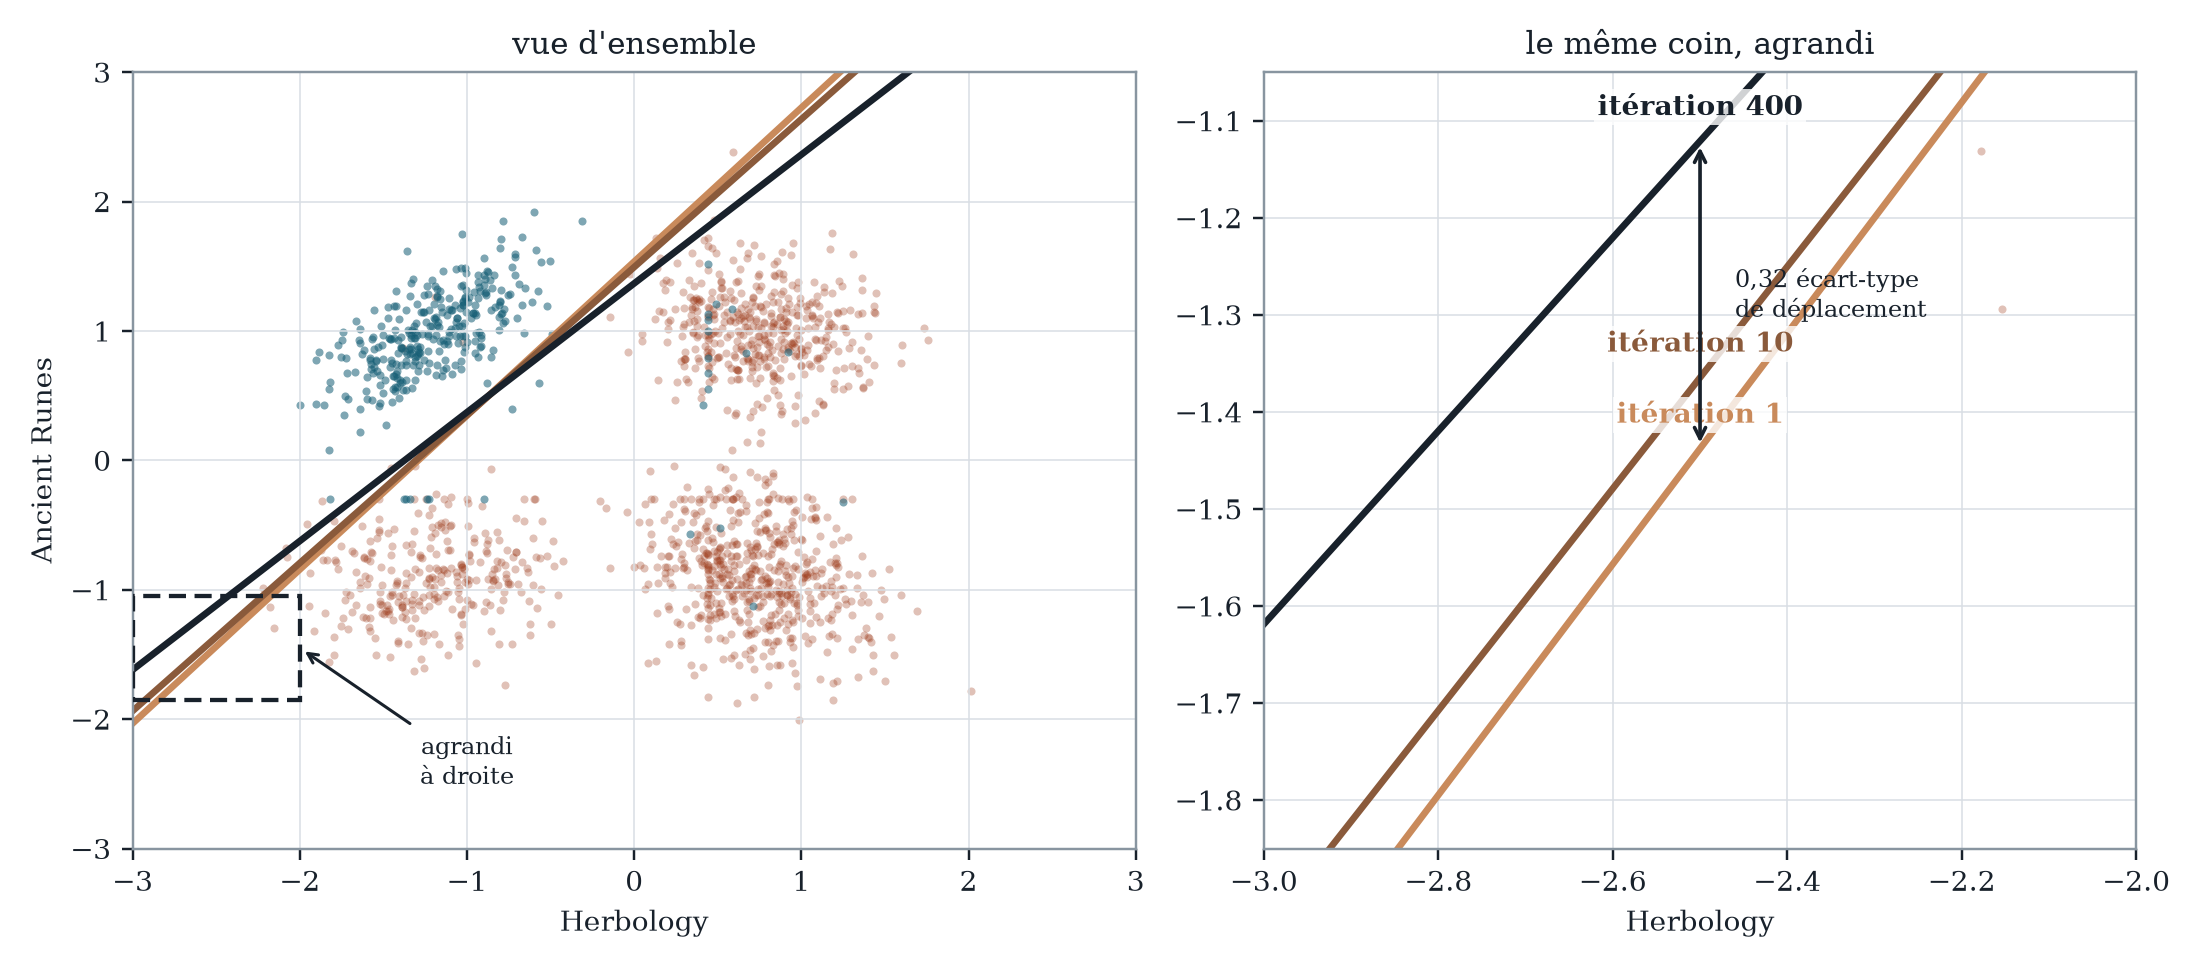
\includegraphics[width=\textwidth]{figures/zoom_droite.png}
\caption{La frontière aux itérations $1$, $10$ et $400$. À l'échelle du nuage,
les trois droites se confondent ; le rectangle agrandi les sépare. Elles pivotent
autour d'un point situé vers le centre du nuage, d'où un écart nul en ce point et
maximal sur les bords. Le déplacement total vaut un tiers d'écart-type.}
\label{fig:zoom}
\end{figure}
\FloatBarrier

Trois cent quatre-vingt-dix-neuf itérations pour un tiers d'écart-type : la
descente consacre donc l'essentiel de son travail à autre chose qu'au
déplacement de cette droite. Pour voir ce travail, il faut regarder la quantité
que la descente modifie réellement, la probabilité, qui est définie en tout point
du plan et pas seulement sur la frontière.

\section{Surface de probabilité}

À chaque point du plan des notes, le modèle associe une probabilité d'appartenir
à \Gryf. Porter cette probabilité en altitude au-dessus du point qui la produit
définit une surface, que les trois figures suivantes donnent aux itérations $1$,
$10$ et $400$.

Le premier tour montre une surface presque plane, traversant le nuage à
mi-hauteur : le modèle répond $0{,}5$ ou presque en tout point, sans distinguer
personne. Au dixième, deux plateaux se dégagent, l'un au-dessus du groupe des
\Gryf, l'autre au-dessus des trois autres, séparés par une pente encore large. Au
quatre centième, les plateaux sont établis et la transition tient sur moins d'un
demi-écart-type.

Une chose reste pourtant fixe d'une figure à l'autre : la ligne noire tracée à
mi-hauteur, où la surface vaut exactement $0{,}5$. Sa projection au sol est la frontière du paragraphe précédent, et c'est de là que
vient sa quasi-immobilité pendant que la surface, elle, change du tout au tout.

\begin{figure}[p]
\centering
\makebox[\textwidth][c]{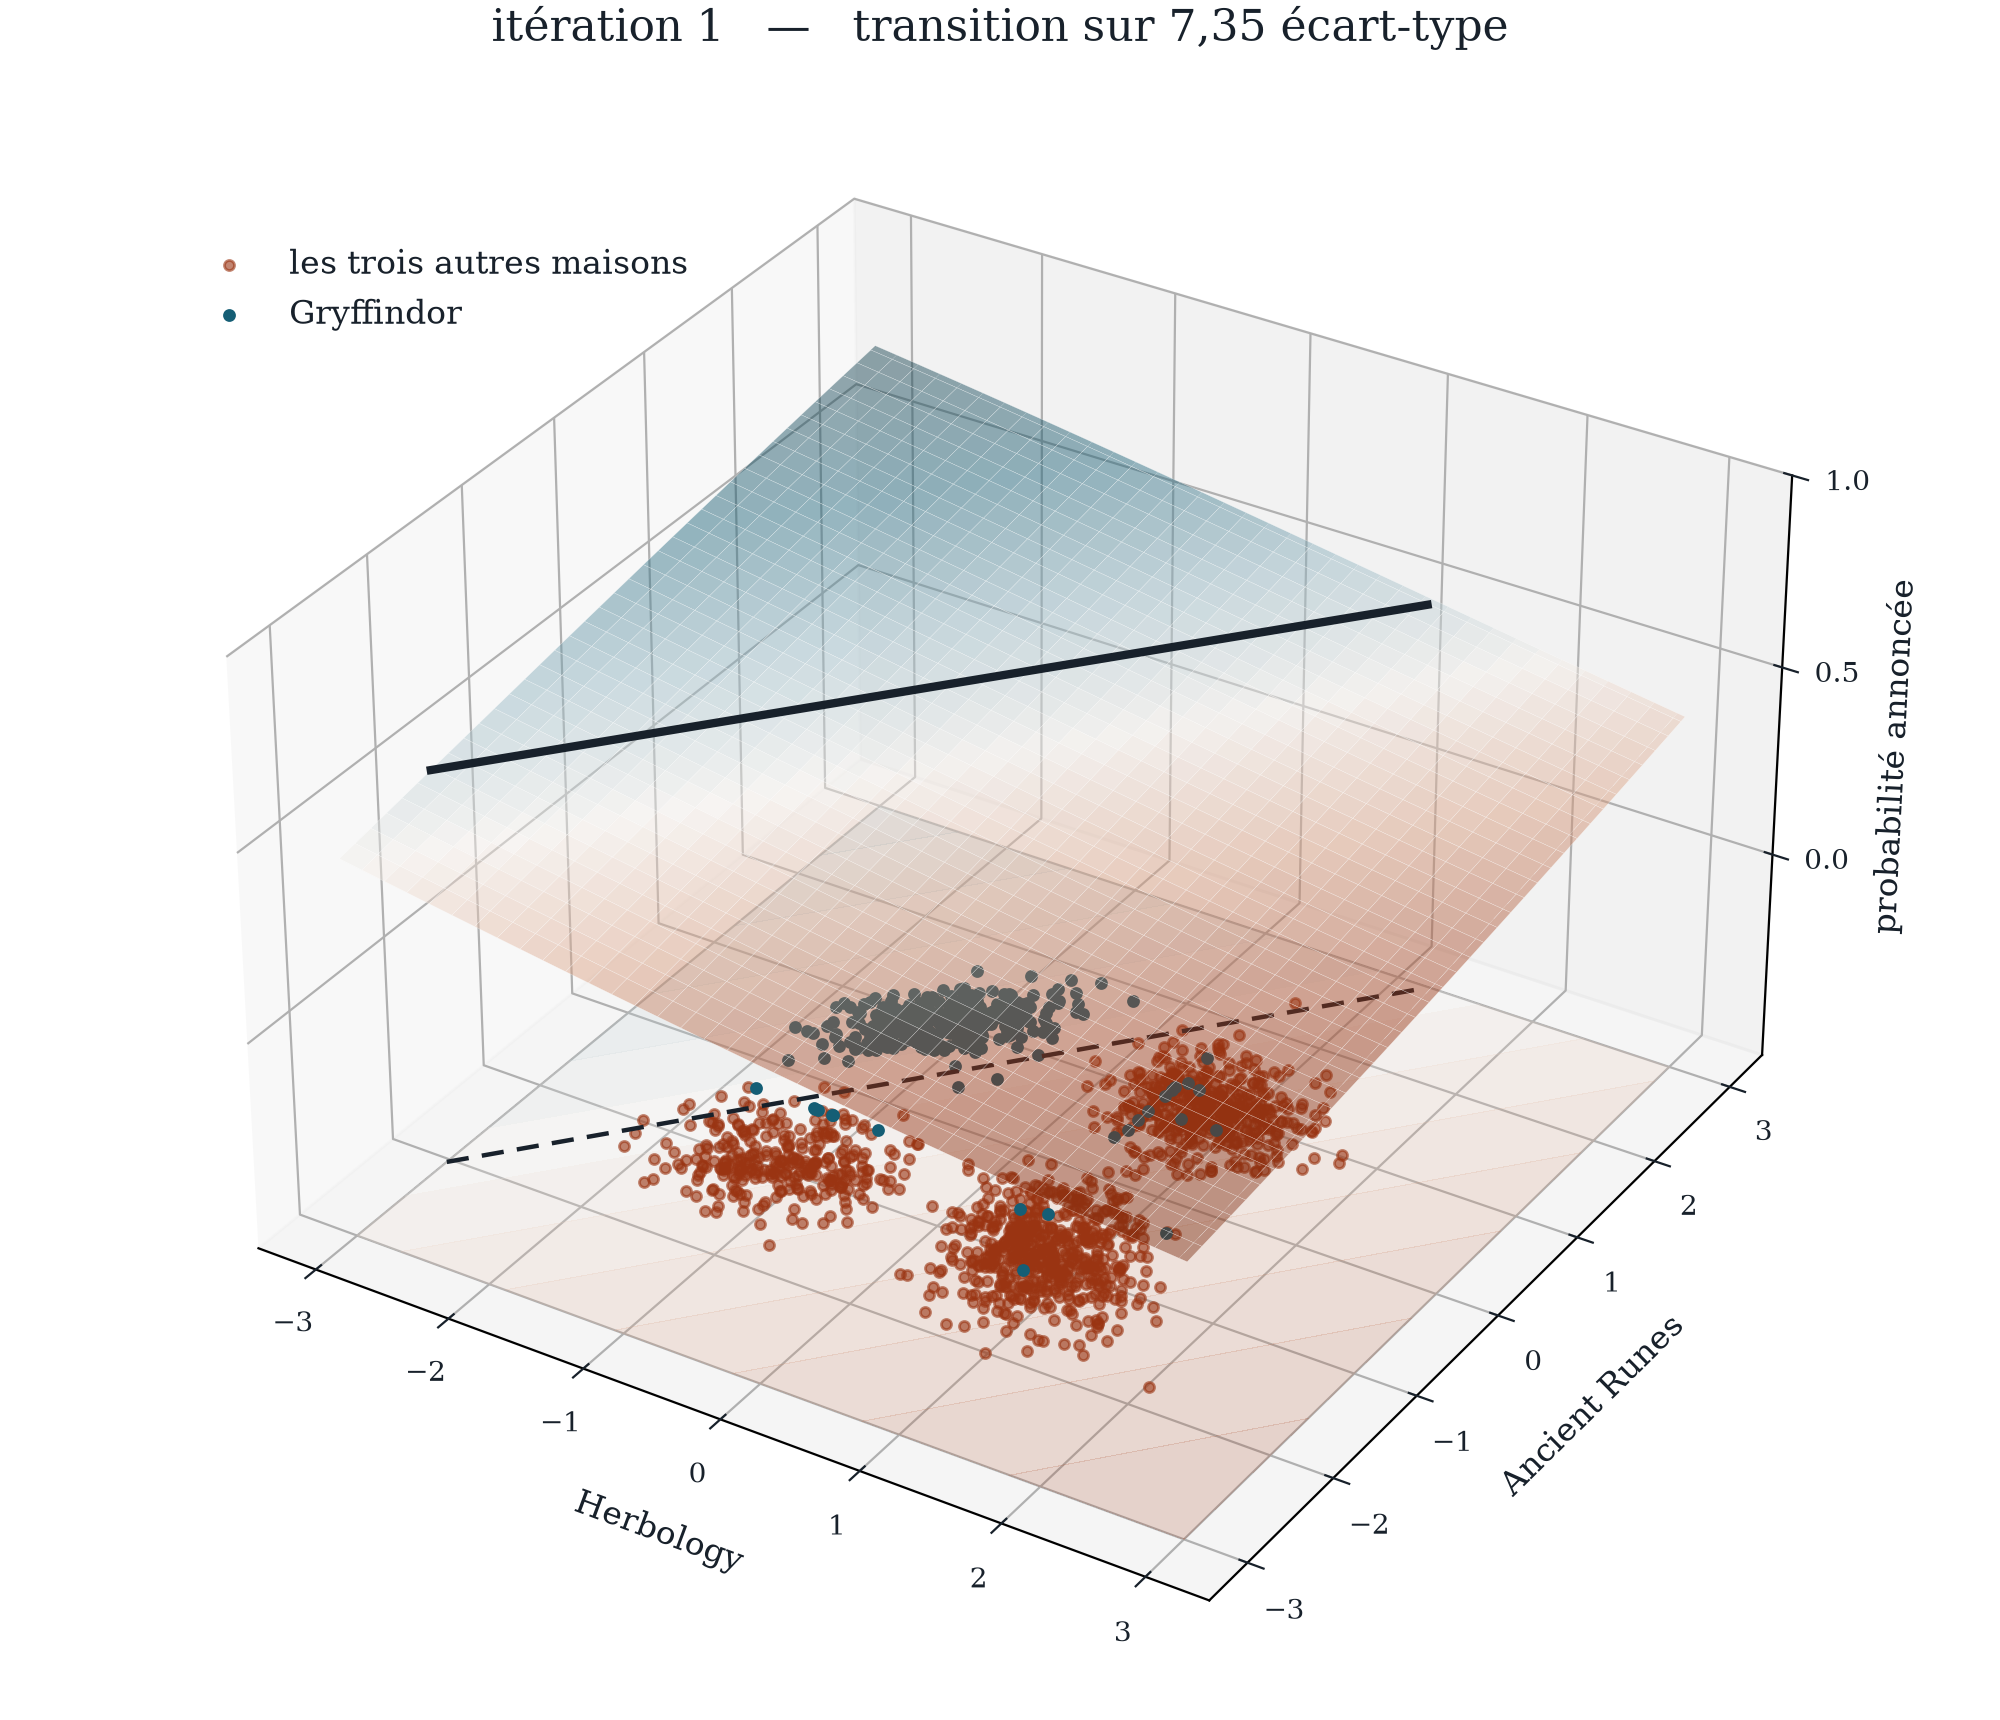
\includegraphics[width=1.28\textwidth]{figures/nappe_it1.png}}
\caption{Premier tour. La surface est presque plane et traverse le nuage à
mi-hauteur : le modèle répond $0{,}5$ ou presque en tout point, et la couleur
reste pâle au-dessus des quatre groupes d'élèves. La ligne noire marque les
$50\,\%$, le pointillé sa projection dans le plan des notes.}
\label{fig:champ}
\end{figure}

\begin{figure}[p]
\centering
\makebox[\textwidth][c]{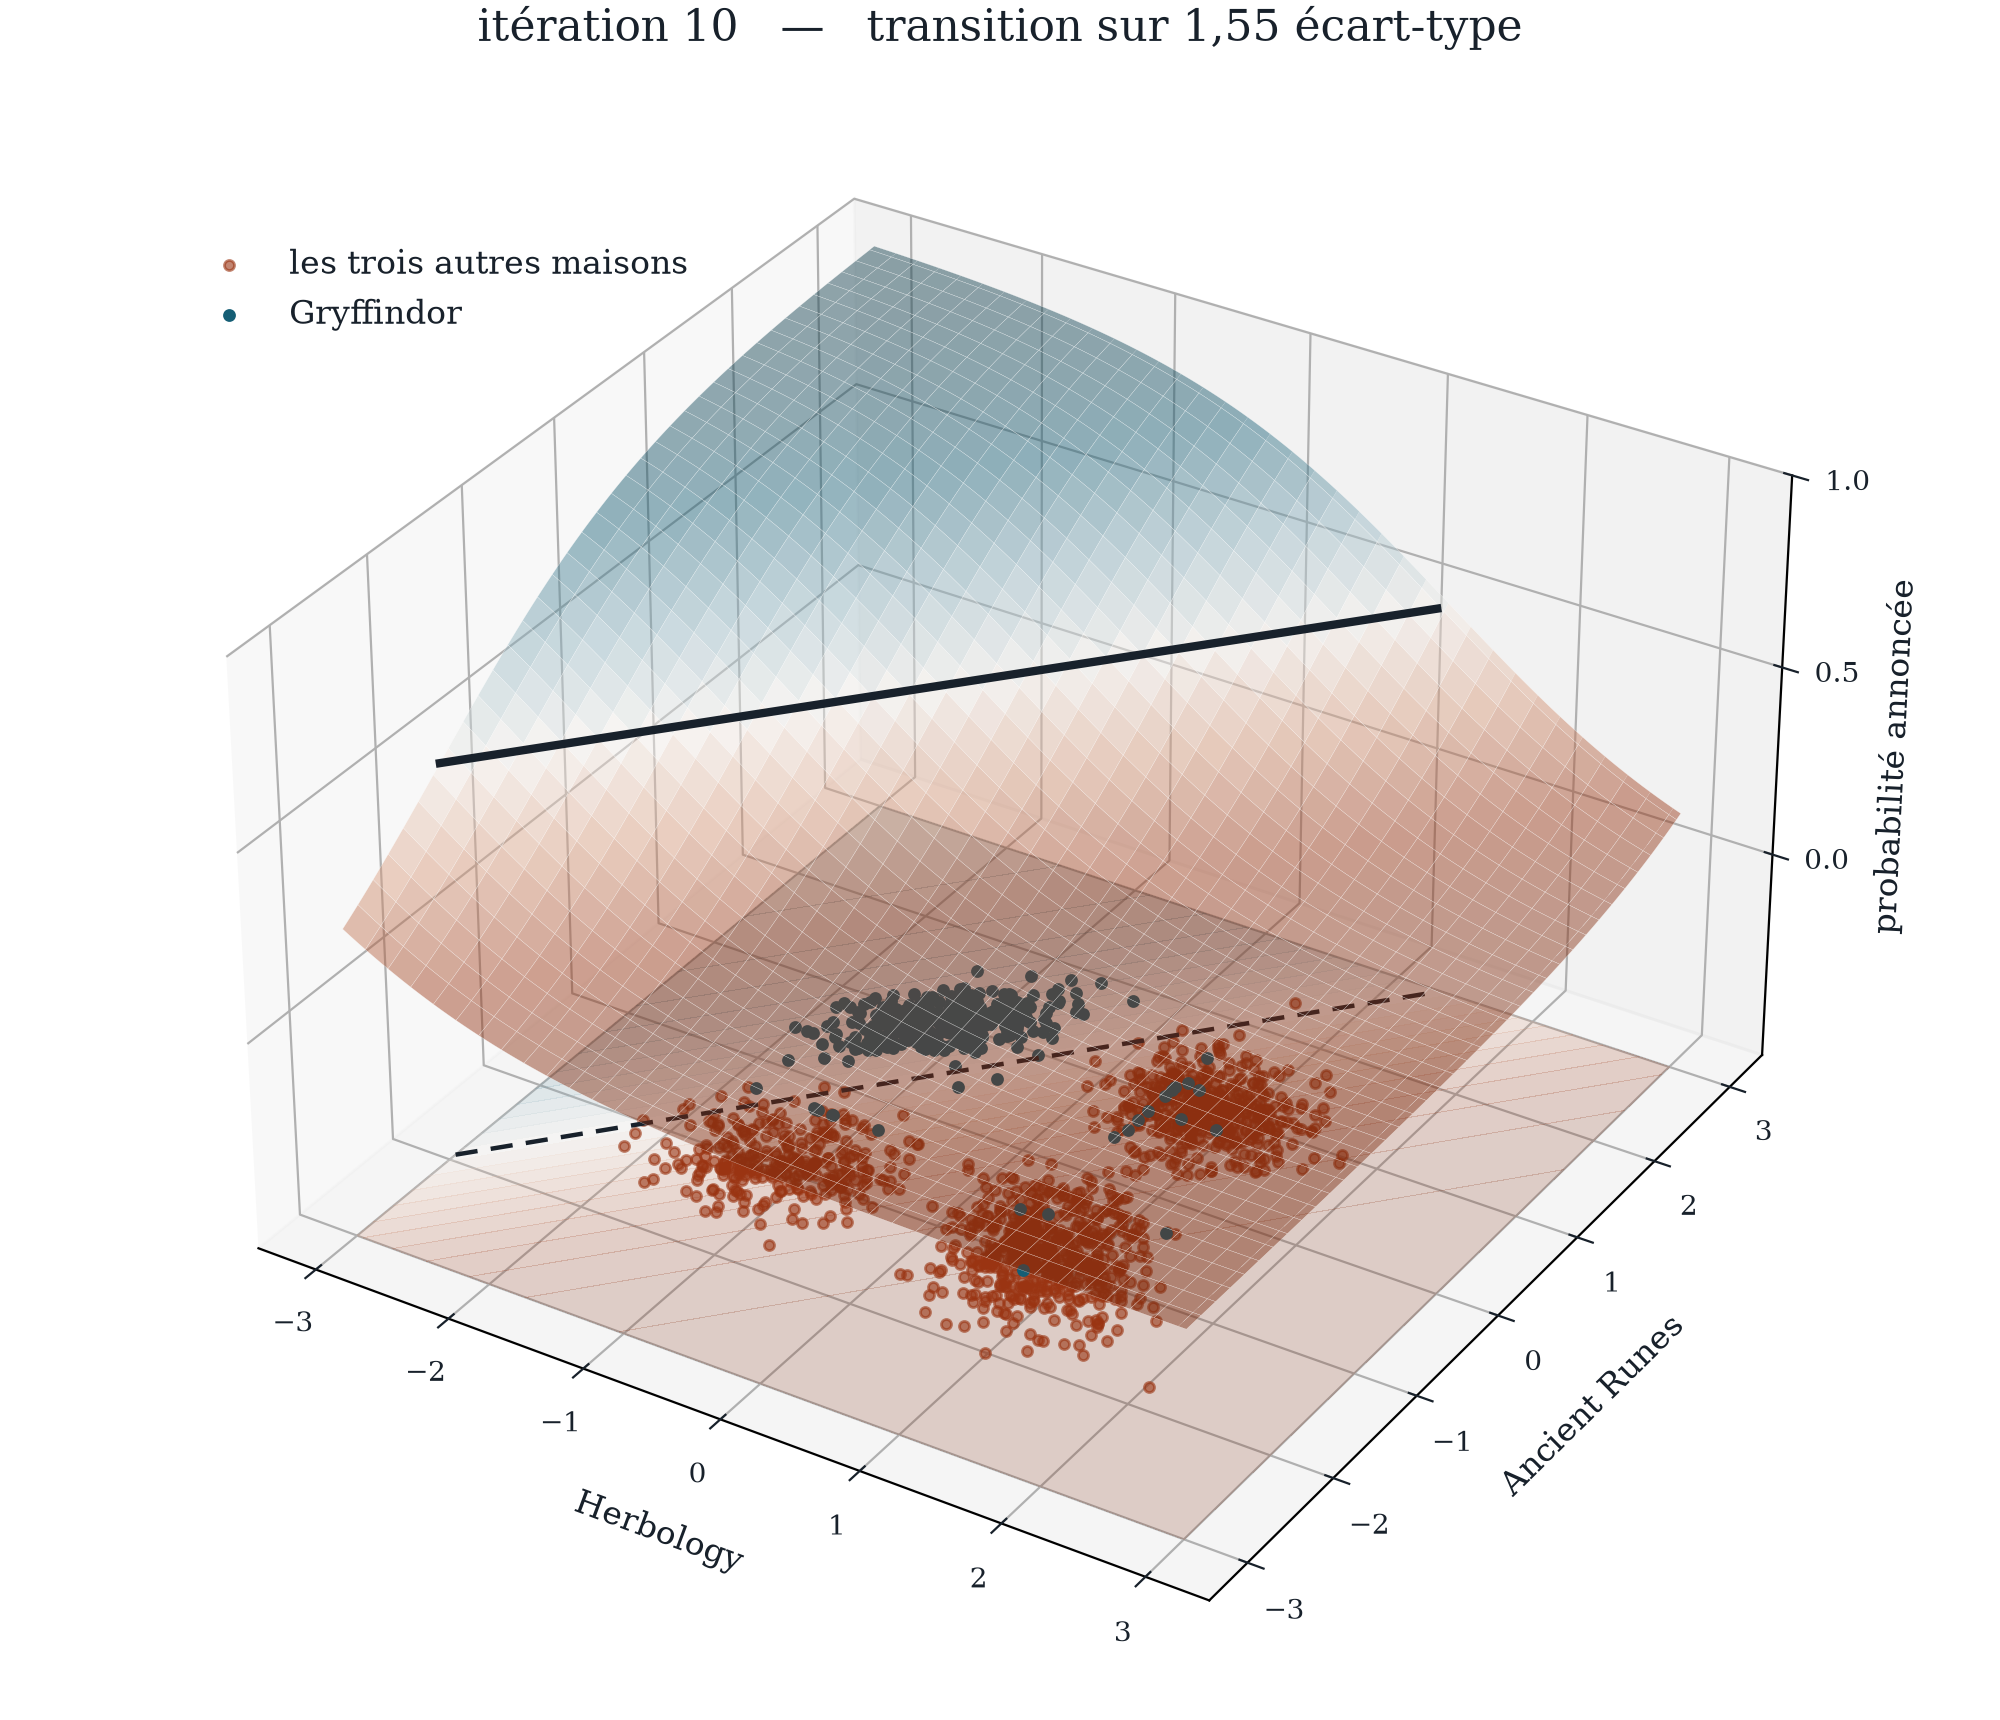
\includegraphics[width=1.28\textwidth]{figures/nappe_it10.png}}
\caption{Dixième tour. Les deux plateaux apparaissent, la transition s'est
resserrée d'un facteur cinq, et les couleurs se différencient au-dessus des
groupes.}
\label{fig:champ10}
\end{figure}

\begin{figure}[p]
\centering
\makebox[\textwidth][c]{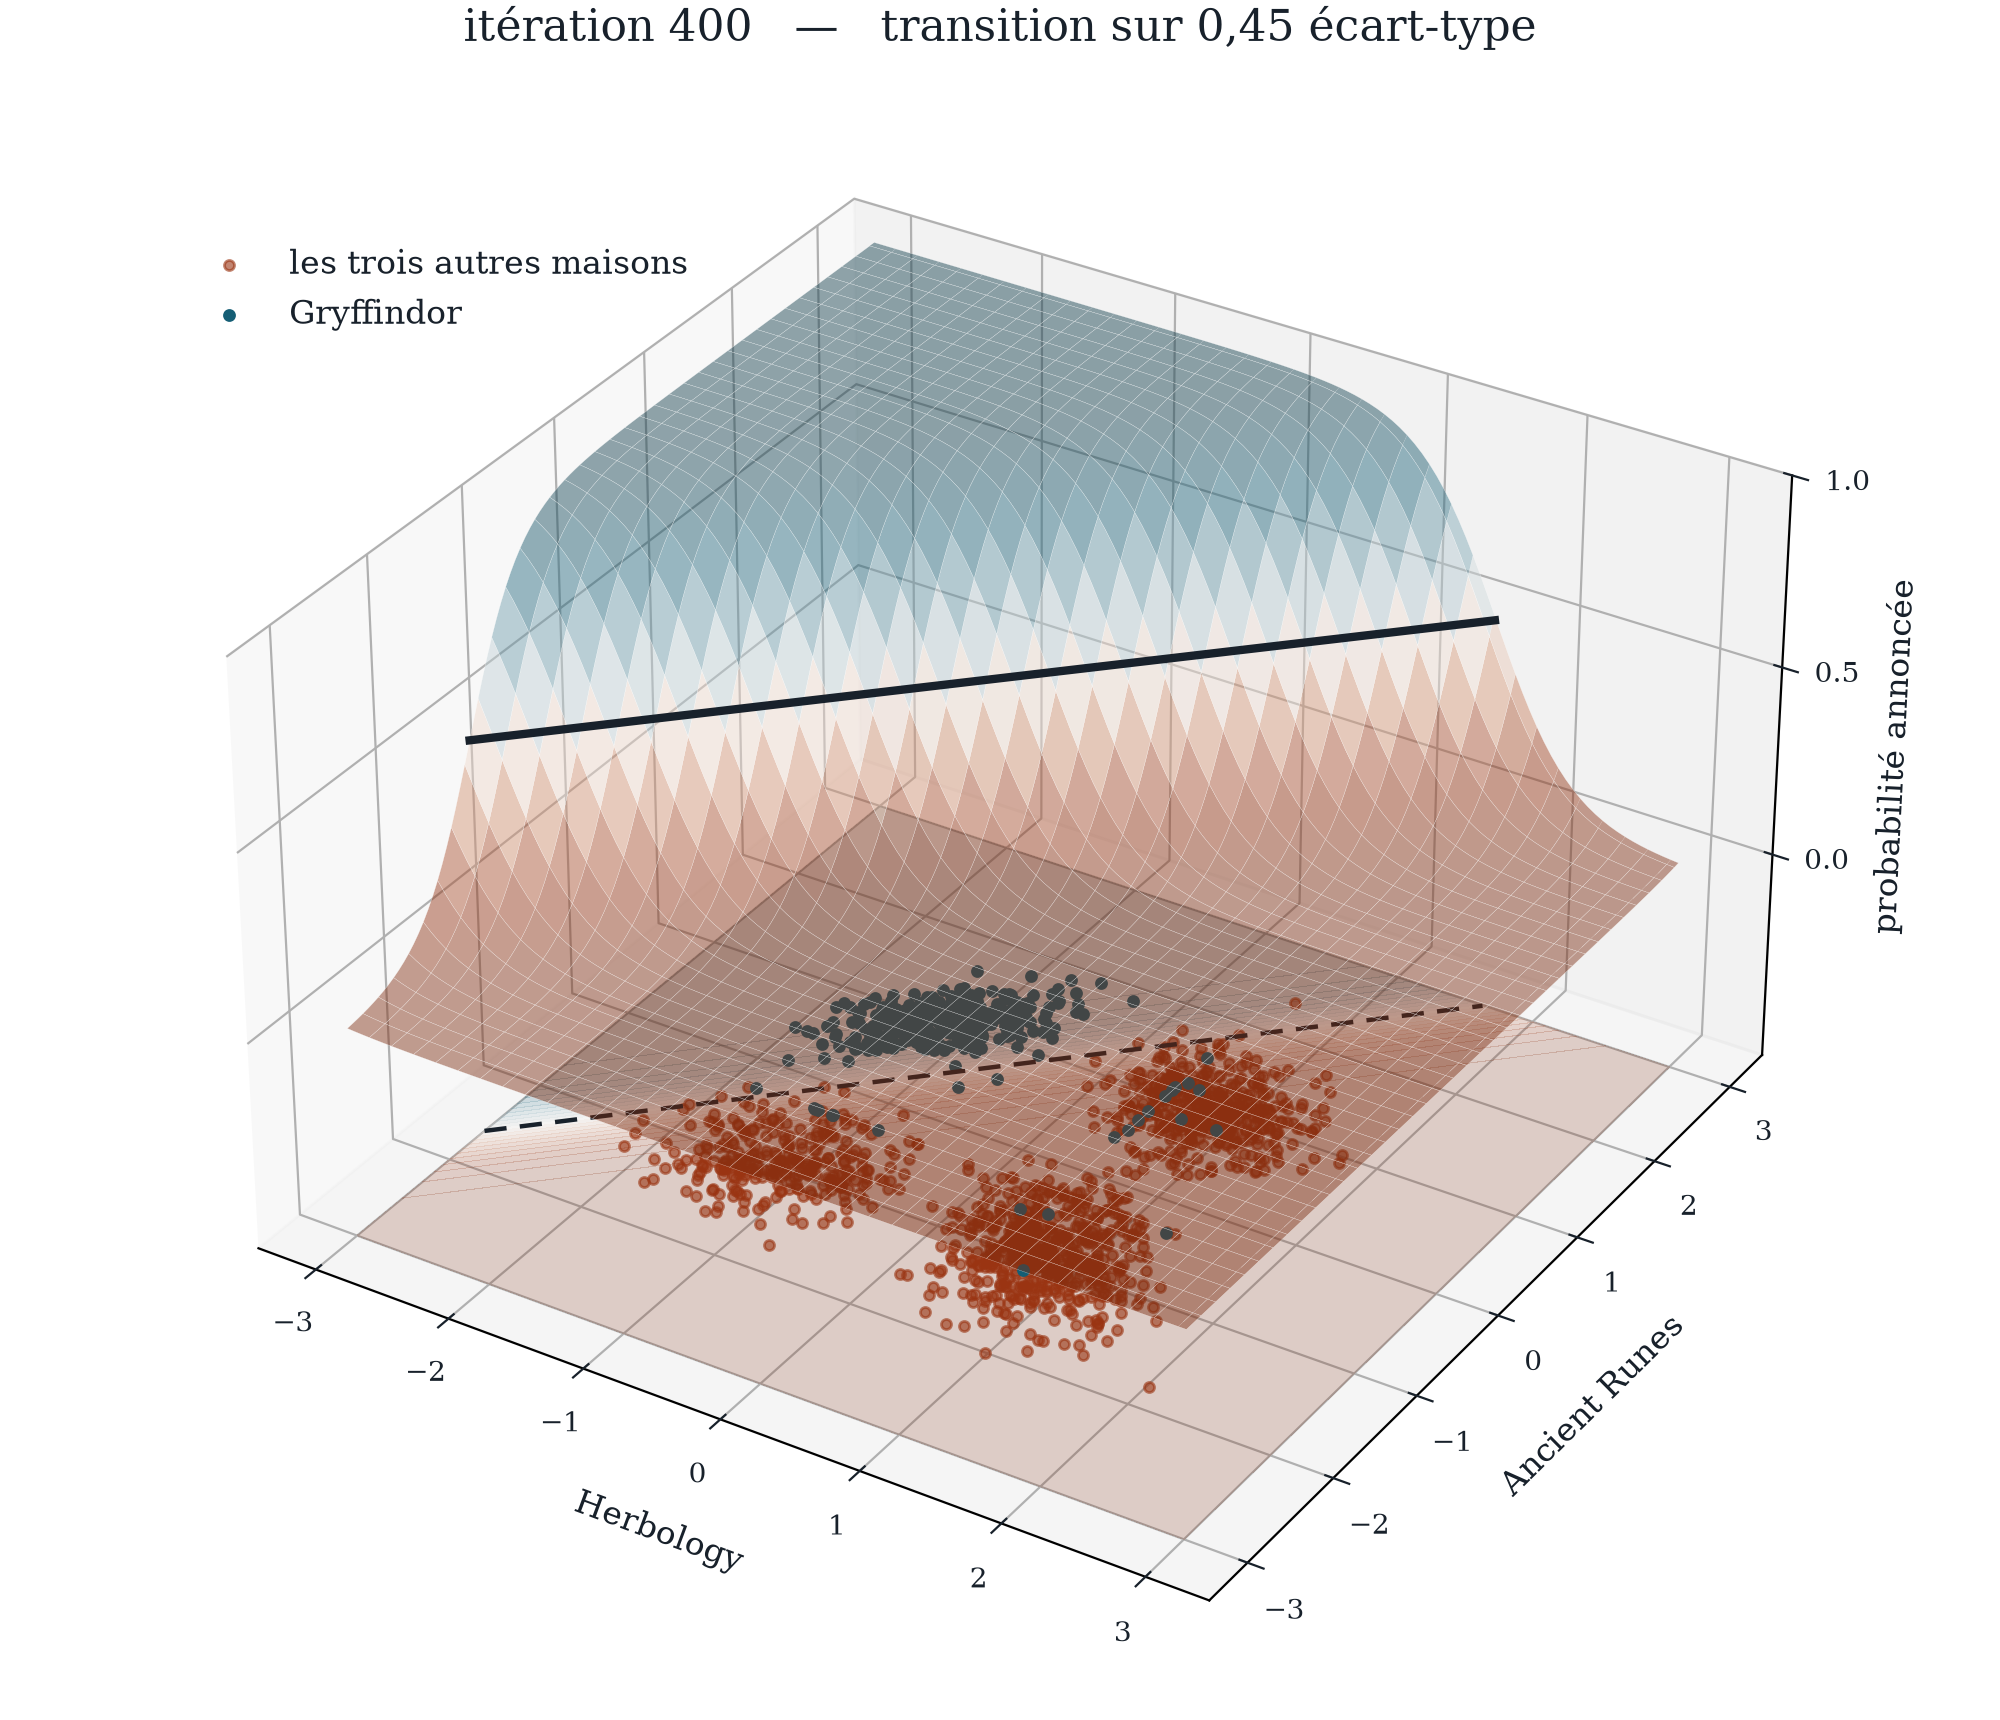
\includegraphics[width=1.28\textwidth]{figures/nappe_it400.png}}
\caption{Quatre centième tour. Le plateau bleu couvre le groupe des \Gryf,
le plateau brun les trois autres, et la transition tient sur moins d'un
demi-écart-type. La couleur indique la maison prédite ; les zones pâles sont
celles où la probabilité reste proche de $0{,}5$.}
\label{fig:champ400}
\end{figure}
\FloatBarrier

\section{Niveau \texorpdfstring{$0{,}5$}{0,5} de la sigmoïde}

Cette surface est la sigmoïde (ch.~\ref{ch:probabilite}) composée avec le
score. La frontière tracée jusqu'ici est le lieu où elle vaut exactement
$0{,}5$.

Notons $d$ la distance d'un élève à la frontière, comptée perpendiculairement et
affectée du signe du côté où il se situe. Alors
\[
  z=\|w\|\,d
  \qquad\text{donc}\qquad
  p=\sigma\bigl(\|w\|\,d\bigr) .
\]
Le rapport des coefficients fixe la position de la frontière (ch.~\ref{ch:nuage})
et leur norme $\|w\|$ fixe la rapidité avec laquelle la probabilité passe de $0$ à
$1$ de part et d'autre : les deux quantités agissent séparément. Relevée le long de cette
perpendiculaire,
la probabilité décrit toujours une sigmoïde, d'autant plus comprimée que
$\|w\|$ est grand.

\begin{figure}[htbp]
\centering
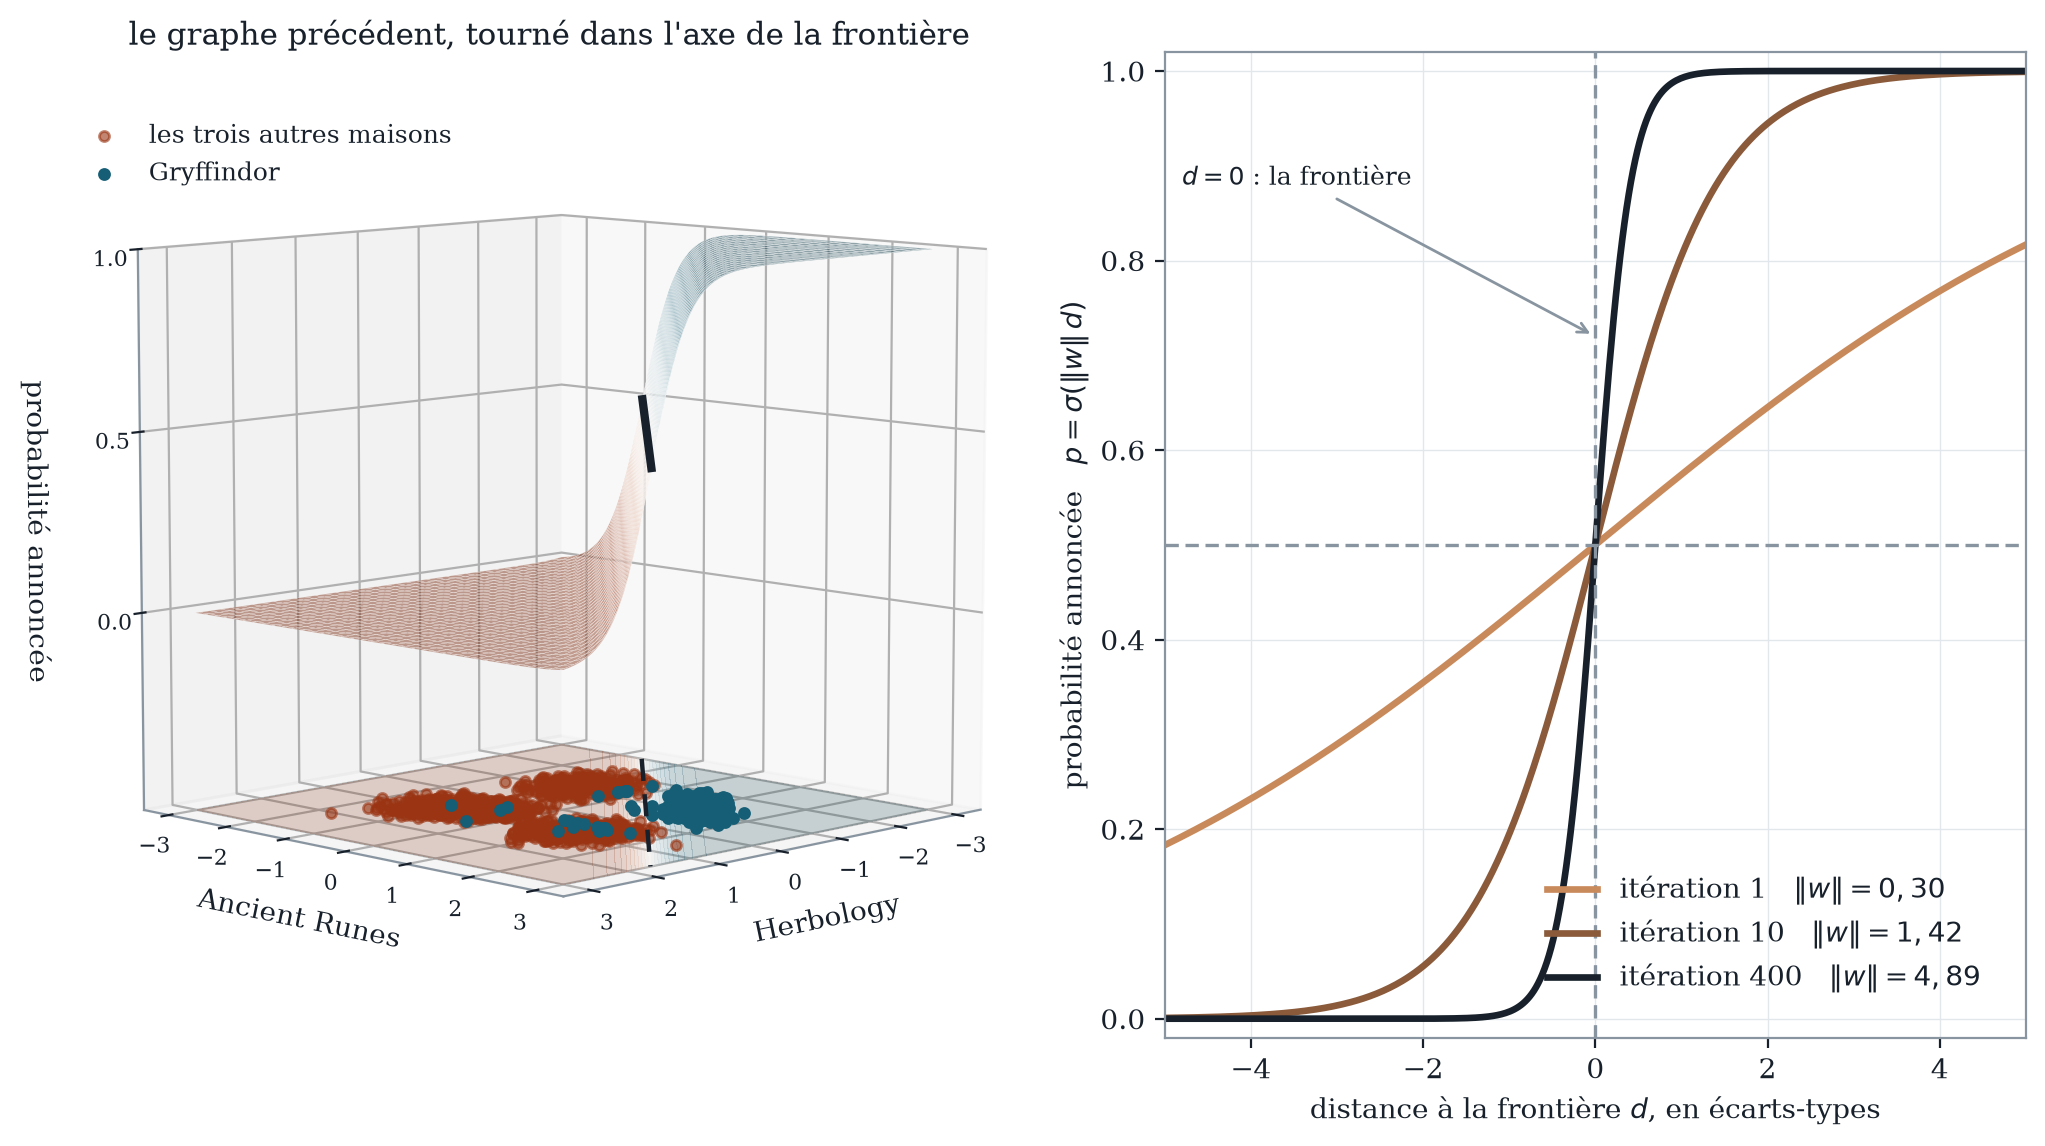
\includegraphics[width=\textwidth]{figures/coupe_sigmoide.png}
\caption{À gauche, le modèle vu de dessus et la direction perpendiculaire à la
frontière. À droite, la probabilité relevée le long de cette direction, aux
trois itérations. Les trois courbes passent par $0{,}5$ à la même abscisse : la
frontière est inchangée. Seule la largeur de la transition varie.}
\label{fig:coupe}
\end{figure}
\FloatBarrier

La largeur de cette transition se mesure par la distance qu'il faut parcourir
pour que la probabilité passe de $25\,\%$ à $75\,\%$, soit $2\log 3/\|w\|$ : elle
est inversement proportionnelle à la norme, et se resserre à mesure que celle-ci grandit.

\begin{releve}
$\|w\|$ passe de $0{,}30$ à $4{,}89$ entre le premier tour et le quatre centième,
et la largeur de transition de $7{,}35$ écarts-types à $0{,}45$ : divisée par
seize, comme la norme est multipliée par seize.
\end{releve}

La frontière, elle, garde sa place : le tracé de la figure~\ref{fig:zoom} le
montrait, les deux courbes de la figure~\ref{fig:suite} le mesurent tour par
tour.

\begin{figure}[htbp]
\centering
\begin{tikzpicture}
\begin{axis}[width=.82\textwidth,height=6cm,
  axis lines=left,axis line style={ink!40},
  grid=major,grid style={gridgray!30},
  tick label style={font=\small},label style={font=\small},
  xlabel={itération},ylabel={norme $\|w\|$},
  xmin=0,xmax=400,ymin=0,ymax=5.4,axis y line*=left]
  \addplot[accent,very thick,no markers] table[x=iter,y=norme] {data/suite.dat};
  \node[font=\small,text=accent,anchor=west] at (axis cs:255,4.2) {norme};
\end{axis}
\begin{axis}[width=.82\textwidth,height=6cm,
  axis lines=right,axis line style={warning!50},
  tick label style={font=\small,text=warning},
  label style={font=\small,text=warning},
  ylabel={pente de la frontière},
  xmin=0,xmax=400,ymin=0.90,ymax=1.30,
  axis x line=none,axis y line*=right]
  \addplot[warning,thick,densely dashed,no markers]
    table[x=iter,y=pente] {data/suite.dat};
  \node[font=\small,text=warning,anchor=south west] at (axis cs:150,1.01) {pente};
\end{axis}
\end{tikzpicture}
\caption{La pente de la frontière atteint sa valeur finale en une cinquantaine de
tours et n'évolue ensuite que dans la troisième décimale, de $1{,}047$ à
$0{,}996$. tandis que la norme des coefficients croît pendant les trois cent cinquante tours
suivants, de $2{,}84$ à $4{,}89$. Les trois cent cinquante derniers tours resserrent la sigmoïde autour d'une frontière déjà en place.}
\label{fig:suite}
\end{figure}
\FloatBarrier

\begin{resultat}[Régimes successifs]
Quelques itérations suffisent à orienter la frontière. Le reste de la descente
augmente la norme des coefficients, ce qui écarte les probabilités de $0{,}5$ en
conservant chaque décision. Pourtant le coût continue de décroître, puisqu'il baisse dès que la probabilité
accordée à la réponse observée augmente : un
critère d'arrêt fondé sur le coût s'arrête donc bien après que le classement
s'est stabilisé. Cette croissance de la norme trouve elle-même une limite, que
l'annexe~\ref{ann:norme} établit.
\end{resultat}

\section{Surface du coût}

Chaque couple de coefficients produit un coût, calculable sur les mille six cents
élèves. Porter ce coût en altitude au-dessus du couple qui le produit définit une
surface au-dessus du plan $(w_1,w_2)$, dont chaque point représente un modèle
possible. Le coût dépendant de trois coefficients, sa représentation demanderait
quatre dimensions ; fixer le biais à sa valeur finale ramène à deux.

La descente se lit sur cette surface : partant d'un point, elle suit la ligne de
plus grande pente et progresse par pas de longueur proportionnelle à $\alpha$.

Deux propriétés de la surface commandent ce qui précède. Établie par la convexité (ch.~\ref{ch:convexite}), l'unicité du minimum entraîne
que tout point de départ conduit au même modèle. Sa pente décroît par ailleurs à
l'approche de ce minimum, ce qui raccourcit les pas successifs et se
mesure à la figure~\ref{fig:norme}.

\begin{figure}[p]
\centering
\vspace*{\fill}
\makebox[\textwidth][c]{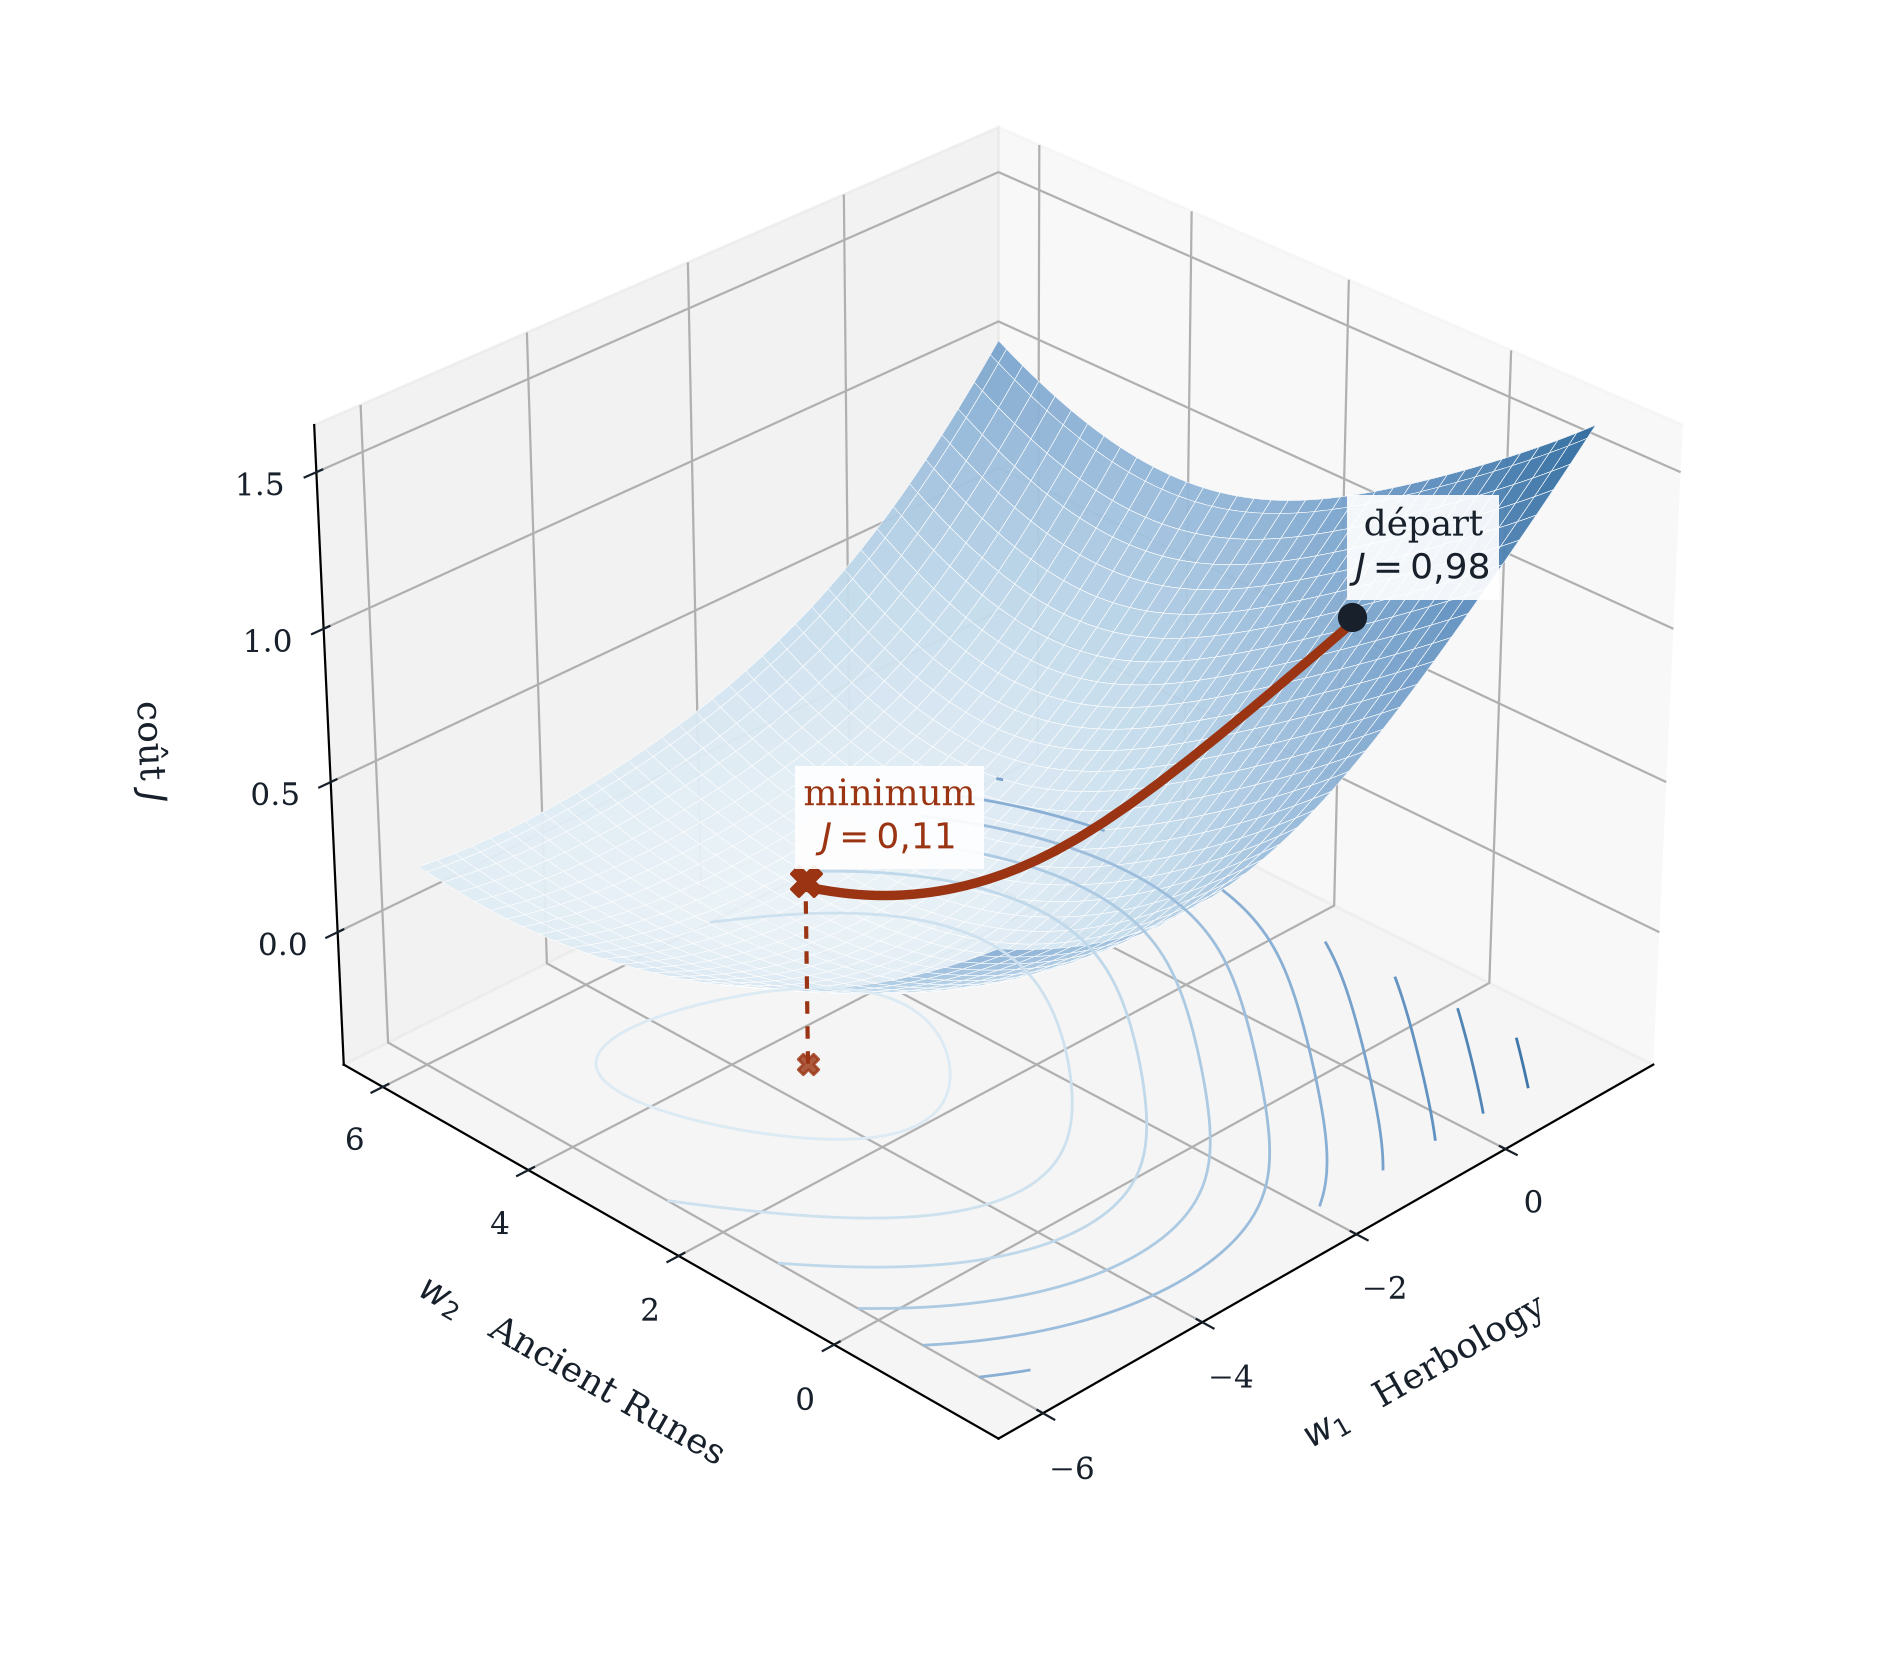
\includegraphics[width=1.12\textwidth]{figures/surface3d.png}}
\caption{La surface du coût au-dessus du plan $(w_1,w_2)$, le biais étant figé à
sa valeur finale. Chaque point du plan horizontal est un couple de coefficients,
et l'altitude au-dessus de lui est le coût que ce couple produit sur les $1\,600$
élèves. La trajectoire rouge part des coefficients nuls et rejoint le
fond. Les courbes tracées au sol sont les lignes de niveau, reprises seules à la
figure~\ref{fig:contours}, où la trajectoire se lit sans perspective.}
\label{fig:surface}
\vspace*{\fill}
\end{figure}

\begin{figure}[htbp]
\centering
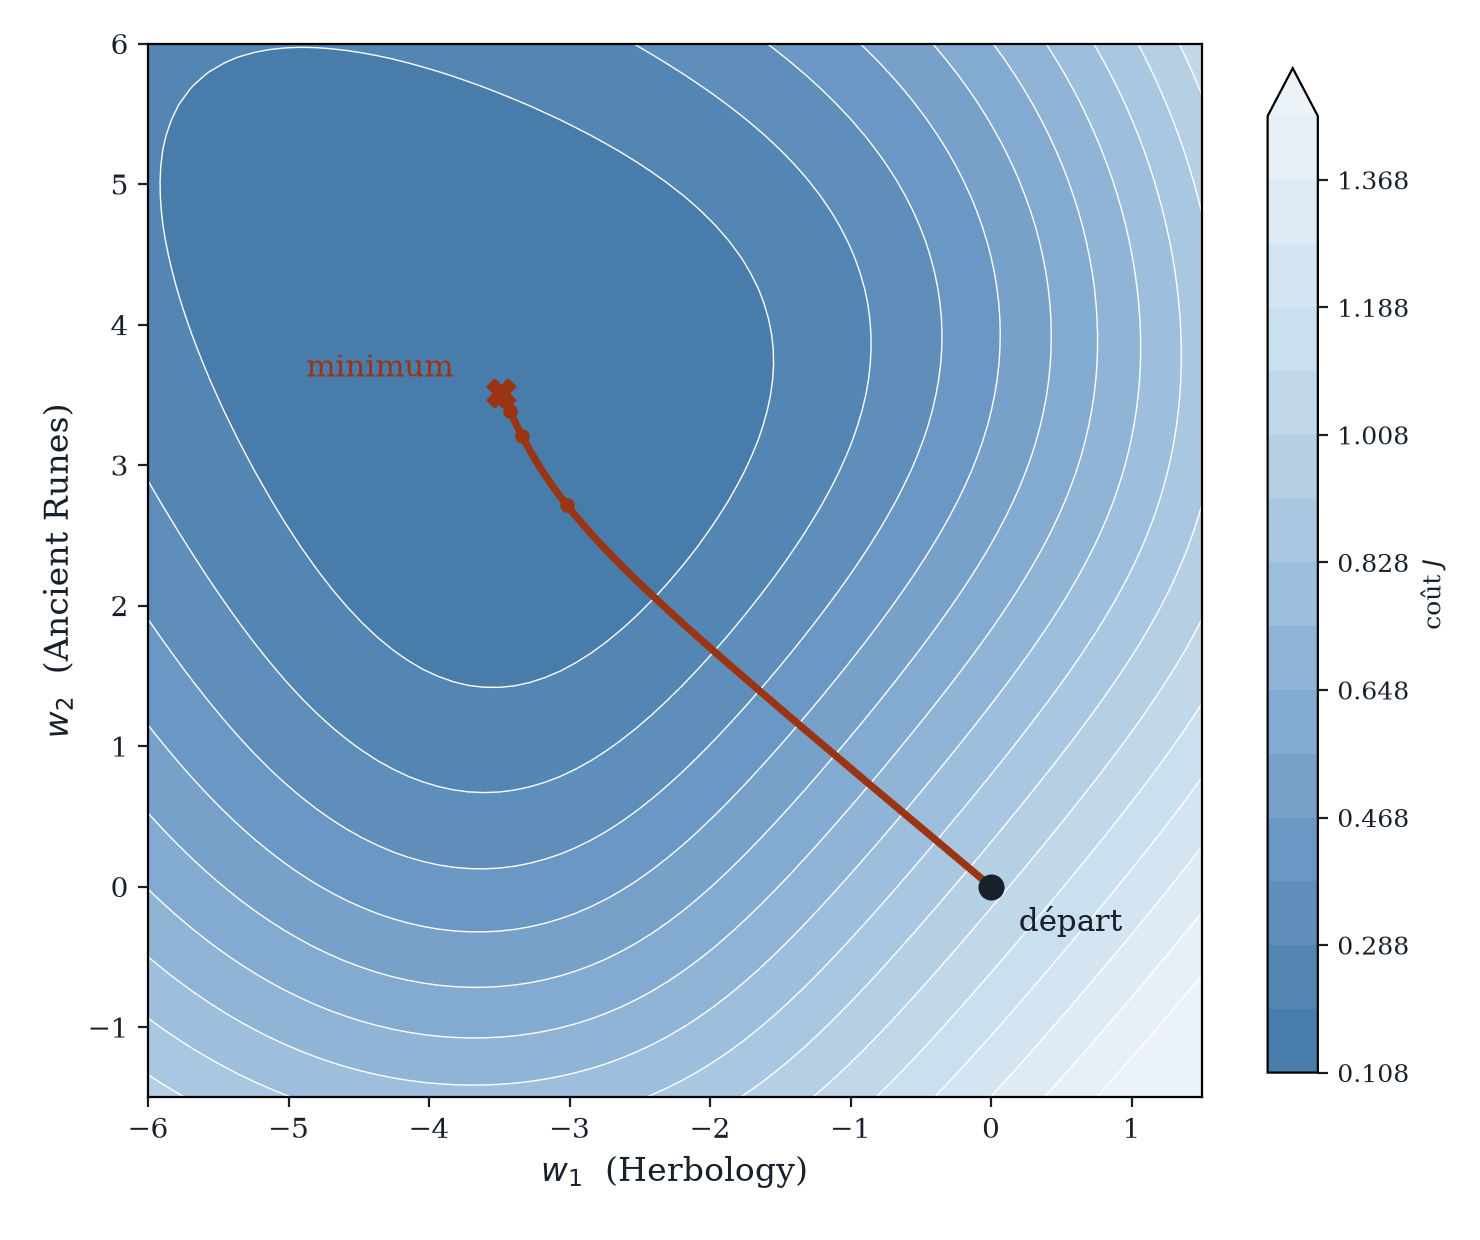
\includegraphics[width=.78\textwidth]{figures/contours.png}
\caption{La même surface vue de dessus. Chaque courbe relie les points de coût
égal, et la trajectoire les coupe perpendiculairement : c'est la propriété du
gradient, qui pointe dans la direction de plus forte pente. Les points marquent
une itération sur vingt-cinq, ce qui rend visible le ralentissement : les
premiers pas traversent plusieurs niveaux, les derniers se resserrent au fond.}
\label{fig:contours}
\end{figure}
\FloatBarrier

\begin{releve}
Le coût passe de $0{,}98$ aux coefficients nuls à $0{,}11$ au minimum, le biais
étant figé à sa valeur finale.
\end{releve}

\section{Longueur du pas}

À chaque tour, le gradient fournit une direction : celle dans laquelle le coût
décroît le plus vite depuis le point où l'on se trouve. Il reste muet sur la
distance à parcourir dans cette direction, et c'est $\alpha$ qui la fixe, en
multipliant le déplacement. Direction et longueur sont deux décisions séparées :
la première se calcule, la seconde se règle.

Un pas court avance peu à chaque tour. La correction disponible n'est consommée
que par fractions, et il en faut d'autant plus pour parcourir la même distance.
Comme un tour demande un passage complet sur les $1\,600$ élèves, le prix se paie
en temps de calcul, pour aboutir à la même frontière.

Un pas long expose au dépassement. Or la pente que donne le gradient ne décrit
fidèlement le terrain qu'au voisinage du point où elle est calculée. Sortir de ce
voisinage fait passer les coefficients de l'autre côté du minimum, sur la pente
opposée, si bien que le coût augmente au lieu de baisser
(figure~\ref{fig:alpha}). Les tours suivants ramènent vers le bas, mais la
trajectoire a fait un détour.

\begin{figure}[htbp]
\centering
\begin{tikzpicture}
\begin{axis}[width=.82\textwidth,height=6.8cm,
  axis lines=left,axis line style={ink!40},
  grid=major,grid style={gridgray!30},
  tick label style={font=\small},label style={font=\small},
  xlabel={itération},ylabel={coût $J$},
  xmin=0,xmax=40,ymin=0.09,ymax=0.72,
  legend style={at={(0.98,0.97)},anchor=north east,draw=none,font=\small,
    fill=white,fill opacity=0.85,text opacity=1}]
  \addplot[warning,very thick,no markers] table[x=iter,y=a005] {data/alpha.dat};
  \addlegendentry{$\alpha=0{,}05$}
  \addplot[huffle,thick,densely dashed,no markers]
    table[x=iter,y=a03] {data/alpha.dat};
  \addlegendentry{$\alpha=0{,}3$}
  \addplot[accent,very thick,no markers] table[x=iter,y=a10] {data/alpha.dat};
  \addlegendentry{$\alpha=1$}
  \addplot[slyth,thick,densely dotted,no markers]
    table[x=iter,y=a1000] {data/alpha.dat};
  \addlegendentry{$\alpha=100$}
\end{axis}
\end{tikzpicture}
\caption{Quarante itérations sur les $1\,600$ élèves, à partir des mêmes
coefficients nuls. Le pas le plus court laisse la courbe très au-dessus des
autres : il lui faudrait des centaines de tours pour les rejoindre. Le pas le
plus long fait remonter le coût dès le premier déplacement, avant de redescendre.}
\label{fig:alpha-reel}
\end{figure}
\FloatBarrier

\begin{chiffres}[Coût moyen selon le pas]
\begin{center}
\begin{tabular}{crrrl}
\toprule
$\alpha$ & départ & après un tour & après quarante & \\
\midrule
$0{,}05$ & $0{,}693$ & $0{,}684$ & $0{,}467$ & pas trop court \\
$0{,}3$  & $0{,}693$ & $0{,}642$ & $0{,}238$ & \\
$1$      & $0{,}693$ & $0{,}539$ & $0{,}153$ & réglage retenu \\
$100$    & $0{,}693$ & $0{,}408$ & $0{,}112$ & dépassement au premier pas \\
\bottomrule
\end{tabular}
\end{center}
Les quatre partent du même coût, $\log 2=0{,}693$, puisque les coefficients
nuls donnent $0{,}5$ à tout le monde. À $\alpha=0{,}05$, atteindre $0{,}15$
demanderait plusieurs centaines de tours pour la même frontière. À $\alpha=100$,
le premier pas emmène les coefficients au-delà du minimum, et la trajectoire
revient ensuite par l'autre versant : quarante tours plus tard, ce réglage a
rattrapé son détour et devancé $\alpha=1$. Ce rattrapage tient à une propriété
de ce coût précisément, établie ci-dessous.
\end{chiffres}

$\alpha$ se règle par essais, en lisant la courbe de coût : un bon réglage la
fait décroître à chaque tour, vite d'abord puis de moins en moins. On retient ici
$\alpha=1$.

\begin{vigilance}[Effet d'un pas excessif]
Le déplacement produit par un pas reste borné quel que soit $\alpha$ : la dérivée
du coût par rapport au score vaut $p-y$, de valeur absolue inférieure à $1$, et
la courbure est majorée par $p(1-p)\leq\frac14$. Un $\alpha$ excessif allonge la trajectoire au lieu de faire exploser les valeurs. Sur ces données,
$\alpha=1\,000$ porte le coût à $6{,}61$ au premier tour, puis le fait
redescendre tour après tour.
\end{vigilance}

\begin{figure}[htbp]
\centering
\begin{minipage}[t]{.48\textwidth}
\centering
\begin{tikzpicture}
\begin{axis}[width=.95\linewidth,height=5.4cm,axis lines=left,
  title={$\alpha$ adapté},xlabel={itération},ylabel={$\theta$},
  xmin=0,xmax=6,ymin=-2.6,ymax=6.6,grid=major,grid style={gridgray!45}]
  \addplot[accent,very thick,mark=*] coordinates
    {(0,-2) (1,0) (2,1) (3,1.5) (4,1.75) (5,1.875) (6,1.9375)};
  \addplot[ink,dashed,thick,domain=0:6]{2};
\end{axis}
\end{tikzpicture}
\end{minipage}\hfill
\begin{minipage}[t]{.48\textwidth}
\centering
\begin{tikzpicture}
\begin{axis}[width=.95\linewidth,height=5.4cm,axis lines=left,
  title={$\alpha$ trop grand},xlabel={itération},ylabel={$\theta$},
  xmin=0,xmax=6,ymin=-2.6,ymax=6.6,grid=major,grid style={gridgray!45}]
  \addplot[warning,very thick,mark=*] coordinates
    {(0,-2) (1,6) (2,-2) (3,6) (4,-2) (5,6) (6,-2)};
  \addplot[ink,dashed,thick,domain=0:6]{2};
\end{axis}
\end{tikzpicture}
\end{minipage}
\caption{Le cas général, sur une fonction quadratique d'une seule variable dont
le minimum est en $2$. À gauche le coefficient s'en approche, à droite il oscille
entre deux valeurs sans converger. Ce second comportement suppose une courbure
croissant avec la distance ; celle du coût logistique reste majorée par
$\frac14$.}
\label{fig:alpha}
\end{figure}
\FloatBarrier

\begin{resultat}[Critères d'arrêt]
Deux critères, employés ensemble. Le premier compare deux coûts successifs : si
la baisse relative passe sous $\varepsilon$, la descente a convergé. Le
second est un plafond d'itérations, qui borne le temps de calcul lorsque le
premier tarde à se déclencher. Sur les $1\,600$ élèves, la baisse relative passe
sous $10^{-6}$ bien après que la frontière a cessé de se déplacer
de façon perceptible : convergence numérique et stabilité des décisions sont deux
choses distinctes.
\end{resultat}

% !TeX root = ../regression_logistique.tex
\chapter{Interprétation du modèle ajusté}
\label{ch:modele}

\orient{%
lire le signe et la valeur d'un coefficient standardisé sans surinterpréter ;
énoncer le contenu complet d'un modèle enregistré ; distinguer paramètres ajustés
et décisions préalables}{%
cote et logit (\annexeref{ann:prerequis}) ; chapitre~\ref{ch:descente}}{%
essentiel}

\section{Interprétation des coefficients}

La descente s'arrête sur trois nombres, qui portent tout ce que l'ajustement a
extrait des $1\,600$ observations :
\[
  w_0=-4{,}745,\qquad
  w_1=-3{,}454\ \text{(\Herb)},\qquad
  w_2=+3{,}469\ \text{(\Runes)} .
\]

Le \emph{signe} donne le sens de l'effet. Le coefficient d'\Herb est négatif :
à note d'\Runes fixée, une note d'\Herb plus haute abaisse le score, donc la
probabilité annoncée. Celui d'\Runes est positif : l'effet est inverse. Dans le
nuage, les \Gryf occupent ainsi la région en haut à gauche.

La \emph{valeur absolue} mesure l'effet d'un écart-type de cette variable sur la
log-cote, \emph{les autres variables restant fixées}. Les deux valeurs $3{,}45$
et $3{,}47$ sont presque égales : un écart-type de l'une ou de l'autre déplace le
score de la même quantité. Cette comparaison n'a de sens que parce que les notes
ont été standardisées : sur les notes brutes, le coefficient d'\Runes serait
vingt fois plus petit que celui d'\Herb pour la seule raison que ses valeurs sont
vingt fois plus dispersées.

La portée de cette lecture est celle d'un effet conditionnel. Avec des variables
corrélées, retirer une colonne modifie les coefficients de celles qui restent,
parfois jusqu'au changement de signe ; un coefficient nul signifie « aucun apport
une fois les autres variables connues ». L'ajustement porte par ailleurs sur des
associations observées, et laisse ouverte la question de savoir si agir sur une
note modifierait la classe. Classer des variables par $|w_j|$ suppose donc des
colonnes standardisées et peu corrélées, et reste une lecture descriptive du
modèle.

Le \emph{biais} $w_0$ est le seul des trois à s'appliquer identiquement à toutes
les observations. Il vaut la log-cote prédite pour une observation dont toutes
les notes standardisées sont nulles, c'est-à-dire moyennes dans chaque matière.

Le biais égale le logit de la proportion de \Gryf dans le seul cas d'un modèle
réduit au biais, sans variable --- le cas du premier pas de la descente. Dès que
des variables corrélées à la classe entrent dans
le score, il s'en écarte : ici $\sigma(-4{,}745)=0{,}0087$, contre une proportion
observée de $0{,}2044$.

Ces trois nombres se lisent aussi de façon quantitative, en revenant à la cote.
Le score étant le logarithme de la cote, ajouter une unité à une note
standardisée augmente le score de $w_j$, donc multiplie la cote par $e^{w_j}$ :
\[
  \frac{p'/(1-p')}{p/(1-p)}=e^{\,w_j}
  \qquad\text{lorsque } x_j \text{ augmente de } 1 .
\]
Un écart-type de plus en \Runes multiplie ainsi par $e^{3{,}469}=32$ la cote
d'appartenir à \Gryf, la note d'\Herb restant fixée ; un écart-type de plus en
\Herb la divise par $e^{3{,}454}=32$ également, les deux coefficients étant
presque opposés. Le biais donne la cote prédite pour une observation moyenne dans
les deux matières : $e^{-4{,}745}=0{,}0087$, soit une chance sur cent quinze.

Les deux panneaux ci-dessous font varier $w_0$ puis $w_1$ autour du modèle
obtenu, les autres coefficients restant à leur valeur. Un troisième panneau pour
$w_2$ montrerait un pivotement identique à celui de $w_1$ : c'est le rapport
$w_1/w_2$ qui fixe la direction de la frontière, et le faire varier par l'un ou
par l'autre revient au même.

\begin{figure}[htbp]
\centering
\begin{graphique}{Deux nuages de points identiques, chacun traversé par trois droites. À gauche, seul le biais varie : les trois droites sont parallèles. À droite, seul le coefficient d'Herbology varie : les trois droites pivotent autour d'un même point. Le trait épais est le modèle obtenu.}
\begin{tikzpicture}[baseline=(current bounding box.north),
  alt={Nuage de points traversé par trois droites parallèles. Seul le biais varie ; le trait épais représente le modèle ajusté.}]
\begin{axis}[panel,width=.46\textwidth,height=6cm,
  title={variation de $w_0$\\[-1pt] \scriptsize
    $w_1=-3{,}454$,\ $w_2=+3{,}469$},
  title style={align=center},
  xlabel={\Herb},ylabel={\Runes}]
  \addplot[only marks,mark=x,mark size=1.1pt,line width=.3pt,warning!80,opacity=.45]
    table[x=x,y=y] {data/autres.dat};
  \addplot[only marks,mark=*,mark size=.8pt,accent,opacity=.6]
    table[x=x,y=y] {data/gryffindor.dat};
  \addplot[ink!35,thick,domain=-2.8:2.8]{(2.0+3.4535*x)/3.4688};
  \addplot[ink,very thick,domain=-2.8:2.8]{(4.7454+3.4535*x)/3.4688};
  \addplot[ink!35,thick,domain=-2.8:2.8]{(7.5+3.4535*x)/3.4688};
\end{axis}
\end{tikzpicture}\hfill
\begin{tikzpicture}[baseline=(current bounding box.north),
  alt={Nuage de points traversé par trois droites qui pivotent autour d'un même point. Seul le coefficient d'Herbology varie ; le trait épais représente le modèle ajusté.}]
\begin{axis}[panel,width=.46\textwidth,height=6cm,
  title={variation de $w_1$\\[-1pt] \scriptsize
    $w_0=-4{,}745$,\ $w_2=+3{,}469$},
  title style={align=center},
  xlabel={\Herb},yticklabels={}]
  \addplot[only marks,mark=x,mark size=1.1pt,line width=.3pt,warning!80,opacity=.45]
    table[x=x,y=y] {data/autres.dat};
  \addplot[only marks,mark=*,mark size=.8pt,accent,opacity=.6]
    table[x=x,y=y] {data/gryffindor.dat};
  \addplot[ink!35,thick,domain=-2.8:2.8]{(4.7454+1.2*x)/3.4688};
  \addplot[ink,very thick,domain=-2.8:2.8]{(4.7454+3.4535*x)/3.4688};
  \addplot[ink!35,thick,domain=-2.8:2.8]{(4.7454+7.0*x)/3.4688};
\end{axis}
\end{tikzpicture}
\end{graphique}
\caption{Variation isolée du biais, à gauche : translation. Variation isolée de
$w_1$, à droite : rotation et modification de la pente de la sigmoïde.}
\label{fig:roles}
\end{figure}
\FloatBarrier

\begin{figure}[htbp]
\centering
\begin{graphique}{Trois blocs. En haut à gauche, les trois coefficients ajustés. En haut à droite, les conventions : ordre des matières et réponse associée. En bas, un tableau des statistiques d'entraînement donnant médiane, moyenne et écart-type pour chacune des deux matières.}
\begin{tikzpicture}[
  bx/.style={draw=ink!30,rounded corners=2.5pt,inner sep=6pt,align=center},
  ttl/.style={font=\footnotesize\bfseries,text=ink,anchor=base}]

\node[bx,fill=accentlight,minimum height=15mm] (w) at (0,0)
  {\footnotesize$\begin{array}{r@{\;=\;}r}
     w_0 & -4{,}745\\ w_1 & -3{,}454\\ w_2 & +3{,}469
   \end{array}$};
\node[bx,fill=warninglight,minimum height=15mm,right=8mm of w] (cv)
  {\footnotesize\begin{tabular}{@{}ll@{}}
     ordre des matières : & \Herb, \Runes\\[2pt]
     réponse associée : & \Gryf ou non
   \end{tabular}};
\node[ttl,above=2.5mm of w] {coefficients ajustés};
\node[ttl,above=2.5mm of cv] {conventions};

\coordinate (mid) at ($(w.south)!0.5!(cv.south)$);
\node[bx,fill=rulelight,below=10mm of mid,anchor=north] (st)
  {\footnotesize\begin{tabular}{@{}lrrr@{}}
     \toprule
     matière & médiane & moyenne & écart-type\\
     \midrule
     \Herb  & $3{,}469$   & $1{,}189$   & $5{,}175$\\
     \Runes & $463{,}918$ & $495{,}052$ & $105{,}186$\\
     \bottomrule
   \end{tabular}};
\node[ttl,above=2mm of st] {statistiques d'entraînement};
\end{tikzpicture}
\end{graphique}
\caption{Contenu d'un modèle enregistré, référence unique pour tout le document :
coefficients, six statistiques de préparation, ordre des matières et réponse
associée. Chaque élément est nécessaire à la prédiction.}
\label{fig:contenu-modele}
\end{figure}
\FloatBarrier

\section{Paramètres appris et paramètres fixés}

Les trois coefficients sortent du calcul ; tout le reste a été décidé avant lui,
et d'autres décisions auraient donné un autre modèle sur le même fichier.

\begin{table}[htbp]
\centering
\begin{tabular}{ll>{\raggedright\arraybackslash}p{54mm}}
\toprule
 & valeur ici & ce qui la fixe \\
\midrule
\multicolumn{3}{l}{\textbf{déterminé par la descente}}\\
\addlinespace[1pt]
coefficients $w$ & les trois valeurs ci-dessus
  & les notes et les maisons du fichier \\
\addlinespace[3pt]
\multicolumn{3}{l}{\textbf{posé avant la descente}}\\
\addlinespace[1pt]
matières retenues & \Herb, \Runes & le choix de deux matières qui se dessinent \\
remplissage des vides & la médiane & un arbitrage entre deux méthodes
  (ch.~\ref{ch:standardisation}) \\
échelle des notes & centrage-réduction & rendre les coefficients comparables \\
coefficients de départ & tous nuls & un point de départ quelconque convient \\
longueur du pas $\alpha$ & $1$ & un essai contrôlé sur la courbe de coût \\
critère d'arrêt & $\varepsilon$ et un plafond & le temps de calcul accordé \\
seuil de décision & $0{,}5$ & les deux erreurs comptées au même prix
  (ch.~\ref{ch:probabilite}) \\
\bottomrule
\end{tabular}
\caption{Le calcul produit trois nombres ; les sept décisions le précèdent.}
\label{tab:appris-pose}
\end{table}
\FloatBarrier

Ces décisions restent invisibles dans les trois coefficients enregistrés, et
doivent être consignées à côté d'eux pour qu'un tiers puisse refaire le
résultat.

\section{Classement d'une observation nouvelle}

Le calcul est celui de la figure~\ref{fig:carte}, la classe n'étant plus connue
mais déduite : standardiser les deux notes avec les statistiques d'entraînement,
calculer $z=w_0+w_1x_1+w_2x_2$, annoncer \Gryf si $z\geq0$. Cette comparaison à
zéro équivaut à comparer $p$ à $0{,}5$, la sigmoïde étant croissante ; le calcul
de $p$ est réservé à l'affichage.

Sur les $1\,600$ lignes du fichier, cette règle en classe correctement $1\,564$.
Les trente-six prédictions incorrectes relèvent de deux situations que la
distance à la frontière sépare.

La première est le recouvrement des deux groupes. Dans la bande où les deux
populations occupent la même région du plan, aucune droite ne peut les séparer
sans erreur, et déplacer la frontière ne fait que changer lesquelles.
Ces prédictions se reconnaissent à leur score, faible en valeur absolue, et à la
probabilité qui l'accompagne, voisine de $0{,}5$.

La seconde tient à des observations dont les notes contredisent l'étiquette.
Situées loin dans la région de l'autre groupe, elles reçoivent une prédiction
incorrecte assortie d'une probabilité élevée : ce sont les observations atypiques
dont la perte individuelle dépasse cent fois la
moyenne. La plus éloignée est incorrectement classée à une distance de
$2{,}27$ écarts-types de la frontière.

\begin{chiffres}[Erreurs par distance à la frontière]
\begin{center}
\begin{tabular}{lrl}
\toprule
distance & prédictions & \\
\midrule
moins de $0{,}5$ écart-type & $20$ & recouvrement des deux groupes \\
de $0{,}5$ à $1{,}0$        & $11$ & \\
plus de $1{,}0$             & $5$  & observations atypiques, jusqu'à $2{,}27$ \\
\midrule
\textbf{total}              & $\mathbf{36}$ & sur $1\,600$, soit $97{,}75\,\%$ de correctes \\
\bottomrule
\end{tabular}
\end{center}
La distance est comptée perpendiculairement à la frontière, en écarts-types, soit
$|z|/\|w\|$.
\end{chiffres}

Le taux de $97{,}75\,\%$ est l'\emph{exactitude sur l'échantillon
d'ajustement} : il sert de contrôle de cohérence, une valeur anormalement basse
signalant un défaut d'ajustement. L'exactitude hors échantillon, assortie de son
incertitude, est mesurée au chapitre~\ref{ch:predire}.

\section{Extension à dix notes et quatre maisons}

Passer de deux notes à dix ajoute huit coefficients et laisse les formules
identiques : la frontière devient un hyperplan de $\R^{10}$. Ce qui change ici
est la taille du fichier enregistré.

\begin{table}[htbp]
\centering
\begin{tabular}{lcccc}
\toprule
 & \multicolumn{2}{c}{\textbf{une maison}} & \multicolumn{2}{c}{\textbf{quatre maisons}} \\
\cmidrule(lr){2-3}\cmidrule(lr){4-5}
matières & coefficients & statistiques & coefficients & statistiques \\
\midrule
$2$  & $3$  & $6$  & $12$ & $6$  \\
$10$ & $11$ & $30$ & $44$ & $30$ \\
$n$  & $n+1$ & $3n$ & $4(n+1)$ & $3n$ \\
\bottomrule
\end{tabular}
\caption{Taille du modèle enregistré. Les coefficients se multiplient par le
nombre de maisons, les statistiques non : médiane, moyenne et écart-type sont
calculés une fois par matière et servent aux quatre modèles.}
\label{tab:taille}
\end{table}

Le passage à quatre maisons ajoute une décision : quatre modèles comme celui-ci
--- \Gryf contre le reste, puis \Huff contre le reste, et ainsi de suite ---
donnent quatre scores pour une même observation, et la classe retenue est celle
du plus grand (ch.~\ref{ch:classifieur}).

\begin{exercice}[Lecture d'un coefficient]
Un modèle ajusté sur les notes \emph{brutes} donnerait $w_2\approx+0{,}033$ pour
\Runes. Montrer que ce coefficient décrit la même frontière que $+3{,}469$, et
dire lequel des deux se compare à celui d'\Herb. Par quel facteur un écart-type
de plus en \Runes multiplie-t-il la cote, et pourquoi ce facteur ne dépend-il pas
de l'échelle retenue ?
\end{exercice}

\chapter{Classification à quatre maisons}
\label{ch:classifieur}

\begin{lecture}
Le modèle construit jusqu'ici répond à une seule question : \Gryf ou non.
Or le problème en compte quatre, dont une réponse unique doit sortir. Pour cela,
la construction réutilise les outils déjà en place : le même ajustement est répété
pour chaque maison, et les quatre scores obtenus sont comparés.
\end{lecture}

\section{Un modèle par maison}

Le modèle construit jusqu'ici répond par oui ou par non, parce qu'une frontière
sépare le plan en deux régions et pas davantage. Quatre maisons demandent une
autre construction, et deux voies s'offrent.

La première consiste à concevoir un modèle qui produise directement quatre
probabilités de somme $1$ : c'est la régression \emph{softmax}, dont la
dérivation diffère de celle menée aux chapitres précédents. La seconde ramène le
problème à quatre questions binaires, chacune traitée par le modèle déjà en
place, puis combine les quatre réponses. C'est cette seconde voie qui est
retenue, parce qu'elle réemploie tout ce qui précède sans y changer une ligne.

Elle porte le nom d'\emph{un contre tous}, ou \emph{one-vs-rest}. Pour chaque
maison, on reprend le procédé à l'identique, seule la cible changeant :
\[
  y_i=1 \text{ si l'élève } i \text{ appartient à la maison traitée},\qquad
  y_i=0 \text{ sinon.}
\]
Les notes et leur préparation sont inchangées, le tableau $\X$ est le même pour
les quatre modèles ; seule la colonne des réponses change.

\begin{figure}[htbp]
\centering
\begin{tikzpicture}[
  cell/.style={draw=ink!25,minimum width=22mm,minimum height=5.6mm,
    font=\scriptsize,inner sep=1.5pt},
  bit/.style={draw=ink!25,minimum width=8mm,minimum height=5.6mm,
    font=\scriptsize,inner sep=1.5pt},
  head/.style={font=\scriptsize\bfseries,text=ink,align=center}]

\node[cell,fill=gryff!12] (m1) {\Gryf};
\node[cell,fill=slyth!12,below=0.5mm of m1] (m2) {\Slyth};
\node[cell,fill=raven!12,below=0.5mm of m2] (m3) {\Rav};
\node[cell,fill=huffle!12,below=0.5mm of m3] (m4) {\Huff};
\node[head,above=2.5mm of m1] {maison};

\foreach \k/\dx/\col/\a/\b/\c/\d in {%
  1/3.2/gryff/1/0/0/0, 2/4.5/huffle/0/0/0/1,
  3/5.8/raven/0/0/1/0, 4/7.1/slyth/0/1/0/0}{
  \node[bit,fill=\col!14] (a\k) at ($(m1)+(\dx,0)$) {$\a$};
  \node[bit,fill=\col!14] (b\k) at ($(m2)+(\dx,0)$) {$\b$};
  \node[bit,fill=\col!14] (c\k) at ($(m3)+(\dx,0)$) {$\c$};
  \node[bit,fill=\col!14] (d\k) at ($(m4)+(\dx,0)$) {$\d$};
}
\node[head,text=gryff,above=2.5mm of a1] {$y^{(G)}$};
\node[head,text=huffle,above=2.5mm of a2] {$y^{(H)}$};
\node[head,text=raven,above=2.5mm of a3] {$y^{(R)}$};
\node[head,text=slyth,above=2.5mm of a4] {$y^{(S)}$};
\end{tikzpicture}
\caption{Quatre colonnes de réponses construites depuis la même colonne de
maisons. Chaque ligne porte exactement un $1$ : les quatre modèles sont ajustés
séparément, mais leurs cibles restent liées par cette contrainte, qu'aucun d'eux
ne connaît.}
\label{fig:quatre-cibles}
\end{figure}
\FloatBarrier

Quatre descentes indépendantes donnent quatre jeux de coefficients. Sur les
deux matières employées ici :

\begin{table}[htbp]
\centering
\begin{tabular}{lrrr}
\toprule
maison traitée & $w_0$ & $w_1$ (\Herb) & $w_2$ (\Runes) \\
\midrule
\Gryf & $-4{,}997$ & $-3{,}625$ & $+3{,}655$ \\
\Huff & $-3{,}056$ & $+3{,}889$ & $-4{,}358$ \\
\Rav  & $-3{,}729$ & $+4{,}061$ & $+3{,}869$ \\
\Slyth  & $-4{,}545$ & $-3{,}341$ & $-3{,}549$ \\
\bottomrule
\end{tabular}
\caption{Les quatre modèles binaires. Chaque maison correspond à un couple de
signes distinct, et les quatre combinaisons possibles sont occupées.}
\label{tab:quatre}
\end{table}

Ces douze nombres se lisent sur le nuage par le procédé du
chapitre~\ref{ch:modele} : le signe de $w_1$ dit de quel côté en \Herb se
trouve la maison traitée, celui de $w_2$ fait de même en \Runes. Les quatre
maisons occupant chacune un coin du nuage, les quatre couples de signes possibles
se trouvent employés, un par maison.

Les quatre biais sont négatifs pour une raison commune : chaque maison est
minoritaire face aux trois autres réunies, si bien qu'un élève pris au hasard
reçoit un score négatif dans les quatre modèles.

\section{Règle du score maximal}

Un nouvel élève reçoit quatre scores, un par maison, et il faut en tirer une
réponse. Chaque score mesure à quel point son modèle penche pour sa maison :
retenir le plus élevé est la règle la plus directe.
\[
  \text{maison prédite}=\arg\max_{k}\ z_k,
  \qquad z_k=w_{k0}+w_{k1}x_1+w_{k2}x_2
\]

Cette règle repose sur une hypothèse qu'il vaut mieux énoncer : que les quatre
scores soient comparables entre eux. Rien ne l'assure a priori, les quatre
modèles ayant été ajustés séparément, chacun sur sa propre question. Deux
éléments la rendent acceptable ici. Tous partagent la même famille de fonctions et les mêmes notes standardisées,
donc la même échelle d'entrée ; et la sigmoïde, croissante et identique pour tous, convertit chaque
score en probabilité de la même manière, si bien que comparer les scores ou les
probabilités donne la même réponse. La décision se prend sur les scores, et les
probabilités ne se calculent que pour être affichées.

Un seuil de $0{,}5$ appliqué séparément à chaque modèle produirait un autre
résultat : il pourrait ne désigner aucune maison, si les quatre probabilités
tombaient en dessous, ou plusieurs à la fois. La règle du maximum désigne
toujours exactement une maison, quelle que soit la valeur des scores.

\begin{releve}
L'élève $3$, de notes standardisées $x_1=-1{,}485$ et $x_2=+0{,}275$, donne
\begin{align*}
  z_G &= -4{,}997-3{,}625\times(-1{,}485)+3{,}655\times0{,}275 = +1{,}393,\\
  z_H &= -3{,}056+3{,}889\times(-1{,}485)-4{,}358\times0{,}275 = -10{,}031,\\
  z_R &= -3{,}729+4{,}061\times(-1{,}485)+3{,}869\times0{,}275 = \phantom{0}-8{,}697,\\
  z_S &= -4{,}545-3{,}341\times(-1{,}485)-3{,}549\times0{,}275 = \phantom{0}-0{,}558.
\end{align*}
\end{releve}

Le maximum est $z_G$, et la maison prédite est celle de l'élève. Le deuxième score se tient près de deux unités en dessous.

\begin{table}[htbp]
\centering
\begin{tabular}{crrrrl}
\toprule
élève & $z_G$ & $z_H$ & $z_R$ & $z_S$ & prédiction \\
\midrule
$3$   & $\mathbf{+1{,}393}$ & $-10{,}031$ & $-8{,}697$ & $-0{,}558$
      & \Gryf, sa maison \\
$571$ & $-6{,}829$ & $-1{,}125$ & $\mathbf{-1{,}046}$ & $-6{,}781$
      & \Rav, alors qu'il est \Huff \\
\bottomrule
\end{tabular}
\caption{Deux élèves passés aux quatre modèles ; le score retenu est en gras.
L'élève $571$ départage \Rav et \Huff sur un écart de $0{,}079$, et la règle se
trompe. Ses quatre scores sont négatifs, ce qui signifie que les quatre modèles
binaires répondent « non » : le maximum reste le moins mauvais des quatre.}
\label{tab:deux-eleves}
\end{table}

\begin{figure}[htbp]
\centering
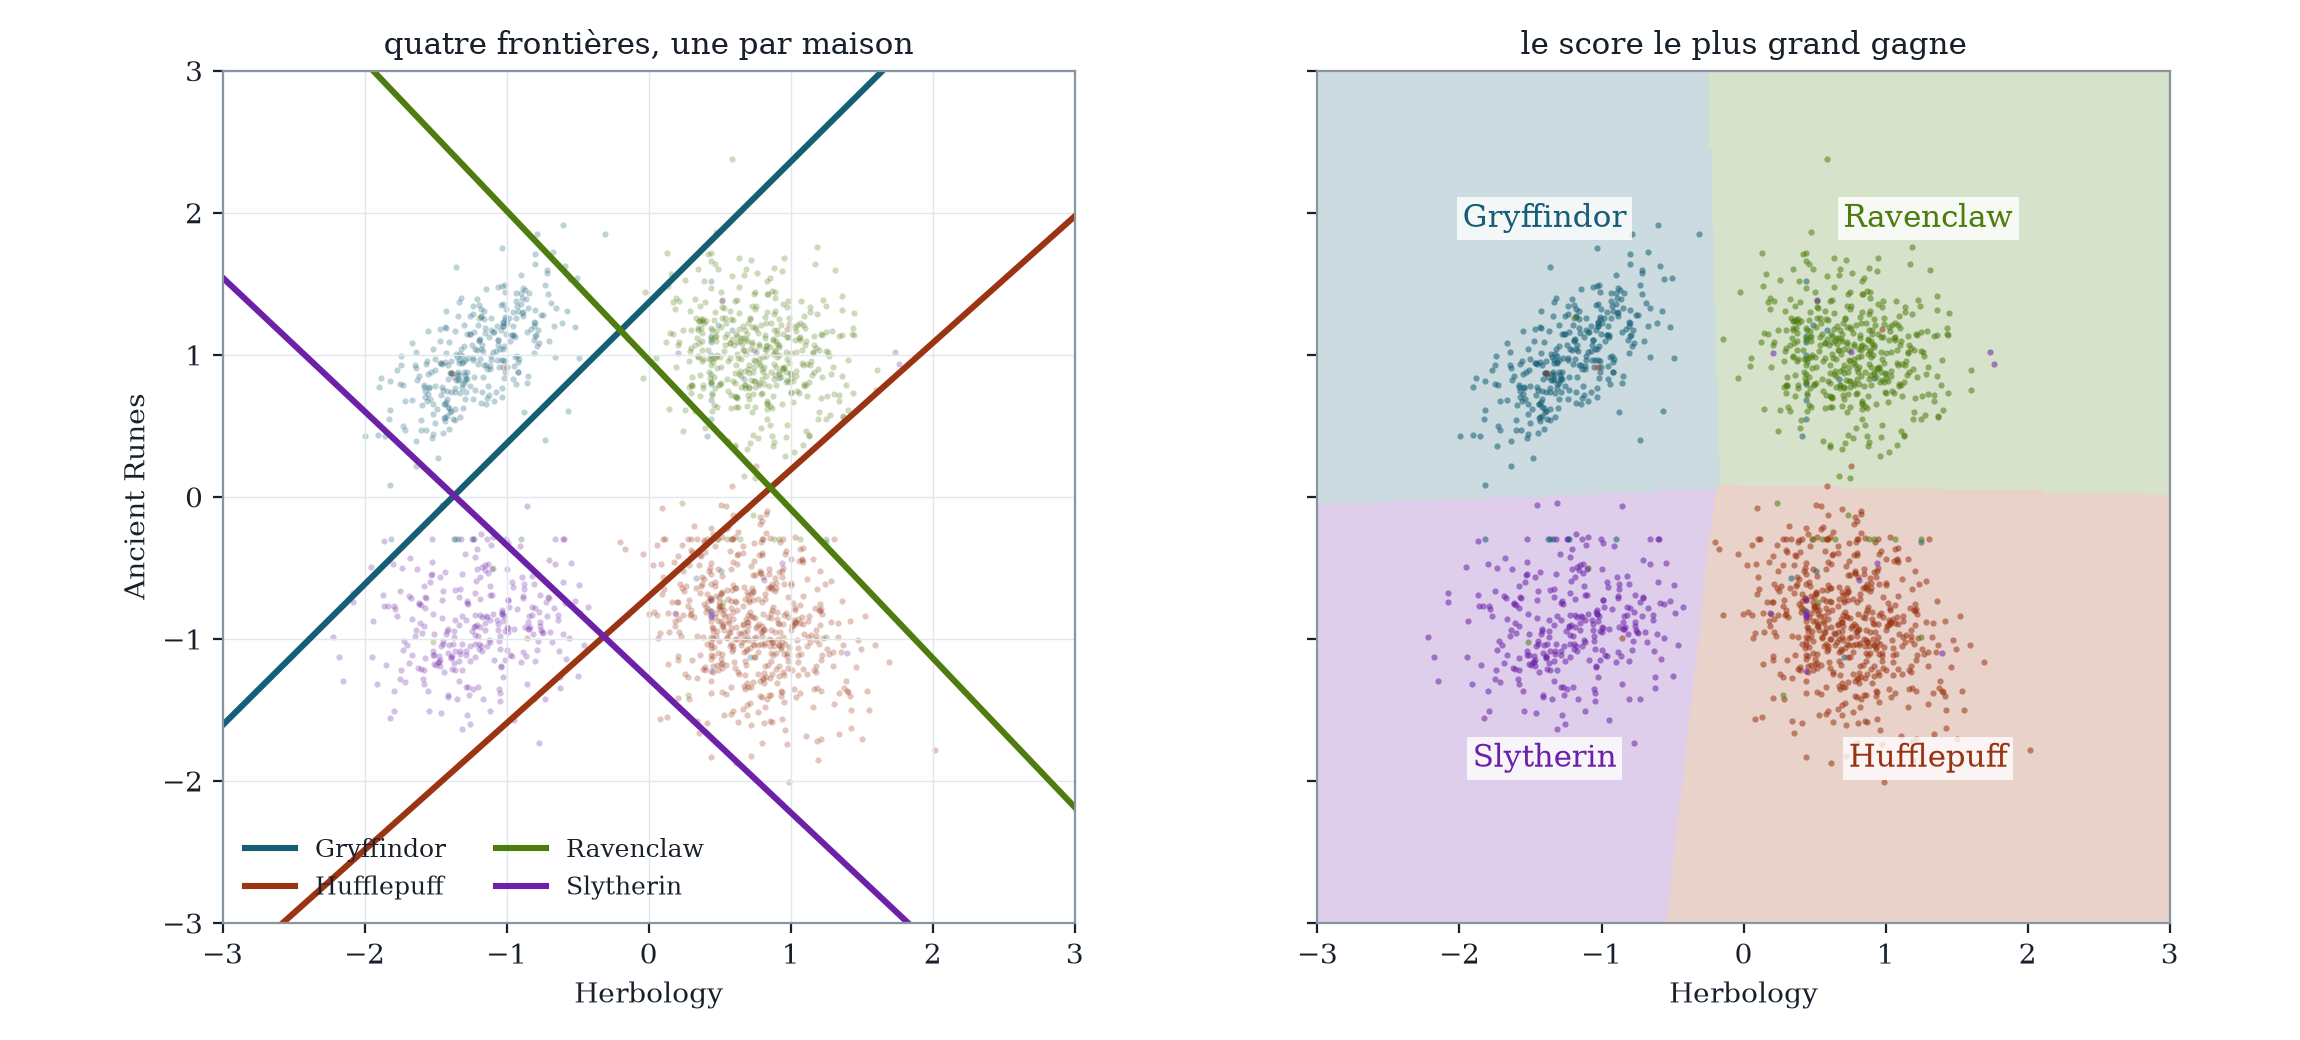
\includegraphics[width=\textwidth]{figures/regions_ovr.png}
\caption{À gauche, les quatre frontières, chacune séparant une maison des trois
autres. À droite, le découpage du plan qui en résulte : chaque point reçoit la
maison dont le score est le plus élevé. Les limites de ces quatre régions ont
leur propre direction, établie à la section suivante.}
\label{fig:regions}
\end{figure}
\FloatBarrier

\section{Forme des régions}

La règle du maximum attribue une maison à chaque point du plan. Quelle forme
prend alors l'ensemble des points attribués à une maison donnée ?

Prenons \Gryf. Son modèle l'emporte en un point lorsque son score y dépasse les
trois autres, ce qui fait trois conditions distinctes. La première s'écrit
\[
  z_G\geq z_H
  \iff
  (w_{G0}-w_{H0})+(w_{G1}-w_{H1})x_1+(w_{G2}-w_{H2})x_2\geq 0 ,
\]
et les deux autres s'obtiennent en remplaçant $H$ par $R$ puis par $S$. Le membre
de droite est une fonction affine des deux notes ; l'inégalité définit un
demi-plan, bordé par la droite où les deux scores s'égalisent.

\begin{figure}[htbp]
\centering
\makebox[\textwidth][c]{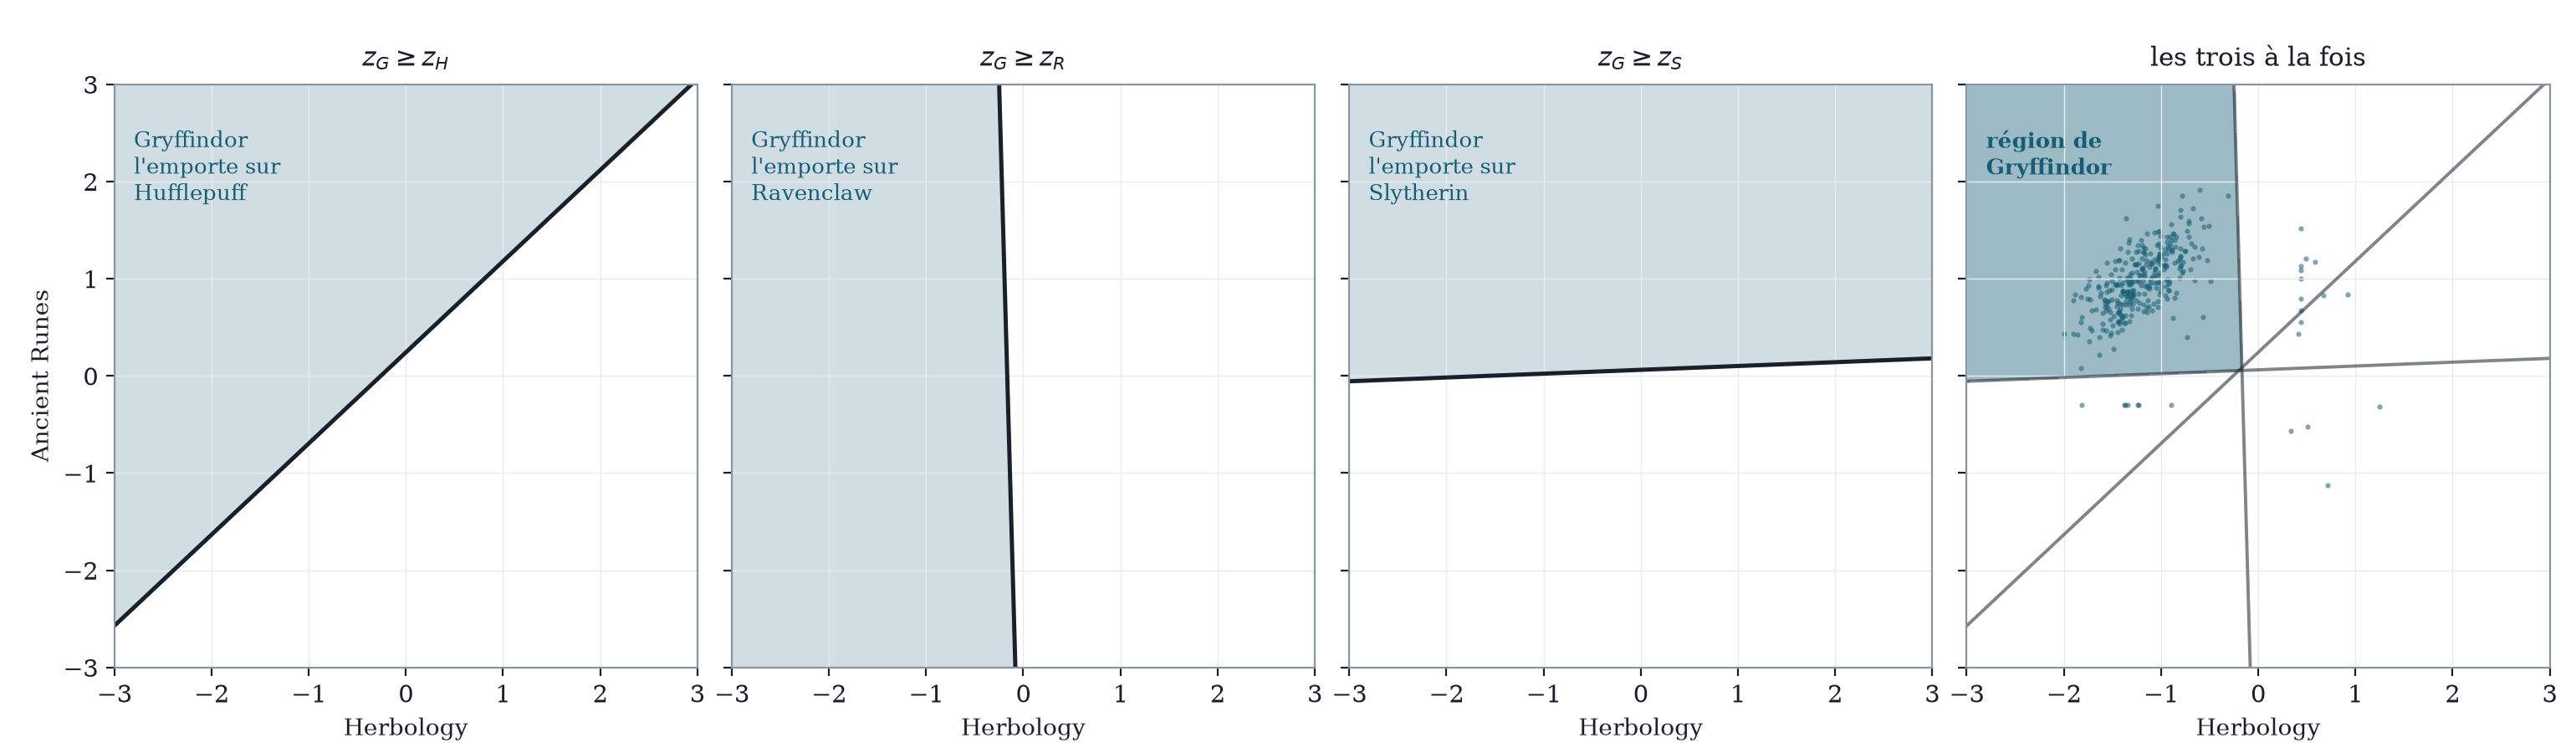
\includegraphics[width=1.18\textwidth]{figures/demiplans.png}}
\caption{Les trois demi-plans où \Gryf l'emporte sur chacun de ses rivaux, puis
leur intersection. Le dernier panneau porte les élèves de la maison, qui s'y
trouvent presque tous.}
\label{fig:demiplans}
\end{figure}
\FloatBarrier

La région de \Gryf est l'intersection de ces trois demi-plans, donc un polygone
convexe, éventuellement non borné. Trois propriétés en découlent directement.
Portés par les droites d'égalité $z_G=z_j$, ses bords se distinguent des quatre
frontières binaires du début de chapitre. Chacun s'interrompt là où un troisième
modèle prend le dessus, ce qui donne des arêtes de longueur finie. Et
deux élèves d'une même région ont tout le segment qui les joint dans cette
région, propriété de convexité qui interdit à une maison d'occuper deux zones
séparées.

Les quatre droites du début de chapitre ne disparaissent pas pour autant : la
droite $z_k=0$ sépare les points où le modèle $k$ répond « oui » de ceux où il
répond « non », tandis que la décision finale compare les quatre scores entre
eux. Ces deux questions sont différentes, et leurs droites aussi.

\begin{figure}[htbp]
\centering
\begin{tikzpicture}[x=1.28cm,y=1.28cm,font=\footnotesize]
\begin{scope}
\clip (-3,-3) rectangle (3,3);
\fill[gryff!7]  (-3,-3) -- (-0.082,-3) -- (-0.248,3) -- (-3,3) -- cycle;
\fill[raven!7]  (-0.082,-3) -- (3,-3) -- (3,3) -- (-0.248,3) -- cycle;
\draw[gridgray!35] (-3,-3) grid[step=1] (3,3);
\draw[gryff,very thick] (-3,-1.611) -- (3,4.343);
\draw[raven,very thick] (-3,4.114) -- (3,-2.186);
\draw[ink,ultra thick] (-0.082,-3) -- (-0.248,3);
\draw[ink,-{Stealth[length=2.4mm]},thick]
  (-0.197,1.171) -- ++(-0.99,-0.028);
\end{scope}
\draw[ink!45] (-3,-3) rectangle (3,3);
\draw[ink!45] (-3,0) -- (3,0);   \draw[ink!45] (0,-3) -- (0,3);
\fill[white] (-0.197,1.171) circle (2.1pt);
\draw[ink,thick] (-0.197,1.171) circle (2.1pt);
\node[gryff,anchor=west,fill=white,inner sep=1pt] at (-2.95,-1.95) {$z_G=0$};
\node[raven,anchor=east,fill=white,inner sep=1pt] at (2.95,-1.95) {$z_R=0$};
\node[ink,anchor=south,fill=white,inner sep=1.5pt] at (-0.16,3.02)
  {$z_G=z_R$};
\node[ink,anchor=south east,font=\scriptsize] at (-1.20,1.22)
  {$w_G-w_R$};
\node[gryff!85,anchor=west] at (-2.9,2.3) {$z_G>z_R$};
\node[raven!85,anchor=east] at (2.9,2.3) {$z_R>z_G$};
\node[anchor=north] at (0,-3.15) {\Herb};
\node[anchor=south,rotate=90] at (-3.15,0) {\Runes};
\end{tikzpicture}
\caption{Les deux frontières binaires de \Gryf et de \Rav, et la limite qui
sépare effectivement leurs deux régions. Cette limite a sa propre direction,
portée par le vecteur normal $w_G-w_R$, et passe par le point d'intersection des
deux premières : en ce point les deux scores valent $0$, donc ils sont égaux.}
\label{fig:limite-paire}
\end{figure}
\FloatBarrier

Quatre maisons forment six paires, donc six droites d'égalité, dont chacune ne
borde une région que sur la portion où le score commun aux deux maisons dépasse
aussi les deux autres. C'est la règle du maximum, et elle seule, qui attribue à
chaque point du plan exactement une maison, alors que les quatre modèles
s'ignorent.

Cette construction se vérifie le long d'un trajet : chaque score y devient une
fonction affine du chemin parcouru, donc une droite, et le maximum des quatre une
ligne brisée dont les points anguleux marquent les changements de région.

\begin{figure}[htbp]
\centering
\makebox[\textwidth][c]{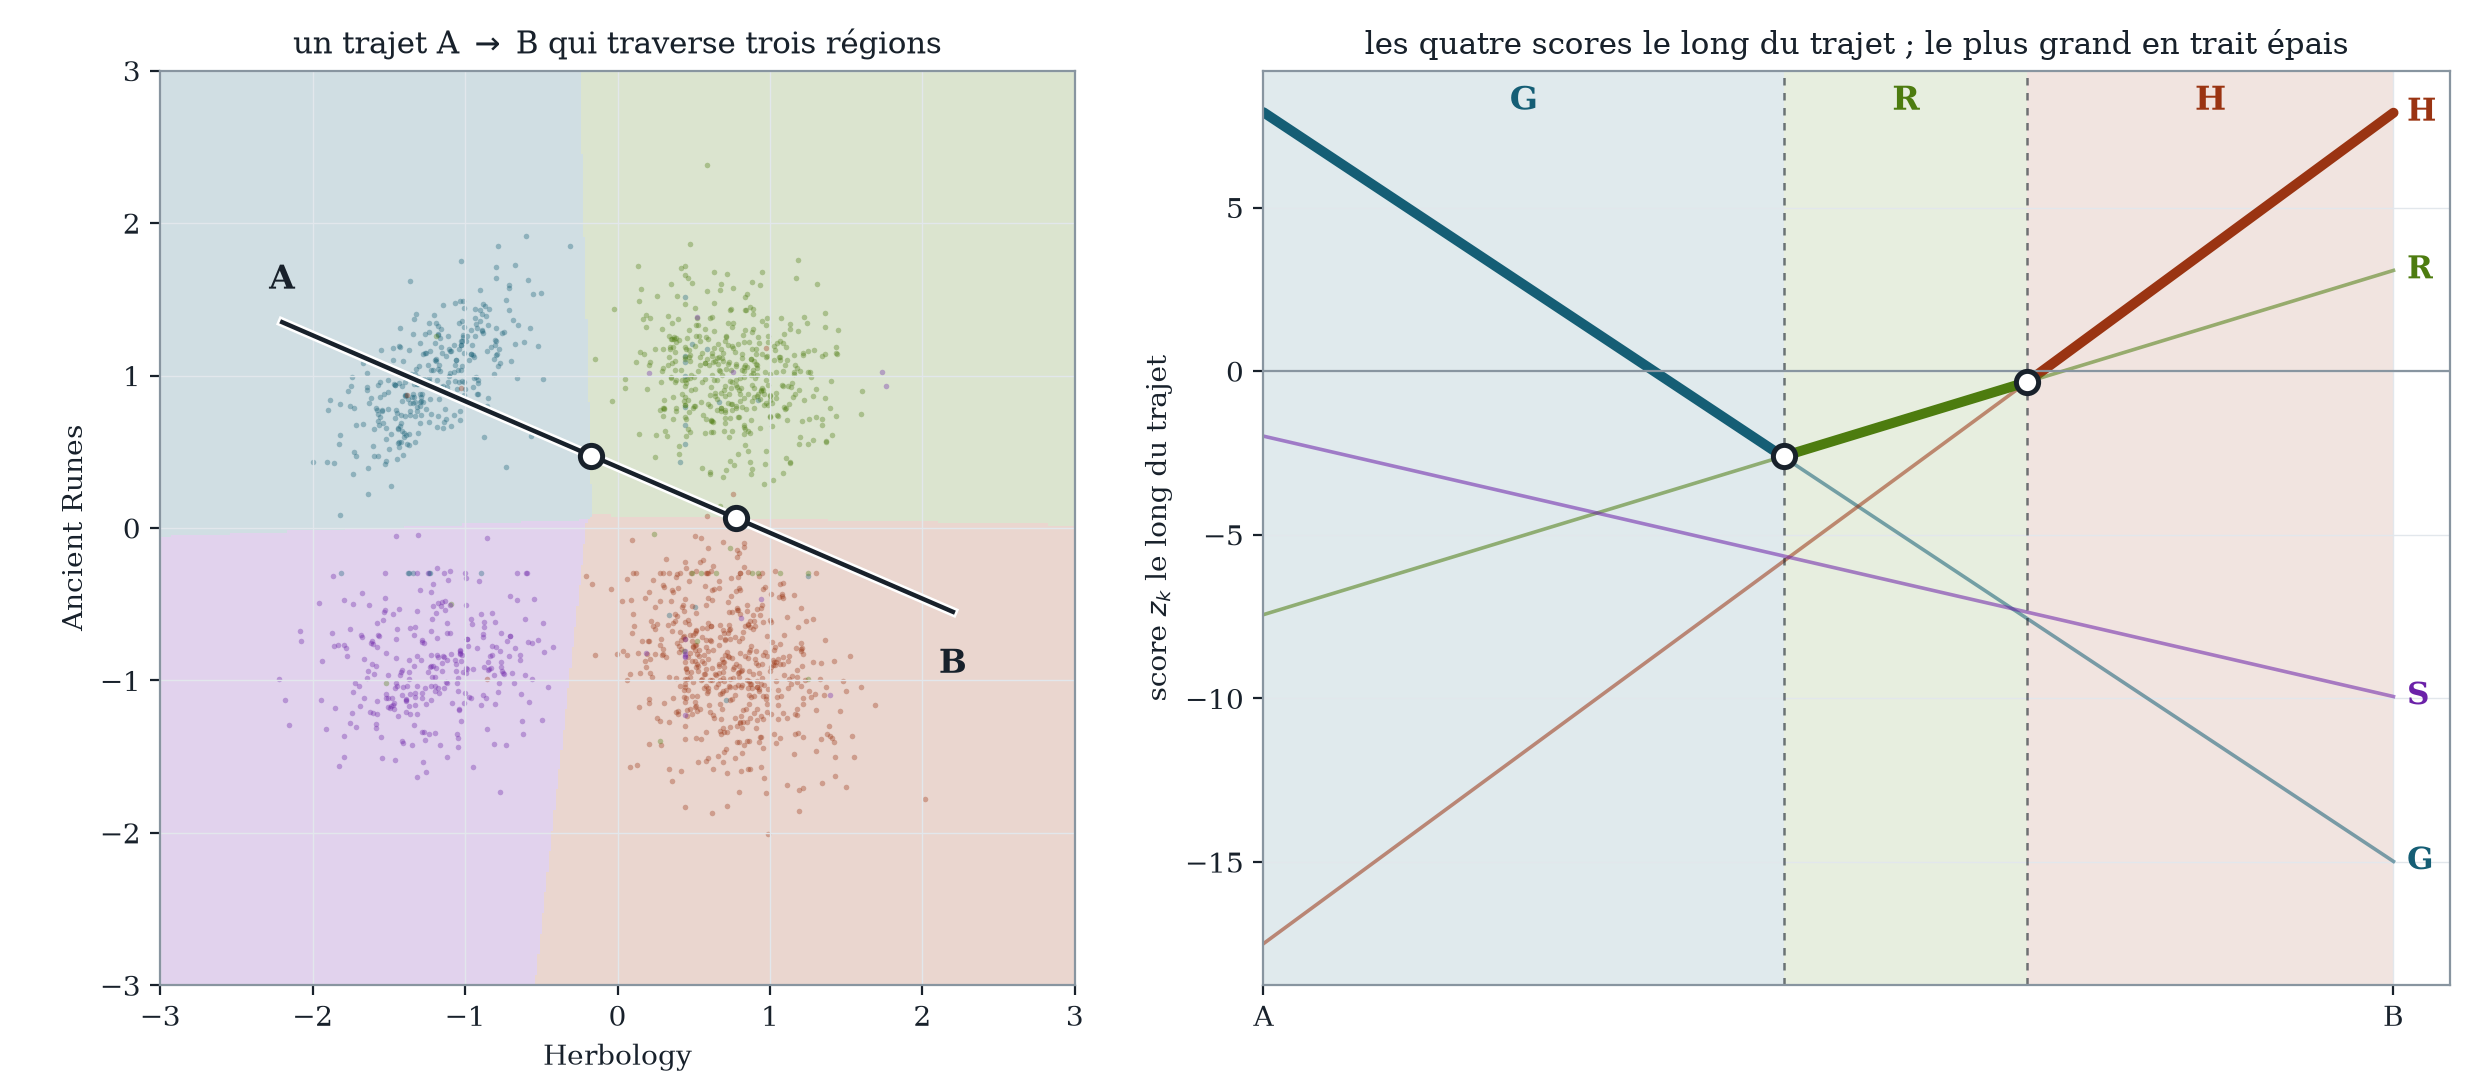
\includegraphics[width=1.2\textwidth]{figures/score_max.png}}
\caption{Le trajet du panneau de gauche part du groupe des \Gryf et rejoint celui
des \Huff. À droite, les quatre scores relevés le long de ce trajet. Le maximum
des quatre est la ligne brisée en trait épais : elle appartient à \Gryf sur le
premier tiers, à \Rav ensuite, à \Huff pour finir. Les deux points anguleux sont
les endroits où deux scores s'égalisent, et ce sont eux qui marquent le passage
d'une région à la suivante.}
\label{fig:score-max}
\end{figure}
\FloatBarrier
\section{Contenu du classifieur}

Avec dix matières au lieu de deux, chaque modèle a onze coefficients au lieu de
trois, sans autre modification. Le classifieur complet se réduit alors à :

\begin{figure}[htbp]
\centering
\begin{tikzpicture}[font=\footnotesize,
  cell/.style={draw=ink!25,minimum width=9mm,minimum height=5.4mm,
    font=\scriptsize,inner sep=1pt},
  head/.style={font=\scriptsize,text=ink,anchor=base},
  hname/.style={font=\scriptsize\bfseries,anchor=east}]

\foreach \r/\house/\col in {0/Gryffindor/gryff, 1/Hufflepuff/huffle,
                            2/Ravenclaw/raven, 3/Slytherin/slyth}{
  \node[hname,text=\col] at (-0.15,-0.62*\r) {\house};
  \node[cell,fill=\col!22] at (0.6,-0.62*\r) {$w_0$};
  \foreach \c in {1,2,3}{
    \node[cell,fill=\col!10] at (0.6+1.05*\c,-0.62*\r) {$w_{\c}$};
  }
  \node[font=\scriptsize,text=ink!60] at (4.9,-0.62*\r) {$\cdots$};
  \node[cell,fill=\col!10] at (5.85,-0.62*\r) {$w_{10}$};
}
\node[head] at (0.6,0.45) {biais};
\node[head] at (2.7,0.45) {une colonne par matière};

\draw[decorate,decoration={brace,amplitude=4pt},ink!45]
  (6.45,0.24) -- (6.45,-2.10);
\node[anchor=west,font=\scriptsize,text=ink,align=left] at (6.75,-0.93)
  {$4\times11=44$ coefficients,\\ plus $3\times10=30$ statistiques,\\
   plus deux listes ordonnées};
\end{tikzpicture}
\caption{Le classifieur complet, pour dix matières. Chaque ligne est un modèle
binaire indépendant, chaque colonne une matière ; la première colonne ne
correspond à aucune note. Les $44$ coefficients demandent leur contexte : les trois statistiques par
matière et l'ordre des lignes et des colonnes, faute de quoi ils s'appliquent à
des quantités inconnues.}
\label{fig:matrice-modele}
\end{figure}
\FloatBarrier

\begin{itemize}
  \item quatre vecteurs de onze coefficients, soit $44$ nombres ;
  \item la liste ordonnée des dix matières, qui dit à quelle note s'applique
        chaque coefficient ;
  \item la liste ordonnée des quatre maisons, qui dit quel vecteur correspond à
        quelle réponse ;
  \item pour chaque matière, la valeur d'imputation, la moyenne et l'écart-type
        appris à l'entraînement.
\end{itemize}

\begin{vigilance}[Ordre des colonnes et des maisons]
Un vecteur de coefficients s'applique aux notes dans l'ordre où il a été ajusté,
et l'indice du maximum ne devient une maison que par la liste des libellés.
Perdre l'un ou l'autre de ces ordres donne un classifieur qui calcule des scores
justes et rend des maisons fausses : une défaillance qui ne provoque aucune
erreur d'exécution.
\end{vigilance}

\section{Somme des quatre probabilités}

Chaque $\sigma(z_k)$ répond à sa propre question binaire : \emph{cet élève
est-il un \Gryf ?}, puis la même pour les trois autres maisons. Quatre expériences séparées, et donc quatre nombres libres les uns des autres, dont la
somme prend une valeur quelconque entre $0$ et $4$.

\begin{figure}[htbp]
\centering
\begin{tikzpicture}[y=3.4cm,font=\footnotesize]
% Trois eleves reels, quatre probabilites chacun (gen_sommes.py).
\draw[ink!35] (0,0) -- (12.4,0);
\draw[ink!30,densely dashed] (0,1) -- (12.4,1);
\node[anchor=east,font=\scriptsize,text=ink!70] at (-0.1,1) {$1$};
\node[anchor=east,font=\scriptsize,text=ink!70] at (-0.1,0) {$0$};
\foreach \g/\lab/\som in {0/{élève $1025$}/0.129, 4.4/{élève $326$}/1.021,
                          8.8/{élève $1067$}/1.845}{
  \node[anchor=north,font=\scriptsize,text=ink] at (\g+1.6,-0.03) {\lab};
  \node[anchor=north,font=\scriptsize\bfseries,text=ink]
    at (\g+1.6,-0.16) {somme $=\som$};
}
\foreach \x/\col/\p in {%
  0.4/gryff/0.003, 1.2/huffle/0.089, 2.0/raven/0.026, 2.8/slyth/0.010,
  4.8/gryff/0.007, 5.6/huffle/0.028, 6.4/raven/0.986, 7.2/slyth/0.000,
  9.2/gryff/0.949, 10.0/huffle/0.000, 10.8/raven/0.897, 11.6/slyth/0.000}{
  \fill[\col!70] (\x,0) rectangle (\x+0.55,\p);
  \draw[\col!45] (\x,0) rectangle (\x+0.55,\p);
}
\node[font=\scriptsize,text=gryff,anchor=south] at (9.48,0.96) {$0{,}949$};
\node[font=\scriptsize,text=raven,anchor=south] at (11.08,0.91) {$0{,}897$};
\node[font=\scriptsize,text=raven,anchor=south] at (6.68,0.99) {$0{,}986$};
\node[font=\scriptsize,text=huffle,anchor=south] at (1.48,0.10) {$0{,}089$};
\node[anchor=west,font=\scriptsize,text=ink!70] at (0,1.14)
  {\textcolor{gryff}{\Gryf} \quad \textcolor{huffle}{\Huff} \quad
   \textcolor{raven}{\Rav} \quad \textcolor{slyth}{\Slyth}};
\end{tikzpicture}
\caption{Les quatre probabilités de trois élèves du fichier, et leur somme. Le
premier reçoit moins de $0{,}09$ des quatre modèles, et sa maison est pourtant
correctement prédite : seul l'ordre compte. Le dernier dépasse $0{,}89$ pour deux
maisons à la fois. Sur les $1\,600$ élèves, la somme excède $1$ dans $981$ cas et
lui reste inférieure dans $619$.}
\label{fig:sommes}
\end{figure}
\FloatBarrier

La décision lit l'ordre de ces quatre nombres, et cet ordre reste valide quelle
que soit leur somme. Lire chacun d'eux comme une part d'un tout demanderait en
revanche que la somme vaille $1$ : c'est à cette condition qu'une phrase telle
que « $0{,}95$ de chances d'être \Gryf » prend son sens, et l'élève $1067$
montre où elle conduit ici, avec $0{,}949$ pour \Gryf et $0{,}897$ pour
\Rav. Le
modèle qui fournit directement une telle distribution est la régression softmax,
qui ajuste les quatre jeux de coefficients ensemble plutôt que séparément.

\begin{resultat}[Classifieur complet]
Quatre modèles binaires ajustés indépendamment sur les mêmes notes, et une
comparaison de leurs quatre scores. Sur \Herb et \Runes, cette règle
classe correctement $1\,540$ élèves sur $1\,600$ ; avec les dix matières du
fichier, elle dépasse $98\,\%$.
\end{resultat}


\part{Implémentation et évaluation}
\chapter{Écriture du score et du coût}
\label{ch:donnees}

\begin{lecture}
Le modèle est établi ; il reste à l'écrire, en Python et sans bibliothèque de
calcul. Quatre étapes mènent du score d'un seul élève au coût moyen sur les mille six
cents, chacune vérifiable par un nombre connu d'avance.
\end{lecture}

Le programme se répartit en neuf fichiers exécutables l'un après l'autre. Chacun
importe le précédent, ajoute une fonction, et affiche un nombre qui se contrôle
avant de passer au suivant.

\begin{figure}[htbp]
\centering
\begin{tikzpicture}[
  file/.style={draw=ink!30,rounded corners=2pt,font=\ttfamily\scriptsize,
    text width=40mm,align=left,inner xsep=5pt,inner ysep=3.4pt},
  what/.style={font=\small,text=ink,anchor=west},
  band/.style={rotate=90,font=\scriptsize\bfseries,align=center}]

\node[file,fill=accentlight] (f1) {step1\_score.py};
\node[file,fill=accentlight,below=2.4mm of f1] (f2) {step2\_sigmoid.py};
\node[file,fill=accentlight,below=2.4mm of f2] (f3) {step3\_single\_cost.py};
\node[file,fill=accentlight,below=2.4mm of f3] (f4) {step4\_total\_cost.py};
\node[file,fill=rulelight,below=2.4mm of f4] (f5) {step5\_gradient.py};
\node[file,fill=rulelight,below=2.4mm of f5] (f6) {step6\_one\_step.py};
\node[file,fill=rulelight,below=2.4mm of f6] (f7) {step7\_loop.py};
\node[file,fill=warninglight,below=2.4mm of f7] (f8) {step8\_four\_houses.py};
\node[file,fill=warninglight,below=2.4mm of f8] (f9) {step9\_holdout.py};

\node[what,right=4mm of f1] {le score d'un élève};
\node[what,right=4mm of f2] {la sigmoïde, écrite pour ne pas déborder};
\node[what,right=4mm of f3] {le coût d'une prédiction};
\node[what,right=4mm of f4] {la lecture du fichier, le coût moyen};
\node[what,right=4mm of f5] {la pente, et sa vérification par mesure};
\node[what,right=4mm of f6] {un pas de descente};
\node[what,right=4mm of f7] {la boucle et ses deux arrêts};
\node[what,right=4mm of f8] {quatre descentes, le plus grand score};
\node[what,right=4mm of f9] {l'exactitude hors des élèves appris};

\fill[accent!16,rounded corners=1.5pt]
  ($(f1.north west)+(-9mm,0)$) rectangle ($(f4.south west)+(-4mm,0)$);
\fill[rulecolor!16,rounded corners=1.5pt]
  ($(f5.north west)+(-9mm,0)$) rectangle ($(f7.south west)+(-4mm,0)$);
\fill[warning!16,rounded corners=1.5pt]
  ($(f8.north west)+(-9mm,0)$) rectangle ($(f9.south west)+(-4mm,0)$);
\node[band,text=accent]
  at ($(f1.north west)!0.5!(f4.south west)+(-6.5mm,0)$) {le coût};
\node[band,text=rulecolor]
  at ($(f5.north west)!0.5!(f7.south west)+(-6.5mm,0)$) {la descente};
\node[band,text=warning]
  at ($(f8.north west)!0.5!(f9.south west)+(-6.5mm,0)$) {les maisons};
\end{tikzpicture}
\caption{Les cinq derniers fichiers importent tous \texttt{step4}, dont
\texttt{load} et \texttt{total\_cost} servent jusqu'à la dernière étape.}
\label{fig:montage}
\end{figure}
\FloatBarrier

\section{Étape 1 : le score d'un élève}

Le score est une somme de trois produits. Les deux notes arrivent déjà
standardisées, opération traitée à l'étape~4, et les trois coefficients valent
zéro.

\codefile{scripts/tuto/step1_score.py}

\begin{console}
score: 0.0
\end{console}

Le $1{,}0$ en tête de \texttt{x} vaut $1$ pour tous les élèves : c'est la colonne
du biais, qui fait entrer \texttt{weights[0]} dans la somme sans le multiplier par
une donnée. Sans elle, chaque formule ultérieure devrait traiter
\texttt{weights[0]} à part, y compris celle de la pente.

Des coefficients nuls donnent un score nul pour n'importe quel élève. La sortie
ne contrôle donc que la mécanique de la somme.

\section{Étape 2 : la probabilité}

Le score parcourt tout $\R$, la probabilité doit tomber entre $0$ et $1$. La
fonction logistique opère ce passage (ch.~\ref{ch:logit}).

\codefile[firstline=4,lastline=7]{scripts/tuto/step2_sigmoid.py}

Les deux branches calculent la même valeur et diffèrent par le seul exposant
employé. En double précision, $e^{u}$ dépasse le plus grand flottant
représentable dès $u>709{,}78$ : l'écriture $1/(1+e^{-z})$ échoue donc pour tout
score inférieur à $-710$, alors que la valeur cherchée est simplement $0$.
Multiplier haut et bas par $e^{z}$ donne $e^{z}/(1+e^{z})$, dont l'exposant reste
négatif de ce côté : $e^{-800}$ passe sous le plus petit flottant, vaut $0$ sans
lever d'exception, et le quotient rend $0$.

\begin{console}
sigmoid(0)    = 0.5
sigmoid(2)    = 0.8808
sigmoid(-800) = 0.0
single branch : OverflowError, math range error
\end{console}

La dernière ligne exécute l'écriture à une seule branche sur le même nombre. Un
score de $-800$ apparaît dès qu'un coefficient diverge
(ch.~\ref{ch:convexite}).

\begin{vigilance}[Contrôle en zéro]
$\sigma(0)$ vaut $0{,}5$ exactement. Une fonction qui rend autre chose en zéro
est fausse, et tout ce qui la suit le sera.
\end{vigilance}

\section{Étape 3 : le coût d'un élève}

Le modèle annonce une probabilité, le fichier donne la réponse observée. Le coût
mesure l'écart entre les deux.

\codefile[firstline=5,lastline=8]{scripts/tuto/step3_single_cost.py}

Les deux termes ne servent jamais ensemble : \texttt{expected} annule l'un et
conserve l'autre.

\begin{figure}[htbp]
\centering
\begin{tikzpicture}[
  case/.style={rounded corners=2.5pt,inner sep=7pt,align=center,font=\small,
    text width=66mm},
  tag/.style={font=\footnotesize\bfseries,anchor=south},
  note/.style={font=\footnotesize,text=ink,align=center,text width=66mm}]
\node[case,fill=accentlight,draw=accent!55] (a)
  {$-\bigl[\,{\color{accent}1\cdot\log p}\;+\;{\color{ink!22}0\cdot\log(1-p)}\,\bigr]$};
\node[case,fill=warninglight,draw=warning!55,right=4mm of a] (b)
  {$-\bigl[\,{\color{ink!22}0\cdot\log p}\;+\;{\color{warning}1\cdot\log(1-p)}\,\bigr]$};
\node[tag,text=accent,above=1.2mm of a] {\texttt{expected = 1.0}};
\node[tag,text=warning,above=1.2mm of b] {\texttt{expected = 0.0}};
\node[note,below=1.2mm of a] {l'élève est dans la maison\\ le coût vaut $-\log p$};
\node[note,below=1.2mm of b] {l'élève est ailleurs\\ le coût vaut $-\log(1-p)$};
\end{tikzpicture}
\caption{Le facteur nul annule son terme avant que le logarithme ne soit
évalué ; aucune des deux branches ne calcule $\log 0$ tant que $p$ reste
strictement entre $0$ et $1$, ce que garantit la sigmoïde.}
\label{fig:deux-cas}
\end{figure}
\FloatBarrier

\begin{console}
no opinion, student inside the house  : 0.693147
no opinion, student outside           : 0.693147
confident and right                   : 0.002476
confident and wrong                   : 6.002476
log(2) = 0.693147
\end{console}

Les deux premières lignes correspondent à $z=0$, donc $p=0{,}5$ : le coût vaut
$\log 2$ quelle que soit la réponse attendue, puisque les deux termes sont alors
symétriques. Pour les deux suivantes, $z=6$ et $p=0{,}9975$. Cette probabilité coûte $0{,}0025$ lorsqu'elle porte sur la réponse observée et
$6{,}0025$ lorsqu'elle porte sur l'autre : pour une prédiction fausse assortie
d'un score élevé, le coût croît comme $|z|$, sans borne supérieure.

\section{Étape 4 : le coût moyen}

Deux traitements précèdent l'emploi des notes brutes.

\codefile[firstline=15,lastline=21]{scripts/tuto/step4_total_cost.py}

\Herb compte $33$ notes absentes et \Runes $35$, sur $1\,600$ lignes.
Elles reçoivent la médiane de leur colonne plutôt que la moyenne : quelques notes
extrêmes déplacent la seconde et non la première.

Les deux colonnes n'ont ensuite ni le même centre ni la même dispersion.
\Herb a pour moyenne $1{,}19$ et pour écart-type $5{,}18$, \Runes
$495{,}05$ et $105{,}19$. Un même coefficient produirait donc dans la seconde un
effet vingt fois plus grand que dans la première, pour une raison qui tient à
l'unité de la note et non à ce qu'elle dit de l'élève. Après retrait de la
moyenne et division par l'écart-type, les deux colonnes ont pour moyenne $0$ et
pour écart-type $1$, et un coefficient de $3$ signifie la même chose des deux
côtés.

\codefile[firstline=24,lastline=30]{scripts/tuto/step4_total_cost.py}

\begin{figure}[htbp]
\centering
\begin{tikzpicture}[
  tab/.style={draw=ink!30,rounded corners=2pt,fill=white,inner sep=5pt},
  arr/.style={-{Latex[length=2.2mm]},thick,ink!65},
  op/.style={font=\scriptsize,text=ink,align=center},
  head/.style={font=\scriptsize\bfseries,text=ink,anchor=south}]

\node[tab] (brut) {\footnotesize\begin{tabular}{r@{\hskip 4mm}r}
\textcolor{herbo}{Herbo.} & \textcolor{runes}{A.\ Runes}\\[1pt]
$-6{,}497$ & $523{,}982$\\
$-7{,}82$ & $599{,}33$\\
$-5{,}76$ & \textcolor{warning}{absente}\\
$+5{,}73$ & $532{,}48$\\
\end{tabular}};

\node[tab,right=26mm of brut] (std) {\footnotesize\begin{tabular}{r@{\hskip 3mm}r@{\hskip 3mm}r}
$1{,}000$ & $-1{,}485$ & $+0{,}275$\\
$1{,}000$ & $-1{,}741$ & $+0{,}991$\\
$1{,}000$ & $-1{,}344$ & \textcolor{warning}{$-0{,}296$}\\
$1{,}000$ & $+0{,}877$ & $+0{,}356$\\
\end{tabular}};

\node[head,above=1.5mm of brut] {le fichier};
\node[head,above=1.5mm of std] {\texttt{X}};
\draw[arr] (brut) -- node[op,above=0.5mm]{médiane,\\puis $(v-\mu)/\sigma$} (std);
\node[op,below=1.5mm of brut] {quatre élèves parmi $1\,600$};
\node[op,below=1.5mm of std] {la première colonne vaut $1$ partout};
\end{tikzpicture}
\caption{La médiane d'\Runes, $463{,}92$, remplace la note absente du
troisième élève et donne $-0{,}296$ après standardisation. Sa ligne reste
exploitable.}
\label{fig:matrice}
\end{figure}
\FloatBarrier

Le coût moyen se calcule alors élève par élève, en réutilisant les deux fonctions
précédentes.

\codefile[firstline=33,lastline=44]{scripts/tuto/step4_total_cost.py}

\begin{figure}[htbp]
\centering
\begin{tikzpicture}[
  val/.style={draw=ink!35,rounded corners=2.5pt,fill=white,font=\small,
    align=center,inner sep=5pt,minimum width=22mm,minimum height=9mm},
  fn/.style={font=\ttfamily\scriptsize,text=accent,align=center},
  arr/.style={-{Latex[length=2mm]},thick,ink!65},
  side/.style={font=\ttfamily\scriptsize,text=ink,align=center},
  drop/.style={-{Latex[length=1.8mm]},ink!45}]
\node[val] (x) {$x$};
\node[val,right=20mm of x] (z) {$z=0{,}000$};
\node[val,right=20mm of z] (p) {$p=0{,}500$};
\node[val,right=20mm of p] (c) {$0{,}693147$};
\coordinate (m1) at ($(x)!0.5!(z)$);
\coordinate (m3) at ($(p)!0.5!(c)$);
\draw[arr] (x) -- node[fn,above=0.8mm]{score\_of} (z);
\draw[arr] (z) -- node[fn,above=0.8mm]{sigmoid} (p);
\draw[arr] (p) -- node[fn,above=0.8mm]{student\_cost} (c);
\node[side,above=9mm of m1] (w) {weights\\ $(0,0,0)$};
\node[side,above=9mm of m3] (e) {expected\\ $=1$};
\draw[drop] (w) -- (m1);
\draw[drop] (e) -- (m3);
\node[side,below=1.5mm of x] {$[1{,}0\;\;{-}1{,}485\;\;0{,}275]$};
\end{tikzpicture}
\caption{L'élève $3$ traversant les trois fonctions, coefficients nuls. Les
coefficients n'interviennent qu'au premier passage et la réponse attendue qu'au
dernier : entre les deux, le calcul ne dépend plus des données.}
\label{fig:circuit}
\end{figure}
\FloatBarrier

\begin{console}
1600 students, 3 columns (bias included)
cost with zero weights: 0.693147
\end{console}

\begin{resultat}[Contrôle de sortie]
Sur des coefficients nuls, le programme doit afficher $0{,}693147$
(ch.~\ref{ch:erreur}). Cette valeur est la même pour tout fichier, tout choix de
matières et tout nombre d'élèves : un écart localise donc l'erreur dans le score,
la sigmoïde ou le coût.
\end{resultat}

Le programme sait maintenant juger un jeu de coefficients. En produire un
meilleur est l'objet du chapitre suivant.

% !TeX root = ../regression_logistique.tex
\chapter{Optimisation des coefficients}
\label{ch:entrainer}

\orient{%
écrire le gradient et le contrôler contre une mesure par différences finies ;
écrire un pas ; écrire une boucle dont le critère d'arrêt teste une baisse et
rend des coefficients cohérents avec la perte retournée}{%
chapitre~\ref{ch:donnees} ; \annexeref{ann:gradient}}{%
cahier pratique}

Un jeu de coefficients étant évalué, trois étapes séparent ce point d'une boucle
d'entraînement : la direction du déplacement, sa vérification, puis son
itération.

\section{La pente et sa vérification}

La pente du coût par rapport à chaque coefficient s'obtient par une formule
démontrée à l'\annexeref{ann:gradient}. Les trois pentes sortent ensemble d'un
seul passage sur les observations.

Une erreur de signe ou un indice décalé produit ici un programme qui s'exécute,
converge lentement et reste silencieux. La formule se contrôle sans
démonstration, en mesurant ce qu'elle prétend calculer : une pente est un rapport
d'accroissements, obtenu en déplaçant un coefficient dans les deux sens et en
divisant l'écart de coût par la distance parcourue.

\begin{tache}{Gradient et contrôle numérique}
\tlab{Contrat} \texttt{gradient(weights, X, target)} rend la liste des
$\partial J/\partial w_j$, calculée en un seul passage sur \texttt{X}.
\texttt{measured\_slope(weights, X, target, j, h)} rend la même dérivée par
différence centrée, en appelant deux fois \texttt{total\_cost}.

\tlab{Contrôle} En $(0{,}3\,;-0{,}7\,;0{,}4)$ et $h=10^{-5}$ :
\begin{center}\ttfamily\footnotesize
\begin{tabular}{@{}rrr@{}}
colonne & formule & mesure\\
0 & +0.358202569 & +0.358202569\\
1 & +0.071184453 & +0.071184453\\
2 & -0.098350181 & -0.098350181\\
\end{tabular}
\end{center}
Écart attendu : de l'ordre de $10^{-10}$.

\tlab{Indice 1} La formule est
$\frac{1}{m}\sum_i (p_i-y_i)\,x_{ij}$ : accumuler un résidu par ligne, puis le
répartir sur les colonnes de cette ligne.

\tlab{Indice 2} \texttt{measured\_slope} ignore tout de la régression
logistique : elle déplace \texttt{weights[j]} de $\pm h$, rappelle
\texttt{total\_cost}, et divise par $2h$.

\tlab{Transfert} Le point d'évaluation est choisi loin de zéro. Montrer qu'en
$(0,0,0)$ un facteur $1/m$ omis passerait inaperçu, et proposer un second point
de contrôle qui révélerait un indice décalé.
\corrige{step5\_gradient.py}
\end{tache}

\begin{figure}[htbp]
\centering
\begin{graphique}{Un bloc d'entrée se sépare en deux chemins : à gauche la fonction gradient, un passage sur les observations ; à droite measured_slope, deux coûts complets. Les deux convergent vers un bloc de comparaison indiquant que les valeurs coïncident sur neuf décimales.}
\begin{tikzpicture}[
  box/.style={rounded corners=2.5pt,inner sep=6pt,align=center,font=\small,
    text width=62mm,draw=ink!30},
  arr/.style={-{Latex[length=2mm]},thick,ink!60}]
\node[box,fill=gridgray!20] (in)
  {\texttt{weights} $=(0{,}3\,;-0{,}7\,;0{,}4)$\\ \texttt{X}, \texttt{target}};
\node[box,fill=accentlight,below=11mm of in,xshift=-34mm] (form)
  {\texttt{gradient}\\[2pt] la formule,\\ un passage sur les observations};
\node[box,fill=rulelight,below=11mm of in,xshift=34mm] (mes)
  {\texttt{measured\_slope}\\[2pt] deux coûts complets,\\ déplacement de $\pm10^{-5}$};
\coordinate (mid) at ($(form.south)!0.5!(mes.south)$);
\node[box,fill=white,draw=ink!45,below=10mm of mid,text width=100mm] (cmp)
  {les deux valeurs coïncident sur neuf décimales,\\ aux trois colonnes};
\draw[arr] (in) -- (form);
\draw[arr] (in) -- (mes);
\draw[arr] (form) -- (cmp);
\draw[arr] (mes) -- (cmp);
\end{tikzpicture}
\end{graphique}
\caption{Deux chemins indépendants vers la même dérivée. Le point d'évaluation
est choisi loin de zéro, où plusieurs erreurs classiques rendent zéro des deux
côtés.}
\label{fig:controle-gradient}
\end{figure}
\FloatBarrier

L'écart résiduel vient de la mesure. Centrée sur un pas $h$, une différence
commet une erreur en $h^2$, soit $10^{-10}$ pour $h=10^{-5}$, ce que les trois
lignes retrouvent. Un $h$ plus grand mesurerait une corde au lieu d'une tangente ;
un $h$ plus petit ferait perdre à la soustraction ses décimales significatives.

\begin{vigilance}[Ordre de grandeur de l'écart]
Un écart de l'ordre de $10^{-10}$ valide la formule. Un écart de $10^{-2}$
désigne un facteur oublié, un signe opposé désigne une soustraction inversée, et
une seule colonne fausse désigne l'indice.
\end{vigilance}

\section{Un pas}

Descendre consiste à retrancher la pente, multipliée par la longueur du pas.

\begin{tache}{Un pas de descente}
\tlab{Contrat} \texttt{one\_step(weights, X, target)} rend une \emph{nouvelle}
liste de coefficients, chacun diminué de \texttt{ALPHA} fois sa dérivée.

\tlab{Contrôle} À partir de coefficients nuls et $\alpha=1$ :
\begin{center}\ttfamily\footnotesize
\begin{tabular}{@{}llll@{}}
turn 0 & cost 0.693147 & weights & +0.0000 +0.0000 +0.0000\\
turn 1 & cost 0.538507 & weights & -0.2956 -0.2289 +0.1924\\
turn 2 & cost 0.449297 & weights & -0.5194 -0.4005 +0.3364\\
turn 3 & cost 0.393020 & weights & -0.6955 -0.5348 +0.4500\\
\end{tabular}
\end{center}
Le premier biais, $-0{,}2956$, se recalcule à la main : voir ci-dessous.

\tlab{Indice 1} Construire la liste neuve plutôt que modifier en place.
Corriger \texttt{weights[0]} avant de calculer la correction de
\texttt{weights[1]} évaluerait les deux pentes en deux points différents.

\tlab{Indice 2} Le signe est un moins : on se déplace à l'opposé de la pente.
Si le coût monte au premier tour, la cause est le signe ou la valeur d'\texttt{ALPHA}.

\tlab{Transfert} Prédire, sans exécuter, le signe de $w_1$ et de $w_2$ après le
premier tour, à partir de la position des \Gryf dans le nuage
(figure~\ref{fig:nuage}).
\corrige{step6\_one\_step.py}
\end{tache}

Les coefficients étant nuls, le modèle produit $0{,}5$ pour les $1\,600$ lignes,
et la pente du biais vaut la moyenne des résidus $\sigma(z)-y$, où $y$ vaut $1$
pour les \Gryf et $0$ pour les autres.

\begin{figure}[htbp]
\centering
\begin{graphique}{Une barre horizontale partagée en deux : un segment bleu de 327 Gryffindor à gauche, un segment gris de 1273 élèves des autres maisons à droite. Sous chaque segment, le résidu correspondant, -0,5 et +0,5, puis le calcul de leur moyenne pondérée, égale à 0,2956.}
\begin{tikzpicture}[font=\small]
\fill[accent!65] (0,0) rectangle (2.45,0.72);
\fill[gridgray!45] (2.45,0) rectangle (12,0.72);
\draw[ink!35] (0,0) rectangle (12,0.72);
\node[font=\footnotesize\bfseries,text=white] at (1.22,0.36) {$327$};
\node[font=\footnotesize,text=ink] at (7.2,0.36)
  {$1\,273$ élèves des trois autres maisons};
\node[anchor=south,font=\footnotesize,text=accent] at (1.22,0.78)
  {\Gryf, $20{,}44\,\%$};
\node[anchor=north,font=\footnotesize,text=accent] at (1.22,-0.12)
  {$\sigma(0)-1=-0{,}5$};
\node[anchor=north,font=\footnotesize,text=ink] at (7.2,-0.12)
  {$\sigma(0)-0=+0{,}5$};
\node[anchor=north,font=\small] at (6,-1.05)
  {moyenne $=\dfrac{1\,273\times0{,}5-327\times0{,}5}{1\,600}=0{,}2956$};
\end{tikzpicture}
\end{graphique}
\caption{Le pas retranche cette moyenne au biais, d'où $-0{,}2956$ au premier
tour : le biais rejoint la valeur qui fait annoncer $20{,}44\,\%$ à toutes les
observations.}
\label{fig:premierpas}
\end{figure}
\FloatBarrier

\section{Itération jusqu'à stagnation}

Un pas isolé fait baisser la perte d'une fraction. La descente répète ce pas
jusqu'à ce que la baisse devienne négligeable, ce qui demande une boucle et deux
conditions d'arrêt.

\begin{tache}{La boucle et ses deux arrêts}
\tlab{Contrat} \texttt{descend(X, target)} rend le couple
\texttt{(weights, cost)} correspondant au même état, ainsi que le nombre de tours
consommés. La boucle s'arrête sur une baisse relative inférieure à
\texttt{EPSILON} $=10^{-6}$, ou sur un plafond de $6\,000$ tours.

\tlab{Contrôle}
\begin{center}\ttfamily\footnotesize
stopped after 983 iterations, cost 0.107257\\
weights: -5.1755 -3.7460 +3.7874
\end{center}
Le nombre d'itérations se lit en premier : à $983$ pour un plafond de $6\,000$,
c'est le critère de stagnation qui a mis fin à la boucle. Une valeur égale au
plafond signalerait un pas trop court, ou l'absence de minimum fini
(\annexeref{ann:norme}).

\tlab{Indice 1} Le test doit porter sur \texttt{previous - cost}, une baisse, et
non sur \texttt{abs(previous - cost)}.

\tlab{Indice 2} Appliquer le pas \emph{avant} de calculer la perte retournée :
les deux valeurs décrivent alors le même état.

\tlab{Transfert} Le seuil relatif $10^{-6}$ est atteint après $983$ tours, alors
que la frontière a cessé de se déplacer bien avant (ch.~\ref{ch:descente}).
Proposer un critère d'arrêt qui testerait la stabilité des \emph{décisions}, et
dire ce qu'il coûterait par tour.
\corrige{step7\_loop.py}
\end{tache}

\begin{vigilance}[Trois pièges du critère d'arrêt]
\textbf{Valeur absolue.} Écrire \texttt{abs(previous - cost) < seuil} accepte
aussi une hausse faible de la perte et peut donc arrêter à tort une boucle
instable.

\textbf{Relatif ou absolu.} Écrire \texttt{... / max(1, abs(cost))} ne
normalise pas le coût lorsqu'il est inférieur à $1$. La forme
\texttt{previous - cost < EPSILON * abs(previous)} conserve une interprétation
relative.

\textbf{Cohérence entre retours.} La perte et les coefficients retournés
doivent décrire le même état ; appliquer un pas après le dernier calcul de perte
les décale d'une itération.
\end{vigilance}

\begin{figure}[htbp]
\centering
\begin{graphique}{Trois blocs empilés reliés en boucle : total_cost, gradient, one_step, la sortie de one_step revenant sur total_cost avec la mention au plus 6000 tours. Une flèche latérale sort de total_cost vers le retour des coefficients et du coût, sous condition d'une baisse relative inférieure à 10 puissance -6.}
\begin{tikzpicture}[
  st/.style={draw=ink!30,rounded corners=2.5pt,align=center,font=\small,
    inner sep=6pt,text width=34mm},
  lab/.style={font=\footnotesize,text=ink,align=left},
  arr/.style={-{Latex[length=2mm]},thick,ink!60}]
\node[st,fill=accentlight] (c) {\texttt{total\_cost}};
\node[st,fill=rulelight,below=13mm of c] (g) {\texttt{gradient}};
\node[st,fill=warninglight,below=13mm of g] (u) {\texttt{one\_step}};
\node[st,fill=white,draw=accent!60,left=16mm of c] (out)
  {\texttt{return}\\ \texttt{weights, cost}};
\coordinate (ret) at ($(u.east)+(12mm,0)$);
\draw[arr] (c) -- (g);
\draw[arr] (g) -- (u);
\draw[arr] (u.east) -- (ret) |- (c.east);
\node[lab,right=1mm of ret,text width=26mm] {au plus\\ $6\,000$ tours};
\draw[arr] (c) -- node[lab,above=1mm,align=center]
  {baisse relative\\ sous $10^{-6}$} (out);
\end{tikzpicture}
\end{graphique}
\caption{Le coût est calculé une fois par tour, pour le seul test d'arrêt. Le
gradient constitue un second passage sur les $1\,600$ lignes : une itération en
coûte deux.}
\label{fig:boucle}
\end{figure}
\FloatBarrier

Le seuil relatif arrête les itérations lorsque la baisse du coût devient
négligeable. Le plafond couvre les configurations où les coefficients divergent
et où ce seuil n'est jamais atteint (\annexeref{ann:norme}).

Ces coefficients constituent l'état \Mstop. Les figures de la partie~I emploient
\Mquatre, arrêté au quatre-centième tour : $-4{,}745$, $-3{,}454$, $+3{,}469$.
Les deux états diffèrent d'environ $9\,\%$ en norme, et leurs rapports coïncident
à trois millièmes près : la frontière se stabilise avant la perte, tandis que
les derniers tours resserrent la sigmoïde.

% !TeX root = ../regression_logistique.tex
\chapter{Classification multiclasse et évaluation}
\label{ch:predire}

\orient{%
appliquer la même descente aux quatre classes et combiner les résultats par
argmax ; construire un découpage stratifié ; ajuster les statistiques de
préparation sur l'apprentissage seul ; lire une matrice de confusion et
l'assortir d'une incertitude ; arbitrer un seuil de décision binaire}{%
chapitres~\ref{ch:classifieur} et~\ref{ch:entrainer}}{%
cahier pratique ; le protocole d'évaluation se met en place ici}

La boucle précédente traite une question binaire. La classification multiclasse
en ajuste quatre, les combine en une réponse unique, puis mesure cette réponse
sur des lignes absentes de l'ajustement.

\section{Extension un-contre-tous}

La descente, le coût et le gradient sont ceux de l'étape précédente, appelés
quatre fois de suite. Seule la colonne des réponses est refaite à chaque tour :
elle vaut $1$ pour la maison traitée et $0$ pour les trois autres.

\begin{tache}{Quatre descentes et l'argmax}
\tlab{Contrat} \texttt{train(X, houses)} rend un jeu de coefficients par classe,
dans l'ordre de \texttt{HOUSES}. \texttt{predict(models, x)} rend le libellé de
la classe dont le score est le plus élevé.

\tlab{Contrôle}
\begin{center}\ttfamily\footnotesize
\begin{tabular}{@{}llll@{}}
Gryffindor & cost 0.1073 & 983 iterations\\
Hufflepuff & cost 0.1368 & 779 iterations\\
Ravenclaw & cost 0.1309 & 818 iterations\\
Slytherin & cost 0.1353 & 814 iterations\\
\end{tabular}\\[3pt]
1540 students out of 1600, that is 0.9625
\end{center}
Les quatre pertes sont du même ordre ; chaque descente atteint le critère de
stagnation avant le plafond d'itérations.

\tlab{Indice 1} Le tableau \texttt{X} est construit une seule fois : seule la
colonne \texttt{target} change d'une classe à l'autre.

\tlab{Indice 2} \texttt{predict} compare directement les scores. La croissance
de $\sigma$, commune aux quatre modèles, conserve leur classement.

\tlab{Transfert} Une cinquième classe est ajoutée au fichier. Combien de
descentes, combien de coefficients, et quelles lignes de \texttt{train} et de
\texttt{predict} changent ?
\corrige{step8\_four\_houses.py}
\end{tache}

Ce taux de $0{,}9625$ est l'exactitude sur l'échantillon d'ajustement : il porte
sur les lignes qui ont servi à placer les quatre frontières. L'étape suivante le
mesure hors échantillon.

\begin{figure}[htbp]
\centering
\begin{graphique}{Quatre lignes colorées portant chacune trois coefficients, une par maison, suivies du score obtenu par l'élève 3 : +1,431, -10,181, -8,872 et -0,573. Une flèche mène du groupe des scores à un bloc predict affichant Gryffindor.}
\begin{tikzpicture}[
  house/.style={font=\footnotesize\bfseries,anchor=east,text width=24mm,
    align=right},
  row/.style={rounded corners=2pt,inner sep=4.5pt,font=\footnotesize,
    text width=48mm,align=center},
  sc/.style={font=\small,anchor=west,text width=21mm},
  res/.style={draw=gryff!55,fill=gryff!10,rounded corners=2.5pt,align=center,
    font=\small,inner sep=6pt,text width=26mm},
  arr/.style={-{Latex[length=2mm]},thick,ink!55}]

\node[row,fill=gryff!10,draw=gryff!40] (r1)
  {$-5{,}176\quad-3{,}746\quad+3{,}787$};
\node[row,fill=huffle!10,draw=huffle!40,below=2mm of r1] (r2)
  {$-3{,}103\quad+3{,}946\quad-4{,}422$};
\node[row,fill=raven!10,draw=raven!40,below=2mm of r2] (r3)
  {$-3{,}800\quad+4{,}143\quad+3{,}931$};
\node[row,fill=slyth!10,draw=slyth!40,below=2mm of r3] (r4)
  {$-4{,}627\quad-3{,}399\quad-3{,}621$};

\node[house,left=2mm of r1] {\Gryf};
\node[house,left=2mm of r2] {\Huff};
\node[house,left=2mm of r3] {\Rav};
\node[house,left=2mm of r4] {\Slyth};

\node[sc,right=3mm of r1] (s1) {$\mathbf{+1{,}431}$};
\node[sc,right=3mm of r2] (s2) {$-10{,}181$};
\node[sc,right=3mm of r3] (s3) {$-8{,}872$};
\node[sc,right=3mm of r4] (s4) {$-0{,}573$};

\coordinate (mm) at ($(s1.east)!0.5!(s4.east)$);
\node[res,right=8mm of mm] (out) {\texttt{predict}\\[1pt] \Gryf};
\draw[arr] (mm) -- (out);
\node[font=\footnotesize,text=ink,above=1.5mm of r1] {quatre jeux de coefficients};
\node[font=\footnotesize,text=ink,above=1.5mm of s1] {scores};
\end{tikzpicture}
\end{graphique}
\caption{L'élève $3$ passé aux quatre modèles, état \Movr. \Slyth arrive
deuxième : ses coefficients partagent le signe de \Gryf sur \Herb et s'y
opposent sur \Runes.}
\label{fig:ovr}
\end{figure}
\FloatBarrier

\texttt{predict} retient le plus grand des quatre scores. Comparer les scores ou
les probabilités donne le même classement, la sigmoïde étant croissante et
commune aux quatre modèles. La comparabilité des probabilités \emph{entre}
modèles relève d'une condition distincte (ch.~\ref{ch:classifieur}) ; leur calcul
est réservé à l'affichage.

\section{Mesure sur des lignes mises de côté}

La mesure hors échantillon scinde le fichier en un \emph{ensemble
d'apprentissage}, qui sert à tout ajuster, et un \emph{ensemble de test} mis de
côté avant toute opération et consulté une seule fois.

\begin{figure}[htbp]
\centering
\begin{graphique}{Schéma descendant. Le fichier brut de 1600 lignes se sépare en apprentissage, 1280 lignes, et test, 320 lignes. Du côté apprentissage, les statistiques puis les coefficients sont ajustés. Deux flèches en pointillé transportent ces nombres figés vers le côté test, qui aboutit à une exactitude lue une seule fois.}
\begin{tikzpicture}[font=\footnotesize,
  st/.style={draw=ink!30,rounded corners=2pt,align=center,font=\scriptsize,
    inner sep=4pt,text width=30mm,minimum height=8mm},
  arr/.style={-{Latex[length=1.8mm]},ink!60}]
\node[st,fill=gridgray!18] (f) {fichier brut\\ $1\,600$ lignes};
\node[st,fill=accentlight,below left=8mm and 4mm of f] (a)
  {apprentissage\\ $1\,280$ lignes};
\node[st,fill=warninglight,below right=8mm and 4mm of f] (t)
  {test\\ $320$ lignes};
\draw[arr] (f) -- (a); \draw[arr] (f) -- (t);
\node[st,fill=accentlight,below=7mm of a] (s)
  {médiane, moyenne, écart-type\\ \emph{ajustés ici}};
\node[st,fill=accentlight,below=7mm of s] (m) {coefficients ajustés};
\draw[arr] (a) -- (s); \draw[arr] (s) -- (m);
\node[st,fill=warninglight,below=25.5mm of t] (u)
  {transformation appliquée\\ avec ces mêmes nombres};
\draw[arr,densely dashed] (s.east) -- ++(6mm,0) |- (u.west);
\node[st,fill=gryff!14,below=7mm of u] (e) {exactitude\\ lue une seule fois};
\draw[arr] (u) -- (e);
\draw[arr,densely dashed] (m.east) -- ++(4mm,0) |- (e.west);
\end{tikzpicture}
\end{graphique}
\caption{Les statistiques de préparation sont des paramètres ajustés au même
titre que les coefficients. Les flèches en pointillé transportent des nombres
figés, jamais un nouvel ajustement.}
\label{fig:protocole}
\end{figure}
\FloatBarrier

Le découpage porte sur les \emph{indices}, avant toute lecture des notes. Les
statistiques de préparation sont ensuite ajustées sur les seuls indices
d'apprentissage, puis appliquées aux deux ensembles.

\begin{figure}[htbp]
\centering
\begin{graphique}{Quatre barres horizontales, une par maison, chacune partagée en une portion pleine d'apprentissage et une portion claire de test : 262 et 65 pour Gryffindor, 423 et 106 pour Hufflepuff, 354 et 89 pour Ravenclaw, 241 et 60 pour Slytherin.}
\begin{tikzpicture}[y=9mm,font=\footnotesize]
\foreach \i/\house/\col/\a/\b/\na/\nb in {%
  0/Gryffindor/gryff/4.95/6.18/262/65,
  1/Hufflepuff/huffle/8.00/10.00/423/106,
  2/Ravenclaw/raven/6.69/8.37/354/89,
  3/Slytherin/slyth/4.55/5.69/241/60}{
  \fill[\col!70] (0,-\i) rectangle (\a,-\i+0.6);
  \fill[\col!22] (\a,-\i) rectangle (\b,-\i+0.6);
  \draw[\col!45] (0,-\i) rectangle (\b,-\i+0.6);
  \node[anchor=east,text=\col,font=\footnotesize\bfseries]
    at (-1.5mm,-\i+0.3) {\house};
  \node[anchor=center,text=white,font=\scriptsize\bfseries]
    at (\a/2,-\i+0.3) {\na};
  \node[anchor=west,text=ink,font=\scriptsize,xshift=1.5mm]
    at (\b,-\i+0.3) {\nb};
}
\end{tikzpicture}
\end{graphique}
\caption{Teinte pleine, les $1\,280$ élèves d'apprentissage ; teinte claire, les
$320$ mis de côté. Le tirage stratifié prend $80\,\%$ de chaque maison, ce qui
fixe les quatre proportions d'une exécution à l'autre.}
\label{fig:decoupe}
\end{figure}
\FloatBarrier

Le mélange se fait sur les indices, par un générateur écrit sur place plutôt
que par \texttt{random.}\allowbreak\texttt{shuffle}. Chaque nombre tiré s'obtient du précédent par
\[
  \text{\'etat}\;\longleftarrow\;(a\,\text{\'etat}+c)\bmod 2^{31},
\]
avec deux constantes éprouvées. Repartir du même état initial --- la graine $0$
--- redonne la même suite, donc le même découpage à chaque exécution, condition
de comparabilité entre deux mesures.

\begin{tache}{Découpage stratifié et exactitude hors échantillon}
\tlab{Contrat} \texttt{split(houses, seed)} rend deux listes d'indices,
apprentissage et test, contenant $80\,\%$ et $20\,\%$ de \emph{chaque} classe.
Le programme ajuste ensuite \texttt{fit\_stats} sur les seuls indices
d'apprentissage, appelle \texttt{design} sur les deux ensembles, entraîne, et
mesure trois exactitudes.

\tlab{Contrôle}
\begin{center}\ttfamily\footnotesize
1280 students to learn from, 320 set aside\\
median, mean and sd fitted on the learning rows only\\[3pt]
on students already seen : 0.9609\\
on students never seen\ \ \ : 0.9719\\
everyone into Hufflepuff : 0.3312
\end{center}

\tlab{Indice 1} Grouper les indices par classe, mélanger chaque groupe, puis
prendre les quatre premiers cinquièmes de chacun : le découpage porte sur les
indices, avant toute lecture des notes.

\tlab{Indice 2} Un seul appel à \texttt{fit\_stats}, deux appels à
\texttt{design}. Un second appel à \texttt{fit\_stats} sur le test annulerait
tout le protocole.

\tlab{Transfert} Le tirage stratifié est remplacé par un tirage global de
$20\,\%$. Quelle classe voit sa part varier le plus d'une graine à l'autre, et
pourquoi ? Estimer l'effet sur la largeur de l'intervalle de Wilson.
\corrige{step9\_holdout.py}
\end{tache}

\begin{figure}[htbp]
\centering
\begin{graphique}{Un axe horizontal gradué de 0,30 à 1,00 portant trois points : le plancher à 0,3312, puis très près l'un de l'autre l'apprentissage à 0,9609 et le test à 0,9719.}
\begin{tikzpicture}[x=14.5cm,font=\footnotesize]
\draw[ink!40] (0,0) -- (1,0);
\foreach \v/\lab in {0/{0{,}30},0.2857/{0{,}50},0.6429/{0{,}75},1/{1{,}00}}{
  \draw[ink!40] (\v,-1.2mm) -- (\v,1.2mm);
  \node[anchor=north,font=\scriptsize,text=ink] at (\v,-1.8mm) {\lab};
}
\fill[ink!55] (0.0446,0) circle (1.4pt);
\node[anchor=south,align=center,text=ink,font=\scriptsize] at (0.0446,2.5mm)
  {plancher\\ $0{,}3312$};
\fill[warning] (0.9441,0) circle (1.4pt);
\fill[accent] (0.9599,0) circle (1.4pt);
\draw[warning!70] (0.9441,0) -- ++(0,7mm) -- ++(-14mm,0)
  node[anchor=east,text=warning,font=\scriptsize] {apprentissage $0{,}9609$};
\draw[accent!70] (0.9599,0) -- ++(0,-7mm) -- ++(-14mm,0)
  node[anchor=east,text=accent,font=\scriptsize] {test $0{,}9719$};
\end{tikzpicture}
\end{graphique}
\caption{Plancher : exactitude d'une règle attribuant \Huff à tout le monde. L'écart
apprentissage-test vaut onze millièmes, soit trois ou quatre élèves sur $320$.}
\label{fig:echelle}
\end{figure}
\FloatBarrier

Le premier chiffre est l'exactitude sur l'échantillon d'ajustement, optimiste
par construction. Le deuxième porte sur $320$ observations absentes de
l'ajustement : c'est celui qui prédit une observation à venir. Le troisième donne le
plancher, obtenu par une règle qui met tout le monde dans la classe majoritaire ;
un modèle doit le dépasser nettement pour démontrer un apport.

Ici le second dépasse le premier, d'un écart qui reste dans la marge d'un
échantillon de $320$ lignes. Un modèle à $99\,\%$ sur l'apprentissage et
$85\,\%$ sur le test aurait au contraire ajusté le bruit des lignes vues plutôt
que la régularité : c'est le \emph{surapprentissage}.

Cet écart en est un révélateur parmi d'autres, souvent moins sensible qu'une
courbe d'apprentissage, une validation croisée, la comparaison des pertes ou la
stabilité des coefficients d'un découpage à l'autre. Trois coefficients par
classe offrent peu de liberté, et le surapprentissage tient aussi à la sélection
des variables, au réglage répété sur les mêmes données, à un échantillon petit ou
bruité. Les deux matières employées ici ont été choisies après examen du fichier
étiqueté entier : ce canal précède le découpage, et l'écart apprentissage-test
reste par construction aveugle à son effet. Un protocole complet choisirait les
variables sur les seules lignes d'apprentissage, ou sur un ensemble de validation
distinct du test.

\section{Résultats et limites}

Un taux global agrège des erreurs de natures différentes et laisse sa propre
précision indéterminée. Deux compléments le complètent, et tiennent en une
trentaine de lignes.

\textbf{La matrice de confusion} croise classe observée et classe prédite. Ses
seize cases distinguent une classe systématiquement manquée d'erreurs réparties
au hasard, ce que le taux global confond.

\begin{table}[htbp]
\centering
\begin{tabular}{lrrrrr}
\toprule
& \multicolumn{4}{c}{\textbf{prédite}} & \\
\cmidrule(lr){2-5}
\textbf{observée} & \Gryf & \Huff & \Rav & \Slyth & total \\
\midrule
\Gryf  & $\mathbf{62}$ & $1$ & $2$ & $0$ & $65$ \\
\Huff  & $0$ & $\mathbf{105}$ & $1$ & $0$ & $106$ \\
\Rav   & $0$ & $2$ & $\mathbf{86}$ & $1$ & $89$ \\
\Slyth & $0$ & $2$ & $0$ & $\mathbf{58}$ & $60$ \\
\bottomrule
\end{tabular}
\caption{Matrice de confusion sur les $320$ lignes mises de côté ; diagonale en
gras, $311$ prédictions correctes. Les neuf erreurs se répartissent inégalement :
trois \Gryf manqués, cinq prédictions \Huff excédentaires.}
\label{tab:confusion}
\end{table}

\textbf{L'incertitude.} Pour $311$ succès sur $320$ lignes, l'intervalle de
Wilson à $95\,\%$~\cite{wilson1927} vaut
\[
  [0{,}9474\,;0{,}9851].
\]
Sa largeur, proche de quatre points, donne la précision justifiée par
l'effectif.

\begin{table}[htbp]
\centering
\begin{tabular}{lrrrr}
\toprule
classe & rappel & précision & $F_1$ & effectif \\
\midrule
\Gryf  & $0{,}9538$ & $1{,}0000$ & $0{,}9764$ & $65$ \\
\Huff  & $0{,}9906$ & $0{,}9545$ & $0{,}9722$ & $106$ \\
\Rav   & $0{,}9663$ & $0{,}9663$ & $0{,}9663$ & $89$ \\
\Slyth & $0{,}9667$ & $0{,}9831$ & $0{,}9748$ & $60$ \\
\bottomrule
\end{tabular}
\caption{Mesures par classe. Le \emph{rappel} est la part d'une classe
retrouvée, la \emph{précision} la part des prédictions d'une classe qui lui
reviennent. Sur ces effectifs, les écarts restent dans la marge
d'échantillonnage.}
\label{tab:parclasse}
\end{table}

\begin{tache}{Matrice de confusion et incertitude}
\tlab{Contrat} À partir des prédictions sur le test, produire la matrice
$4\times4$ observée $\times$ prédite, les couples rappel-précision par classe,
l'exactitude globale, son intervalle de Wilson à $95\,\%$ et le plancher de la
classe majoritaire.

\tlab{Contrôle}
\begin{center}\ttfamily\footnotesize
accuracy 311/320 = 0.9719\ \ \ Wilson 95\% [0.9474 ; 0.9851]\\
baseline, everyone into Hufflepuff: 0.3312
\end{center}
Les seize cases doivent totaliser $320$, et la diagonale $311$.

\tlab{Indice 1} Indexer la matrice par la position de la classe dans
\texttt{HOUSES}, non par son libellé : les totaux de ligne et de colonne
s'obtiennent alors par simple somme.

\tlab{Indice 2} L'intervalle de Wilson pour $k$ succès sur $n$ tirages s'écrit
avec $z_{0{,}975}=1{,}96$ ; il n'est pas symétrique autour de $k/n$, ce qui se
vérifie sur les bornes attendues.

\tlab{Transfert} Une classe obtient un rappel de $0{,}55$ pour une précision de
$0{,}98$. Décrire le comportement du modèle sur cette classe, dire quelle case de
la matrice le révèle, et indiquer si déplacer un seuil pourrait le corriger.
\corrige{step10\_evaluation.py}
\end{tache}

La portée de ces chiffres s'arrête à trois limites. Un seul découpage mesure un
seul découpage : plusieurs graines, ou une validation croisée à $k$ blocs,
donneraient en outre une dispersion. Le choix des deux matières reste antérieur
au découpage. Et la calibration reste à vérifier, de sorte que les probabilités
affichées valent pour leur ordre plutôt que comme des fréquences.

\section{Seuil de décision, en binaire}

Le classifieur à quatre classes tranche par comparaison de scores. Sur le
sous-problème binaire du chapitre~\ref{ch:probabilite}, la conversion d'une
probabilité en réponse demande un \emph{seuil} : au-dessus, la classe prédite
est \Gryf. Le cours adopte $s=0{,}5$, ce qui compte les deux erreurs au même
prix.

Le seuil se fixe après l'entraînement, qui détermine les coefficients et avec eux
les probabilités. Les mêmes probabilités, lues avec deux seuils, donnent deux
classements.

Sur $0{,}5$, la comparaison se ramène au signe du score,
\[
  p\geq0{,}5 \iff z\geq0 \iff \text{l'observation appartient au demi-plan \Gryf},
\]
les trois formulations étant équivalentes puisque $\sigma$ est croissante et vaut
$0{,}5$ en zéro. Le programme peut donc s'en tenir aux scores lorsque seule la
maison intéresse, et calculer les probabilités uniquement pour les afficher.

Déplacer le seuil échange une erreur contre l'autre, les deux portant sur des
observations distinctes : un \Gryf dont la probabilité tombe sous le seuil est
manqué, une observation d'une autre classe dont la probabilité le dépasse est
désignée à tort. Monter le seuil raréfie les secondes et multiplie les
premières ; le descendre produit l'effet inverse. Choisir un seuil revient donc
à choisir la proportion entre les deux.

\begin{figure}[htbp]
\centering
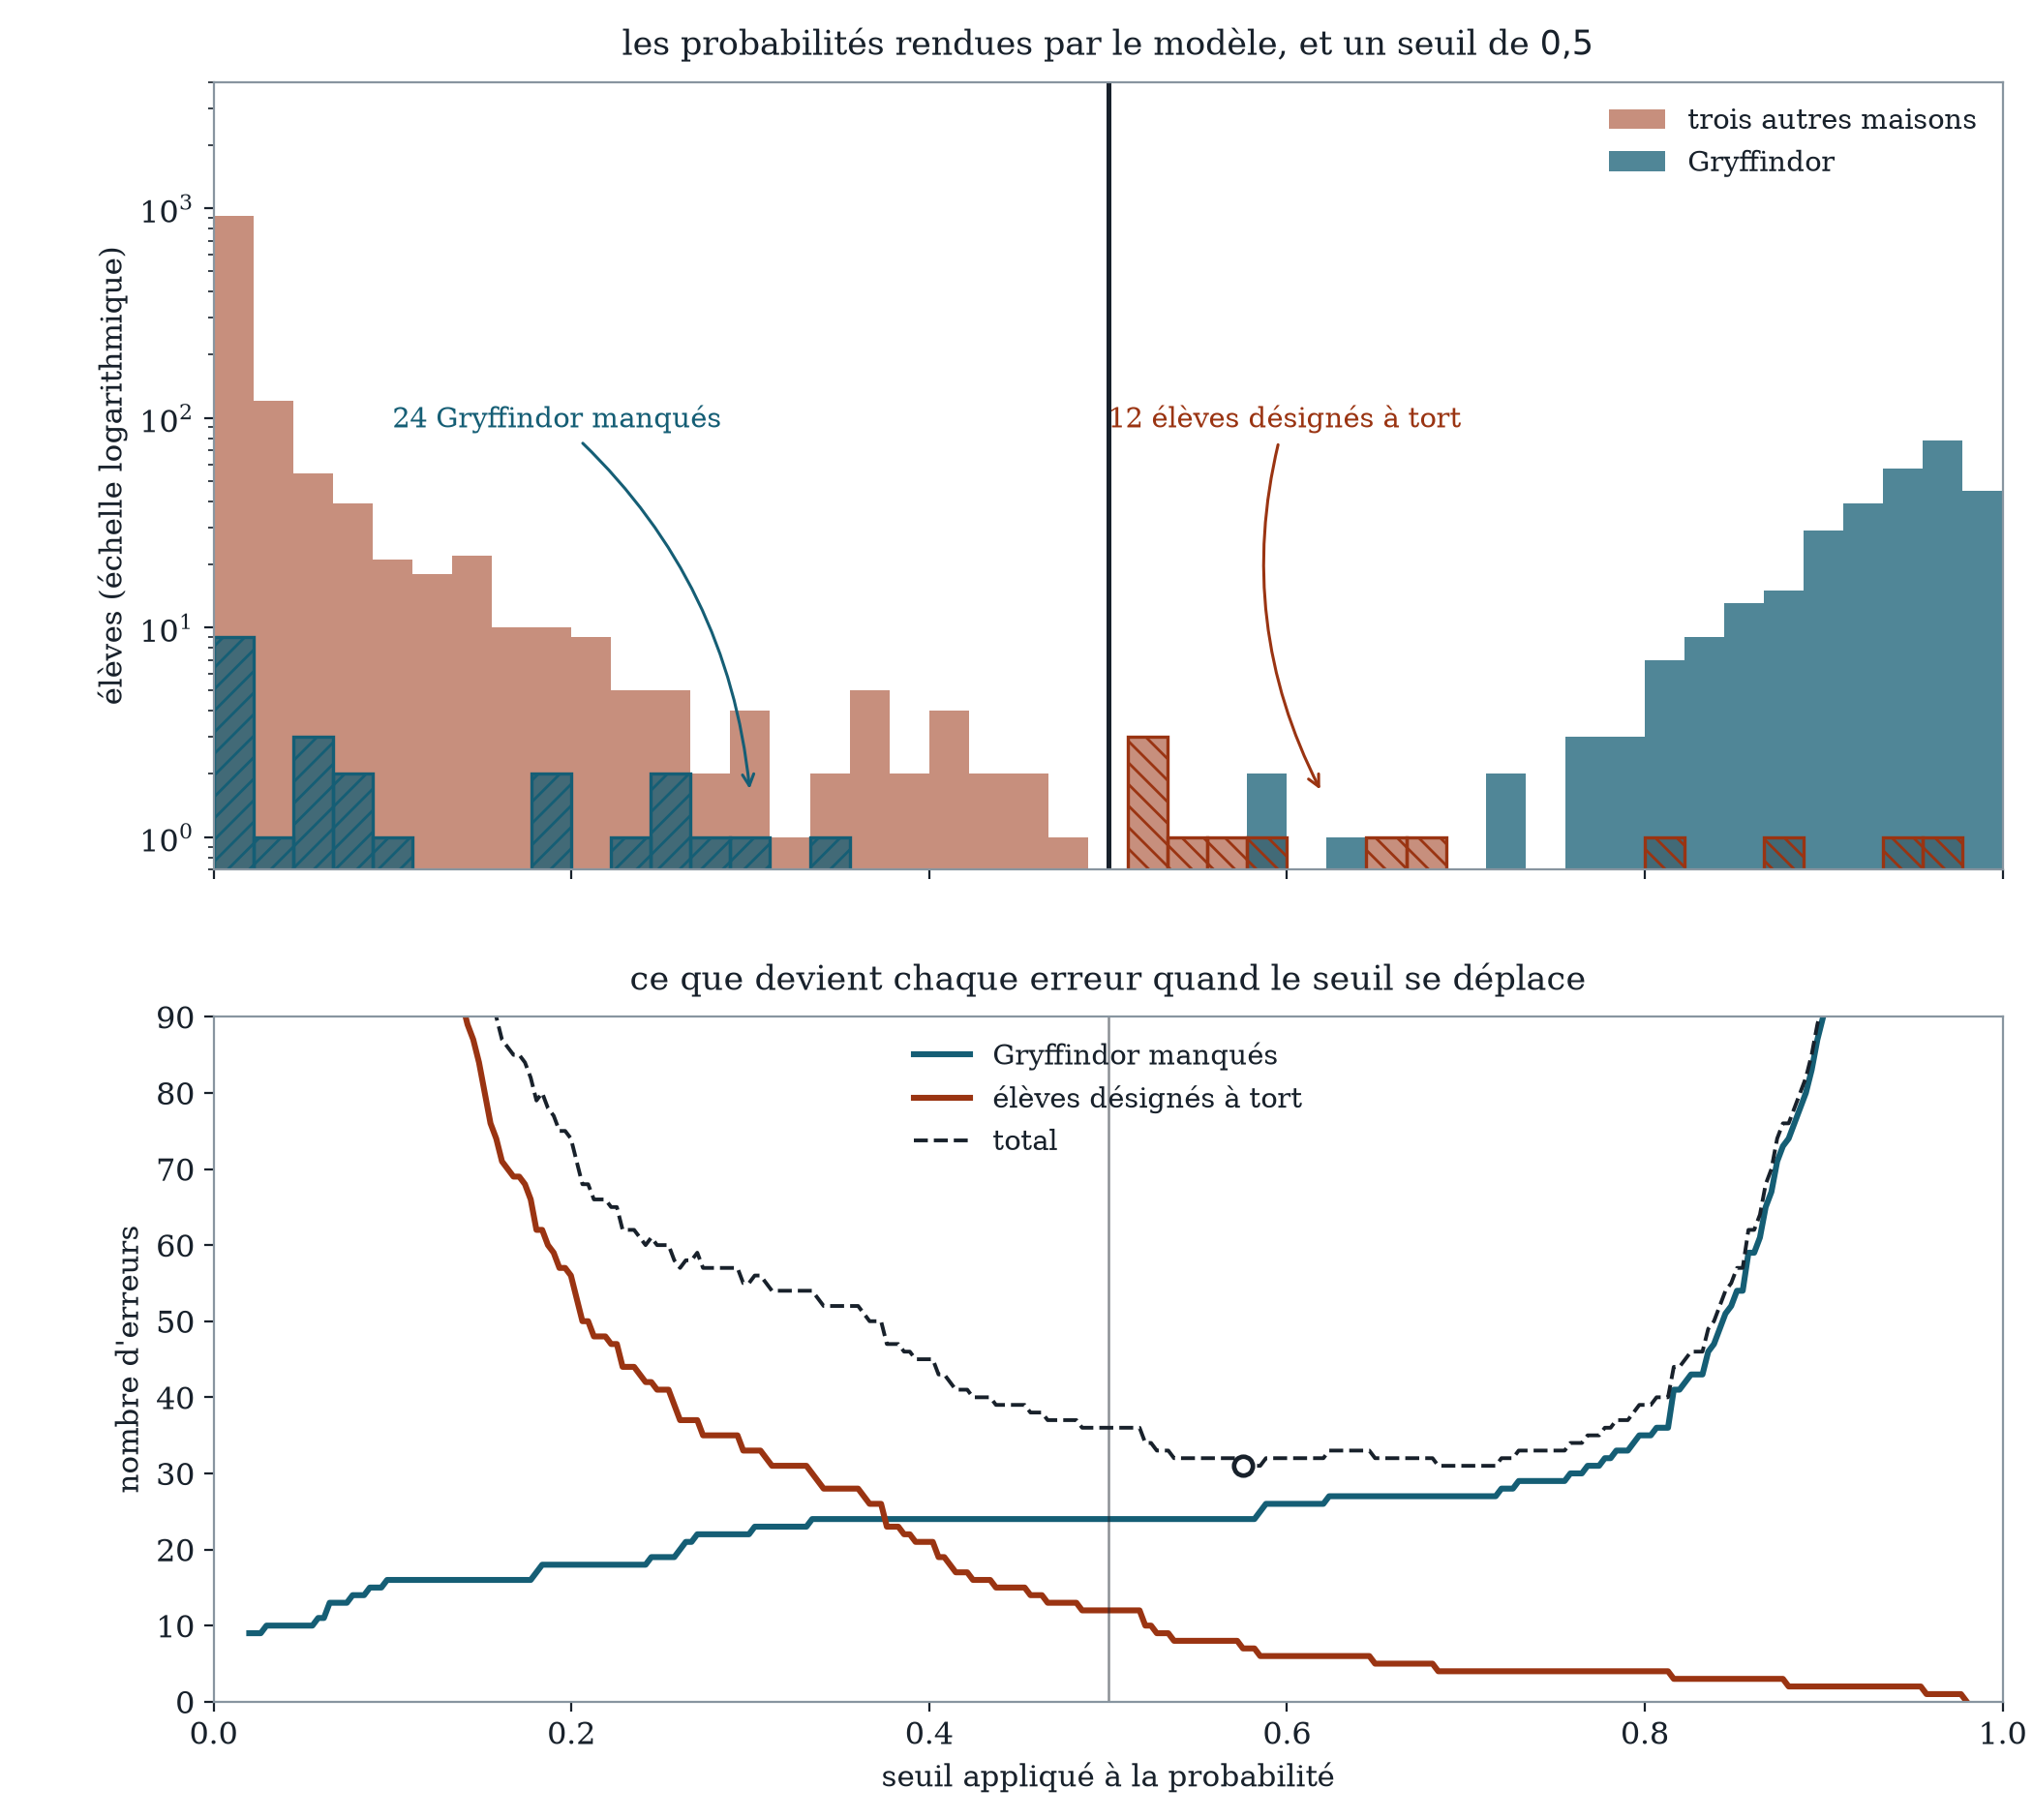
\includegraphics[width=\textwidth,
  alt={Deux panneaux à axe horizontal commun, la probabilité rendue par le modèle. En haut, deux histogrammes en échelle logarithmique séparés selon la classe observée, hachures sur les prédictions incorrectes au seuil 0,5. En bas, deux courbes d'erreurs de sens contraire selon le seuil, et leur somme dont le minimum est cerclé vers 0,58.}]{figures/seuil.png}
\caption{Probabilités par classe observée, en haut ; hachures : erreurs au seuil
$0{,}5$. Nombre d'erreurs selon le seuil, en bas ; minimum cerclé.}
\label{fig:seuil}
\end{figure}
\FloatBarrier

Un seuil $s$ quelconque revient de même à comparer le score au logit de $s$, donc
à tracer la droite $z=\operatorname{logit}(s)$, parallèle à celle de $0{,}5$.
Changer le seuil translate la frontière sans la faire pivoter, ce qui revient à
déplacer le seul biais $w_0$ (ch.~\ref{ch:nuage}).

\begin{figure}[htbp]
\centering
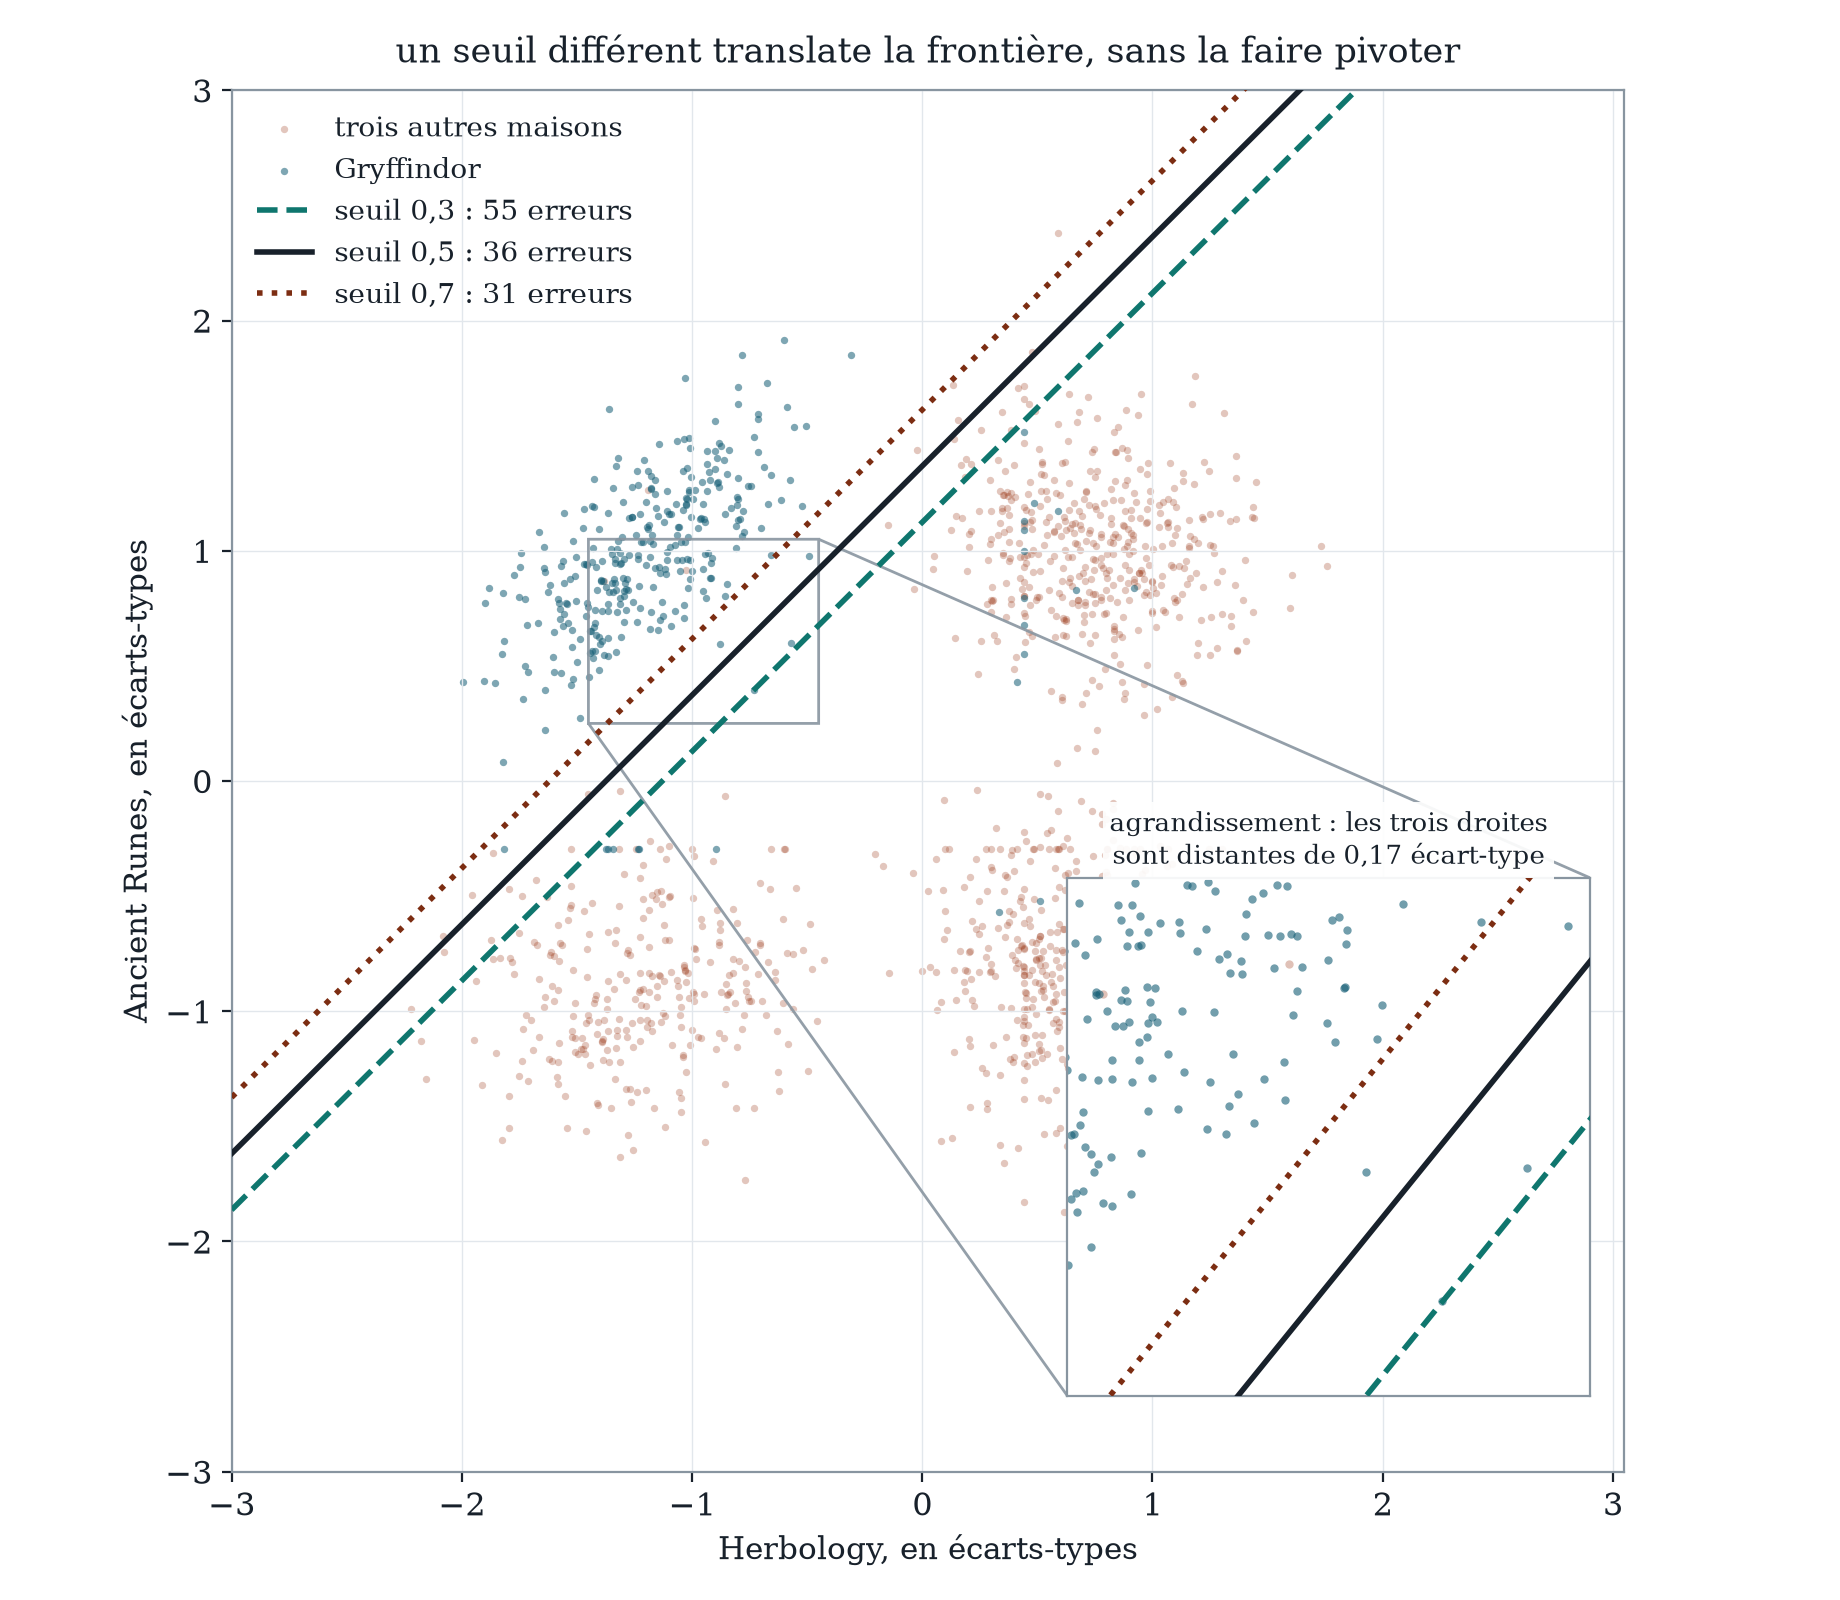
\includegraphics[width=\textwidth,
  alt={Nuage standardisé traversé par trois droites parallèles correspondant aux seuils 0,3, 0,5 et 0,7. Un agrandissement montre la poignée d'observations comprises entre elles, qui changent de réponse d'un seuil à l'autre.}]{figures/seuil_plan.png}
\caption{Nuage standardisé et droites des seuils $0{,}3$, $0{,}5$ et $0{,}7$ :
même direction, biais décalés. L'agrandissement porte les observations qui
changent de réponse d'une droite à l'autre.}
\label{fig:seuil-plan}
\end{figure}
\FloatBarrier

\begin{releve}
Les trois seuils reviennent aux biais $-3{,}898$, $-4{,}745$ et $-5{,}593$, soit
des droites distantes de $0{,}17$ écart-type.
\end{releve}

\begin{chiffres}[Erreurs selon le seuil, état \Mquatre]
\begin{center}
\begin{tabular}{crrrl}
\toprule
seuil & \Gryf manqués & désignés à tort & total & \\
\midrule
$0{,}30$ & $22$ & $33$ & $55$ & \\
$0{,}50$ & $24$ & $12$ & $36$ & seuil retenu \\
$0{,}58$ & $24$ & $7$  & $31$ & \\
$0{,}5824$ & $23$ & $7$ & $30$ & minimum sur ce fichier \\
$0{,}70$ & $27$ & $4$  & $31$ & \\
\bottomrule
\end{tabular}
\end{center}
Le minimum n'apparaît qu'en balayant les seuils au dix-millième ; une grille plus
grossière rend $31$. Un seuil obtenu par balayage sur les données d'ajustement
est une valeur ajustée de plus, qui se déplacerait sur un autre échantillon.
\end{chiffres}

L'origine de ce décalage tient à l'échantillon, non au déséquilibre des classes.
Sous des probabilités conditionnelles correctement estimées et deux erreurs
comptées au même prix, le seuil qui minimise le nombre d'erreurs vaut $0{,}5$
quel que soit le déséquilibre : c'est la règle de décision de Bayes, et les
proportions de classes n'y interviennent pas. Le rapport de $327$ \Gryf à
$1\,273$ autres élèves est d'ailleurs déjà absorbé par le biais $w_0$, qui
s'ajuste sur la fréquence de base (ch.~\ref{ch:descente}).

Le décalage observé a trois causes : calibration imparfaite des probabilités
estimées, spécification affine approchée de la vraie frontière, et taille finie
de l'échantillon --- déplacer le seuil de $0{,}5$ à $0{,}58$ fait basculer une
poignée d'observations, l'ordre de grandeur du bruit d'échantillonnage. Le
programme garde $0{,}5$, issu d'une décision explicite plutôt que d'un ajustement
sur ce fichier.

Un seuil franchement différent se justifie lorsque les deux erreurs coûtent des
prix différents. Recenser toutes les observations d'une classe quitte à en
désigner quelques-unes de trop conduit à abaisser le seuil ; ne désigner que des
cas sûrs conduit à l'élever. Ce choix relève de l'usage fait des prédictions, que
les données seules laissent ouvert.

À quatre classes, la décision compare les quatre scores et retient le plus grand
(ch.~\ref{ch:classifieur}) ; le seuil ne s'applique donc qu'au sous-problème
binaire. La valeur $0{,}5$ garde partout son autre rôle : probabilité rendue par
$\sigma$ en zéro, elle situe la frontière et donne le coût de départ.

\section{Compléments pour un programme livrable}

Trois ajouts séparent ce qui précède d'un programme utilisable sur un fichier
d'élèves inconnus.

\textbf{Enregistrer le modèle.} Les quatre vecteurs, mais aussi les trois
statistiques par matière, la liste ordonnée des matières et celle des maisons. Un
coefficient s'applique à la note qui occupait sa place pendant l'entraînement, et
le plus grand score ne devient une maison que par la liste des libellés. Perdre
l'un de ces ordres donne des scores justes et des réponses fausses, sans aucune
erreur d'exécution.

\textbf{Appliquer les statistiques d'entraînement à la prédiction.} Un élève
inconnu reçoit la médiane, la moyenne et l'écart-type appris sur les élèves
d'entraînement, jamais les siens. Recalculer ces trois nombres sur les nouvelles
données placerait les scores dans une autre échelle ; sur un fichier d'un seul
élève, l'écart-type serait nul et l'opération n'aurait pas de sens.

\textbf{Consigner le protocole.} La graine du découpage, la proportion retenue,
les statistiques ajustées et la date de la mesure. Ces quatre éléments rendent le
chiffre annoncé reproductible, condition pour qu'il constitue un résultat.

\section{Micro-cas de transfert}
\label{sec:transfert}

Le fil rouge a fourni un seul jeu de données. Le micro-cas suivant reprend la
chaîne entière sur douze observations d'un autre domaine, dans d'autres unités,
et fait apparaître un comportement que les $1\,600$ élèves masquaient.

\begin{table}[htbp]
\centering
\small
\setlength{\tabcolsep}{5pt}
\begin{tabular}{rrc rrc rrc}
\toprule
\multicolumn{2}{c}{mesures} & classe &
\multicolumn{2}{c}{mesures} & classe &
\multicolumn{2}{c}{mesures} & classe \\
$d$ & $H$ & & $d$ & $H$ & & $d$ & $H$ & \\
\midrule
$10{,}02$ & $121$ & $0$ & $9{,}96$  & $127$ & $0$ & $10{,}35$ & $147$ & $1$ \\
$10{,}05$ & $118$ & $0$ & $10{,}07$ & $116$ & $0$ & $9{,}71$  & $145$ & $1$ \\
$9{,}98$  & $124$ & $0$ & $10{,}31$ & $143$ & $1$ & $10{,}24$ & $136$ & $1$ \\
$10{,}01$ & $119$ & $0$ & $10{,}28$ & $139$ & $1$ & $9{,}68$  & $141$ & $1$ \\
\bottomrule
\end{tabular}
\caption{Douze pièces usinées : diamètre $d$ en millimètres, dureté $H$ en
vickers, classe $1$ pour un rebut. Les deux colonnes diffèrent d'un facteur
cinquante en échelle.}
\label{tab:micro}
\end{table}

\begin{tache}{Transfert : douze pièces, deux mesures}
\tlab{Contrat} Reprendre \texttt{score\_of}, \texttt{sigmoid},
\texttt{student\_cost}, \texttt{gradient} et la boucle sans les modifier ;
n'écrire que la lecture du tableau et la standardisation des deux colonnes.

\tlab{Contrôle}
\begin{center}\ttfamily\footnotesize
diametre mean 10.0550 sd 0.2071\\
durete\ \ \ mean 131.3333 sd 11.1305\\
cost with zero weights: 0.693147\\[3pt]
stopped after 6000 iterations (plafond), cost 0.000595\\
weights: -0.2721 +1.8591 +11.6553\\
12/12 pieces classees correctement
\end{center}

\tlab{Indice 1} Le coût de départ vaut $\log 2$ ici comme ailleurs : il ne
dépend ni du nombre d'observations, ni de leurs unités.

\tlab{Indice 2} La boucle sort par le plafond, non par la stagnation. Comparer
$\|w\|$ au tour $1\,000$ et au tour $6\,000$ avant de conclure à une erreur de
programmation.

\tlab{Transfert} Les douze pièces sont linéairement séparables. Expliquer
pourquoi la perte tend vers zéro sans que la descente s'arrête, en quoi le
plafond d'itérations est ici le seul critère qui puisse trancher, et ce que
deviendrait la frontière avec un plafond dix fois plus grand
(\annexeref{ann:norme}). Prédire ensuite la classe d'une pièce mesurant
$10{,}20$~mm pour $133$~HV, puis vérifier : $x=(+0{,}700\,;+0{,}150)$ et
$z=+2{,}775$.
\corrige{transfert\_micro.py}
\end{tache}


\appendix
\part{Fondements, démonstrations et compléments}
% !TeX root = ../regression_logistique.tex
\chapter{Notation et vocabulaire}
\label{ann:notation}

\orient{%
retrouver la définition, la dimension et le lieu d'introduction d'un symbole ;
passer du vocabulaire français au vocabulaire anglais de référence}{%
aucun}{%
référence ponctuelle ; revenir au chapitre indiqué dans la dernière colonne}

\section{Indices et dimensions}

\begin{table}[htbp]
\centering
\begin{tabular}{c>{\raggedright\arraybackslash}p{74mm}c}
\toprule
symbole & désignation & introduit \\
\midrule
$m$ & nombre d'observations d'un ensemble ; $1\,600$ pour le fichier entier
  & repère~\ref{ch:probleme} \\
$n$ & nombre de variables explicatives ; $2$ en partie~I, $10$ pour le modèle
    complet & ch.~\ref{ch:nuage} \\
$i$ & indice d'observation, de $1$ à $m$ & ch.~\ref{ch:erreur} \\
$j,k$ & indices de coefficient, de $0$ à $n$ ; l'indice $0$ est celui du biais
  & ch.~\ref{ch:descente} \\
$K$ & nombre de classes ; $4$ ici & ch.~\ref{ch:classifieur} \\
\bottomrule
\end{tabular}
\caption{La somme sur les coefficients commence à $j=0$ parce que le biais est
traité comme un coefficient ordinaire, associé à une colonne de $1$.}
\label{tab:not-indices}
\end{table}

\section{Données}

\begin{table}[htbp]
\centering
\begin{tabular}{c>{\raggedright\arraybackslash}p{74mm}c}
\toprule
symbole & désignation & introduit \\
\midrule
$v$ & note brute, telle qu'elle figure dans le fichier
  & ch.~\ref{ch:standardisation} \\
$\mu$ & moyenne d'une colonne, mesurée sur l'apprentissage
  & ch.~\ref{ch:standardisation} \\
$\sigma$ & écart-type d'une colonne, mesuré sur l'apprentissage
  & ch.~\ref{ch:standardisation} \\
$x_j$ & note standardisée dans la matière $j$, soit $(v-\mu)/\sigma$
  & ch.~\ref{ch:standardisation} \\
$x_0$ & colonne constante égale à $1$, porteuse du biais
  & ch.~\ref{ch:donnees} \\
$\x$ & vecteur $(x_0,x_1,\dots,x_n)$ d'une observation & ch.~\ref{ch:nuage} \\
$x_{ij}$ & note standardisée de l'observation $i$ dans la matière $j$
  & ch.~\ref{ch:descente} \\
$\X$ & tableau des $m$ vecteurs d'observation & ch.~\ref{ch:classifieur} \\
$y_i$ & étiquette de référence de l'observation $i$ : $1$ pour la classe
  traitée, $0$ sinon & ch.~\ref{ch:nuage} \\
\bottomrule
\end{tabular}
\caption{La cote standard $(v-\mu)/\sigma$ est notée $x$ et non $z$, contrairement
à l'usage statistique, la lettre $z$ étant réservée au score du modèle.}
\label{tab:not-donnees}
\end{table}

\section{Paramètres et modèle}

\begin{table}[htbp]
\centering
\begin{tabular}{c>{\raggedright\arraybackslash}p{74mm}c}
\toprule
symbole & désignation & introduit \\
\midrule
$w_0$ & biais, coefficient de la colonne constante & ch.~\ref{ch:nuage} \\
$w_j$ & coefficient de la matière $j$ & ch.~\ref{ch:nuage} \\
$\w$ & vecteur $(w_0,w_1,\dots,w_n)$ de tous les coefficients
  & ch.~\ref{ch:erreur} \\
$w$ & vecteur normal $(w_1,\dots,w_n)$, \emph{biais exclu}, employé dans les
  passages géométriques & ch.~\ref{ch:nuage} \\
$\|w\|$ & norme du seul vecteur normal ; vaut $4{,}89$ pour \Mquatre
  & ch.~\ref{ch:nuage} \\
$\|\w\|$ & norme de tous les coefficients ; vaut $6{,}82$ pour \Mquatre
  & \annexeref{ann:norme} \\
$\alpha$ & taux d'apprentissage & ch.~\ref{ch:descente} \\
$\varepsilon$ & seuil de stagnation du critère d'arrêt & ch.~\ref{ch:entrainer} \\
$s$ & seuil de décision sur la probabilité ; $0{,}5$ ici
  & ch.~\ref{ch:probabilite} \\
$\mu$ (régularisation) & coefficient du terme $\tfrac{\mu}{2}\|\w\|^2$
  & \annexeref{ann:norme} \\
\bottomrule
\end{tabular}
\caption{Deux normes distinctes. $\|w\|$, sans le biais, fixe la raideur de la sigmoïde
le long de la perpendiculaire à la frontière ; $\|\w\|$, biais compris, sert à
la régularisation et à la divergence.}
\label{tab:not-parametres}
\end{table}

\section{Fonctions et quantités calculées}

\begin{table}[htbp]
\centering
\begin{tabular}{c>{\raggedright\arraybackslash}p{74mm}c}
\toprule
symbole & désignation & introduit \\
\midrule
$z$ & score, $\sum_j w_jx_j$ & ch.~\ref{ch:nuage} \\
$\sigma(z)$ & fonction logistique, $1/(1+e^{-z})$ & ch.~\ref{ch:probabilite} \\
$p$ & probabilité annoncée pour la classe traitée, $p=\sigma(z)$
  & ch.~\ref{ch:probabilite} \\
$\ell$ & perte associée à une prédiction & ch.~\ref{ch:erreur} \\
$J(\w)$ & perte moyenne sur un ensemble d'observations & ch.~\ref{ch:erreur} \\
$L(\w)$ & vraisemblance & \annexeref{ann:cout} \\
$\nabla J$ & gradient de $J$, vecteur des $n+1$ dérivées partielles
  & ch.~\ref{ch:descente} \\
$\operatorname{softplus}(z)$ & $\log(1+e^{z})$ & \annexeref{ann:stabilite} \\
$\operatorname{logit}(p)$ & $\log\bigl(p/(1-p)\bigr)$ & ch.~\ref{ch:nuage} \\
$d$ & distance signée d'une observation à la frontière, $z/\|w\|$
  & ch.~\ref{ch:nuage} \\
$s_i$ & $\sigma(z_i)(1-\sigma(z_i))$, facteur de la hessienne
  & \annexeref{ann:convexite} \\
\bottomrule
\end{tabular}
\caption{La lettre $\sigma$ désigne l'écart-type d'une colonne dans les passages
sur la préparation des données, et la fonction logistique partout ailleurs. La
distinction se lit à l'argument : $\sigma$ seul est un écart-type, $\sigma(z)$
est une fonction.}
\label{tab:not-fonctions}
\end{table}

\section{États du modèle}

Le tableau~\ref{tab:etats} du repère~\ref{ch:contrat} nomme les quatre jeux de
coefficients employés : \Mzero, \Mquatre, \Mstop et \Movr. Toute valeur
numérique citée dans le document se rapporte à l'un d'eux, et le nom est rappelé
dans la légende de la figure ou du tableau concerné.

\section{Glossaire}

\begin{table}[htbp]
\centering
\small
\begin{tabular}{>{\raggedright\arraybackslash}p{40mm}>{\raggedright\arraybackslash}p{40mm}>{\raggedright\arraybackslash}p{54mm}}
\toprule
français & anglais & remarque \\
\midrule
cote & odds & rapport $p/(1-p)$, non une probabilité \\
log-cote, logit & log-odds, logit & \\
fonction logistique & logistic function, sigmoid & \\
score & score, logit, linear predictor & « logit » désigne aussi le score dans
  la littérature d'apprentissage \\
entropie croisée binaire & binary cross-entropy & aussi \emph{log-loss} \\
vraisemblance & likelihood & \\
descente de gradient & gradient descent & ici en lot complet, \emph{batch} \\
taux d'apprentissage & learning rate & \\
frontière de décision & decision boundary & \\
vecteur normal & normal vector, weight vector & \\
hyperplan affine & affine hyperplane & \\
un-contre-tous & one-vs-rest, one-vs-all & \cite{rifkin2004} \\
matrice de confusion & confusion matrix & \\
rappel & recall, sensitivity & \\
précision & precision & \\
apprentissage / test & training / test set & \\
fuite de données & data leakage & \\
surapprentissage & overfitting & \\
convexe, strictement convexe & convex, strictly convex & deux propriétés
  distinctes (\annexeref{ann:convexite}) \\
séparabilité linéaire & linear separability & \cite{albert1984} \\
régularisation & regularisation & \\
cote standard & $z$-score, standard score & notée $x$ ici \\
imputation & imputation & \cite{littlerubin2019} \\
\bottomrule
\end{tabular}
\caption{Les sorties console des programmes de la partie~II sont en anglais,
comme les noms de fonctions : c'est la langue des identifiants du projet. Le
texte, lui, emploie systématiquement le terme français.}
\label{tab:glossaire}
\end{table}

% !TeX root = ../regression_logistique.tex
\chapter{Rappels de prérequis}
\label{ann:prerequis}

\orient{%
réactiver les outils de statistique, d'analyse et de géométrie employés par le
cours}{%
aucun}{%
référence ponctuelle ; chaque section indique le chapitre ou l'annexe de retour}

\section{Résumer une colonne de nombres}

Soit $v_1,\dots,v_m$ les valeurs observées dans une colonne.

\textbf{Moyenne.} $\mu=\frac{1}{m}\sum_i v_i$. Elle se déplace avec chaque
valeur : ajouter mille points à la plus haute note déplace $\mu$ de
$1000/m$.

\textbf{Médiane.} La valeur qui coupe la colonne triée en deux moitiés de même
effectif ; pour un effectif pair, la demi-somme des deux valeurs centrales.
Déplacer la plus haute note ne la change pas tant que l'ordre des valeurs
centrales est préservé. C'est cette insensibilité qu'on appelle
\emph{robustesse}.

\textbf{Écart-type.} $\sigma=\sqrt{\frac{1}{m}\sum_i(v_i-\mu)^2}$ : la racine de
la moyenne des carrés des écarts à la moyenne. Il s'exprime dans l'unité de la
colonne et mesure la dispersion typique autour de $\mu$.

\textbf{Cote standard.} $(v-\mu)/\sigma$ exprime un écart en nombre d'écarts-types.
La colonne transformée a pour moyenne $0$ et pour écart-type $1$.

Employés au chapitre~\ref{ch:standardisation}.

\begin{rappel}[Valeur manquante]
Une case vide représente une valeur inconnue. Trois traitements existent :
écarter la ligne,
écarter la colonne, ou attribuer une valeur --- l'\emph{imputation}. Le choix
dépend du mécanisme qui a produit l'absence, question développée
dans~\cite{littlerubin2019} et que ce cours n'aborde pas.
\end{rappel}

\section{Exponentielle, logarithme, cote}

$e^{a}$ est strictement positive, strictement croissante, et transforme les
sommes en produits : $e^{a+b}=e^{a}e^{b}$. Elle parcourt $]0,+\infty[$ quand $a$
parcourt $\R$.

$\log$ est sa réciproque : définie sur $]0,+\infty[$, strictement croissante,
elle parcourt $\R$. Trois égalités servent constamment :
\[
  \log(ab)=\log a+\log b,\qquad
  \log\frac{a}{b}=\log a-\log b,\qquad
  \log a^{b}=b\log a .
\]
Avec $\log 1=0$ et $\log e^{a}=a$.

Le logarithme employé dans tout le document est le logarithme népérien, celui de
base $e$ ; c'est celui que \texttt{math.log} calcule en Python.

\textbf{Cote.} Le rapport $p/(1-p)$ d'une probabilité à son complément. Une
probabilité de $0{,}8$ donne une cote de $4$ : quatre fois plus de chances que
l'événement se produise que le contraire. Quand $p$ parcourt $]0,1[$, la cote
parcourt $]0,+\infty[$ et son logarithme parcourt $\R$.

Employés aux chapitres~\ref{ch:nuage} et~\ref{ch:erreur}, et à
l'\annexeref{ann:logit}.

\section{Vecteurs, produit scalaire, norme}

Dans $\R^n$ muni d'un repère orthonormé, le \emph{produit scalaire} de
$u=(u_1,\dots,u_n)$ et $v=(v_1,\dots,v_n)$ vaut
\[
  u\cdot v=\sum_{j=1}^{n} u_jv_j = \|u\|\,\|v\|\cos\theta,
\]
où $\theta$ est l'angle entre les deux vecteurs et
$\|u\|=\sqrt{\sum_j u_j^2}$ la \emph{norme} de $u$, c'est-à-dire sa longueur.

Trois conséquences employées au chapitre~\ref{ch:nuage} :

\begin{panelitemize}[accent]
  \panelbullet{$u\cdot v=0$ équivaut à $u\perp v$, les deux vecteurs étant non
    nuls ;}
  \panelbullet{$\|v\|\cos\theta$ est la longueur de la projection de $v$ sur la
    direction de $u$, comptée avec un signe ;}
  \panelbullet{multiplier $u$ par $\lambda>0$ multiplie $u\cdot v$ par
    $\lambda$ sans changer le signe ni la direction.}
\end{panelitemize}

\begin{vigilance}[Le repère doit être orthonormé]
Angle, perpendiculaire et distance n'ont le sens usuel que si les deux axes
portent la même unité. Sur les notes brutes, où un axe se gradue en points et
l'autre en centaines de points, ces notions dépendent du barème. La
standardisation du chapitre~\ref{ch:standardisation} fournit un système d'unités
commun ; elle ne rend pas pour autant la géométrie obtenue équivalente à celle
des données brutes, point discuté au même chapitre.
\end{vigilance}

\section{Dérivée, dérivée partielle, gradient}

La \emph{dérivée} $f'(a)$ mesure la variation de $f$ par unité de variation de
son argument, au voisinage de $a$ : c'est la pente de la tangente en ce point.
Son signe indique le sens de variation, sa valeur absolue la rapidité.

Trois règles suffisent aux calculs du document :
\[
  (u+v)'=u'+v',\qquad
  \left(\frac{1}{u}\right)'=-\frac{u'}{u^{2}},\qquad
  \bigl(f\circ g\bigr)'(a)=f'\bigl(g(a)\bigr)\,g'(a) .
\]
La troisième est la \emph{règle de chaîne}, employée dans toute
l'\annexeref{ann:gradient}.

La \emph{dérivée partielle} $\partial J/\partial w_j$ est la dérivée de $J$
considérée comme fonction du seul $w_j$, les autres coefficients étant tenus
pour constants. Le \emph{gradient} $\nabla J$ est le vecteur de ces dérivées
partielles.

Deux propriétés servent au chapitre~\ref{ch:descente} :

\begin{panelitemize}[rulecolor]
  \panelbullet{$-\nabla J$ est la direction de plus forte décroissance locale de
    $J$ au point considéré ;}
  \panelbullet{$\nabla J$ est orthogonal à la ligne de niveau de $J$ passant par
    ce point.}
\end{panelitemize}

\begin{rappel}[Approximation locale]
Pour un déplacement $\delta$ petit,
$J(\w+\delta)\approx J(\w)+\nabla J(\w)\cdot\delta$. Cette approximation est
locale : elle cesse de décrire $J$ dès que $\delta$ sort du voisinage où la
pente mesurée reste représentative. C'est la raison pour laquelle un pas de
descente trop long peut faire monter le coût
(ch.~\ref{ch:descente}).
\end{rappel}

\section{Dérivée seconde et courbure}

La dérivée seconde $f''$ mesure la variation de la pente. Positive sur un
intervalle, elle y rend $f'$ croissante, donc $f'$ y traverse zéro au plus une
fois.

Pour une fonction de plusieurs variables, la \emph{hessienne} est le tableau
carré des dérivées secondes $\partial^2 J/\partial w_j\partial w_k$. La courbure
de $J$ dans une direction $\mathbf v$ vaut $\mathbf v^{\!\top}H\mathbf v$. Ces
notions servent à l'\annexeref{ann:convexite}.

% !TeX root = ../regression_logistique.tex
\chapter{Construction de la fonction logistique}
\label{ann:logit}

\orient{%
construire le logit comme composée de la cote et du logarithme ; inverser
l'hypothèse~\eqref{eq:logit} pour obtenir $\sigma$ ; énoncer ce que cette
construction établit et ce qu'elle suppose}{%
exponentielle, logarithme, cote (\annexeref{ann:prerequis}) ;
chapitre~\ref{ch:nuage}}{%
approfondissement ; le fil principal n'emploie que la formule encadrée}

\section{Première transformation : la cote}

Une probabilité $p$ appartient à $[0,1]$. Le rapport
\[
  \frac{p}{1-p}
\]
s'appelle la \emph{cote}. C'est le langage des paris : une cote de $3$ signifie
trois chances contre une. Ce rapport vaut $0$ quand $p=0$, vaut $1$ quand
$p=0{,}5$, et croît sans borne quand $p$ approche $1$.

\begin{table}[htbp]
\centering
\begin{tabular}{rrrr}
\toprule
$p$ & $1-p$ & cote $p/(1-p)$ & $\log$ de la cote \\
\midrule
$0{,}10$ & $0{,}90$ & $0{,}111$ & $-2{,}197$ \\
$0{,}25$ & $0{,}75$ & $0{,}333$ & $-1{,}099$ \\
$0{,}50$ & $0{,}50$ & $1{,}000$ & $0{,}000$ \\
$0{,}75$ & $0{,}25$ & $3{,}000$ & $+1{,}099$ \\
$0{,}90$ & $0{,}10$ & $9{,}000$ & $+2{,}197$ \\
\bottomrule
\end{tabular}
\caption{La cote transporte $[0,1]$ vers $[0,+\infty[$, son logarithme vers
$\R$ tout entier. La dernière colonne est symétrique autour de $p=0{,}5$ : c'est
la propriété que le score doit posséder.}
\label{tab:cotes}
\end{table}

La cote atteint ainsi toutes les valeurs positives ; restent les négatives.

\begin{figure}[htbp]
\centering
\begin{graphique}{Trois axes superposés reliés par des flèches. Le premier porte l'intervalle de 0 à 1 avec 0,5 au milieu. Le deuxième, le demi-axe des cotes de 0 à l'infini avec 1 au repère. Le troisième, la droite réelle entière avec 0 au repère.}
\begin{tikzpicture}[font=\small,
  seg/.style={line width=1.4pt},
  bnd/.style={font=\scriptsize,text=ink!75},
  op/.style={font=\footnotesize,text=accent,align=center},
  arr/.style={-{Latex[length=2.2mm]},thick,ink!55}]

\draw[seg,gryff!70] (0,0) -- (4.4,0);
\node[bnd,anchor=north] at (0,-0.18) {$0$};
\node[bnd,anchor=north] at (4.4,-0.18) {$1$};
\node[font=\footnotesize,text=ink,anchor=south] at (2.2,0.18) {$p$};

\draw[seg,huffle!70] (0,-2) -- (4.4,-2);
\draw[huffle!70,line width=1.4pt,dashed] (4.4,-2) -- (5.1,-2);
\node[bnd,anchor=north] at (0,-2.18) {$0$};
\node[bnd,anchor=north] at (2.05,-2.18) {$1$};
\node[bnd,anchor=north] at (5.2,-2.18) {$+\infty$};
\fill[huffle!70] (2.05,-2.12) rectangle (2.09,-1.88);
\node[font=\footnotesize,text=ink,anchor=south] at (2.2,-1.82)
  {$\dfrac{p}{1-p}$};

\draw[seg,raven!70] (-1.3,-4) -- (5.1,-4);
\draw[raven!70,line width=1.4pt,dashed] (-2,-4) -- (-1.3,-4);
\node[bnd,anchor=north] at (-2.1,-4.18) {$-\infty$};
\node[bnd,anchor=north] at (2.05,-4.18) {$0$};
\node[bnd,anchor=north] at (5.2,-4.18) {$+\infty$};
\fill[raven!70] (2.05,-4.12) rectangle (2.09,-3.88);
\node[font=\footnotesize,text=ink,anchor=south] at (2.2,-3.82)
  {$\log\dfrac{p}{1-p}$};

\draw[arr] (6.4,0) -- (6.4,-1.6);
\node[op,anchor=west] at (6.6,-0.8) {rapport à\\ son complément};
\draw[arr] (6.4,-2.4) -- (6.4,-3.6);
\node[op,anchor=west] at (6.6,-3.0) {logarithme};
\end{tikzpicture}
\end{graphique}
\caption{Les trois intervalles. La cote étire $]0,1[$ sur $]0,+\infty[$ en envoyant
$0{,}5$ sur $1$ ; le logarithme envoie ce demi-axe sur $\R$. La composée est une
bijection croissante de $]0,1[$ sur $\R$, l'une des infinités qui rendent
l'égalité avec le score possible (section~2).}
\label{fig:intervalles}
\end{figure}
\FloatBarrier

\section{Seconde transformation : le logarithme}

Le logarithme envoie $]0,+\infty[$ sur $\R$ : il vaut $-\infty$ près de zéro,
$0$ en $1$, et croît sans borne. En le composant avec la cote, on obtient la
\emph{log-cote}
\[
  \log\frac{p}{1-p},
\]
qui prend toutes les valeurs réelles, comme le score $z$. Les deux quantités
parcourant le même ensemble, poser leur égalité est \emph{possible} :
% \tag ne fait pas avancer le compteur : sans ce pas, l'ancre PDF de cette
% équation entre en collision avec celle de la première équation numérotée.
\begin{equation}
  \boxed{\;\log\frac{p}{1-p}=z=\sum_{j=0}^{n}w_jx_j\;}
  \tag{$\star$}\label{eq:logit}
\end{equation}
\stepcounter{equation}

L'égalité~\eqref{eq:logit} constitue un choix parmi les bijections croissantes
de $]0,1[$ sur $\R$. La réciproque de la fonction de
répartition de la loi normale donne le modèle \emph{probit}, celle de la loi de
Gumbel le modèle \emph{complémentaire log-log} (ch.~\ref{ch:nuage}). Le logit est
donc une hypothèse de modélisation, retenue pour trois raisons : il donne aux
coefficients une lecture directe en log-cotes, il est le lien canonique du modèle
linéaire généralisé binomial, ce qui produit les formules les plus
simples~\cite{mccullagh1989}, et il conduit à une perte convexe
(\annexeref{ann:convexite}). Le modèle en compte deux autres, posées ailleurs :
l'indépendance conditionnelle des observations (\annexeref{ann:cout}) et le choix
des variables retenues.

Les annexes suivantes tirent les conséquences de~\eqref{eq:logit} : l'expression
de $p$ en fonction de $z$ ci-dessous, les propriétés de $\sigma$
(\annexeref{ann:sigmoide}), la perte (\annexeref{ann:cout}) et le gradient
(\annexeref{ann:gradient}).

\section{Expression de \texorpdfstring{$p$}{p} en fonction de \texorpdfstring{$z$}{z}}

L'équation~\eqref{eq:logit} donne $z$ à partir de $p$, alors que le programme
part de $z$ pour obtenir la probabilité. L'inversion consiste à isoler $p$ ;
chaque ligne porte à droite l'opération qui la produit.

\begin{align}
  \log\frac{p}{1-p} &= z \notag\\[2pt]
  e^{\log\frac{p}{1-p}} &= e^{z}
    &&\text{on applique } e^{\;\cdot\;} \text{ aux deux membres} \notag\\[2pt]
  \frac{p}{1-p} &= e^{z}
    &&\text{car } e^{\log a}=a \notag\\[2pt]
\end{align}

\slidebreak

\begin{align}
  p &= e^{z}(1-p)
    &&\text{on multiplie les deux membres par } 1-p \notag\\[2pt]
  p &= e^{z}-e^{z}p
    &&\text{on développe} \notag\\[2pt]
  p+e^{z}p &= e^{z}
    &&\text{on rassemble les } p \notag\\[2pt]
  p\,(1+e^{z}) &= e^{z}
    &&\text{on met } p \text{ en facteur} \notag\\[2pt]
  p &= \frac{e^{z}}{1+e^{z}}
    &&\text{on divise par } 1+e^{z},\ \text{qui n'est jamais nul} \label{eq:sigma-brute}
\end{align}

Cette écriture se met sous une forme plus courante en divisant numérateur et
dénominateur par $e^{z}$ :
\begin{align}
  p &= \frac{e^{z}}{1+e^{z}}
     = \frac{e^{z}/e^{z}}{(1+e^{z})/e^{z}}
    &&\text{on divise en haut et en bas par } e^{z}\neq0 \notag\\[2pt]
    &= \frac{1}{1/e^{z}+1}
    &&\text{car } e^{z}/e^{z}=1 \notag\\[2pt]
    &= \frac{1}{1+e^{-z}}
    &&\text{car } 1/e^{z}=e^{-z} \label{eq:sigma}
\end{align}

\begin{resultat}[Fonction logistique]
\[
  \sigma(z)=\frac{1}{1+e^{-z}}=\frac{e^{z}}{1+e^{z}} .
\]
Les deux écritures désignent la même fonction, obtenue en inversant
l'hypothèse~\eqref{eq:logit}.
\end{resultat}

Chacune des deux formes échoue là où l'autre tient. Pour $z$ très négatif,
$e^{-z}$ devient
gigantesque et $1/(1+e^{-z})$ déborde la capacité de la machine, tandis que
$e^{z}/(1+e^{z})$ rend $0$. Pour $z$ très positif, c'est
l'inverse. Le programme utilise donc l'une ou l'autre selon le signe de $z$
(\annexeref{ann:stabilite}).

\section{Vérification numérique}

La table~\ref{tab:cotes} se relit dans l'autre sens. Pour $z=1{,}099$ :
\[
  e^{-1{,}099}=0{,}3333,\qquad
  \sigma(1{,}099)=\frac{1}{1+0{,}3333}=\frac{1}{1{,}3333}=0{,}75 .
\]
On retrouve la ligne $p=0{,}75$, dont la log-cote valait $+1{,}099$. Pour
$z=0$ :
\[
  \sigma(0)=\frac{1}{1+e^{0}}=\frac{1}{1+1}=0{,}5 .
\]
Un élève situé exactement sur la droite reçoit une probabilité de $0{,}5$ : la
frontière (ch.~\ref{ch:nuage}) est la ligne de niveau $0{,}5$ du modèle.

\begin{figure}[htbp]
\centering
\begin{graphique}{Courbe de la fonction logistique, en S, croissante de 0 vers 1, valant 0,5 à l'origine, avec ses deux asymptotes horizontales en pointillé.}
\begin{tikzpicture}
\begin{axis}[courseplot,height=6.4cm,axis lines=middle,
  xlabel={score $z$},ylabel={$\sigma(z)$},
  xmin=-6.5,xmax=6.5,ymin=-.12,ymax=1.15,ytick={0,.25,.5,.75,1},
  samples=200,domain=-6.5:6.5]
  \addplot[gridgray,thick,dashed,domain=-6.5:6.5]{1};
  \addplot[accent,very thick]{1/(1+exp(-x))};
  \addplot[only marks,mark=*,warning,mark size=2.6pt]
    coordinates {(0,0.5) (1.099,0.75) (-1.099,0.25)};
  \node[warning,anchor=west,font=\small] at (axis cs:1.3,.78){$(1{,}099\,;\,0{,}75)$};
  \node[warning,anchor=east,font=\small] at (axis cs:-1.3,.22){$(-1{,}099\,;\,0{,}25)$};
  \node[ink,anchor=south west,font=\small] at (axis cs:.15,.5){$\sigma(0)=0{,}5$};
\end{axis}
\end{tikzpicture}
\end{graphique}
\caption{La fonction logistique envoie $\R$ dans l'intervalle $]0,1[$, sans
jamais atteindre les bornes, et passe par $0{,}5$ à l'origine.}
\label{fig:sigmoide}
\end{figure}
\FloatBarrier

\begin{vigilance}[Valeurs prises par $\sigma$]
Pour $z$ fini, $1+e^{-z}$ reste strictement plus grand que $1$, donc $\sigma(z)$
reste strictement compris entre $0$ et $1$. Toute probabilité produite par le
modèle appartient donc à l'intervalle ouvert $]0,1[$. En machine, $\sigma(40)$
vaut pourtant exactement $1$ après arrondi : l'écart disparaît à partir d'un
score d'environ $37$, avec les conséquences que cela entraîne dans un logarithme
(\annexeref{ann:stabilite}).
\end{vigilance}

% !TeX root = ../regression_logistique.tex
\chapter{Propriétés de la fonction logistique}
\label{ann:sigmoide}

\orient{%
établir $\sigma(-z)=1-\sigma(z)$ et $\sigma'=\sigma(1-\sigma)$ ; distinguer le
rôle de $\sigma'$ dans la sensibilité de la probabilité et dans le gradient}{%
règle de chaîne, dérivée d'un inverse (\annexeref{ann:prerequis})}{%
approfondissement ; le fil principal n'emploie que les deux égalités encadrées}

\section{Symétrie}

Échanger les deux réponses revient à changer le signe du score, la frontière
étant le lieu où il s'annule. La fonction logistique doit donc échanger $p$ et
$1-p$ lorsqu'on passe de $z$ à $-z$, ce que le calcul confirme.

\begin{align}
  \sigma(-z) &= \frac{1}{1+e^{-(-z)}}
    &&\text{définition, avec } -z \text{ à la place de } z \notag\\[2pt]
  &= \frac{1}{1+e^{z}}
    &&\text{car } -(-z)=z \notag\\[2pt]
\end{align}

\slidebreak

Et par ailleurs :
\begin{align}
  1-\sigma(z) &= 1-\frac{1}{1+e^{-z}}
    &&\text{définition} \notag\\[2pt]
  &= \frac{(1+e^{-z})-1}{1+e^{-z}}
    &&\text{même dénominateur} \notag\\[2pt]
  &= \frac{e^{-z}}{1+e^{-z}}
    &&\text{on simplifie le numérateur} \notag
\end{align}

\slidebreak

\begin{align}
  1-\sigma(z)
  &= \frac{e^{-z}}{1+e^{-z}}\cdot\frac{e^{z}}{e^{z}}
    &&\text{on multiplie par } 1 \text{ écrit } e^{z}/e^{z} \notag\\[2pt]
  &= \frac{e^{-z}e^{z}}{e^{z}+e^{-z}e^{z}}
    &&\text{on distribue} \notag\\[2pt]
  &= \frac{1}{e^{z}+1}
    &&\text{car } e^{-z}e^{z}=e^{0}=1 \label{eq:sym}
\end{align}

Les deux résultats coïncident, donc
\[
  \boxed{\;\sigma(-z)=1-\sigma(z)\;}
\]

La probabilité accordée à « \Gryf » pour un score $z$ égale donc celle
accordée à « pas \Gryf » pour le score $-z$.

\begin{releve}
$\sigma(2)=0{,}8808$ et $\sigma(-2)=0{,}1192$, de somme $1$.
\end{releve}

\section{Dérivée}

Écrite $\sigma=1/u$ avec $u=1+e^{-z}$, la fonction se dérive par la règle de
l'inverse, la chaîne fournissant $u'$. Le résultat s'exprime avec $\sigma$
elle-même, ce qui évite d'avoir à réévaluer une exponentielle dans le calcul du
gradient.

\begin{align}
  \sigma(z) &= \frac{1}{1+e^{-z}} = \frac{1}{u},\qquad u=1+e^{-z} \notag\\[4pt]
  u' &= \bigl(1+e^{-z}\bigr)'
     = 0+e^{-z}\cdot(-1)
    &&\text{dérivée d'une somme, puis chaîne sur } e^{-z} \notag\\[2pt]
     &= -e^{-z} \notag\\[6pt]
\end{align}

\slidebreak

\begin{align}
  \sigma'(z) &= -\frac{u'}{u^{2}}
    &&\text{dérivée d'un inverse : } (1/u)'=-u'/u^{2} \notag\\[2pt]
  &= -\frac{-e^{-z}}{(1+e^{-z})^{2}}
    &&\text{on remplace } u \text{ et } u' \notag\\[2pt]
  &= \frac{e^{-z}}{(1+e^{-z})^{2}}
    &&\text{les deux signes moins s'annulent} \notag\\[2pt]
  &= \frac{1}{1+e^{-z}}\cdot\frac{e^{-z}}{1+e^{-z}}
    &&\text{on sépare le carré en deux facteurs} \notag\\[2pt]
  &= \sigma(z)\cdot\bigl(1-\sigma(z)\bigr)
    &&\text{le second facteur est } 1-\sigma(z),\ \text{établi en \eqref{eq:sym}}
\end{align}

\begin{resultat}[Dérivée de la sigmoïde]
\[
  \sigma'(z)=\sigma(z)\bigl(1-\sigma(z)\bigr).
\]
La pente se calcule donc sans nouvelle exponentielle : si l'on connaît déjà
$p=\sigma(z)$, la pente vaut $p(1-p)$.
\end{resultat}

\section{Variation de la probabilité avec le score}

La quantité $p(1-p)$ atteint son maximum, $0{,}25$, en $p=0{,}5$, et décroît vers
$0$ aux deux extrémités : la probabilité varie fortement avec le score près de la
frontière, et très peu lorsqu'elle est déjà proche de $0$ ou de $1$.

\begin{figure}[htbp]
\centering
\begin{graphique}{Deux courbes superposées : la fonction logistique croissante en S, et sa dérivée en cloche symétrique, maximale à 0,25 à l'origine et tendant vers zéro des deux côtés.}
\begin{tikzpicture}
\begin{axis}[courseplot,height=6cm,axis lines=middle,
  xlabel={score $z$},ylabel={},xmin=-6.5,xmax=6.5,ymin=-.08,ymax=1.1,
  samples=200,domain=-6.5:6.5,
  legend style={at={(.5,1.03)},anchor=south,legend columns=2,draw=none}]
  \addplot[accent,very thick]{1/(1+exp(-x))};
  \addlegendentry{$\sigma(z)$}
  \addplot[warning,very thick]{exp(-x)/(1+exp(-x))^2};
  \addlegendentry{$\sigma'(z)=\sigma(z)(1-\sigma(z))$}
  \addplot[only marks,mark=*,ink,mark size=2.4pt] coordinates {(0,0.25)};
  \node[ink,anchor=south west,font=\small] at (axis cs:.2,.25){$0{,}25$};
\end{axis}
\end{tikzpicture}
\end{graphique}
\caption{La dérivée atteint son maximum, $0{,}25$, en $z=0$, et tend vers zéro dès
que la probabilité approche $0$ ou $1$.}
\label{fig:derivee-sigmoide}
\end{figure}
\FloatBarrier

Cette cloche gouverne deux quantités. La première est la sensibilité de la
\emph{probabilité} au score : $p$ varie fortement avec $z$ près de la frontière
et très peu une fois proche de $0$ ou de $1$, ce qui explique qu'agrandir la
norme des coefficients modifie les probabilités sans déplacer la frontière
(\annexeref{ann:norme}). La seconde est la \emph{courbure} de la perte, dont
$\sigma'$ fournit le facteur $s_i$ de la hessienne
(\annexeref{ann:convexite}).

Le poids d'une observation dans le gradient est en revanche
$\partial\ell/\partial z=p-y$ (\annexeref{ann:gradient}) : le facteur
$\sigma(1-\sigma)$ apparaît dans la dérivation, puis se simplifie avec les
dénominateurs venus du logarithme. Les deux quantités se séparent nettement. Sur
la frontière, $p=0{,}5$ : $\sigma'$ atteint son maximum $\frac14$ tandis que
$|p-y|$ vaut $0{,}5$ ; pour une observation d'étiquette $y=1$ classée à
$p=0{,}02$, $\sigma'$ tombe à $0{,}0196$ tandis que $|p-y|$ monte à $0{,}98$. La
correction est donc portée par les prédictions incorrectes et assurées.

% !TeX root = ../regression_logistique.tex
\chapter{Construction du coût par vraisemblance}
\label{ann:cout}

\orient{%
écrire la vraisemblance d'un jeu d'étiquettes sous le modèle ; la transformer en
somme par le logarithme ; en déduire la perte employée par le fil principal ;
nommer les hypothèses qui interviennent}{%
logarithme, exposants (\annexeref{ann:prerequis}) ; chapitre~\ref{ch:erreur}}{%
approfondissement ; le fil principal n'emploie que la formule encadrée}

\section{Probabilité d'une réponse observée}

Notons $y_i$ l'étiquette : $1$ si l'observation $i$ appartient à \Gryf, $0$ sinon, et
$p_i=\sigma(z_i)$ la probabilité produite par le modèle. La probabilité que celui-ci
attribue à l'étiquette effectivement observée vaut $p_i$ si $y_i=1$, et $1-p_i$
si $y_i=0$. Ces deux cas se rassemblent :
\[
  \Pp(y_i)=p_i^{\,y_i}\,(1-p_i)^{\,1-y_i}.
\]

Vérification des deux cas, en se souvenant que $a^{0}=1$ et $a^{1}=a$ :
\[
  y_i=1:\quad p_i^{1}(1-p_i)^{0}=p_i\cdot1=p_i,
  \qquad
  y_i=0:\quad p_i^{0}(1-p_i)^{1}=1\cdot(1-p_i)=1-p_i .
\]
L'exposant nul ramène à $1$ le facteur qui ne correspond pas au cas observé.

\section{Vraisemblance du fichier}

Une seconde hypothèse intervient ici, distincte de celle du lien logit : les
étiquettes sont supposées conditionnellement indépendantes, une fois les notes
connues. C'est elle qui autorise à écrire la probabilité d'observer l'ensemble
des étiquettes du fichier comme le produit des probabilités individuelles :
\[
  L(\w)=\prod_{i=1}^{m}p_i^{\,y_i}(1-p_i)^{\,1-y_i}.
\]
$L$ s'appelle la \emph{vraisemblance}. Elle dépend des coefficients $\w$, car ce
sont eux qui produisent les $p_i$. Chercher les meilleurs coefficients, c'est
chercher ceux qui rendent $L$ maximale.

\begin{vigilance}[Sous-dépassement du produit]
Le produit compte $1\,600$ facteurs, tous strictement inférieurs à $1$, et
décroît donc très vite. Le plus petit double normal vaut environ
$2{,}2\times10^{-308}$ ; en dessous, la précision se dégrade puis le nombre
s'arrondit à zéro~\cite{goldberg1991}.

Le seuil se franchit facilement. Si chaque facteur valait $0{,}5$ --- un modèle
sans opinion --- le produit vaudrait $0{,}5^{1600}\approx10^{-482}$, qui
s'arrondit à zéro. Si chacun valait $0{,}9$, le produit vaudrait
$6{,}1\times10^{-74}$ : représentable, mais déjà privé de toute marge, et un
fichier dix fois plus long le ferait sous-dépasser. Une fois deux vraisemblances
arrondies à zéro, aucune comparaison n'est plus possible.

Le logarithme supprime le problème en transformant le produit en somme, dont
l'ordre de grandeur reste celui du nombre d'observations.
\end{vigilance}

\begin{figure}[htbp]
\centering
\begin{graphique}{Chaîne de trois expressions reliées par des flèches : le produit des probabilités individuelles, puis sa transformation en somme par le logarithme, puis le passage à une moyenne changée de signe, quantité que le programme minimise.}
\begin{tikzpicture}[
  bx/.style={draw=ink!30,rounded corners=2.5pt,align=center,font=\footnotesize,
    inner sep=5pt,text width=26mm,minimum height=13mm},
  op/.style={font=\scriptsize,text=accent,align=center},
  arr/.style={-{Latex[length=2.2mm]},thick,ink!60}]
\node[bx,fill=accentlight] (p) {$m$ probabilités\\[1pt] \footnotesize
  $\Pp(y_i)\in\,]0,1[$};
\node[bx,fill=warninglight,right=12mm of p] (l) {$L(\w)$\\[1pt] \footnotesize
  $10^{-482}$ à $\Mzero$};
\node[bx,fill=rulelight,right=12mm of l] (ll) {$\log L(\w)$\\[1pt] \footnotesize
  somme de $m$ termes};
\node[bx,fill=accentlight,right=12mm of ll] (j) {$J(\w)$\\[1pt] \footnotesize
  $0{,}693$ au départ};
\draw[arr] (p) -- node[op,above=1mm]{produit} (l);
\draw[arr] (l) -- node[op,above=1mm]{$\log$} (ll);
\draw[arr] (ll) -- node[op,above=1mm]{$\times\,(-1/m)$} (j);
\node[font=\scriptsize,text=ink!75,below=1.5mm of l,text width=34mm,
  align=center] {inutilisable en machine};
\node[font=\scriptsize,text=ink!75,below=1.5mm of j,text width=34mm,
  align=center] {à minimiser};
\end{tikzpicture}
\end{graphique}
\caption{Le produit des probabilités individuelles mesure la plausibilité du jeu de
coefficients. Le logarithme le convertit en somme à optimum inchangé ; le
facteur $-1/m$ change la maximisation en minimisation et rend la valeur
indépendante de l'effectif.}
\label{fig:vraisemblance}
\end{figure}
\FloatBarrier

\section{Passage au logarithme}

La vraisemblance est un produit de mille six cents facteurs, forme peu commode à
dériver et impossible à évaluer en machine. Le logarithme la transforme en somme
sans déplacer le point où elle est maximale, puisqu'il est strictement croissant.

\begin{align}
  \log L(\w)
  &= \log\prod_{i=1}^{m}p_i^{\,y_i}(1-p_i)^{\,1-y_i} \notag\\[2pt]
  &= \sum_{i=1}^{m}\log\Bigl[p_i^{\,y_i}(1-p_i)^{\,1-y_i}\Bigr]
    &&\text{le log d'un produit, sur les } m \text{ facteurs} \notag\\[2pt]
  &= \sum_{i=1}^{m}\Bigl[\log p_i^{\,y_i}+\log(1-p_i)^{\,1-y_i}\Bigr]
    &&\text{le log d'un produit, sur deux termes} \notag\\[2pt]
  &= \sum_{i=1}^{m}\Bigl[y_i\log p_i+(1-y_i)\log(1-p_i)\Bigr]
    &&\log a^{b}=b\log a \label{eq:loglik}
\end{align}

Le passage au logarithme est légitime pour chercher un maximum : $\log$ est
strictement croissante, donc elle conserve l'ordre. Le $\w$ qui maximise $L$ est
exactement celui qui maximise $\log L$.

\section{Changement de signe et moyenne}

Les algorithmes d'optimisation minimisent par convention. On change donc le
signe, et on divise par $m$ pour obtenir une valeur moyenne, indépendante de
l'effectif :
\begin{equation}
  \boxed{\;J(\w)=-\frac{1}{m}\sum_{i=1}^{m}
  \Bigl[y_i\log p_i+(1-y_i)\log(1-p_i)\Bigr]\;}
  \tag{$\dagger$}\label{eq:cout}
\end{equation}
Maximiser $\log L$ et minimiser $J$ sont la même opération : multiplier par
$-1/m$ retourne la fonction et la met à l'échelle, sans déplacer l'argument où
l'optimum est atteint. C'est la formule que donne le sujet du projet.

\section{Forme du terme individuel}

Le terme d'une observation vaut $-\log p_i$ si son étiquette est \Gryf, et
$-\log(1-p_i)$ sinon : dans les deux cas, l'opposé du logarithme de la
probabilité accordée à l'étiquette observée.

\begin{table}[htbp]
\centering
\begin{tabular}{ccrr}
\toprule
$y_i$ & $p_i$ & probabilité accordée à l'étiquette & perte $-\log(\cdot)$ \\
\midrule
$1$ & $0{,}99$ & $0{,}99$ & $0{,}010$ \\
$1$ & $0{,}75$ & $0{,}75$ & $0{,}288$ \\
$1$ & $0{,}50$ & $0{,}50$ & $0{,}693$ \\
$1$ & $0{,}10$ & $0{,}10$ & $2{,}303$ \\
$1$ & $0{,}01$ & $0{,}01$ & $4{,}605$ \\
\midrule
$0$ & $0{,}10$ & $0{,}90$ & $0{,}105$ \\
$0$ & $0{,}90$ & $0{,}10$ & $2{,}303$ \\
\bottomrule
\end{tabular}
\caption{Perte selon la probabilité accordée à l'étiquette observée : presque nulle pour
une prédiction correcte et assurée, divergente quand cette probabilité tend vers
zéro.}
\label{tab:cout-individuel}
\end{table}

\begin{figure}[htbp]
\centering
\begin{graphique}{Courbe de la perte en fonction de la probabilité accordée à l'étiquette observée : proche de zéro lorsque cette probabilité est proche de 1, divergente lorsqu'elle tend vers zéro.}
\begin{tikzpicture}
\begin{axis}[courseplot,height=6cm,axis lines=left,
  xlabel={probabilité accordée à la classe observée},ylabel={coût},
  xmin=0,xmax=1,ymin=0,ymax=5,samples=250,domain=.008:1]
  \addplot[accent,very thick]{-ln(x)};
  \addplot[only marks,mark=*,warning,mark size=2.4pt]
    coordinates {(0.99,0.010) (0.5,0.693) (0.1,2.303)};
  \node[warning,anchor=south west,font=\small] at (axis cs:.5,.75){$\log 2=0{,}693$};
\end{axis}
\end{tikzpicture}
\end{graphique}
\caption{La perte d'une prédiction en fonction de la probabilité que le modèle
attribuait à la classe observée. Le point $0{,}693$ correspond à un modèle qui
produit $0{,}5$.}
\label{fig:cout-individuel}
\end{figure}
\FloatBarrier

La formule rend compte du contrôle employé depuis le chapitre~\ref{ch:erreur} :
des coefficients nuls donnent $p_i=\sigma(0)=0{,}5$ pour chaque observation, donc
une perte moyenne de $-\log(0{,}5)=\log 2$.

\chapter{Calcul du gradient}
\label{ch:gradient}

\begin{lecture}
Le coût est un nombre qui dépend des coefficients. Pour le faire baisser, il faut
savoir comment il varie quand chaque coefficient varie : c'est sa dérivée
partielle. Le calcul se décompose en deux dérivées enchaînées, et le résultat se
réduit à l'erreur commise, multipliée par la note.
\end{lecture}

\section{Composition à dériver}

Le coefficient $w_j$ n'apparaît pas directement dans $J$. Il agit par étapes :
\[
  w_j \;\longrightarrow\; z_i=\sum_j w_jx_{ij}
  \;\longrightarrow\; p_i=\sigma(z_i)
  \;\longrightarrow\; \ell_i \;\longrightarrow\; J .
\]
La règle de dérivation des fonctions composées traverse cette suite : chaque
facteur se calcule séparément, puis les facteurs se multiplient.

\begin{figure}[htbp]
\centering
\begin{tikzpicture}[
  bx/.style={draw=ink!30,rounded corners=2.5pt,align=center,font=\small,
    inner sep=5pt,minimum width=17mm,minimum height=10mm},
  arr/.style={-{Latex[length=2.2mm]},thick,ink!60},
  der/.style={font=\scriptsize,text=accent,align=center}]
\node[bx,fill=gridgray!20] (w) {$w_j$};
\node[bx,fill=accentlight,right=14mm of w] (z) {$z_i$};
\node[bx,fill=accentlight,right=14mm of z] (p) {$p_i$};
\node[bx,fill=warninglight,right=14mm of p] (l) {$\ell_i$};
\node[bx,fill=rulelight,right=14mm of l] (j) {$J$};
\draw[arr] (w) -- node[der,above=1mm]{$x_{ij}$} (z);
\draw[arr] (z) -- node[der,above=1mm]{$\sigma$} (p);
\draw[arr] (p) -- (l);
\draw[arr] (l) -- node[der,above=1mm]{moyenne} (j);
\draw[{Latex[length=2.2mm]}-,thick,warning!70]
  ($(w.south)+(0,-4mm)$) -- ($(z.south)+(0,-4mm)$);
\node[der,text=warning,below=6mm of w,xshift=9.5mm,anchor=north]
  {$\dfrac{\partial z_i}{\partial w_j}=x_{ij}$};
\draw[{Latex[length=2.2mm]}-,thick,warning!70]
  ($(z.south)+(0,-4mm)$) -- ($(l.south)+(0,-4mm)$);
\node[der,text=warning,below=6mm of p,anchor=north]
  {$\dfrac{\partial \ell_i}{\partial z_i}=p_i-y_i$};
\end{tikzpicture}
\caption{Le coefficient n'agit sur le coût que par cette chaîne. Les deux
dérivées encadrées se multiplient, et la moyenne sur les élèves donne
$\partial J/\partial w_j$. Le passage par $p_i$ disparaît du résultat : la
propriété $\sigma'=\sigma(1-\sigma)$ fait que les deux dérivées intermédiaires se
simplifient en un seul facteur $p_i-y_i$.}
\label{fig:chaine}
\end{figure}
\FloatBarrier

\section{Première dérivée : le coût d'un élève par rapport au score}

Posons, pour un élève dont on omet l'indice,
\[
  \ell=-\bigl[y\log\sigma(z)+(1-y)\log(1-\sigma(z))\bigr].
\]

\begin{align}
  \frac{\partial \ell}{\partial z}
  &= -\left[y\cdot\frac{1}{\sigma(z)}\cdot\sigma'(z)
     +(1-y)\cdot\frac{1}{1-\sigma(z)}\cdot\bigl(-\sigma'(z)\bigr)\right]
    &&\text{chaîne sur } \log \notag\\[4pt]
  &= -\left[\frac{y\,\sigma'(z)}{\sigma(z)}
     -\frac{(1-y)\,\sigma'(z)}{1-\sigma(z)}\right]
    &&\text{on range} \notag\\[4pt]
  &= -\left[\frac{y\,\sigma(z)(1-\sigma(z))}{\sigma(z)}
     -\frac{(1-y)\,\sigma(z)(1-\sigma(z))}{1-\sigma(z)}\right]
    &&\sigma'=\sigma(1-\sigma) \notag\\[4pt]
  &= -\bigl[y\bigl(1-\sigma(z)\bigr)-(1-y)\sigma(z)\bigr]
    &&\text{on simplifie chaque fraction} \notag\\[4pt]
  &= -\bigl[y-y\,\sigma(z)-\sigma(z)+y\,\sigma(z)\bigr]
    &&\text{on développe} \notag\\[4pt]
  &= -\bigl[y-\sigma(z)\bigr]
    &&\text{les } y\,\sigma(z) \text{ s'annulent} \notag\\[4pt]
  &= \sigma(z)-y \label{eq:dl-dz}
\end{align}

Le troisième passage repose entièrement sur la propriété
$\sigma'=\sigma(1-\sigma)$ (ch.~\ref{ch:sigmoide}) : c'est elle qui fait
disparaître les dénominateurs.

\begin{resultat}[Résidu]
\[
  \frac{\partial \ell}{\partial z}=\sigma(z)-y=p-y .
\]
La pente du coût par rapport au score est simplement l'écart entre ce que le
modèle annonce et ce qui est observé. Un élève \Gryf ($y=1$) auquel le
modèle accorde $0{,}1$ donne $-0{,}9$ ; le même, déjà classé à $0{,}99$, donne
$-0{,}01$. La correction issue d'un élève correctement classé est donc
négligeable.
\end{resultat}

\section{Seconde dérivée : le score par rapport à un coefficient}

\begin{align}
  \frac{\partial z_i}{\partial w_j}
  &= \frac{\partial}{\partial w_j}\sum_{k=0}^{n}w_kx_{ik} \notag\\[2pt]
  &= \sum_{k=0}^{n}\frac{\partial (w_kx_{ik})}{\partial w_j}
    &&\text{la dérivée entre dans la somme} \notag\\[2pt]
  &= x_{ij}
    &&\text{dérivée partielle}
\end{align}

Dans la somme, un seul terme contient $w_j$, c'est $w_jx_{ij}$, et sa dérivée par
rapport à $w_j$ vaut $x_{ij}$. Les autres termes $w_kx_{ik}$, avec $k\neq j$, sont
des constantes du point de vue de cette dérivée, qui est donc nulle.

\section{Assemblage}

\begin{align}
  \frac{\partial J}{\partial w_j}
  &= \frac{\partial}{\partial w_j}\left[\frac{1}{m}\sum_{i=1}^{m}\ell_i\right] \notag\\[2pt]
  &= \frac{1}{m}\sum_{i=1}^{m}\frac{\partial \ell_i}{\partial w_j}
    &&\text{la dérivée entre, } 1/m \text{ sort} \notag\\[2pt]
  &= \frac{1}{m}\sum_{i=1}^{m}
     \frac{\partial \ell_i}{\partial z_i}\cdot\frac{\partial z_i}{\partial w_j}
    &&\text{règle de chaîne} \notag\\[2pt]
  &= \frac{1}{m}\sum_{i=1}^{m}\bigl(\sigma(z_i)-y_i\bigr)\,x_{ij}
    &&\text{les deux dérivées calculées ci-dessus}
\end{align}

\begin{resultat}[Gradient]
\[
  \boxed{\;\frac{\partial J}{\partial w_j}
  =\ann{rulecolor}{\frac{1}{m}\sum_{i=1}^{m}}{\annl{moyenne}}
   \;\ann{warning}{\bigl(p_i-y_i\bigr)}{\annl{erreur}}
   \;\ann{accent}{x_{ij}}{\annl{note}}\;}
\]
C'est la formule du sujet, $\frac{1}{m}\sum(h_\theta(x^i)-y^i)x^i_j$, obtenue sans
hypothèse supplémentaire. Le gradient $\nabla J$ est le vecteur de ces $n+1$
dérivées partielles, une par coefficient.
\end{resultat}

\section{Facteurs du gradient}

Chaque élève contribue au gradient du coefficient $j$ par le produit de deux
facteurs : son erreur $p_i-y_i$, et sa note $x_{ij}$.

Le premier facteur donne le sens et l'intensité de la correction. Il est négatif
quand le modèle sous-estime un \Gryf, positif quand il surestime un autre
élève, et proche de zéro dès que la prédiction est correcte.

Le second répartit la correction entre les coefficients. Un élève dont la note
d'\Herb est extrême pèse fortement sur $w_1$, tandis qu'un élève de note
moyenne, dont la valeur standardisée est proche de zéro, n'y contribue presque
pas.

\begin{vigilance}[Cas du biais]
Pour $j=0$, la note $x_{i0}$ vaut $1$ pour tout le monde. La formule devient
\[
  \frac{\partial J}{\partial w_0}=\frac{1}{m}\sum_{i=1}^{m}(p_i-y_i),
\]
soit la moyenne des erreurs. Le biais s'ajuste donc sur la fréquence globale : il
se déplace jusqu'à ce que la proportion moyenne annoncée égale la proportion
réelle de \Gryf, ce que la première itération vérifie
(ch.~\ref{ch:descente}).
\end{vigilance}

\chapter{Unicité du minimum}
\label{ch:convexite}

\begin{lecture}
La descente de gradient suppose un minimum unique. Sur une surface qui en compte
plusieurs, elle s'arrête au premier atteint et le résultat dépend du point de
départ. Le coût de la régression logistique n'en admet qu'un, ce qui se démontre
en vérifiant que sa courbure ne change jamais de signe.
\end{lecture}

\section{Courbure d'une fonction d'une variable}

La dérivée seconde mesure la variation de la pente. Si elle reste positive, la
pente croît sur tout l'intervalle et la concavité de la courbe reste tournée du
même côté. Une telle fonction est dite \emph{convexe} : elle ne peut pas présenter deux
minimums séparés par un maximum local, ce qui exigerait que la pente cesse de
croître.

\begin{figure}[htbp]
\centering
\begin{minipage}[t]{.48\textwidth}
\centering
\begin{tikzpicture}
\begin{axis}[width=.95\linewidth,height=4.8cm,axis lines=middle,
  title={convexe},xmin=-2.4,xmax=2.4,ymin=-.4,ymax=4,xtick=\empty,ytick=\empty,
  samples=120]
  \addplot[accent,very thick,domain=-2.2:2.2]{0.7*x^2+0.3};
  \addplot[only marks,mark=*,ink,mark size=2.4pt] coordinates {(0,0.3)};
\end{axis}
\end{tikzpicture}
\end{minipage}\hfill
\begin{minipage}[t]{.48\textwidth}
\centering
\begin{tikzpicture}
\begin{axis}[width=.95\linewidth,height=4.8cm,axis lines=middle,
  title={non convexe},xmin=-2.4,xmax=2.4,ymin=-.4,ymax=4,xtick=\empty,ytick=\empty,
  samples=160]
  \addplot[warning,very thick,domain=-2.2:2.2]{0.35*x^4-1.1*x^2+1.6};
  \addplot[only marks,mark=*,ink,mark size=2.4pt]
    coordinates {(-1.25,0.74) (1.25,0.74)};
\end{axis}
\end{tikzpicture}
\end{minipage}
\caption{À gauche, un minimum unique, atteint quel que soit le point de départ. À
droite, deux minimums locaux : la descente s'arrête dans celui vers lequel le
gradient initial la dirige, et ignore l'autre.}
\label{fig:convexe}
\end{figure}

\section{Courbure du coût logistique}

Reprenons la dérivée première (ch.~\ref{ch:gradient}) :
\[
  \frac{\partial J}{\partial w_j}
  =\frac{1}{m}\sum_{i=1}^{m}\bigl(\sigma(z_i)-y_i\bigr)x_{ij}.
\]
Dérivons une seconde fois, par rapport à un autre coefficient $w_k$ :

\begin{align}
  \frac{\partial^2 J}{\partial w_j\,\partial w_k}
  &= \frac{1}{m}\sum_{i=1}^{m}\frac{\partial}{\partial w_k}
     \bigl[\bigl(\sigma(z_i)-y_i\bigr)x_{ij}\bigr]
    &&\text{la dérivée entre dans la somme} \notag\\[2pt]
  &= \frac{1}{m}\sum_{i=1}^{m}x_{ij}\,\sigma'(z_i)\,
     \frac{\partial z_i}{\partial w_k}
    &&\text{chaîne, et } y_i \text{ est constant} \notag\\[2pt]
  &= \frac{1}{m}\sum_{i=1}^{m}x_{ij}\,\sigma(z_i)\bigl(1-\sigma(z_i)\bigr)x_{ik}
    &&\text{chapitre~\ref{ch:sigmoide}, et } \partial z_i/\partial w_k=x_{ik}
    \label{eq:hess}
\end{align}

Ces nombres, rangés dans un tableau carré dont la case $(j,k)$ porte
$\partial^2 J/\partial w_j\partial w_k$, forment la \emph{Hessienne} de $J$ : la
matrice de ses dérivées secondes. Posons
$s_i=\sigma(z_i)(1-\sigma(z_i))$, qui est le facteur commun à chaque terme.

\section{Positivité de la courbure}

Prenons une direction quelconque dans l'espace des coefficients, décrite par un
vecteur $\mathbf v=(v_0,\ldots,v_n)$. La courbure de $J$ le long de cette
direction vaut
\begin{align}
  \sum_{j}\sum_{k} v_j\,
  \frac{\partial^2 J}{\partial w_j\partial w_k}\,v_k
  &= \frac{1}{m}\sum_{i=1}^{m}s_i
     \left(\sum_j v_jx_{ij}\right)\left(\sum_k v_kx_{ik}\right)
    &&\text{on regroupe} \notag\\[2pt]
  &= \frac{1}{m}\sum_{i=1}^{m}s_i\left(\sum_j v_jx_{ij}\right)^{\!2}
    &&\text{les deux facteurs sont égaux} \notag\\[2pt]
  &\geq 0
\end{align}

La dernière ligne tient parce que chaque terme de la somme est le produit de deux
quantités positives ou nulles : un carré, toujours positif ou nul, et $s_i$, qui
vaut $\sigma(z_i)(1-\sigma(z_i))$ avec $\sigma$ strictement comprise entre $0$ et
$1$, donc lui aussi positif.

\begin{resultat}[Unicité du minimum]
La courbure de $J$ est positive ou nulle dans toutes les directions, quelle que
soit la position des coefficients. Le coût est donc convexe et n'admet pas de
minimum local secondaire. Tout point où le gradient s'annule est un minimum
global, et la descente y conduit quel que soit son point de départ : partir de
zéro relève de la reproductibilité, non de la qualité du résultat.
\end{resultat}

\section{Directions de courbure nulle}

Positif \emph{ou nul} : la nuance a des conséquences. La courbure s'annule dans
une direction $\mathbf v$ dès que $\sum_j v_jx_{ij}=0$ pour tous les élèves,
c'est-à-dire lorsqu'une combinaison des notes est identiquement nulle. L'ensemble
des minima est alors une droite, ou un sous-espace de dimension supérieure.

C'est exactement ce qui se produit avec deux colonnes proportionnelles. Si
Astronomy vaut $-100$ fois Defense Against the Dark Arts, augmenter un
coefficient et diminuer l'autre dans le bon rapport laisse tous les scores
inchangés : les prédictions restent identiques, mais les coefficients dérivent
sans se stabiliser.

\begin{vigilance}[Séparation complète]
Un second cas éloigne le minimum à l'infini. Si une droite sépare parfaitement
les deux groupes --- on dit alors que les données sont \emph{linéairement
séparables} --- multiplier tous les coefficients par $10$ rapproche encore les
probabilités de $0$ et de $1$, et fait donc encore baisser le coût. Chaque jeu de
coefficients en admet un meilleur et la suite diverge. La convexité établie
ci-dessus reste vraie : elle garantit l'unicité du minimum lorsqu'il existe, et
c'est son existence à distance finie que ce cas met en défaut
(annexe~\ref{ann:norme}).
\end{vigilance}

\chapter{Croissance de la norme des coefficients}
\label{ann:norme}

\begin{lecture}
Le plafond d'itérations du chapitre~\ref{ch:entrainer} paraît arbitraire tant
qu'on ignore le cas qu'il traite. La norme des coefficients cesse de croître par un équilibre entre deux effets, et
cet équilibre disparaît lorsque les deux groupes sont parfaitement séparables.
\end{lecture}

\section{Équilibre qui arrête la croissance}

Les coefficients grandissent à chaque tour : leur norme passe de $0{,}30$ au
premier tour à $4{,}89$ au quatre centième, alors que la frontière est en place
depuis longtemps et que plus aucune décision ne change. Pourquoi ne
grandissent-ils pas indéfiniment ?

La réponse commande un morceau du programme. Tant qu'il reste des élèves mal
classés, la croissance s'arrête d'elle-même et le critère de stagnation termine
la boucle. Lorsque tous sont bien classés, elle se poursuit indéfiniment et seul
le plafond d'itérations arrête la descente : c'est la raison pour laquelle le
code de la deuxième partie porte ces deux conditions d'arrêt plutôt qu'une
seule.

Agrandir les coefficients raidit la sigmoïde autour de la frontière, sans
déplacer celle-ci. Les probabilités s'écartent donc de $0{,}5$, ce qui produit
deux effets opposés : les $1\,564$ élèves bien classés voient la leur tendre vers
$1$ et leur coût vers $0$ ; les $36$ autres voient la leur tendre vers $0$ et leur
coût vers l'infini.

\begin{figure}[htbp]
\centering
\begin{tikzpicture}[font=\footnotesize,y=2.3cm]
\draw[ink!35] (-0.4,0) -- (9.6,0);
\node[anchor=east,font=\scriptsize,text=ink!70] at (-0.45,0) {coût $0$};
\foreach \x/\h/\lab in {0.3/0.233/{$0{,}233$}, 1.2/0.067/{$0{,}067$},
                        2.1/0.018/{$0{,}018$}}{
  \fill[accent!70] (\x,0) rectangle (\x+0.6,\h);
  \node[anchor=south,text=accent,font=\scriptsize] at (\x+0.3,\h+0.02) {\lab};
}
\foreach \x/\h/\lab in {5.6/0.851/{$0{,}851$}, 6.5/1.029/{$1{,}029$},
                        7.4/1.228/{$1{,}228$}}{
  \fill[warning!70] (\x,0) rectangle (\x+0.6,\h);
  \node[anchor=south,text=warning,font=\scriptsize] at (\x+0.3,\h+0.02) {\lab};
}
\foreach \x/\m in {0.3/1, 1.2/2, 2.1/3, 5.6/1, 6.5/2, 7.4/3}{
  \node[anchor=north,font=\scriptsize,text=ink!70] at (\x+0.3,-0.02)
    {norme $\times\m$};
}
\node[anchor=north,align=center,text=ink] at (1.2,-0.16)
  {élève $3$, \Gryf, bien classé\\ \scriptsize son coût tend vers $0$};
\node[anchor=north,align=center,text=ink] at (6.5,-0.16)
  {élève $1239$, mal classé\\ \scriptsize son coût croît sans limite};
\draw[ink!30,dashed] (2.9,-0.05) -- (2.9,1.35);
\end{tikzpicture}
\caption{Le coût de deux élèves lorsque la norme des coefficients est multipliée
par $1$, $2$ puis $3$, la frontière restant fixe. À gauche, un élève du bon côté :
son coût se rapproche de zéro et ne peut pas descendre plus bas, si bien que tout
le gain possible tient dans les $0{,}233$ de départ. À droite, un élève du
mauvais côté : le sien augmente à chaque fois, et rien ne le borne. Multiplier
encore par dix porterait le premier à $0{,}000$ et le second à $2{,}99$.}
\label{fig:deux-eleves}
\end{figure}
\FloatBarrier

\begin{figure}[htbp]
\centering
\begin{tikzpicture}
\begin{axis}[width=.82\textwidth,height=7cm,
  axis lines=left,axis line style={ink!40},
  grid=major,grid style={gridgray!30},
  tick label style={font=\small},label style={font=\small},
  xlabel={norme des coefficients $\|w\|$},ylabel={coût},
  xmin=0,xmax=14.7,ymin=0,ymax=0.30,
  legend style={at={(0.98,0.97)},anchor=north east,draw=none,font=\small,
    cells={anchor=west},fill=white,fill opacity=0.85,text opacity=1}]
  \addplot[ink,very thick,no markers] table[x=norme,y=total] {data/echelle.dat};
  \addlegendentry{coût total}
  \addplot[accent,thick,densely dashed,no markers]
    table[x=norme,y=right] {data/echelle.dat};
  \addlegendentry{part des $1\,564$ élèves bien classés}
  \addplot[warning,thick,densely dotted,no markers]
    table[x=norme,y=wrong] {data/echelle.dat};
  \addlegendentry{part des $36$ élèves mal classés}
  \addplot[only marks,mark=*,ink,mark size=2.2pt] coordinates {(5.384,0.1073)};
  \draw[ink!55,thin,-{Latex[length=1.6mm]}]
    (axis cs:8.2,0.055) -- (axis cs:5.7,0.101);
  \node[font=\scriptsize,text=ink,anchor=west] at (axis cs:8.3,0.052)
    {minimum en $\|w\|=5{,}38$};
\end{axis}
\end{tikzpicture}
\caption{Les deux parts du coût lorsque les coefficients sont agrandis, la
frontière restant fixe. Celle des élèves bien classés décroît vers zéro sans
jamais passer dessous ; celle des $36$ autres croît sans borne, puisque
$-\log p$ diverge quand leur probabilité tend vers $0$. La somme atteint son
minimum en $\|w\|=5{,}38$.}
\label{fig:deux-parts}
\end{figure}
\FloatBarrier

\begin{table}[htbp]
\centering
\begin{tabular}{cccc l}
\toprule
$\|w\|$ & $1\,564$ bien classés & $36$ mal classés & total & \\
\midrule
$0{,}49$  & $0{,}445$ & $0{,}019$ & $0{,}464$ & transition très étalée \\
$4{,}89$  & $0{,}041$ & $0{,}067$ & $0{,}108$ & modèle de ce chapitre \\
$5{,}38$  & $0{,}034$ & $0{,}073$ & $0{,}107$ & minimum \\
$14{,}68$ & $0{,}005$ & $0{,}189$ & $0{,}194$ & transition abrupte \\
\bottomrule
\end{tabular}
\caption{Entre la première ligne et la dernière, la part des élèves bien classés
est divisée par quatre-vingt-neuf, celle des mal classés multipliée par dix.}
\label{tab:deux-parts}
\end{table}

Le gain est borné par zéro, la perte ne l'est pas. Au-delà de $\|w\|=5{,}38$,
agrandir les coefficients coûte donc plus qu'il ne rapporte, et la descente cesse
de le faire. La descente l'atteint en suivant le gradient. Le
modèle de ce chapitre s'arrête un peu avant, à $4{,}89$, parce que le compteur
est coupé au quatre centième tour.

Ce mécanisme disparaît lorsqu'une droite sépare parfaitement les deux groupes ---
les données sont alors dites \emph{linéairement séparables}. La part des mal
classés est vide, la courbe orange de la figure~\ref{fig:deux-parts} est
identiquement nulle, et il ne reste que la courbe bleue, décroissante : le coût
diminue indéfiniment, $\|w\|$ diverge, et seul le plafond d'itérations arrête la
descente (ch.~\ref{ch:convexite}).

\begin{vigilance}[Reconnaître et traiter la divergence]
Ce cas se diagnostique à trois signes conjoints : la descente consomme tout son
plafond d'itérations sans jamais déclencher son critère d'arrêt, les coefficients
continuent de croître régulièrement, et les probabilités affichées valent
exactement $0$ ou $1$ après arrondi. La cause est alors dans les données, pas
dans le programme.

Deux remèdes existent. Le plus simple est d'arrêter sur un nombre de tours fixé,
ce que fait le plafond : la frontière obtenue est correcte, seule sa raideur est
arbitraire. Le second consiste à ajouter au coût un terme $\frac{\mu}{2}\|w\|^2$
qui croît avec la norme --- c'est la \emph{régularisation}. La courbe bleue de la
figure~\ref{fig:deux-parts} est alors relevée par une parabole, un minimum
réapparaît même sur des données séparables, et le paramètre $\mu$ fixe où il
tombe. La bibliothèque \texttt{scikit-learn} l'applique par défaut, ce qui
explique qu'elle converge sur des données où une implémentation directe diverge.
\end{vigilance}

\begin{resultat}[Interprétation de la norme finale]
La norme finale traduit le degré de séparation que les données justifient. Un
recouvrement des deux populations la maintient basse et laisse une transition
étalée ; une séparation nette la porte haut. La forcer davantage ferait annoncer
une certitude que les données ne soutiennent pas, et une probabilité de $0{,}99$
sur un cas limite est une information fausse.
\end{resultat}


% !TeX root = ../regression_logistique.tex
\chapter{Surface de perte et longueur du pas}
\label{ann:optimisation}

\orient{%
lire une descente sur la surface de perte et sur ses lignes de niveau ; relier
la longueur du pas à la courbure de la perte ; énoncer la condition suffisante de
décroissance}{%
dérivée partielle et gradient (\annexeref{ann:prerequis}) ;
chapitre~\ref{ch:descente} ; \annexeref{ann:convexite}}{%
approfondissement}

\textbf{Résultat employé dans le fil principal.} Le réglage $\alpha=1$ retenu au
chapitre~\ref{ch:descente} fait décroître la perte à chaque tour. Cette annexe
donne la condition qui l'assure, la borne qui la quantifie, et la lecture
géométrique de la trajectoire.

\section{Surface du coût}

Chaque couple de coefficients produit un coût, calculable sur les $1\,600$
observations. Porter ce coût en altitude au-dessus du couple qui le produit
définit une surface au-dessus du plan $(w_1,w_2)$, dont chaque point représente
un modèle possible. Le coût dépendant de trois coefficients, sa représentation
demanderait quatre dimensions ; fixer le biais à sa valeur finale ramène à deux.

Cette surface est convexe (\annexeref{ann:convexite}), donc sans minimum local
parasite, et sa pente décroît à l'approche du minimum, ce qui raccourcit les pas
successifs.

\begin{figure}[htbp]
\centering
\begin{graphique}{Courbe décroissante de la longueur du gradient en échelle logarithmique, de 0,42 à 0,0026 sur 400 itérations, sans plateau.}
\begin{tikzpicture}
\begin{axis}[courseplot,height=5.6cm,axis lines=left,ymode=log,
  xlabel={itération},ylabel={longueur du gradient},xmin=0,xmax=400]
  \addplot[warning,very thick,no markers] table[x=iter,y=norm] {data/gradient.dat};
\end{axis}
\end{tikzpicture}
\end{graphique}
\caption{Longueur du gradient en échelle logarithmique, de $0{,}42$ à
$0{,}0026$ en $400$ itérations. Cette décroissance fournit le critère d'arrêt.}
\label{fig:ann-opt-norme-gradient}
\end{figure}

La descente se lit sur la surface : partant d'un point, elle suit la direction
opposée au gradient et progresse par pas de longueur proportionnelle à $\alpha$.
Le gradient étant orthogonal aux lignes de niveau, la trajectoire les coupe
perpendiculairement.

Les deux figures suivantes tracent une descente à \emph{deux} coefficients, le
biais restant figé à $w_0=-4{,}745$ tandis que $w_1$ et $w_2$ se déplacent. Elle
est réellement exécutée sur la surface affichée, ce qui rend cette lecture
exacte, et se distingue sur deux points de la descente à trois coefficients du
chapitre~\ref{ch:descente}. Son point de départ $(0\,;0)$ vaut $J=0{,}98$ plutôt
que $\log 2=0{,}693$, le biais n'y étant pas nul ; et le minimum qu'elle atteint,
$(-3{,}489\,;+3{,}512)$, est le meilleur couple \emph{sous la contrainte} d'un
biais figé, légèrement distinct de \Mquatre.

\begin{figure}[htbp]
\centering
\makebox[\textwidth][c]{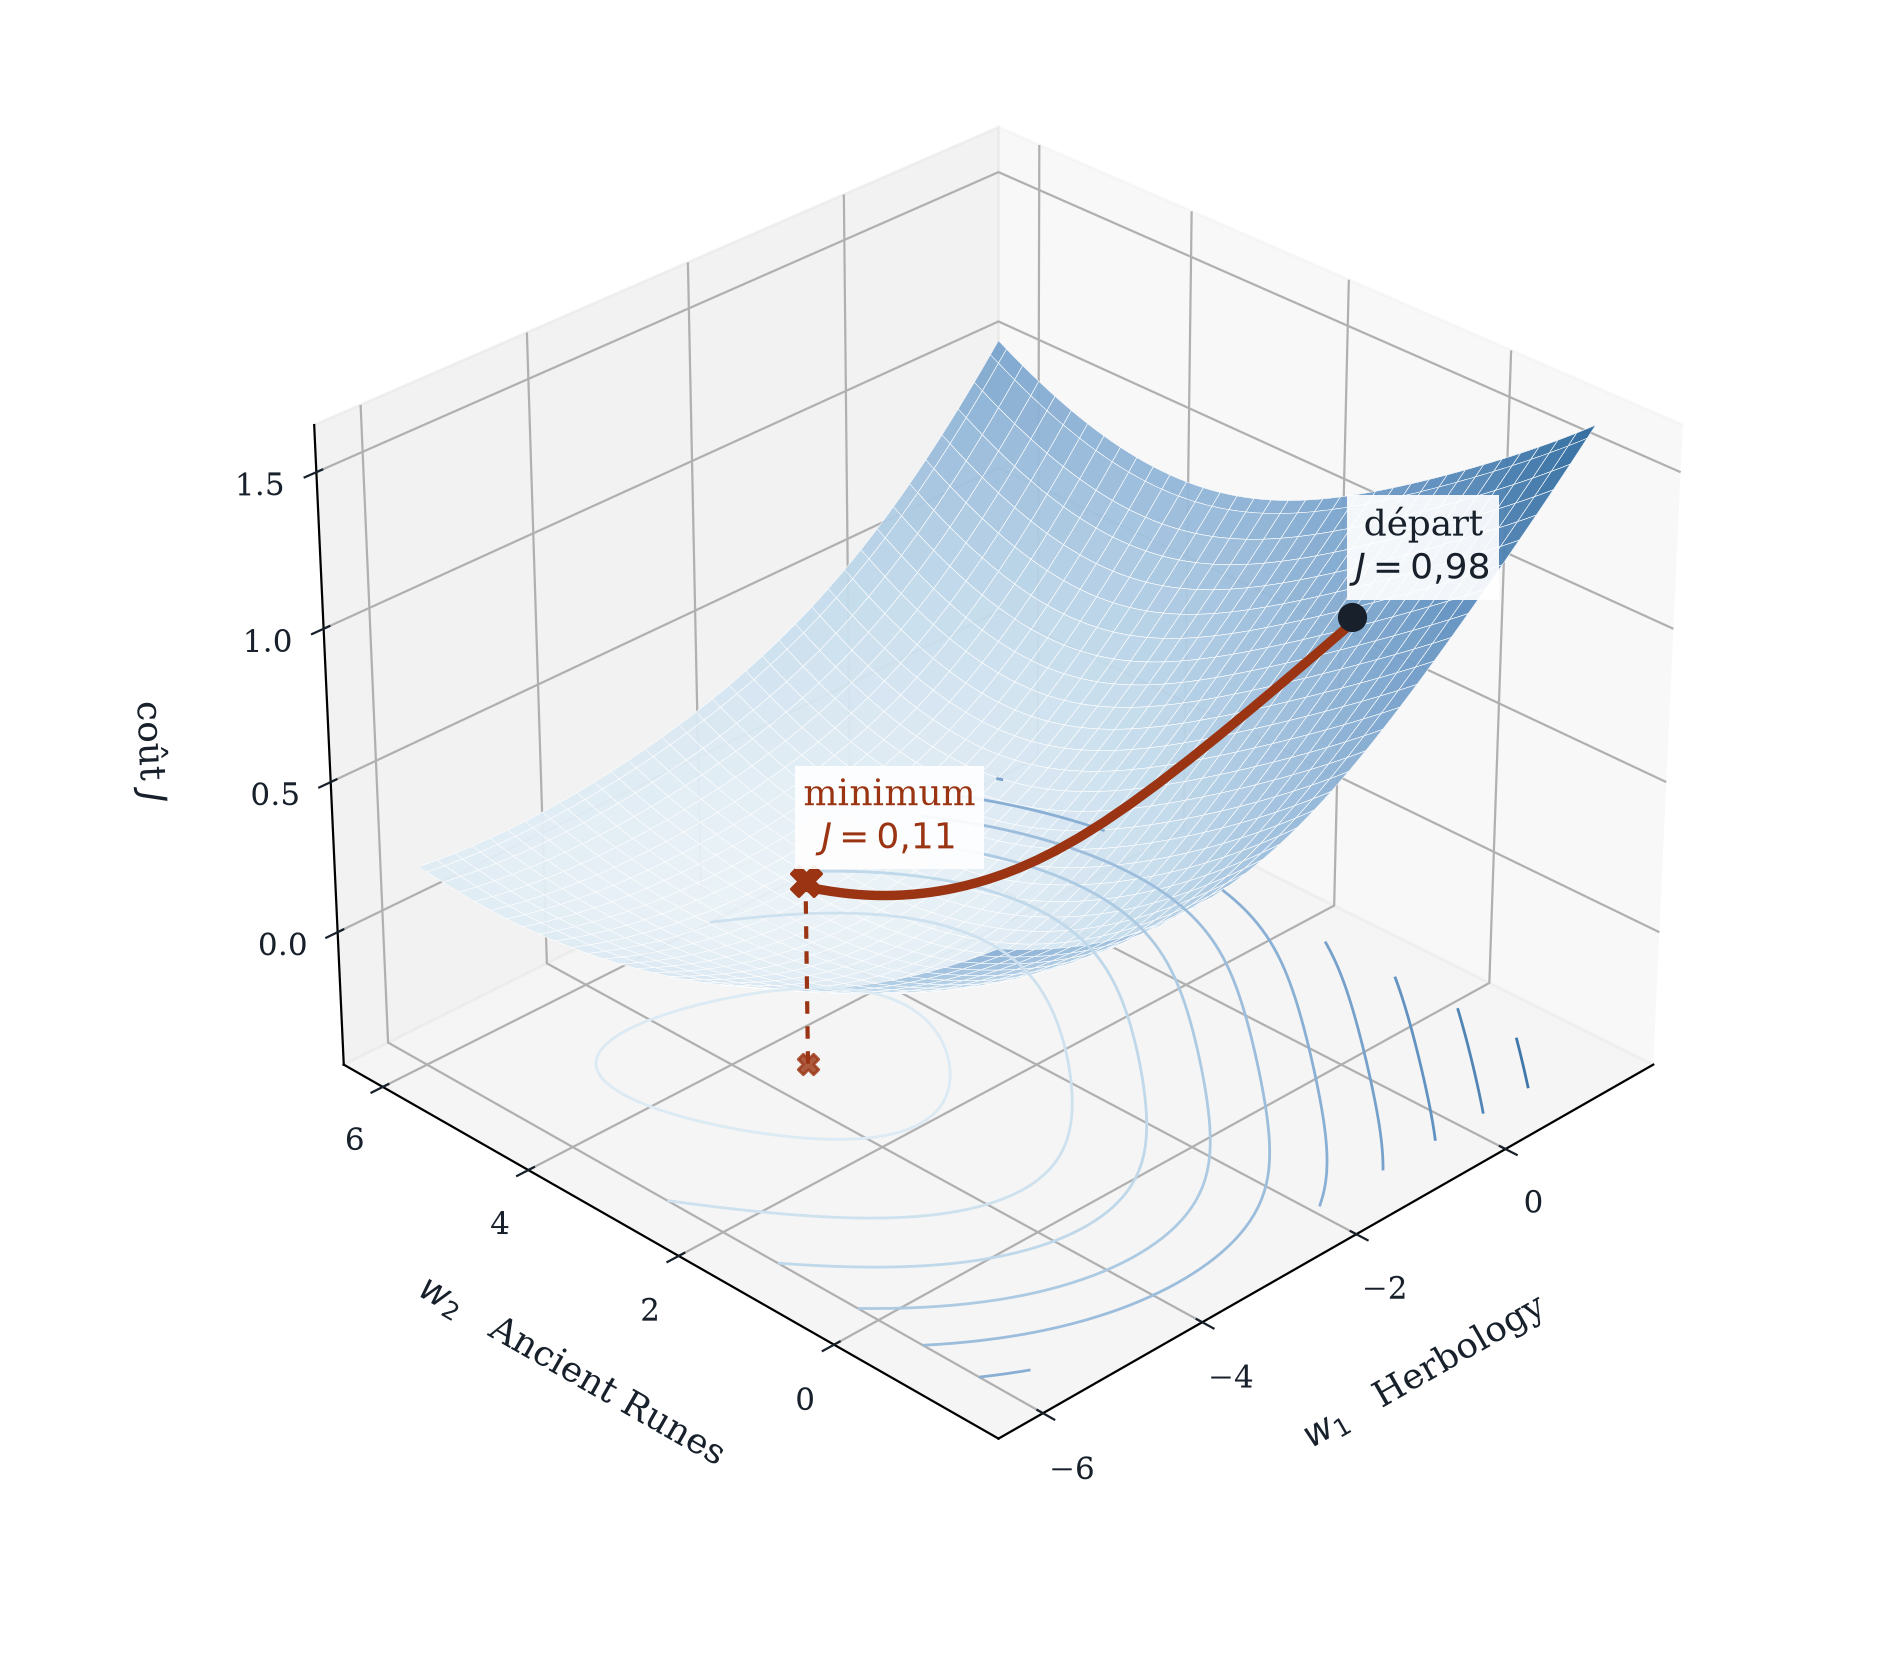
\includegraphics[width=\textwidth,
  alt={Surface tridimensionnelle de la perte moyenne au-dessus du plan des coefficients w1 et w2, en forme de cuvette allongée. Une courbe rouge descend du bord vers le fond, de 0,98 à 0,11, en coupant les lignes de niveau tracées au sol.}]{figures/surface3d.png}}
\caption{Surface de perte au-dessus du plan $(w_1,w_2)$, biais figé à
$w_0=-4{,}745$. La courbe rouge est une descente à deux coefficients exécutée
sur cette surface, de $J=0{,}98$ à $J=0{,}11$.}
\label{fig:ann-opt-surface}
\end{figure}

\begin{figure}[htbp]
\centering
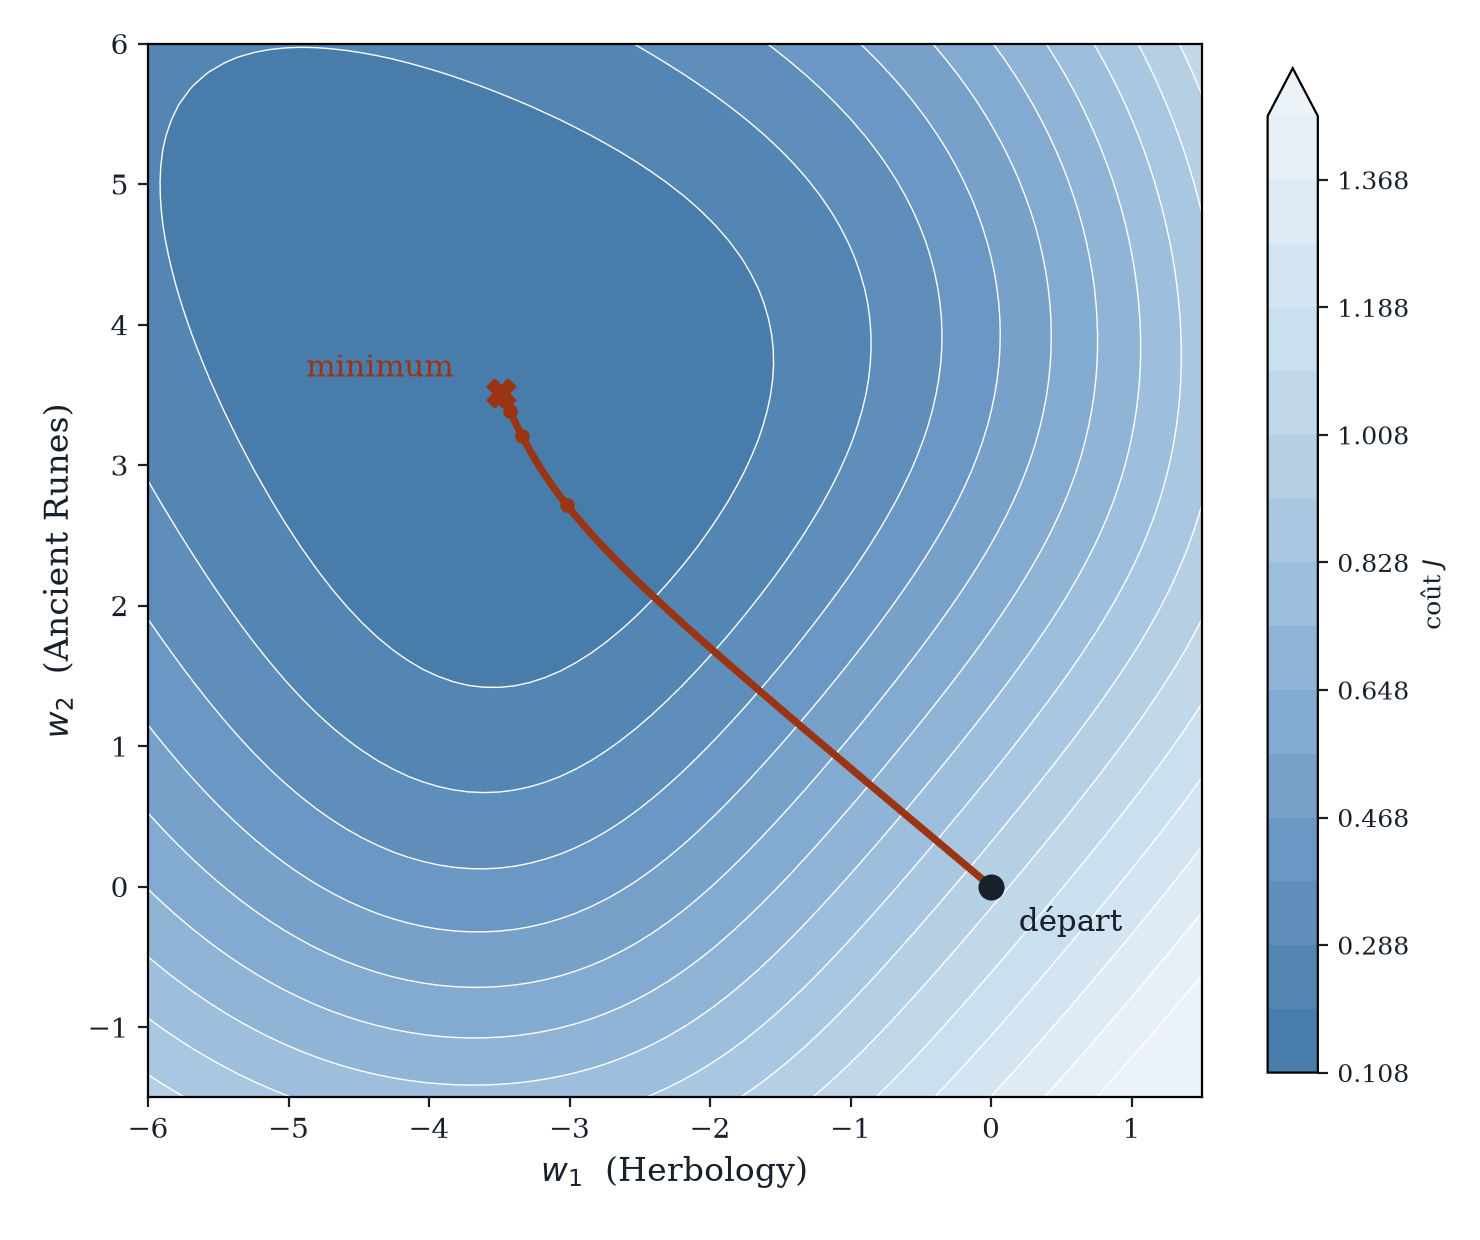
\includegraphics[width=.78\textwidth,
  alt={Lignes de niveau de la perte dans le plan des coefficients, en ellipses emboîtées. La trajectoire de descente les coupe perpendiculairement ; ses points, marqués toutes les vingt-cinq itérations, s'espacent au début et se resserrent près du fond.}]{figures/contours.png}
\caption{La même surface vue de dessus. Chaque courbe relie les couples de perte
égale ; la trajectoire les coupe perpendiculairement. Les points marquent une
itération sur vingt-cinq.}
\label{fig:ann-opt-contours}
\end{figure}
\FloatBarrier

\section{Longueur du pas}

À chaque tour, le gradient fournit une direction : son opposé $-\nabla J$ est
celle dans laquelle la perte décroît le plus vite depuis le point courant. La
distance à parcourir dans cette direction est fixée par $\alpha$. Direction et
longueur sont deux décisions séparées : la première se calcule, la seconde se
règle.

Un pas court consomme la correction disponible par fractions, et il en faut
d'autant plus de tours pour parcourir la même distance. Chaque tour demandant un
passage complet sur les $1\,600$ lignes, ce choix se paie en temps de calcul pour
aboutir à la même frontière.

Un pas long expose au dépassement. La pente que donne le gradient décrit
fidèlement le terrain au seul voisinage du point où elle est calculée. Sortir de
ce voisinage fait passer les coefficients de l'autre côté du minimum, sur la
pente opposée, et le coût augmente. Les tours suivants ramènent vers le bas, au
prix d'un détour.

\begin{figure}[htbp]
\centering
\begin{graphique}{Quatre courbes de coût sur quarante itérations. Le pas 0,05 décroît lentement et reste très au-dessus. Les pas 0,3 et 1 décroissent régulièrement. Le pas 100 descend d'abord plus vite puis présente une trajectoire heurtée avant de rejoindre le bas.}
\begin{tikzpicture}
\begin{axis}[width=.82\textwidth,height=6.8cm,
  axis lines=left,axis line style={ink!40},
  grid=major,grid style={gridgray!30},
  tick label style={font=\small},label style={font=\small},
  xlabel={itération},ylabel={coût $J$},
  xmin=0,xmax=40,ymin=0.09,ymax=0.72,
  legend style={at={(0.98,0.97)},anchor=north east,draw=none,font=\small,
    fill=white,fill opacity=0.85,text opacity=1}]
  \addplot[warning,very thick,no markers] table[x=iter,y=a005] {data/alpha.dat};
  \addlegendentry{$\alpha=0{,}05$}
  \addplot[huffle,thick,densely dashed,no markers]
    table[x=iter,y=a03] {data/alpha.dat};
  \addlegendentry{$\alpha=0{,}3$}
  \addplot[accent,very thick,no markers] table[x=iter,y=a10] {data/alpha.dat};
  \addlegendentry{$\alpha=1$}
  \addplot[slyth,thick,densely dotted,no markers]
    table[x=iter,y=a1000] {data/alpha.dat};
  \addlegendentry{$\alpha=100$}
\end{axis}
\end{tikzpicture}
\end{graphique}
\caption{Quarante itérations à partir de \Mzero, quatre réglages du pas. À
$\alpha=100$, la trajectoire est heurtée : le déplacement dépasse le minimum le
long de plusieurs directions.}
\label{fig:ann-opt-alpha-reel}
\end{figure}
\FloatBarrier

\begin{chiffres}[Perte moyenne selon le pas]
\begin{center}
\begin{tabular}{crrrl}
\toprule
$\alpha$ & départ & après un tour & après quarante & \\
\midrule
$0{,}05$ & $0{,}693147$ & $0{,}684362$ & $0{,}466848$ & pas trop court \\
$0{,}3$  & $0{,}693147$ & $0{,}642124$ & $0{,}237761$ & \\
$1$      & $0{,}693147$ & $0{,}538507$ & $0{,}153427$ & réglage retenu \\
$100$    & $0{,}693147$ & $0{,}408290$ & $0{,}111846$ & trajectoire heurtée \\
$1\,000$ & $0{,}693147$ & $4{,}049$    & --- & premier pas au-delà de la cible \\
\bottomrule
\end{tabular}
\end{center}
Les cinq réglages partent de $\log 2$, les coefficients nuls donnant $0{,}5$
partout. À $\alpha=100$, le faible gradient initial produit encore une baisse
au premier tour malgré l'amplitude du déplacement ; la trajectoire devient
ensuite heurtée. À $\alpha=1\,000$, le premier tour porte
la perte de $0{,}69$ à $4{,}05$. Le seuil se lit sur la courbe, non à l'{\oe}il.
\end{chiffres}

$\alpha$ se règle par essais, en lisant la courbe de perte : un bon réglage la
fait décroître à chaque tour, vite d'abord puis de moins en moins. Une remontée,
même isolée, indique un pas trop long. Le cours retient $\alpha=1$.

\section{Condition de décroissance}

La longueur du déplacement, $\alpha\|\nabla J\|$, croît sans borne avec $\alpha$,
et un pas suffisamment grand fait diverger la descente. Le seuil au-delà duquel
cela se produit est fixé par la courbure de $J$ par rapport aux
\emph{coefficients}, c'est-à-dire par la hessienne
$\tfrac{1}{m}\X^{\!\top}S\X$, qui fait intervenir l'échelle et les corrélations
des colonnes de $\X$ (\annexeref{ann:convexite}). La borne $p(1-p)\leq\frac14$
porte sur le seul facteur $s_i$ et laisse ce seuil indéterminé.

L'énoncé exact est conditionnel. Si le gradient de $J$ est $L$-lipschitzien ---
ce qui est le cas ici, avec $L\leq\tfrac{1}{4m}\|\X\|^2$ --- alors tout pas
$\alpha<2/L$ fait décroître $J$ à chaque tour, et $\alpha\leq1/L$ garantit une
convergence en $O(1/t)$~\cite{nocedal2006,boyd2004}. Ce seuil dépend des données,
d'où le réglage par essais plutôt que par formule.

La standardisation des colonnes (ch.~\ref{ch:standardisation}) intervient
directement : en rapprochant les échelles des colonnes, elle réduit l'écart entre
les courbures dans les différentes directions et rend un même $\alpha$ acceptable
pour tous les coefficients.

\begin{figure}[htbp]
\centering
\begin{graphique}{Deux graphiques de suites d'itérés d'une quadratique de minimum 2, ligne pointillée horizontale. À gauche, pas adapté : les points convergent vers 2 en se rapprochant à chaque tour. À droite, pas critique : les points oscillent indéfiniment entre -2 et 6.}
\begin{minipage}[t]{.48\textwidth}
\centering
\begin{tikzpicture}[alt={Suite d'itérés d'une fonction quadratique avec un pas adapté ; les points convergent vers le minimum situé en 2.}]
\begin{axis}[width=.95\linewidth,height=5.4cm,axis lines=left,
  title={$\alpha$ adapté},xlabel={itération},ylabel={$\theta$},
  xmin=0,xmax=6,ymin=-2.6,ymax=6.6,grid=major,grid style={gridgray!45}]
  \addplot[accent,very thick,mark=*] coordinates
    {(0,-2) (1,0) (2,1) (3,1.5) (4,1.75) (5,1.875) (6,1.9375)};
  \addplot[ink,dashed,thick,domain=0:6]{2};
\end{axis}
\end{tikzpicture}
\end{minipage}\hfill
\begin{minipage}[t]{.48\textwidth}
\centering
\begin{tikzpicture}[alt={Suite d'itérés de la même fonction avec le pas critique ; les points oscillent entre -2 et 6 sans converger vers le minimum situé en 2.}]
\begin{axis}[width=.95\linewidth,height=5.4cm,axis lines=left,
  title={$\alpha$ trop grand},xlabel={itération},ylabel={$\theta$},
  xmin=0,xmax=6,ymin=-2.6,ymax=6.6,grid=major,grid style={gridgray!45}]
  \addplot[warning,very thick,mark=*] coordinates
    {(0,-2) (1,6) (2,-2) (3,6) (4,-2) (5,6) (6,-2)};
  \addplot[ink,dashed,thick,domain=0:6]{2};
\end{axis}
\end{tikzpicture}
\end{minipage}
\end{graphique}
\caption{Quadratique d'une variable, courbure $c$, minimum en $2$. À gauche
$\alpha<2/c$ : convergence. À droite $\alpha=2/c$ : oscillation entre deux
valeurs ; tout $\alpha>2/c$ diverge.}
\label{fig:ann-opt-alpha-quadratique}
\end{figure}
\FloatBarrier

\begin{exercice}[Pas critique d'une quadratique]
Soit $f(\theta)=\tfrac{c}{2}(\theta-2)^2$ avec $c=4$. Écrire l'itération de
descente de gradient, en déduire la relation entre $\theta_{t+1}-2$ et
$\theta_t-2$, puis la valeur de $\alpha$ à partir de laquelle la suite cesse de
converger. Vérifier sur la
figure~\ref{fig:ann-opt-alpha-quadratique}.
\end{exercice}

\textbf{Retour au fil principal.} Le critère d'arrêt et les régimes successifs de
la descente sont au chapitre~\ref{ch:descente}, section~5.

\chapter{Réécritures pour la stabilité numérique}
\label{ch:stabilite}

\begin{lecture}
Les formules démontrées jusqu'ici sont exactes en arithmétique réelle. Sur une
machine, les nombres ont une taille finie, et deux expressions mathématiquement
égales n'y sont pas équivalentes : l'une rend un résultat, l'autre échoue. Les
deux réécritures établies ici conservent chaque valeur et modifient seulement la
suite d'opérations qui y conduit.
\end{lecture}

\section{Coût exprimé à partir du score}

En double précision, $\sigma(z)$ vaut exactement $1$ dès que $z$ dépasse environ
$37$ : $e^{-37}$ est de l'ordre de $10^{-17}$, en dessous de ce qu'un flottant
distingue de $1$ lorsqu'on l'y ajoute. Le coût demande alors $\log(1-1)$, qui
n'existe pas. Un élève d'une autre maison auquel le modèle attribue une forte
probabilité d'être \Gryf suffit donc à interrompre le programme, alors que
c'est exactement le cas que le coût doit signaler.

\begin{rappel}[Logarithme d'un quotient, logarithme d'une exponentielle]
$\log(a/b)=\log a-\log b$, et $\log(e^{b})=b$.
\end{rappel}

Reprenons le coût d'un élève et remplaçons $p$ par $\sigma(z)$ :

\begin{align}
  \ell &= -\bigl[y\log\sigma(z)+(1-y)\log(1-\sigma(z))\bigr] \notag\\[4pt]
  \log\sigma(z) &= \log\frac{1}{1+e^{-z}}
    = \log 1-\log(1+e^{-z}) \notag\\
    &= -\log(1+e^{-z})
    &&\text{car } \log 1=0 \notag\\[4pt]
  \log\bigl(1-\sigma(z)\bigr) &= \log\frac{e^{-z}}{1+e^{-z}}
    = \log e^{-z}-\log(1+e^{-z}) \notag\\
    &= -z-\log(1+e^{-z})
    &&\text{car } \log e^{-z}=-z \notag\\[4pt]
  \ell &= -\Bigl[y\bigl(-\log(1+e^{-z})\bigr) \notag\\
    &\qquad\quad +(1-y)\bigl(-z-\log(1+e^{-z})\bigr)\Bigr] \notag\\[4pt]
  &= y\log(1+e^{-z})+(1-y)z+(1-y)\log(1+e^{-z})
    &&\text{on distribue} \notag\\[4pt]
  &= \log(1+e^{-z})+(1-y)z
    &&\text{les logs se regroupent} \notag\\[4pt]
  &= \underbrace{\log(1+e^{-z})+z}_{=\;\log(1+e^{z})}-yz \notag\\[4pt]
  &= \log(1+e^{z})-yz
\end{align}

Le regroupement souligné s'établit ainsi :
\[
  \log(1+e^{-z})+z
  = \log(1+e^{-z})+\log e^{z}
  = \log\bigl(e^{z}(1+e^{-z})\bigr)
  = \log(e^{z}+1),
\]
en remontant $z$ sous forme de $\log e^{z}$, en regroupant les deux logarithmes
en celui d'un produit, puis en développant : $e^{z}\cdot e^{-z}=e^{0}=1$.

\begin{resultat}[Forme employée par le programme]
\[
  \ell(y,z)=\operatorname{softplus}(z)-yz,
  \qquad \operatorname{softplus}(z)=\log(1+e^{z}).
\]
Cette forme se calcule à partir du score seul, hors d'atteinte des arrondis qui
produisent $\log 0$.
\end{resultat}

\begin{releve}
Pour $y=1$ et $z=6$, la forme directe donne $-\log(0{,}997527)=0{,}002476$ et
celle-ci $\operatorname{softplus}(6)-6=6{,}002476-6=0{,}002476$.
\end{releve}

\section{Formes protégées de softplus et de la sigmoïde}

$\operatorname{softplus}$ contient encore $e^{z}$, qui déborde pour $z$ grand.
On l'écrit donc
\[
  \operatorname{softplus}(z)=\max(z,0)+\log\bigl(1+e^{-|z|}\bigr),
\]
dont l'exposant est toujours négatif ou nul. La vérification porte sur deux cas.
Pour $z\geq0$, $\max(z,0)=z$ et l'expression vaut
$z+\log(1+e^{-z})=\log(e^{z}+1)$, par le même regroupement que ci-dessus. Pour
$z<0$, $\max(z,0)=0$ et $|z|=-z$, il reste $\log(1+e^{z})$, qui est la
définition.

La sigmoïde reçoit le même traitement, avec ses deux écritures
(ch.~\ref{ch:logit}) :
\[
  \sigma(z)=
  \begin{cases}
    1/(1+e^{-z}), & z\geq 0,\\[2pt]
    e^{z}/(1+e^{z}), & z<0 .
  \end{cases}
\]
Dans les deux branches, l'exponentielle porte sur un nombre négatif ou nul. Un
exposant très négatif s'arrondit à zéro sans dommage ; un exposant très positif dépasse en revanche la capacité du format et provoque une erreur.

\begin{figure}[htbp]
\centering
\begin{tikzpicture}[font=\small,x=0.0083cm]
% Axe des scores, de -900 a 900 ; 1 unite = 0,0083 cm, soit 14,9 cm au total.
\fill[warning!18] (-900,-0.28) rectangle (-710,0.28);
\fill[warning!18] (710,-0.28) rectangle (900,0.28);
\fill[huffle!12] (37,-0.28) rectangle (710,0.28);
\fill[huffle!12] (-710,-0.28) rectangle (-37,0.28);
\fill[rulecolor!12] (-37,-0.28) rectangle (37,0.28);
\draw[ink!45] (-900,0) -- (900,0);
\foreach \v in {-800,-400,0,400,800}{
  \draw[ink!45] (\v,-0.32) -- (\v,0.32);
  \node[font=\scriptsize,text=ink,anchor=north] at (\v,-0.36) {$\v$};
}
\foreach \v/\lab in {-710/{$-710$},-37/{$-37$},37/{$37$},710/{$710$}}{
  \draw[ink!60,thin] (\v,-0.28) -- (\v,0.28);
  \node[font=\scriptsize,text=ink!75,anchor=south] at (\v,0.32) {\lab};
}
\node[font=\footnotesize,text=ink,anchor=north] at (0,-1.0) {score $z$};
\node[font=\scriptsize,text=rulecolor,align=center,anchor=north]
  at (0,-1.6) {$\sigma$ et $\log$\\ exacts};
\node[font=\scriptsize,text=huffle,align=center,anchor=north]
  at (370,-1.6) {$\sigma$ arrondie à $0$ ou $1$ :\\ $\log$ direct impossible};
\node[font=\scriptsize,text=huffle,align=center,anchor=north]
  at (-370,-1.6) {$\sigma$ arrondie à $0$ ou $1$ :\\ $\log$ direct impossible};
\node[font=\scriptsize,text=warning,align=center,anchor=north]
  at (805,-1.6) {$e^{|z|}$\\ déborde};
\node[font=\scriptsize,text=warning,align=center,anchor=north]
  at (-805,-1.6) {$e^{|z|}$\\ déborde};
\end{tikzpicture}
\caption{Les trois régimes du calcul en double précision. La zone centrale seule
tolère l'écriture directe ; les formes protégées rendent des valeurs finies sur
tout l'axe. Un score de $\pm800$ apparaît dès que les coefficients divergent
(ch.~\ref{ch:convexite}).}
\label{fig:regimes}
\end{figure}
\FloatBarrier

\begin{table}[htbp]
\centering
\begin{tabular}{rll}
\toprule
$z$ & écriture directe & écriture protégée \\
\midrule
$-800$ & $e^{800}$ déborde & $0{,}0$ \\
$+800$ & $\log(1+e^{800})$ déborde & $800{,}0$ \\
$+40$  & $\log(1-\sigma(40))=\log 0$ & $0{,}0$ \\
\bottomrule
\end{tabular}
\caption{En double précision, l'exponentielle déborde au-delà de
$|z|\approx710$ et la sigmoïde s'arrondit à $1$ dès $z\approx37$. Les formes
protégées rendent des valeurs finies dans les trois cas.}
\label{tab:stabilite}
\end{table}

\begin{vigilance}[Contrôles numériques]
Le premier coût vaut $\log 2=0{,}693147$ quand les coefficients partent de zéro.
Toute autre valeur signale une erreur dans le score ou l'initialisation.

Le gradient calculé par la formule, comparé à
$\bigl(J(\w+h\mathbf e_j)-J(\w-h\mathbf e_j)\bigr)/2h$ sur un cas de petite
taille, doit coïncider à $10^{-6}$ près. Ce test détecte un signe inversé, un
facteur $1/m$ oublié, un indice décalé.

La sigmoïde et le coût, évalués en $z=\pm1000$, doivent rendre des nombres finis.
\end{vigilance}

% !TeX root = ../regression_logistique.tex
\chapter{Géométrie en dimension quelconque}
\label{ann:geometrie}

\orient{%
écrire l'équation d'une frontière pour $n$ variables et en donner la dimension ;
décrire la région attribuée à une classe par la règle du maximum et énoncer ses
propriétés exactes}{%
produit scalaire et norme (\annexeref{ann:prerequis}) ; chapitres~\ref{ch:nuage}
et~\ref{ch:classifieur}}{%
approfondissement ; se saute sans rompre la lecture du fil principal}

\section{Frontière pour un nombre quelconque de matières}

Avec $n$ notes, une observation est un point de $\R^n$ et l'équation de la
frontière devient
\[
  w_0+w_1x_1+\dots+w_nx_n=0,
\]
soit une équation linéaire à $n$ inconnues, non triviale dès que
$(w_1,\dots,w_n)\neq0$. Son ensemble de solutions est un sous-espace affine de
dimension $n-1$ : une contrainte non dégénérée retire un degré de liberté. Cet
objet porte le nom d'\emph{hyperplan affine} de $\R^n$ --- droite pour $n=2$,
plan pour $n=3$, sans représentation graphique au-delà.

\begin{table}[htbp]
\centering
\begin{tabular}{ccccc}
\toprule
matières & espace des observations & frontière & sa dimension & coefficients \\
\midrule
$1$  & $\R$      & un point    & $0$ & $2$  \\
$2$  & $\R^2$    & une droite  & $1$ & $3$  \\
$3$  & $\R^3$    & un plan     & $2$ & $4$  \\
$n$  & $\R^n$    & un hyperplan & $n-1$ & $n+1$ \\
\midrule
$10$ & $\R^{10}$ & un hyperplan & $9$ & $11$ \\
\bottomrule
\end{tabular}
\caption{La frontière occupe une dimension de moins que l'espace des
observations et le sépare en deux demi-espaces. Le nombre de coefficients croît
d'une unité par matière ajoutée.}
\label{tab:dimensions}
\end{table}

\begin{figure}[htbp]
\centering
\begin{graphique}{Trois vignettes. Pour une matière, un axe portant un point qui sépare disques et croix. Pour deux matières, un rectangle traversé par une droite. Pour trois matières, un repère en perspective traversé par un plan. Les dimensions 0, 1 et 2 sont indiquées sous chacune.}
\begin{tikzpicture}[baseline=(current bounding box.north),font=\footnotesize,
  alt={En dimension un, un point sur un axe sépare les observations des deux classes.}]
\node[font=\small,anchor=south] at (1.6,1.5) {$n=1$};
\draw[ink!45] (0,0.4) -- (3.2,0.4);
\foreach \x in {0.3,0.6,0.95,1.25}{\fill[accent] (\x,0.4) circle (1.5pt);}
\foreach \x in {1.95,2.25,2.6,2.95}{
  \draw[warning!80,line width=.7pt] (\x-.06,0.34) -- (\x+.06,0.46);
  \draw[warning!80,line width=.7pt] (\x-.06,0.46) -- (\x+.06,0.34);}
\fill[ink] (1.6,0.4) circle (2.2pt);
\node[anchor=north,text=ink] at (1.6,0.25) {un point};
\node[anchor=north,text=ink!70,font=\scriptsize] at (1.6,-0.15)
  {dimension $0$};
\end{tikzpicture}\hfill
\begin{tikzpicture}[baseline=(current bounding box.north),font=\footnotesize,
  alt={En dimension deux, une droite dans un plan sépare les observations des deux classes.}]
\node[font=\small,anchor=south] at (1.6,1.5) {$n=2$};
\draw[gridgray!60] (0,-0.35) rectangle (3.2,1.35);
\draw[ink,very thick] (0.25,-0.1) -- (2.95,1.1);
\foreach \p in {(0.6,0.9),(1.0,1.15),(1.5,1.25)}{\fill[accent] \p circle (1.5pt);}
\foreach \p/\qx/\qy in {(1.5,0.1)/1.5/0.1,(2.2,0.35)/2.2/0.35,(2.6,0.15)/2.6/0.15}{
  \draw[warning!80,line width=.7pt] (\qx-.06,\qy-.06) -- (\qx+.06,\qy+.06);
  \draw[warning!80,line width=.7pt] (\qx-.06,\qy+.06) -- (\qx+.06,\qy-.06);}
\node[anchor=north,text=ink] at (1.6,-0.45) {une droite};
\node[anchor=north,text=ink!70,font=\scriptsize] at (1.6,-0.85)
  {dimension $1$};
\end{tikzpicture}\hfill
\begin{tikzpicture}[baseline=(current bounding box.north),font=\footnotesize,
  alt={En dimension trois, un plan dans l'espace sépare les observations des deux classes.}]
\node[font=\small,anchor=south] at (1.6,1.5) {$n=3$};
\draw[ink!45,-{Latex[length=1.6mm]}] (0.9,0.3) -- (2.9,0.3);
\draw[ink!45,-{Latex[length=1.6mm]}] (0.9,0.3) -- (1.6,0.85);
\draw[ink!45,-{Latex[length=1.6mm]}] (0.9,0.3) -- (0.9,1.4);
\fill[ink!22,draw=ink!60] (0.35,0.45) -- (2.35,-0.15) -- (2.95,0.55)
  -- (0.95,1.15) -- cycle;
\foreach \p in {(1.1,0.95),(1.7,0.8)}{\fill[accent] \p circle (1.5pt);}
\foreach \qx/\qy in {1.6/0.15,2.3/0.35}{
  \draw[warning!80,line width=.7pt] (\qx-.06,\qy-.06) -- (\qx+.06,\qy+.06);
  \draw[warning!80,line width=.7pt] (\qx-.06,\qy+.06) -- (\qx+.06,\qy-.06);}
\node[anchor=north,text=ink] at (1.6,-0.45) {un plan};
\node[anchor=north,text=ink!70,font=\scriptsize] at (1.6,-0.85)
  {dimension $2$};
\end{tikzpicture}
\end{graphique}
\caption{Frontière pour une, deux et trois matières. Disque : classe traitée ;
croix : autres classes. Le vecteur normal, $|z|/\|w\|$ et le signe de $z$
conservent leur rôle.}
\label{fig:dimensions}
\end{figure}
\FloatBarrier

Les formules du fil principal s'écrivent avec un nombre quelconque de notes, et
les démonstrations des annexes suivantes valent pour $n$ quelconque. Deux
matières servent en partie~I parce qu'elles se dessinent ; le modèle complet du
projet en retient dix.

\section{Rôle de chaque coefficient}

Les trois coefficients agissent séparément : $(w_1,w_2)$ fixe la direction de la
frontière et $w_0$ sa position. La norme $\|w\|$ laisse la frontière en place et
fixe la vitesse à laquelle $z$ croît lorsqu'on s'en éloigne
(ch.~\ref{ch:descente}).

\begin{figure}[htbp]
\centering
\begin{graphique}{Un plan quadrillé traversé par une droite oblique séparant deux demi-plans teintés, marqués z positif et z négatif. Depuis le pied de la perpendiculaire issue de l'origine part un vecteur normal ; un segment nommé d indice O joint l'origine à ce pied.}
\begin{tikzpicture}
\begin{axis}[width=.66\textwidth,axis equal image,
  axis lines=box,axis line style={ink!40},
  grid=major,grid style={gridgray!25},
  tick label style={font=\small},label style={font=\small},
  xlabel={$x_1$},ylabel={$x_2$},
  xmin=-2.2,xmax=2.2,ymin=-1.4,ymax=2.2,
  xtick={-2,-1,0,1,2},ytick={-1,0,1,2},
  domain=-2.2:2.2,samples=2,clip=true]

  \fill[accent!12] (axis cs:-2.2,-0.92) -- (axis cs:2.2,1.72)
    -- (axis cs:2.2,2.2) -- (axis cs:-2.2,2.2) -- cycle;
  \fill[warning!10] (axis cs:-2.2,-0.92) -- (axis cs:2.2,1.72)
    -- (axis cs:2.2,-1.4) -- (axis cs:-2.2,-1.4) -- cycle;

  \addplot[ink,very thick]{0.4+0.6*x};

  % angle droit entre la frontiere et sa normale, au pied H
  \addplot[ink!70,thin] coordinates
    {(-0.022,0.387) (-0.115,0.541) (-0.269,0.448)};

  \addplot[warning,-{Latex[length=2.6mm]},very thick]
    coordinates {(-0.176,0.294) (-0.776,1.294)};
  \addplot[accent,very thick] coordinates {(0,0) (-0.176,0.294)};
  \addplot[only marks,mark=*,ink,mark size=2pt]
    coordinates {(0,0) (-0.176,0.294)};

  \node[font=\small,text=accent,anchor=east] at (axis cs:-0.20,0.16) {$d_O$};

  \node[font=\small,text=warning,anchor=south] at (axis cs:-0.776,1.36)
    {$(w_1,w_2)$};
  \node[font=\scriptsize,text=ink,anchor=north east] at (axis cs:-0.05,-0.04)
    {$O$};
  \node[font=\small,text=ink,fill=white,inner sep=1.5pt,anchor=south east]
    at (axis cs:2.12,1.70) {$z=0$};
  \node[font=\small,text=accent!80!black,anchor=north west]
    at (axis cs:-2.08,2.12) {$z>0$};
  \node[font=\small,text=warning,anchor=south east]
    at (axis cs:2.08,-1.32) {$z<0$};
\end{axis}
\end{tikzpicture}
\end{graphique}
\caption{Frontière $-0{,}4-0{,}6x_1+x_2=0$ et son vecteur normal
$(-0{,}6\,;1)$, tracé à l'échelle depuis le pied de la perpendiculaire issue de
l'origine. Le segment $d_O$ mesure $-w_0/\|w\|=0{,}343$.}
\label{fig:normal}
\end{figure}
\FloatBarrier

Les deux panneaux suivants font varier un coefficient à la fois à partir de
$w=(0\,;0{,}8\,;1)$. Ils couvrent tous les cas : la frontière ne dépend que de la
direction de $(w_1,w_2)$, et faire varier $w_1$ à $w_2$ fixé parcourt cette
direction tout entière.

\begin{figure}[htbp]
\centering
\begin{graphique}{Deux panneaux. À gauche, trois droites parallèles correspondant à trois valeurs du biais. À droite, trois droites concourantes à l'origine correspondant à trois valeurs du premier coefficient. Le trait plein est commun aux deux panneaux.}
\begin{tikzpicture}[baseline=(current bounding box.north),
  alt={Trois frontières parallèles obtenues en faisant varier le biais, les deux autres coefficients restant fixes.}]
\begin{axis}[panel,width=.40\textwidth,height=5.6cm,
  title={variation de $w_0$\\[-1pt] \scriptsize $w_1=0{,}8$,\ $w_2=1$},
  title style={align=center},xlabel={$x_1$},ylabel={$x_2$},
  legend style={at={(0.5,-0.32)},anchor=north,draw=none,font=\scriptsize,
    cells={anchor=west},row sep=-1.5pt,legend image post style={scale=.7}},
  domain=-3:3,samples=2]
  \addplot[ink!45,thick,densely dashed]{-0.8*x+1.6};
  \addlegendentry{$w_0=-1{,}6$}
  \addplot[accent,very thick]{-0.8*x};
  \addlegendentry{$w_0=0$}
  \addplot[warning,thick,densely dotted]{-0.8*x-1.6};
  \addlegendentry{$w_0=+1{,}6$}
\end{axis}
\end{tikzpicture}\hfill
\begin{tikzpicture}[baseline=(current bounding box.north),
  alt={Trois frontières concourantes à l'origine obtenues en faisant varier le premier coefficient, le biais restant nul.}]
\begin{axis}[panel,width=.40\textwidth,height=5.6cm,
  title={variation de $w_1$\\[-1pt] \scriptsize $w_0=0$,\ $w_2=1$},
  title style={align=center},xlabel={$x_1$},yticklabels={},
  legend style={at={(0.5,-0.32)},anchor=north,draw=none,font=\scriptsize,
    cells={anchor=west},row sep=-1.5pt,legend image post style={scale=.7}},
  domain=-3:3,samples=2]
  \addplot[ink!45,thick,densely dashed]{-0.2*x};
  \addlegendentry{$w_1=0{,}2$}
  \addplot[accent,very thick]{-0.8*x};
  \addlegendentry{$w_1=0{,}8$}
  \addplot[warning,thick,densely dotted]{-2.2*x};
  \addlegendentry{$w_1=2{,}2$}
\end{axis}
\end{tikzpicture}
\end{graphique}
\caption{Trait plein commun aux deux panneaux : $w=(0\,;0{,}8\,;1)$. À gauche,
$w_0$ translate la droite ; à droite, $w_1$ la fait pivoter autour de l'origine,
que $w_0=0$ laisse sur la frontière.}
\label{fig:trois-nombres}
\end{figure}
\FloatBarrier

\section{Forme des régions du classifieur}

La règle du score maximal (ch.~\ref{ch:classifieur}) attribue une classe à
chaque point du plan. Quelle forme prend l'ensemble des points attribués à une
classe donnée ?

Prenons \Gryf. Son modèle l'emporte en un point lorsque son score y dépasse les
trois autres, ce qui fait trois conditions. La première s'écrit
\[
  z_G\geq z_H
  \iff
  (w_{G0}-w_{H0})+(w_{G1}-w_{H1})x_1+(w_{G2}-w_{H2})x_2\geq 0 ,
\]
et les deux autres s'obtiennent en remplaçant $H$ par $R$ puis par $S$. Le membre
de gauche est une fonction affine des deux notes ; l'inégalité définit donc un
demi-plan, bordé par la droite où les deux scores s'égalisent.

\begin{figure}[htbp]
\centering
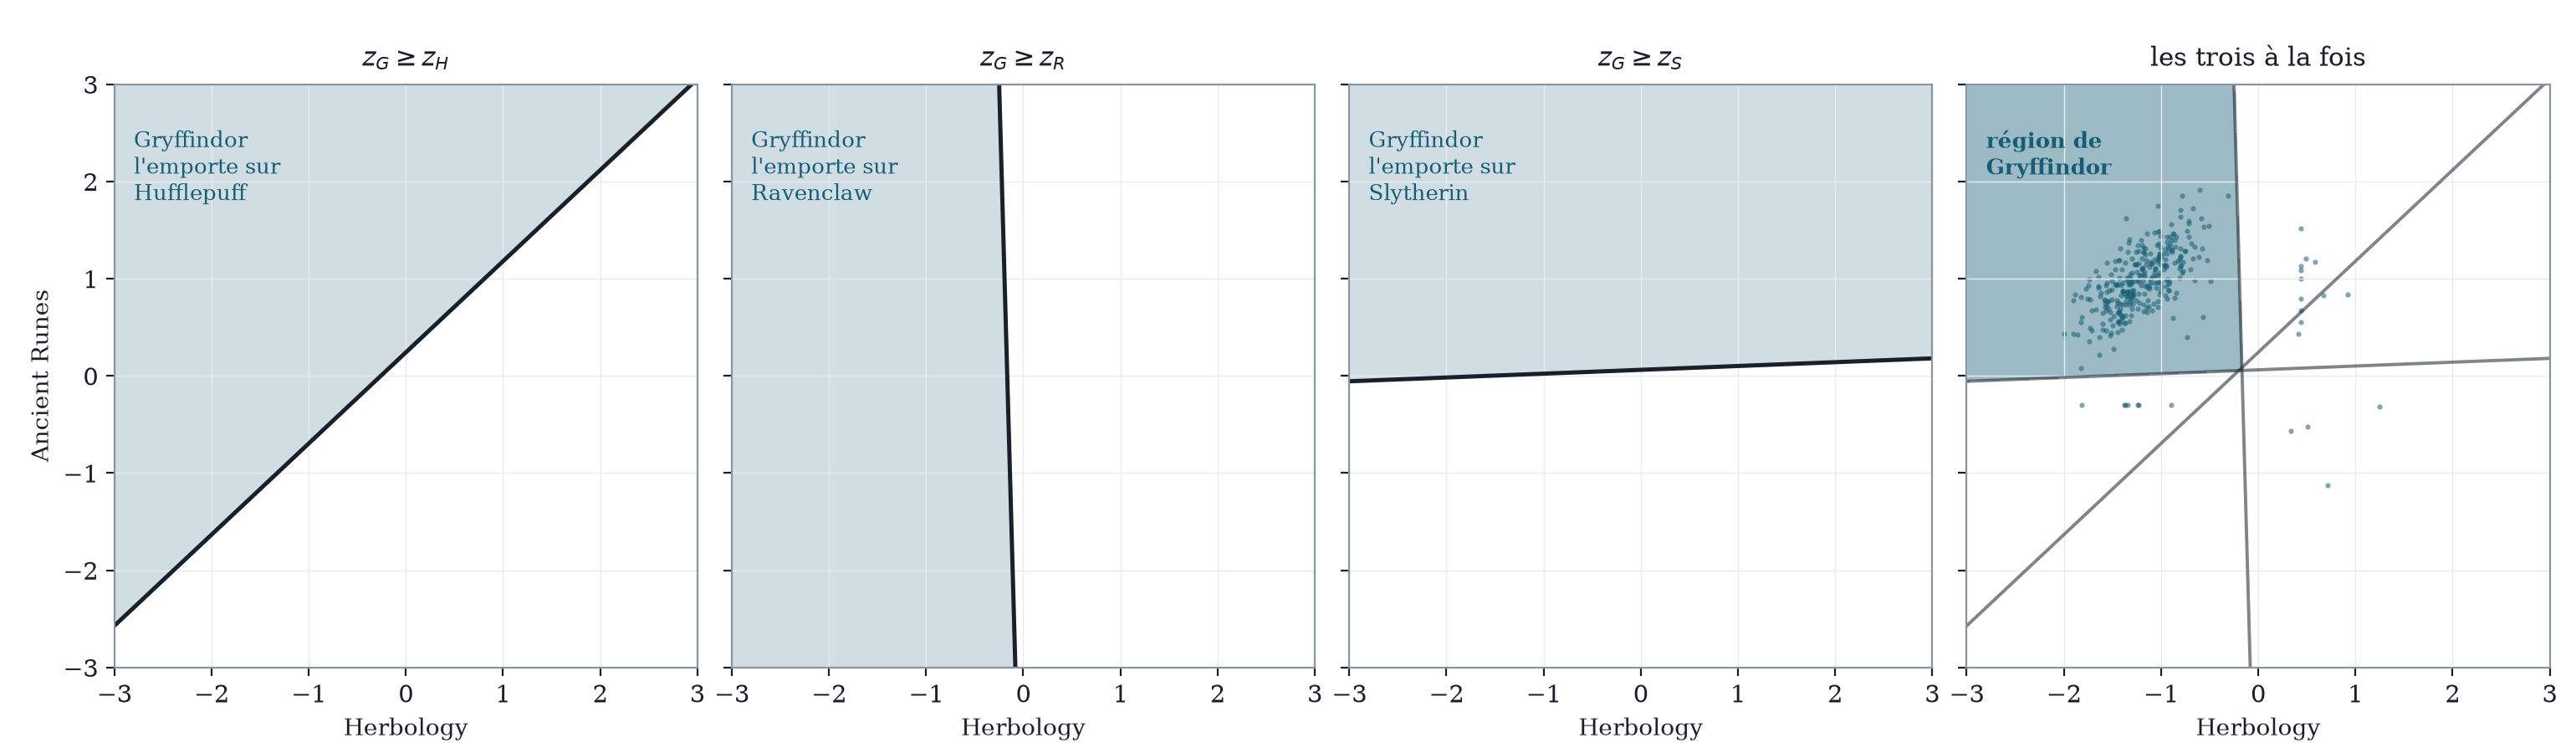
\includegraphics[width=\textwidth,
  alt={Quatre panneaux. Les trois premiers montrent chacun le demi-plan où le score de Gryffindor dépasse celui d'un rival. Le quatrième montre leur intersection, un polygone convexe non borné contenant presque toutes les observations de cette classe.}]{figures/demiplans.png}
\caption{Les trois demi-plans où \Gryf l'emporte sur chacun de ses rivaux, puis
leur intersection. Le dernier panneau porte les observations de cette classe,
qui s'y trouvent presque toutes. État du modèle : \Movr.}
\label{fig:demiplans}
\end{figure}
\FloatBarrier

La région de \Gryf est l'intersection de ces trois demi-plans : un ensemble
convexe, intersection finie de demi-plans, donc un polyèdre convexe du plan. Il
peut être vide, borné ou non borné. Trois propriétés en découlent, énoncées avec
leurs conditions.

\begin{enumerate}
  \item \textbf{Convexité.} Deux points d'une même région ont tout le segment
        qui les joint dans cette région. Une classe ne peut donc pas occuper
        deux zones séparées.
  \item \textbf{Bords.} Les bords sont portés par les droites d'égalité
        $z_G=z_j$, distinctes des quatre frontières binaires $z_k=0$. Un bord
        s'interrompt là où un troisième modèle prend le dessus. Si la région est
        bornée, ses arêtes sont de longueur finie ; si elle ne l'est pas ---
        ce qui arrive dès que la région contient une demi-droite --- au moins
        une arête est infinie. Sur les quatre modèles employés ici, les quatre
        régions sont non bornées.
  \item \textbf{Départage.} En cas d'égalité exacte entre deux scores maximaux,
        $\arg\max$ ne désigne pas une classe : il faut une convention. Le code
        de la partie~II retient le premier maximum rencontré dans l'ordre de la
        liste des classes. Cet événement est de probabilité nulle sur des
        données continues, mais se produit sur des valeurs arrondies.
\end{enumerate}

\begin{figure}[htbp]
\centering
\begin{graphique}{Un plan quadrillé traversé par trois droites : la frontière de Gryffindor en trait plein, celle de Ravenclaw en tireté, et en trait épais la limite entre leurs deux régions, presque verticale, portant son vecteur normal. Les trois se coupent en un même point.}
\begin{tikzpicture}[x=1.28cm,y=1.28cm,font=\footnotesize]
\begin{scope}
\clip (-3,-3) rectangle (3,3);
\fill[gryff!7]  (-3,-3) -- (-0.082,-3) -- (-0.248,3) -- (-3,3) -- cycle;
\fill[raven!7]  (-0.082,-3) -- (3,-3) -- (3,3) -- (-0.248,3) -- cycle;
\draw[gridgray!35] (-3,-3) grid[step=1] (3,3);
\draw[gryff,very thick] (-3,-1.611) -- (3,4.343);
\draw[raven,very thick,densely dashed] (-3,4.114) -- (3,-2.186);
\draw[ink,ultra thick] (-0.082,-3) -- (-0.248,3);
\draw[ink,-{Stealth[length=2.4mm]},thick]
  (-0.197,1.171) -- ++(-0.99,-0.028);
\end{scope}
\draw[ink!45] (-3,-3) rectangle (3,3);
\draw[ink!45] (-3,0) -- (3,0);   \draw[ink!45] (0,-3) -- (0,3);
\fill[white] (-0.197,1.171) circle (2.1pt);
\draw[ink,thick] (-0.197,1.171) circle (2.1pt);
\node[gryff,anchor=west,fill=white,inner sep=1pt] at (-2.95,-1.95) {$z_G=0$};
\node[raven,anchor=east,fill=white,inner sep=1pt] at (2.95,-1.95) {$z_R=0$};
\node[ink,anchor=south,fill=white,inner sep=1.5pt] at (-0.16,3.02)
  {$z_G=z_R$};
\node[ink,anchor=south east,font=\scriptsize] at (-1.20,1.22)
  {$w_G-w_R$};
\node[gryff!85,anchor=west] at (-2.9,2.3) {$z_G>z_R$};
\node[raven!85,anchor=east] at (2.9,2.3) {$z_R>z_G$};
\node[anchor=north] at (0,-3.15) {\Herb};
\node[anchor=south,rotate=90] at (-3.15,0) {\Runes};
\end{tikzpicture}
\end{graphique}
\caption{Frontières binaires de \Gryf (trait plein) et de \Rav (tireté), et limite entre
leurs deux régions (trait épais). Cette limite a pour vecteur normal $w_G-w_R$
et passe par l'intersection des deux premières.}
\label{fig:limite-paire}
\end{figure}
\FloatBarrier

Quatre classes forment six paires, donc six droites d'égalité, dont chacune ne
borde une région que sur la portion où le score commun aux deux classes dépasse
aussi les deux autres.

Cette construction se vérifie le long d'un trajet : chaque score y devient une
fonction affine du chemin parcouru, donc une droite, et le maximum des quatre
une ligne brisée dont les points anguleux marquent les changements de région.

\begin{figure}[htbp]
\centering
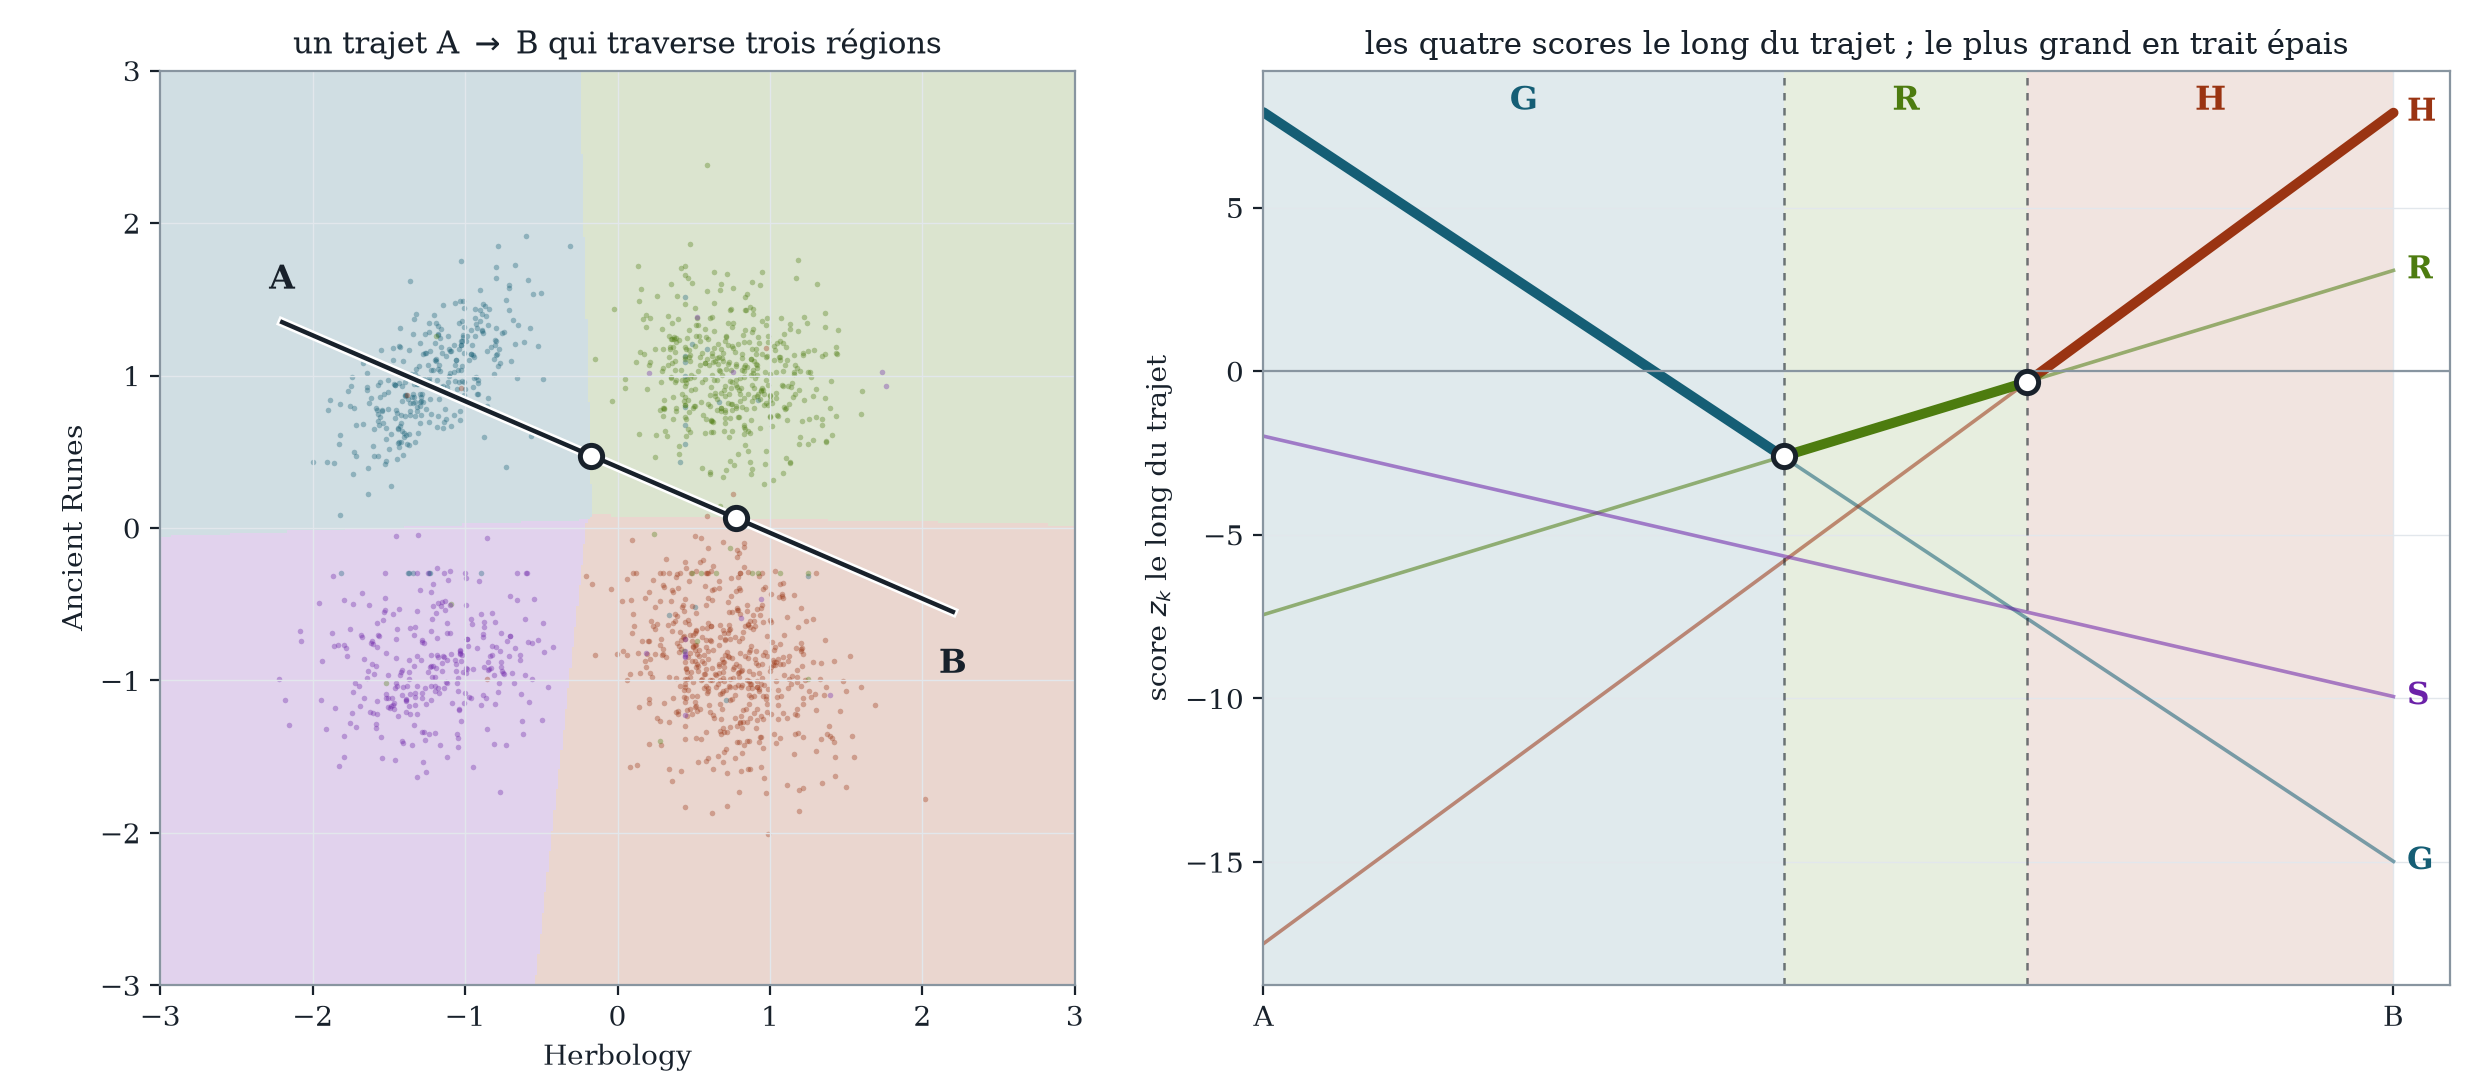
\includegraphics[width=\textwidth,
  alt={À gauche, un segment tracé dans le nuage du groupe des Gryffindor vers celui des Hufflepuff. À droite, les quatre scores relevés le long de ce segment, quatre droites ; leur maximum forme une ligne brisée à deux points anguleux marquant les changements de région.}]{figures/score_max.png}
\caption{Trajet de \Gryf vers \Huff, à gauche ; quatre scores et leur maximum, à
droite. Les angles de la ligne épaisse marquent les changements de région.}
\label{fig:score-max}
\end{figure}
\FloatBarrier

% !TeX root = ../regression_logistique.tex
\chapter{Corrigés}
\label{ann:corriges}

\orient{%
comparer une tentative au code de référence et aux réponses attendues}{%
la tâche correspondante a été tentée}{%
à consulter après avoir écrit puis exécuté sa propre version}

Cette annexe porte le code des douze tâches du cahier pratique et les réponses
aux exercices du fil principal. Chaque section porte le nom du fichier ou le
numéro de l'exercice qu'elle corrige.

\section{Cahier pratique}

\subsection*{\texttt{step0\_prepare.py} --- préparation des données}

\codefile[firstline=13,lastline=39]{scripts/tuto/step0_prepare.py}

\textbf{Transfert.} Avec $40\,\%$ de valeurs absentes, la médiane reste une
statistique correcte de la colonne observée, mais l'écart-type calculé après
imputation s'effondre : $40\,\%$ des lignes reçoivent exactement la même valeur.
Le nuage montrerait une barre verticale dense à l'abscisse de la médiane, et le
coefficient de cette variable serait tiré par un groupe artificiel.

\subsection*{\texttt{step1\_score.py} --- le score}

\codefile[firstline=4,lastline=8]{scripts/tuto/step1_score.py}

\textbf{Transfert.} Sans colonne de $1$, le gradient (ch.~\ref{ch:entrainer})
devrait traiter $\partial J/\partial w_0$ à part, avec $x_{i0}$ implicitement
égal à $1$ ; \texttt{one\_step} et \texttt{descend} hériteraient du même cas
particulier, et l'extension à dix matières multiplierait les branches.

\subsection*{\texttt{step2\_sigmoid.py} --- la sigmoïde protégée}

\codefile[firstline=4,lastline=7]{scripts/tuto/step2_sigmoid.py}

\textbf{Transfert.} À $z=-800$, la sigmoïde protégée rend exactement $0{,}0$.
Pour une étiquette valant $1$, la perte directe demanderait $\log 0$ ; la forme
stable de l'étape suivante rend $800$, valeur finie qui laisse la descente
continuer.

\subsection*{\texttt{step3\_single\_cost.py} --- la perte d'une prédiction}

\codefile[firstline=1,lastline=10]{scripts/tuto/step3_single_cost.py}

\textbf{Transfert.} Pour $z\to-\infty$ et $y=1$,
$\operatorname{softplus}(z)-z\to-z=|z|$ : la perte croît linéairement. Une
croissance quadratique donnerait un gradient non borné ; une croissance bornée
rendrait la correction insensible aux prédictions les plus fausses. La dérivée
$p-y$ reste ici comprise entre $-1$ et $1$ (\annexeref{ann:gradient}).

\subsection*{\texttt{step4\_total\_cost.py} --- la perte moyenne}

\codefile[firstline=6,lastline=10]{scripts/tuto/step4_total_cost.py}

\textbf{Transfert.} Un fichier deux fois plus long, de même composition, double
la somme et laisse la moyenne inchangée. Seule la moyenne compare les deux
fichiers. Le pas $\alpha$ multiplie le gradient : avec une somme, la longueur du
déplacement croîtrait avec l'effectif, et un $\alpha$ réglé sur $1\,600$ lignes
ferait diverger la descente sur $3\,200$.

\subsection*{\texttt{step5\_gradient.py} --- gradient et contrôle numérique}

\codefile[firstline=7,lastline=21]{scripts/tuto/step5_gradient.py}

\textbf{Transfert.} En $(0,0,0)$, tous les scores valent zéro et
$p_i-y_i=\pm0{,}5$ ; un facteur $1/m$ omis multiplie les trois composantes par
$m$, ce qu'une comparaison à la mesure détecte --- mais la mesure elle-même
emploie \texttt{total\_cost}, affecté du même facteur, et les deux erreurs se
compensent. Un point d'évaluation à composantes distinctes, comme
$(0{,}3\,;-0{,}7\,;0{,}4)$, sépare les trois colonnes et révèle un indice
décalé, que $(0,0,0)$ laisse invisible puisque les colonnes y jouent des rôles
symétriques.

\subsection*{\texttt{step6\_one\_step.py} --- un pas}

\codefile[firstline=4,lastline=9]{scripts/tuto/step6_one_step.py}

\textbf{Transfert.} Les \Gryf occupent la région $x_1<0$, $x_2>0$
(figure~\ref{fig:nuage}). Au premier tour, $p_i-y_i$ vaut $-0{,}5$ sur eux et
$+0{,}5$ ailleurs ; la composante $\partial J/\partial w_1$ est donc dominée par
des produits $(-0{,}5)\times(\text{$x_1$ négatif})$, positifs, d'où une pente
positive et un $w_1$ qui diminue. Le raisonnement symétrique donne $w_2$
croissant. La trace du tableau~\ref{tab:trace} confirme : $-0{,}2289$ et
$+0{,}1924$.

\subsection*{\texttt{step7\_loop.py} --- la boucle et ses deux arrêts}

\codefile[firstline=4,lastline=17]{scripts/tuto/step7_loop.py}

\textbf{Transfert.} Un critère portant sur les décisions comparerait le vecteur
des prédictions à celui du tour précédent et s'arrêterait après $k$ tours sans
changement. Il coûte un passage supplémentaire sur les lignes pour former les
prédictions, plus le stockage du vecteur précédent. Sur ces données il se
déclencherait quelques centaines de tours avant le critère de perte, au prix
d'une frontière moins nette : les probabilités resteraient plus proches de
$0{,}5$.

\subsection*{\texttt{step8\_four\_houses.py} --- quatre descentes et l'argmax}

\codefile[firstline=12,lastline=22]{scripts/tuto/step8_four_houses.py}

\textbf{Transfert.} Cinq classes demandent cinq descentes et
$5\times(n+1)$ coefficients, soit $55$ pour dix matières. Les statistiques de
préparation restent au nombre de $3n$. Aucune ligne de \texttt{train} ni de
\texttt{predict} ne change : la première itère sur \texttt{HOUSES}, la seconde
prend le maximum de la liste des scores.

\subsection*{\texttt{step9\_holdout.py} --- découpage stratifié}

\codefile[firstline=12,lastline=23]{scripts/tuto/step9_holdout.py}

\codefile[firstline=32,lastline=41]{scripts/tuto/step9_holdout.py}

\textbf{Transfert.} \Slyth, la plus petite classe avec $60$ lignes de test sur
$300$ attendues, subit la variation relative la plus large : un tirage global
laisse son effectif de test fluctuer d'environ $\pm7$ lignes d'une graine à
l'autre. L'intervalle de Wilson global change peu --- il dépend de $n=320$, non
de la composition --- mais les rappels par classe deviennent instables, celui de
\Slyth pouvant varier de plusieurs points sans que le modèle ait changé.

\subsection*{\texttt{step10\_evaluation.py} --- matrice et incertitude}

\codefile[firstline=14,lastline=30]{scripts/tuto/step10_evaluation.py}

\textbf{Transfert.} Rappel $0{,}55$ pour précision $0{,}98$ : le modèle ne
désigne cette classe qu'à coup sûr et en manque près de la moitié. La ligne de
la classe dans la matrice le révèle --- ses effectifs sont dispersés sur les
autres colonnes --- alors que sa colonne reste presque vide hors diagonale. En
binaire, abaisser le seuil rééquilibrerait les deux mesures ; sous la règle du
maximum, il faudrait agir sur le biais du modèle concerné, ce qui déplace la
limite avec les trois autres régions à la fois.

\subsection*{\texttt{transfert\_micro.py} --- douze pièces}

\codefile[firstline=23,lastline=54]{scripts/tuto/transfert_micro.py}

\textbf{Transfert.} Les douze pièces étant séparables, il existe un $w$ qui
classe tout correctement ; multiplier ce $w$ par $\lambda>1$ laisse la frontière
en place et rapproche chaque probabilité de son étiquette, donc fait décroître la
perte. Aucun minimum fini n'existe, la norme croît sans borne
(\annexeref{ann:norme}) et la baisse relative reste au-dessus de $10^{-6}$ :
seul le plafond arrête la boucle. Un plafond dix fois plus grand laisserait la
frontière à la même position et ne ferait que resserrer la transition, comme au
chapitre~\ref{ch:descente}. La pièce de $10{,}20$~mm et $133$~HV donne
$z=+2{,}775>0$ : rebut.

\section{Exercices du fil principal}

\subsection*{Exercice~4.1 --- vecteur normal et distance}

\begin{align*}
\|w\| &= \sqrt{3{,}454^2+3{,}469^2}=4{,}895,\\
-\frac{w_0}{\|w\|} &= \frac{4{,}745}{4{,}895}=0{,}969.
\end{align*}
La distance signée de l'origine à la frontière vaut donc $0{,}969$ écart-type.
Le score de $x=(0\,;0)$ vaut $w_0=-4{,}745$ : l'observation moyenne appartient
au demi-plan des trois autres classes. Les \Gryf occupent le quadrant
$x_1<0$, $x_2>0$, éloigné du centre.

\subsection*{Exercice~5.1 --- probabilité de bout en bout}

$x_1=(4{,}12-1{,}189)/5{,}175=+0{,}566$. La note d'\Runes étant absente, elle
reçoit la médiane $463{,}918$, d'où
$x_2=(463{,}918-495{,}052)/105{,}186=-0{,}296$. Alors
\[
  z=-4{,}745+(-3{,}454)(0{,}566)+3{,}469(-0{,}296)=-7{,}724,
  \qquad p=0{,}00044 .
\]
Le score est négatif : l'observation appartient au demi-plan des autres classes,
loin de la frontière. L'écart avec l'élève~$3$ ($z=+1{,}34$) vient d'\Herb : le terme
passe de $+5{,}13$ à $-1{,}96$, soit sept unités, quand celui d'\Runes n'en
change que d'une seule.

\subsection*{Exercice~7.1 --- signe d'une composante du gradient}

Voir le transfert de \texttt{step6\_one\_step.py} ci-dessus : $\partial
J/\partial w_1$ est positive et $\partial J/\partial w_2$ négative, d'où un $w_1$
décroissant et un $w_2$ croissant dès le premier tour.

\subsection*{Exercice~8.1 --- lecture d'un coefficient}

Un modèle ajusté sur les notes brutes vérifie
$w_2^{\text{brut}}\,v = w_2^{\text{std}}\,(v-\mu)/\sigma$ à un terme constant
près, absorbé par le biais : $w_2^{\text{brut}}=w_2^{\text{std}}/\sigma
=3{,}469/105{,}186=0{,}033$. Les deux décrivent la même frontière. Seul
$w_2^{\text{std}}$ se compare à celui d'\Herb, les deux étant exprimés par
écart-type. Un écart-type de plus en \Runes multiplie la cote par
$e^{3{,}469}=32$ dans les deux paramétrages : l'exposant est le produit
coefficient $\times$ variation, invariant par changement d'échelle.

\subsection*{Exercice~9.1 --- portée des quatre sorties}

$0{,}952$ répond à « cette observation appartient-elle à \Gryf, oui ou non ? » et
$0{,}899$ à « appartient-elle à \Rav ? ». Les deux questions sont séparées et
leurs réponses ne se partagent aucun budget : leur somme, $1{,}851$ pour cet
élève, dépasse $1$. Seule la seconde phrase est autorisée. La première supposerait
une distribution sur les quatre classes, c'est-à-dire une somme égale à $1$, que
la construction un-contre-tous n'impose pas.

\subsection*{Exercice~I.1 --- pas critique d'une quadratique}

Pour $f(\theta)=\tfrac{c}{2}(\theta-2)^2$, $f'(\theta)=c(\theta-2)$ et
l'itération $\theta_{t+1}=\theta_t-\alpha c(\theta_t-2)$ donne
\[
  \theta_{t+1}-2=(1-\alpha c)\,(\theta_t-2).
\]
La suite converge si $|1-\alpha c|<1$, soit $0<\alpha<2/c$ ; elle oscille sans
converger en $\alpha=2/c$ et diverge au-delà. Avec $c=4$, le pas critique vaut
$0{,}5$. La figure~\ref{fig:ann-opt-alpha-quadratique} montre les deux régimes.


\cleardoublepage
\phantomsection
\addcontentsline{toc}{chapter}{Références}
\printbibliography[title={Références}]
\end{document}
